\documentclass[twoside,letterpaper,12pt]{report}

\usepackage{fullpage}
\usepackage{times}
\usepackage{amsmath} 
\usepackage{latexsym}
\usepackage{wrapfig}
\usepackage{amssymb,amsfonts,amsthm}
\usepackage{graphicx}
\usepackage{graphics}
\usepackage{url}
\usepackage{color}
\usepackage{float}
\usepackage{multirow}
\usepackage{multicol}
\usepackage{makeidx}
\usepackage{nextpage}
\usepackage[figuresright]{rotating}
\usepackage{appendix}
\usepackage[T1]{fontenc}
\usepackage[nottoc]{tocbibind} % Table of contents
\usepackage[titles,subfigure]{tocloft}
\usepackage{subfig}
\usepackage{colortbl}
\usepackage{ wasysym }
\usepackage{rotating}
\usepackage[table]{xcolor}
\usepackage[hyperfootnotes=false]{hyperref}
\hypersetup{
    colorlinks=true,
    linkcolor=blue}
\usepackage{cancel}
\let\checkmark\relax
% \usepackage{dingbat}
\usepackage{ifthen}
\usepackage{longtable}
\usepackage{enumitem}

\newcounter{bluefigure}
\newcounter{bluetable}
\makeatletter
\renewcommand\theenumii{(\alph{enumii})}
\renewcommand\labelenumii{(\alph{enumii})}
\renewcommand\p@enumiii{\theenumi\theenumii}
\makeatother

    \makeatletter
    \renewcommand\part{%
      \if@openright
        \cleardoublepage
      \else
        \clearpage
      \fi
      \thispagestyle{empty}%
      \if@twocolumn
        \onecolumn
        \@tempswatrue
      \else
        \@tempswafalse
      \fi
      \null\vfil
      \secdef\@part\@spart}
    \makeatother 

\definecolor{burntorange}{RGB}{207, 83, 0}
\definecolor{lightblue}{rgb}{0.93,0.95,1.0}
\definecolor{lightgray}{gray}{0.9}

\def\censor#1{\censorloopword#1 \nil}
\def\censorloopword#1 #2\nil{%
  \phantom{#1} % <- Note the space!
  \ifx&#2&% #2 is empty, then & equals &
    \let\next\relax
  \else
    \def\next{\censorloopword#2\nil}% iterate
  \fi
  \next\ignorespaces}

\def\do#1{#1}

\newtheorem{theorem}{Theorem}[chapter]  % [chapter] was needed to reset the numbers of the theorems after a chapter
\newtheorem*{question}{Question}
\newtheorem{act}{Activity}[chapter]
\renewenvironment{proof}{\noindent{\em Proof}:}{\hfill \maltese}
\newenvironment{remark}{\medskip\noindent{\bf Remark}.}{}
\newenvironment{references}{\begin{thebibliography}{99}}{\end{thebibliography}}
\newcommand{\Strut}{\rule[0ex]{0ex}{4ex}}
\renewcommand{\thefootnote}{} % suppress footnote mark

\theoremstyle{definition} % Makes text upright and title upright and bold.
\newtheorem{definition}[theorem]{Definition}

  \newcounter{case}[theorem]
  \newcommand{\startcases}{\setcounter{case}{0}}
  \newcommand{\case}[1]{\refstepcounter{case}\bigskip\noindent{\bf Case \thecase:}%
  \quad#1\hfill \vspace{11pt}}
  %
  \newcounter{subcase}[case]
  \newcommand{\startsubcases}{\setcounter{subcase}{0}}
  \newcommand{\subcase}[1]{\refstepcounter{subcase}\bigskip\noindent{\bf Case \thecase.\thesubcase:}%
  \quad#1\hfill\vspace{11pt}}
  %
  \newcounter{subsubcase}[subcase]
  \newcommand{\startsubsubcases}{\setcounter{subsubcase}{0}}
  \newcommand{\subsubcase}[1]{\refstepcounter{subsubcase}\bigskip\noindent%
  {\bf Case \thecase.\thesubcase.\thesubsubcase:}%
  \quad#1\hfill\vspace{11pt}}
  %
  \newcounter{subsubsubcase}[subsubcase]
  \newcommand{\startsubsubsubcases}{\setcounter{subsubsubcase}{0}}
  \newcommand{\subsubsubcase}[1]{\refstepcounter{subsubsubcase}\bigskip\noindent%
  {\bf Case \thecase.\thesubcase.\thesubsubcase.\thesubsubsubcase:}%
  \quad#1\hfill\vspace{11pt}}
  %
  \newcounter{subsubsubsubcase}[subsubsubcase]
  \newcommand{\startsubsubsubsubcases}{\setcounter{subsubsubsubcase}{0}}
  \newcommand{\subsubsubsubcase}[1]{\refstepcounter{subsubsubsubcase}\bigskip\noindent%
  {\bf Case \thecase.\thesubcase.\thesubsubcase.\thesubsubsubcase.\thesubsubsubsubcase:}%
  \quad#1\hfill\vspace{11pt}}

% Makes a better itemize that is closer together between two items.
\newenvironment{packedItem}{
\begin{itemize}
  \setlength{\itemsep}{1pt}
  \setlength{\parskip}{0pt}
  \setlength{\parsep}{0pt}
}{\end{itemize}}

% Makes a better itemize that is closer together between two items.
\newenvironment{packedEnum}{
\begin{enumerate}
  \setlength{\itemsep}{1pt}
  \setlength{\parskip}{0pt}
  \setlength{\parsep}{0pt}
}{\end{enumerate}}

\def\A{{\cal A}}
\newcommand{\inst}{\em}  % Use this command for black and white printing
\newcommand{\ds}{\ensuremath{\displaystyle}}
\newcommand{\town}{Spoonerville }
\newcommand{\wrapup}{Wrap-up}
\newcommand{\order}{order }
\newcommand{\orders}{orders }
\newcommand{\orderper}{order.}
\newcommand{\ordersper}{orders.}
\renewcommand{\-}{\ensuremath{\text{--}}}
\newcommand{\wt}{\ensuremath{\text{\normalfont \tt wt}}}
\newcommand{\val}{\ensuremath{\text{\normalfont \tt val}}}

\renewcommand{\strut}{ \rule[-8pt]{0pt}{22pt} } %invisible space (usually used to make blank entries in a table a little taller.)
\newcommand{\bigstrut}{ \rule[-8pt]{0pt}{32pt} } %bigger invisible space
\newcommand{\hstrut}{ \rule{36pt}{0pt} } %horizontal invisible space

% make marginpar fit better
\setlength{\marginparwidth}{.75in}
\let\oldmarginpar\marginpar
\renewcommand\marginpar[1]{\-\oldmarginpar[\raggedleft\footnotesize #1]%
{\raggedright\footnotesize #1}}


\renewcommand{\cftsecfont}{\normalfont}
\renewcommand{\cftsecpagefont}{\normalfont}
\renewcommand{\cftsecleader}{\normalfont\cftdotfill{\cftsecdotsep}}

\renewcommand{\cftsecdotsep}{\cftdotsep}
\renewcommand{\cftbeforesecskip}{0em}


% Page-Format Details
\setlength{\oddsidemargin}{0.50in}     % Left side margin
\setlength{\evensidemargin}{0.0in}    % Right side margin
\setlength{\topmargin}{0.00in}         % Top margin
\setlength{\headheight}{0.00in}        % Header height
\setlength{\headsep}{0.00in}           % Separation between header and
                                       % main text
\setlength{\topskip}{0.00in}           % Top skip
\setlength{\textwidth}{6.00in}         % Width of the text
\setlength{\textheight}{8.61in}        % Height of the text

% Customizing Captions (Figures, Tables, etc)
\setlength{\floatsep}{0.15in}          % Space left between floats.
\setlength{\textfloatsep}{\floatsep}   % Space between last top float 
                                       % or first bottom float and the text
\setlength{\intextsep}{\floatsep}      % Space left on top and bottom 
                                       % of an in-text float 
\setlength{\abovecaptionskip}{0.10in}  % Space above caption
\setlength{\belowcaptionskip}{0.05in}  % Space below caption
\setlength{\captionmargin}{0.50in}     % Left/Right margin for caption
\setlength{\captionwidth}{5.00in}      % Caption width
\setlength{\abovedisplayskip}{-0.10in} % Space before Math stuff
\setlength{\belowdisplayskip}{-0.10in} % Space after Math stuff


\makeindex

\renewcommand{\chaptermark}[1]{\markboth{#1}{}}

\usepackage{fancyhdr,graphicx,lastpage}%y

\fancyhf{} % clear the headers


\fancypagestyle{specialfooter}{%
  \fancyhf{}% Clear header/footer
  \renewcommand{\headrulewidth}{0pt}
  \fancyfoot[L]{Southern Connecticut State University}% Right header
  \fancyfoot[C]{\thepage}% Center footer
  \fancyfoot[R]{Mathematics Department}
}

\pagestyle{plain}% Set page style to plain.


\newcommand\blfootnote[1]{%
  \begingroup
  \renewcommand\thefootnote{}\footnote{#1}%
  \addtocounter{footnote}{-1}%
  \endgroup
}

\providecommand{\tabularnewline}{\\}

\newcommand{\activity}[1]{\noindent{}\textbf{Activity #1}}

%</preamble>

%<*IGP:intro>
%\title{\vspace{2.5in}
%Mathematics in the World Around Us\\
%Instructor's Guide}

\author{Leon Brin, Braxton Carrigan, Joseph Fields}


\date{\parbox{\linewidth}{\centering%
  \today\endgraf\bigskip
\endgraf
\vspace{2.5in}
}}

\newboolean{InWB}
\setboolean{InWB}{true}
\newboolean{InIG}
\setboolean{InIG}{false}
\newboolean{includehints}
\setboolean{includehints}{false}

\newcommand{\wbvfill}{\ifthenelse{\boolean{InWB}}{\vfill}{}}
\newcommand{\wbnewpage}{\ifthenelse{\boolean{InWB}}{\newpage}{}}

\newcommand{\Instr}[1]
{\ifthenelse{\boolean{InIG}}{\color{burntorange}\textbf{To the instructor:}#1\color{black}}{}}

\newcommand{\Hint}[1]{%
\ifthenelse{\boolean{includehints}}{{\bf Hint:}% \newline %
#1 }{ %don't print anything if yer not in the Instructor Guide
}% end of the ifthenelse
}% end of command definition



\title{\vspace{2.5in}
Mathematics in the World Around Us\\
Student Workbook}

\begin{document}
\setboolean{InWB}{true}
\maketitle

\newpage
\fancypagestyle{empty}{%
  \fancyhf{}% Clear header/footer
  \renewcommand{\headrulewidth}{0pt}
  \fancyfoot[L]{}% Right header
  \fancyfoot[C]{}% Center footer
  \fancyfoot[R]{}
}

\pagestyle{empty}

\mbox{ }
\vfill

\begin{center}
\begin{tabular}{c>{\raggedright}b{3.9in}}
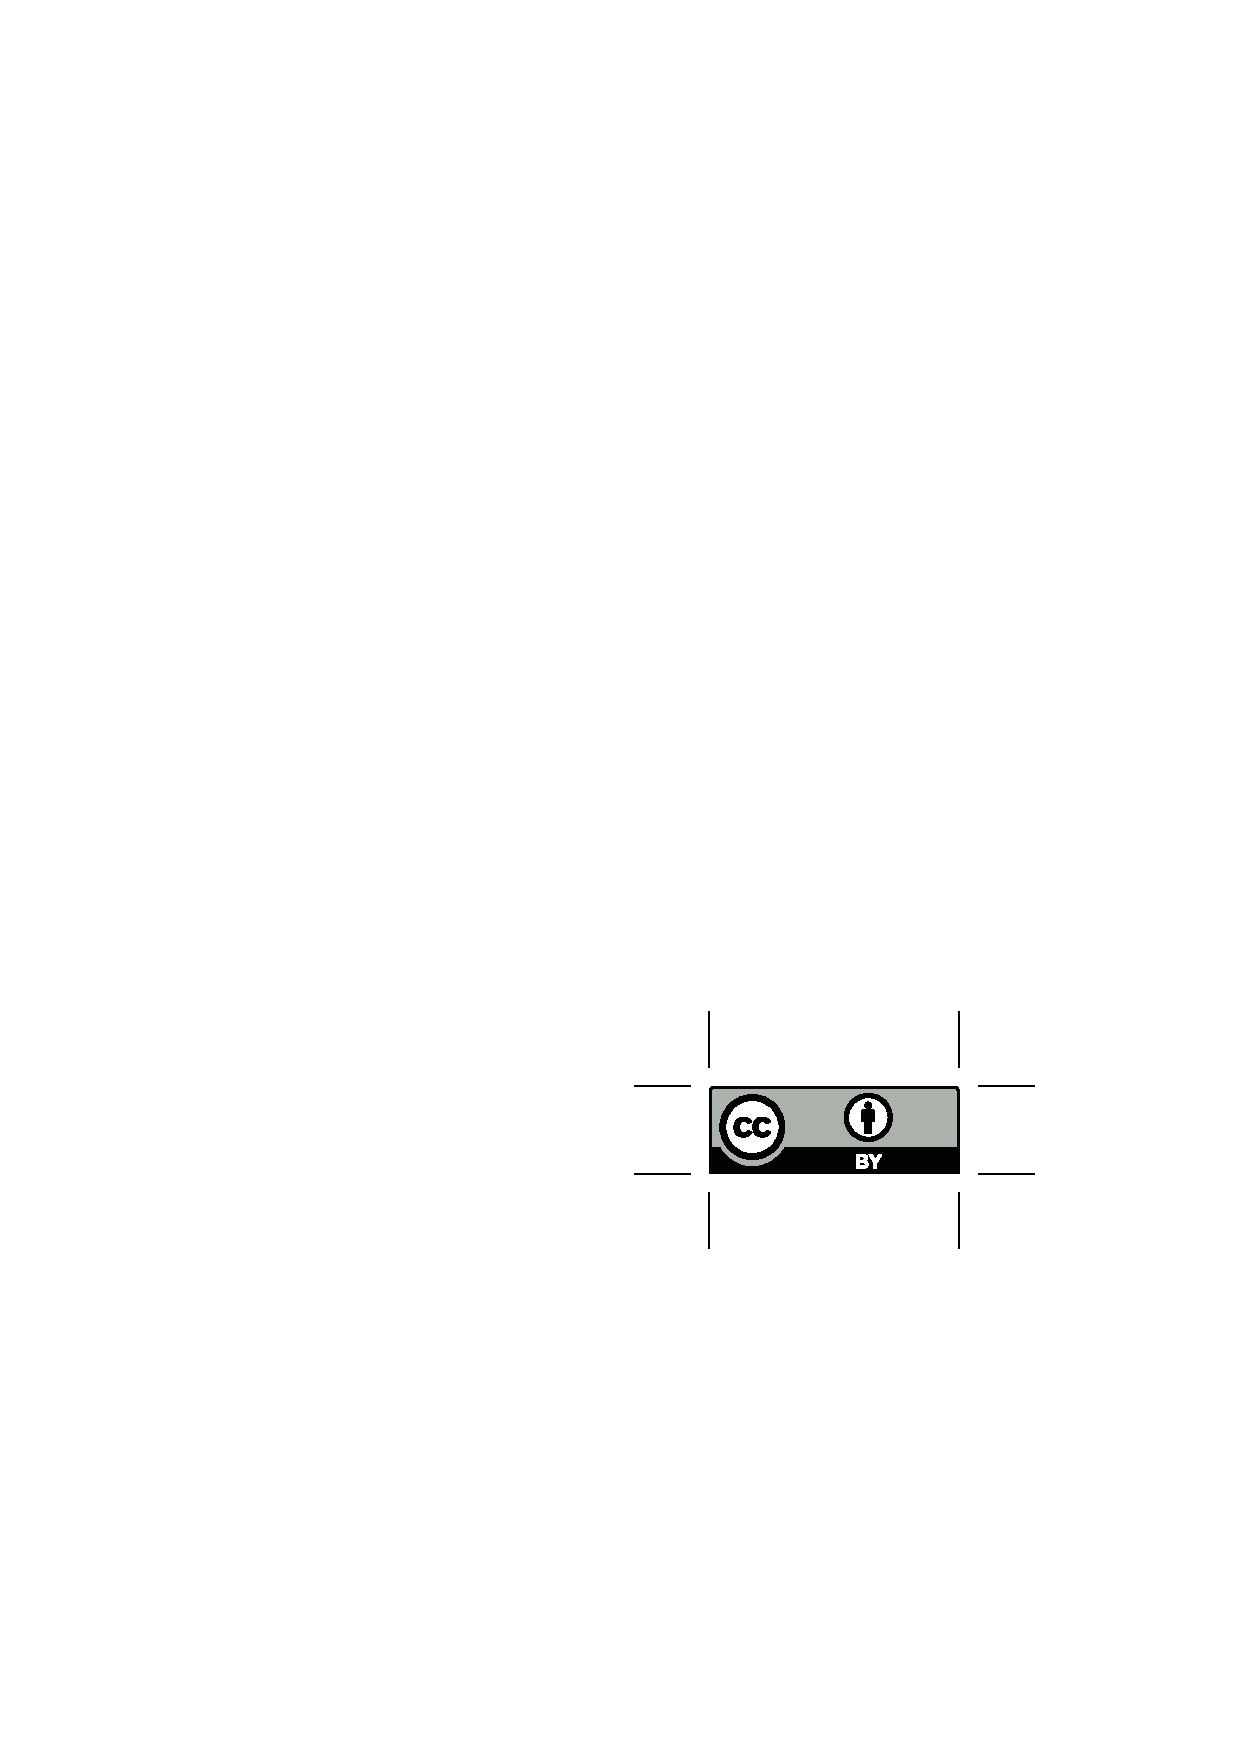
\includegraphics{images/CC-by} & 2022. \textit{Mathematics in the World Around Us} \textbf{Student Workbook} is licensed under a \href{http://creativecommons.org/licenses/by/4.0/}{Creative Commons Attribution 4.0 International License}. \tabularnewline
\end{tabular}
\par\end{center}


\newpage

% give page numbers again
\pagestyle{plain}

\pagenumbering{roman}

\tableofcontents


\newpage

\chapter*{Acknowledgements}%\markboth{Acknowledgements}{Acknowledgements}}
\addcontentsline{toc}{chapter}{Acknowledgements}

Much of the material in the intro, logic, and counting sections was remixed from work originally done at Auburn University and published under the title "Investigating Discrete Mathematics" in 2014. We thank the authors of that work for allowing us to remix, supplement, and re-license that material. It was a great aid in getting started. Work on this project was supported by a CT OER 2022 grant.

\newpage
%\cleartooddpage[\thispagestyle{plain}]

\fancypagestyle{plain}{
  \fancyhf{}% Clear header/footer
  \renewcommand{\headrulewidth}{0pt}
  \fancyfoot[L]{Southern Connecticut State University}% Right header
  \fancyfoot[C]{\thepage}% Center footer
  \fancyfoot[R]{\itshape Chapter \thechapter}
}
\pagestyle{plain}

\pagenumbering{arabic}


\setcounter{chapter}{-1}
%\part{Logic}
%<*logic.Title>
\chapter{Introductory Challenges}\label{logicProblems}
%</logic.Title>
%</logic.intro>

\setcounter{section}{-1}
\section{Mathematical Outcome}

The mathematical process is deeper than simply arriving at the correct answer. The goal of this chapter is to introduce the students and the instructor to the format of the text. The authors' hope is that the activities provided throughout the text will foster an interactive and cooperative classroom environment. This chapter is a set of logic problems which require little or no prerequisite knowledge and establish a foundation of thinking which will be used in activities throughout the text. 

You will find that the students will begin developing the basic problem solving skills throughout this chapters activities. They will encounter such questioning as; ``Is this the optimal answer?'' ``Can we show there is not a better way?''  ``Can we explain why our technique will solve the problem?'' etc. In answering these questions students are engaged in the mathematical method of developing reasoning through concrete examples.

To further this extension from the concrete to the abstract we begin asking students to change the variable of the problem to see if the previous solution technique continues to apply. In some cases a technique can be developed which will work for all possible arrangements of which it is natural to ask ``how do we know the method will work for all possibilities?'' However, the students are also exposed to solution methods which are not valid when a variable is changed. The contrast in the problems will hopefully develop the necessary curiosity which initiates the investigation process.

As a framework for the entire course, Polya's four step method for problem solving should be introduced, emphasized, and reemphasized throughout. Reference to these steps will be made from time to time within the instructor's notes, but they should be kept in the forefront of students' minds whether the prompts are there or not.

Polya's Problem Solving Method
\begin{enumerate}
\item Understand the problem (This may include reading the question several times, asking "what if" questions, tinkering with parts of the question, and so on.)
\item Devise a plan (Though this is often a completely separate step from understanding the problem, the tinkering used to understand may lead to an idea for a plan of action.)
\item Carry out the plan (When the plan can be completed, great! However, one may find they are unable to complete their plan of action due to its difficulty or faultiness. It is at this point, the method becomes iterative. The problem solver will need to revisit understand the problem or devising a plan to refine their approach.)
\item Review (Even when the plan can be carried out successfully, a review of the result is needed. Do the results answer the question asked? What evidence is there that the results are correct? Is that answer actually correct? If not, here is another place where the method becomes iterative. The problem solver will have to revisit one of the first three steps depending on the flaw identified.)
\end{enumerate}
It is important to emphasize that a natural part of problem solving is temporary failure. Noticing that there is a flaw in the solution to a problem (during the review) is a critical step in solving difficult problems. It should not be expected that anyone will devise correct, complete answers on their first try, and that this should not be considered failure. It is a temporary setback that should launch the problem solver down a new path. One only fails when one gives up trying new ideas.


\newpage

\section{Activity: Manager's Schedule}

\noindent Let's assume you are the manager for some business. This could be anything like an advertising firm, a theater production, or IT department. You have 9 projects that must be completed before your team can go on break. You predict that each project will take a day to complete and have assigned the expects needed for each project in the table below. No person can work on two projects in a single day but must be present the entire day the project is being worked on. (Maybe they are in different locations, national safety procedure require this, etc.)  Unfortunately you have to stay until all projects are completed, so you really want to create a schedule that allows yourself to go on break ASAP!

\begin{tabular} {| l | l|}
\hline
Project Number& Employees assigned\\
\hline
\hline
1 & Anna, Beth, Chris, Doug \\
\hline
2 & Eve, Chris\\
\hline
3 & Doug,Eve,Fran,Ian\\
\hline
4 & Anna, Eve, Fran\\
\hline
5 & Beth, Chris, Fran, Greg, Hugh\\
\hline
6 & Anna, Hugh, Ian\\
\hline
7 & Doug, Greg, Hugh\\
\hline
8 & Beth, Greg\\
\hline
9 & Ian \\
\hline
\end{tabular}

\begin{enumerate}

\item \label{firstschedule} Give a first attempt at making a good project schedule. Don't worry about making it on the fewest number of days yet.
\par\Instr{ We are starting to develop Polya's 4 steps in problem solving without calling them by name. We also want to establish a culture of working together and getting something on paper as soon as we start working. Even if students don't have the full or correct answer, they should right down their first attempt to get something to discuss. (I like to refer to these as a ``productive fail'' - you have a product that may have failed your overall goal, but your are progressing in the problem solving process!)}

\item Double check the schedule you made for Question \ref{firstschedule} to make sure no person is required to work on two projects in the same day. Describe or illustrate how you know your schedule has met that criteria.
\par\Instr{Here we are having the explore the features of the problem to ensure they accurately understand and can explain how a solution they created meets the problem constraints. Seemingly the easiest way for them to check is to write each project for a day and under the project list the employees assigned to that project. They may want to list all the ``inactive'' members as well just to ensure they have accounted for all 9 employees each day. 

\

We suggest at some point when most groups have finished this question to have groups share their schedules with the whole class and discuss their organization process. }

\item Create a way to organize the interactions between the project members. How will you use this information to make a project schedule with the fewest number of days?
\par\Instr{After making a schedule and seeing other groups, students should see that they cannot just simply trial and error this process. So we are now asking the students to re-examine the information from the problem and start to devise a plan by identifying all key variables, data, and or structure of the problem.}

\item \label{trivialmin}Can you easily identify a minimum number of days you will need your team to work? What is your reasoning you cannot finish any sooner?
\par\Instr{Here we are asking student to stop and identify some easy constraints. Often student get to involved in the problem and don't make simple observations or estimates for their desired solution. The simplest observation here is that every employee has been assigned to three projects, so no schedule could ever exist on fewer than three days. There is also an argument, using graph theory, that no schedule on three days can exist, but that is not an observation we expect at this point. }

\item Now create a project schedule That uses that uses the fewest number of days
\par\Instr{ This is where we are asking them to carry out their plan. Usually this is the longest period of time in the problem solving process. Notice they are already five questions into the problem before they need to really find the desired solution. This is intentional in giving the students early success and developing a sense that the problem is achievable even if it is hard.

\

There are a lot of schedules that can be made, but one on four days is the optimal solution. One tip for finding this solution is to look at project 5, which cannot be scheduled on the same day as projects 2, 3, 4, 6, or 7. Now just focus on scheduling these other five projects on two days and you will easily find a contradiction. 

\

This can be modeled with graph theory in a process called graph coloring, but at this point in the class we are simply exploring how to search for features that will help problem solve.}

\item Does your schedule get you on break as early as your answer from Question \ref{trivialmin}? If not, explain why there is no schedule that finishes faster or make a better schedule.
\par\Instr{This is the final step for polya's process, where we ask students to reflect on their solution. Assuming the student answers three days for Question \ref{trivialmin}, they will never achieve this under the constraints of the problem. In the previous explanation we have given you one reason that four days is the optimal answer, but it is not the only reason. 

Having students articulate aspects of their solution and the problem constraints is crucial in understanding the problem and being able to repeat or abstract the process. If time allows, we highly encourage groups sharing their answers to this questions for the whole class to benefit from the knowledge gained.}
\end{enumerate}

\newpage

\subsection{Exit Slip: The Manager's Process}

\noindent To help you remember what you learned for next year or possibly pass this along to the next manager

\newpage

\section{Activity: Making \$20}

\begin{center}How many different ways can you have \$20 in US bills?
\end{center}

\noindent Sometimes a simple question can have many layers, so we first must unpack and organize our thoughts before answering! We will use Polya's 4-step problem solving method to guide the process.

\begin{enumerate}

\item \textbf{Understand the problem.}
    \begin{enumerate}
        \item Can you write down three different ways to make \$20 in US bills? If yes, write them down---this is good progress toward understanding the problem! If no, a discussion with your peers is in order (What are "US bills"? What is meant by "make \$20"? etc.)
        \wbvfill
        \item What makes your three ways different?
        \wbvfill
        \item Are there other ways to make \$20? How many? (It's ok to make a wild guess at this point!)
        \wbvfill
        \item \label{billsto20} What denominations of bills are possible to use in a collection that sums to \$20?
        \par\Instr{ We begin with this simple question to make sure students are working with the same items before working toward a solution method.}
        \wbvfill
        \item Do you think you are being asked for an exact number for the total, or is an estimate good enough?
        \par\Instr{ This is a good time to steer students toward understanding that we are looking for an exact answer, not an approximation.}
    \end{enumerate}

\wbvfill
\item \textbf{Devise a plan.}
    \begin{enumerate}
        \item \label{20witha1} Provide an example of a collection of bills that sums to \$20 that contains exactly one \$1 bill?
        \par\Instr{ There are many possibilities for such a collection of bills but each would need to contain at least two \$2 bills. This is meant to spark the students to think about the need for the \$2 bill if they missed it above and get them thinking about how they are going to organize their collections. If they have not thought about the \$2 bill, they would say it is impossible with a reasoning about how all other denominations being a multiple of $5$ but $20-1 = 19$ is not a multiple of $5$. Maybe they will list several solutions. If so, you might ask if they have them all and how they know.}
        \wbvfill
        \item \label{20witha1andno5} Is it possible to have a collection of bills that sums to \$20 that contains exactly one \$1 bill and no \$5 bills? If so provided an example or explain why none exists?
        \par\Instr{ This is impossible because using exactly one \$1 bill leaves us with \$19 remaining dollars but the only remaining bills (\$2, \$10, \$20) have even denominations so will never total $19$. A deeper look into this concept could produce the idea that any collection totaling \$20 must contain an even number of odd denomination bills. This question can spawn some deep thought into the ideas of parity and generating sets, but that is deeper than we expect students to take this topic. We will ultimately not use this approach, but it is a good example of the brainstorming process and the fact that some ideas will ultimately not be pursued.}
        \wbvfill
        \wbnewpage
        \item \label{making5} \textbf{One of the best ways to start problem solving is to solve a simpler similar problem.} One way to do that is to work on a lower total. List all the ways that U.S. bills can make a total of $5$ dollars. HINT: There are more than two ways.
        \par\Instr{ There are four ways. Besides illustrating the "solve a simpler problem first" technique, the purpose of this question is to start the students thinking of how they will list out a collection of bills and to help the student realize they have three denominations of bills to work with---many times students will forget about the \$2 bill!}
        \wbvfill
        \item \label{making10} Let's continue our exploration of simpler problems. Write down all the collections of bills that make \$10.
        \par\Instr{ This is meant to make sure the students are all on the right track before answering the larger question. It will also be useful in answering a later question. We suggest you stop the class at some point and have a group present their solution and \textbf{have a class discussion on tree diagrams}. The 11 solutions are written out in bill denominations below.\\
            (1) 10\\
            (2) 5-5\\
            (3) 5-2-2-1\\
            (4) 5-2-1-1-1\\
            (5) 5-1-1-1-1-1\\
            (6) 2-2-2-2-2\\
            (7) 2-2-2-2-1-1\\
            (8) 2-2-2-1-1-1-1\\
            (9) 2-2-1-1-1-1-1-1\\
            (10) 2-1-1-1-1-1-1-1-1\\
            (11) 1-1-1-1-1-1-1-1-1-1
        }
        \wbvfill
        \wbvfill
        \item Did you use the result from \ref{making5} in solving \ref{making10}? If no, what is one way you could have? HINT: See if you can find a connection between your answer to part \ref{making5} and your answer to part \ref{making10}.
        \par\Instr{ 4 of the collections that make \$10 start with a \$5 bill. That there are 4 is no accident. Starting with a \$5 bill means the remaining bills must sum to \$5, and there are 4 ways to do this as seen in the solution of part \ref{making5}. In other words, the solution to part \ref{making10} could have been written as\\
            (1) \$10\\
            (2,3,4,5) \$5 (with 4 ways to make the remaining \$5 as seen in \ref{making5})\\
            (6) 2-2-2-2-2\\
            (7) 2-2-2-2-1-1\\
            (8) 2-2-2-1-1-1-1\\
            (9) 2-2-1-1-1-1-1-1\\
            (10) 2-1-1-1-1-1-1-1-1\\
            (11) 1-1-1-1-1-1-1-1-1-1
        }
        \wbvfill
        \wbnewpage
        \item \label{20highest1}Another way to solve a similar simpler problem is to make the total \$20 but restrict the types of bills that may be used. List all the ways to make \$20 where the highest denomination is a \$1 bill (meaning you must use at least one \$1 bill and no higher denominations).
        \par\Instr{ This should be an obvious answer that we must use twenty \$1 bills.}
        \wbvfill
        \item \label{20highest2}List all the ways to make \$20 where the highest denomination is a \$2 bill (meaning you must use at least one \$2 bill and no higher denominations).
        \par\Instr{ There are ten since you may use from 1 to 10 two-dollar bills (completed to \$20 using ones).}
        \wbvfill
        \wbvfill
        \item How do you know there are no repeats in your answers to questions \ref{20highest1} and \ref{20highest2}?
        \par\Instr{ Students may be tempted to say something like "There is only one way in \ref{20highest1} and I can see it is not in the list for \ref{20highest2}. That's not bad, but the real point is that the highest bill in the collections for \ref{20highest2} is 2, and the highest bill in the collections for \ref{20highest1} is 1. Assuming these questions are answered correctly, you know there will be no repeats before you even start. Each set has a different highest denomination. No single collection can have two separate highest denominations so no single collection can be in multiple lists.}
        \par\Instr{ It may seem strange to organize our questions this way, but we are trying to make the lists a bit smaller and also lead students into breaking up their solutions into disjoint sets. There are always many ways to organize a solution set, but it is most natural to think of organizing our bills in descending order. Also, this way is conducive to utilizing a tree diagram to list all of our solutions.} 
    \end{enumerate}
    \wbvfill
    At this point we have explored two ways to create simpler similar problems (restrict the total dollar amount and restrict the types of bills we can use), and we've seen that one simpler solution may be used to solve another (using the \$5 totals to help make the list of \$10 totals). Using one or both of these ideas, devise a plan for finding all collections of US bills that make \$20. Summarize your plan here. DO NOT carry out the plan here. Just describe a plan that you think will work.
    \wbvfill
    \wbvfill
    \wbnewpage
    \item \textbf{Carry out the plan.} Try to do what you just described to find out how many different ways there are to make \$20 using US bills. If you are struggling to make your plan work or you have determined that it just won't work, go back and revise your plan!
    \par\Instr{ One way to proceed is to make a tree diagram as below (or a table with the same information), using smaller problems already solved so not every branch needs to be shown.
    \begin{center}
        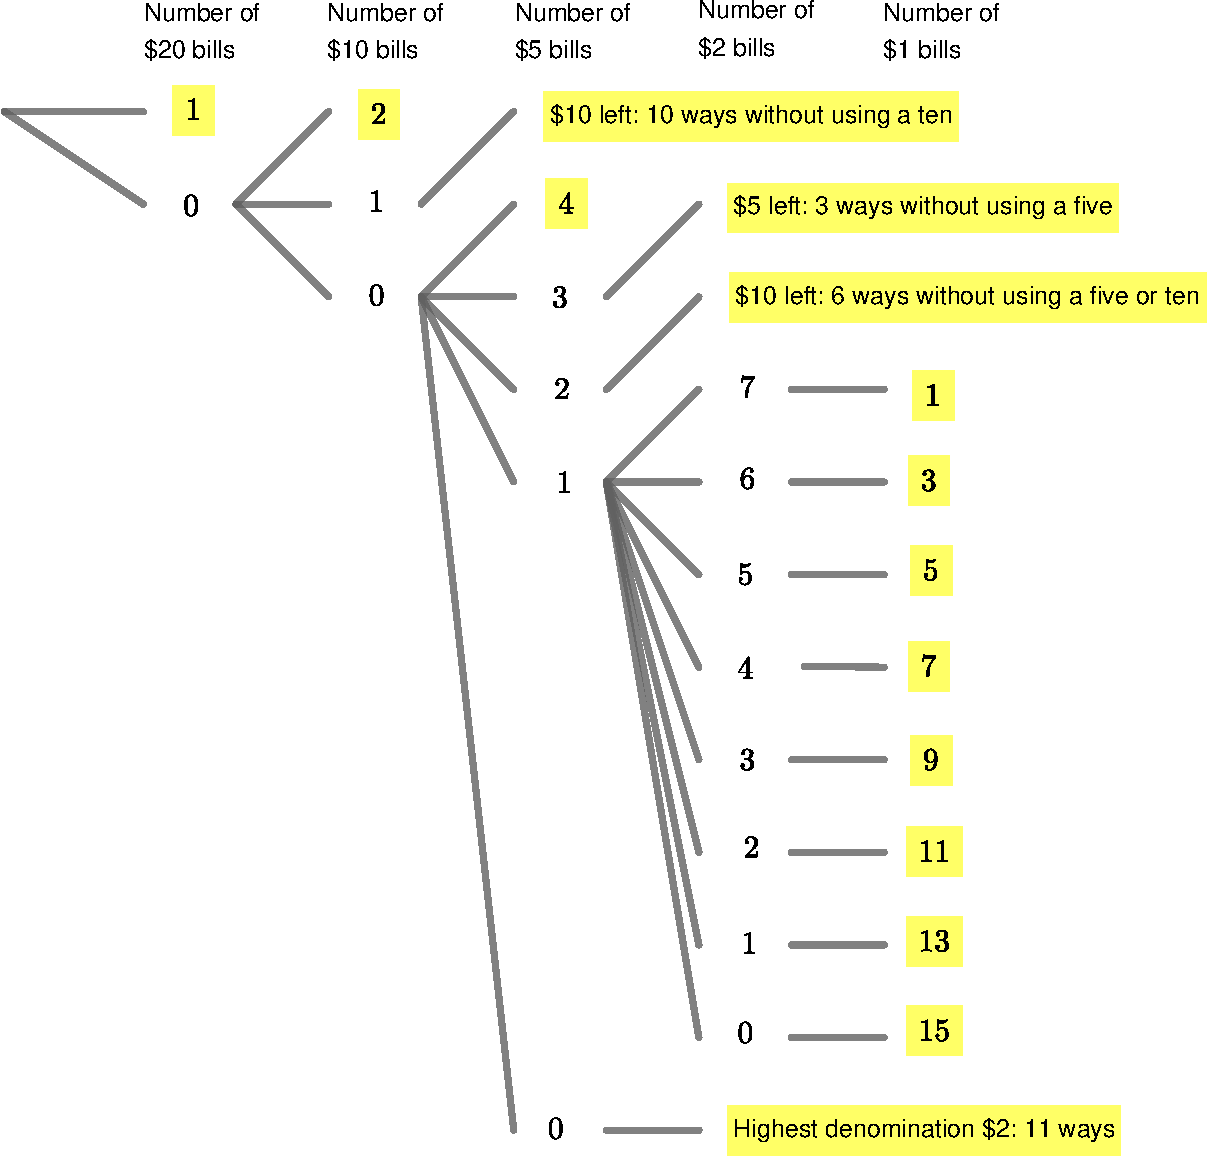
\includegraphics[width=5.5in]{images/Make20dollarsTree2.pdf}
    \end{center}
    }
    \par\Instr{ Another way to solve this problem is along the following lines.
    \begin{enumerate}
        \item \label{20withno10s} Determine the number of collections of bills that sum to \$20 and contain no \$20 bills or \$10 bills.
        \par
        This question is asking about the branches that do not begin with a \$10 or \$20 bill. So the first bill in each collection is below 10 and so the tree diagram will begin with three branches and proceed accordingly.
        \par The full tree diagram should look something like what is shown in Figure\ref{Making20Tree} producing $29$ total collections with no \$10 or \$20 bills. Notice there are key aspects of this tree that are worth exploring. Two key aspects mentioned above are:
        \begin{enumerate}
            \item Each branch has a bill denomination less than or equal to the branch it is stemming from.
            \item the branches that first use a \$5 bill must have a \$1 or another\$5 bill because of the necessity of an even number of odd denomination bills.
        \end{enumerate}
        \begin{figure}[htb]
            \begin{center}
                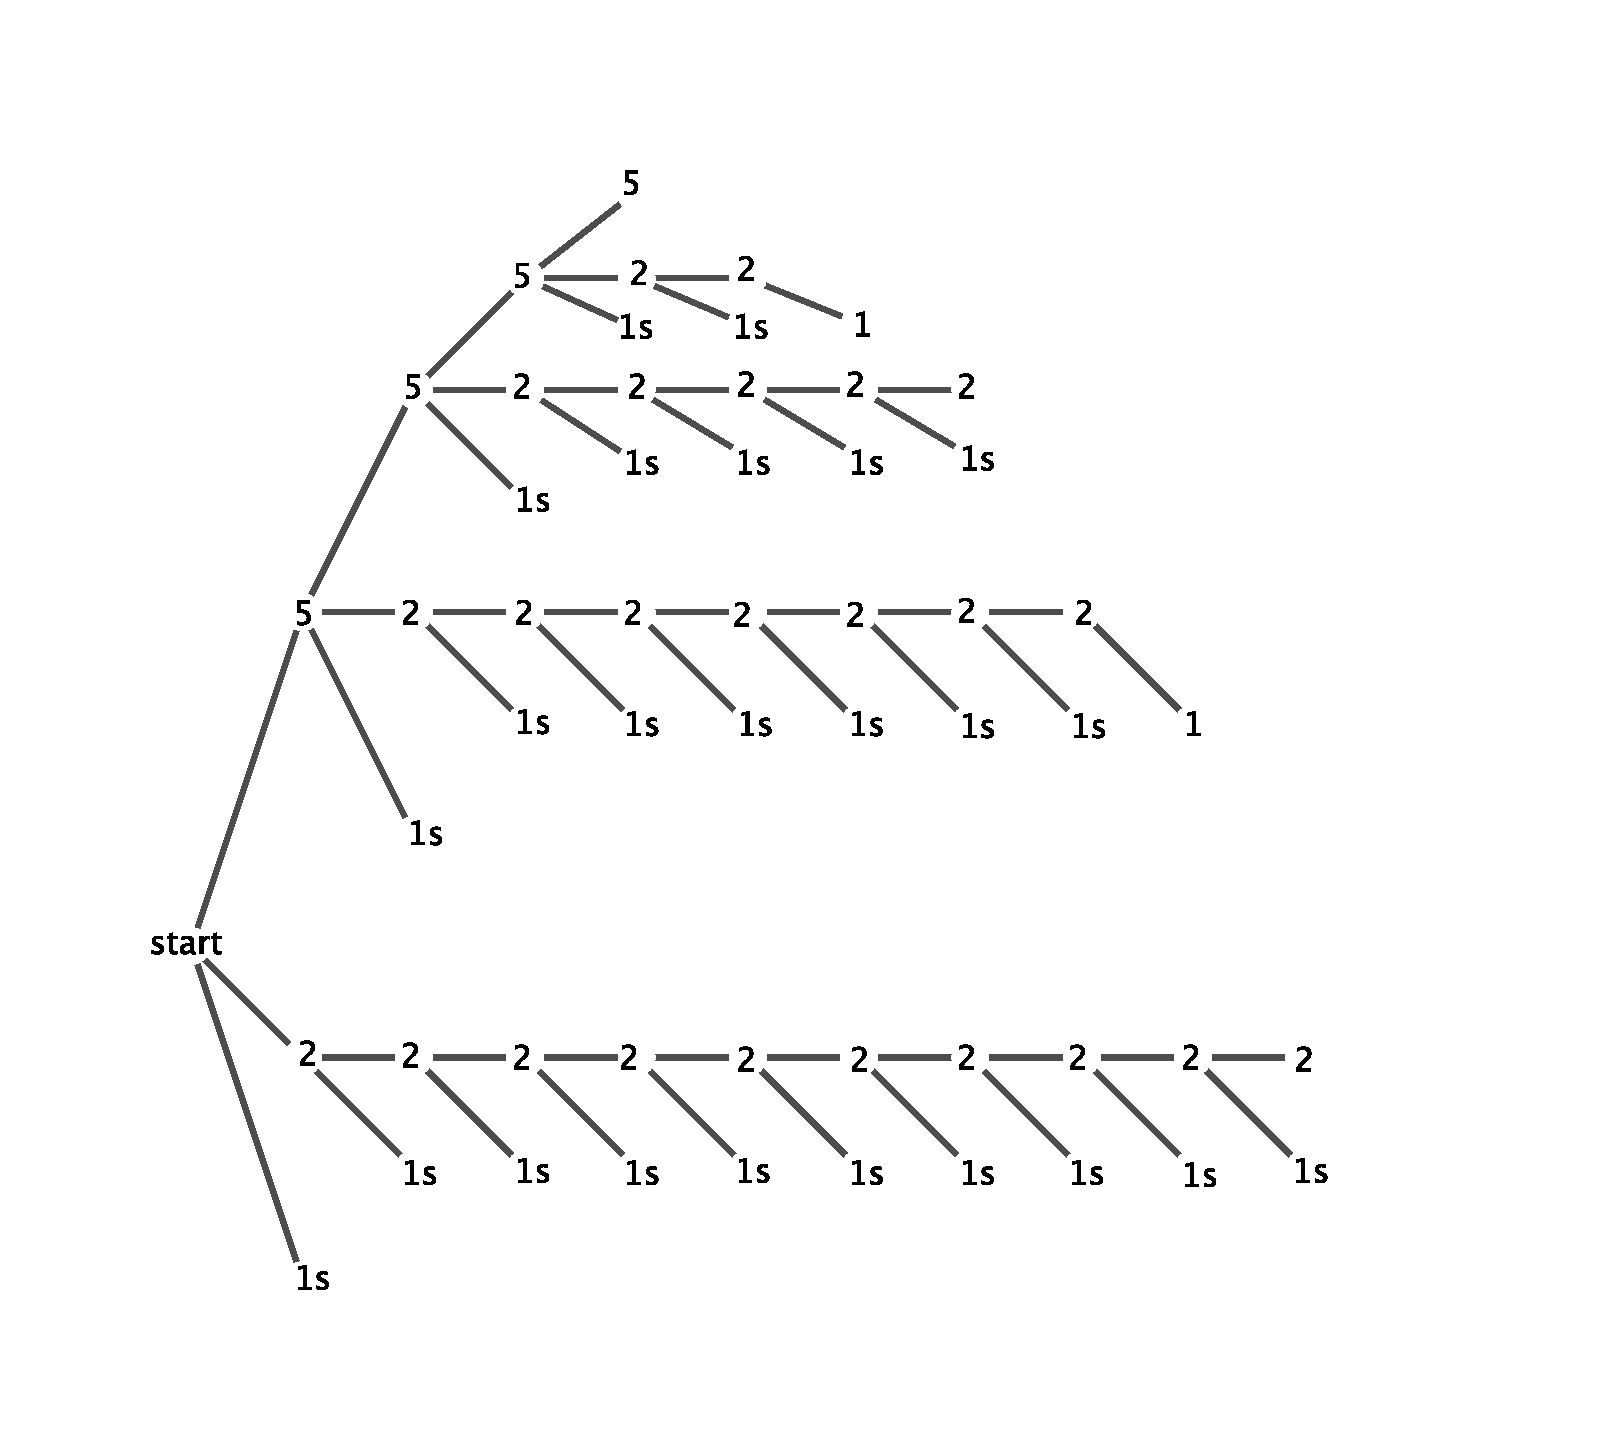
\includegraphics[width=5in]{images/Making20Tree.pdf}
            \end{center}
            \caption{ The entire solution tree for \$20 with no \$10 or \$20 bills}\label{Making20Tree}
        \end{figure}
        \item \label{20witha10} Determine the number of collections of bills that sum to \$20 and contain a \$10 bill.
        \par For the tree diagram organization method, this question is asking about the branch that begins with a \$10 bill. 
        \par We could create a tree diagram for this, but the existence of a \$10 bill leave us with needing a collection of ten more dollars. This was already solved in \ref{making10}. Therefore we know there are 11 collections of bills making up $20$ dollars that include a \$10 bill.
        \par Now the answers to the previous two questions can be added to the solution of using a single \$20 bill to solve the ultimate question. We get $1 + 29 + 11 = 41$ different ways to get a collection of bills that make \$20.
        \end{enumerate}
    }
    \wbvfill
    How many ways did you come up with?
    \par\Instr{ There are 41 ways. Counting the highlighted branches in the tree diagram above, there are 11 individual collections plus $10+3+6+11=30$ more for a total of 41.}
    \wbnewpage
    \item \textbf{Review the solution.}
    \begin{enumerate}
        \item How do you know you have not counted any collection more than once? In other words, how do you know each of your collections is different?
        \par\Instr{ As before, hopefully this will be more insightful that just saying "I checked my lists and didn't see any duplicates." It must rely on the fact that the smaller problems solved are disjoint.}
        \wbvfill
        \item How do you know you have all collections that make \$20? How do you know you have not missed any?
        \par\Instr{ This may be a tougher question to answer depending on the plan devised and carried out. But is students follow the suggestion in the exercises it may be something like "We listed all the ways to make \$20 where the highest denomination is \$1, where the highest denomination is \$2, and so on with highest \$5, \$10, and \$20. There are no other choices because using higher denominations than \$20 will give a total greater than \$20."}
        \wbvfill
    \end{enumerate}
    If you can't answer these questions or you have doubts that you have the correct answer you may need to revise your plan or how you carried it out.
\end{enumerate}

\newpage
\subsection{Exit Slip}
\begin{enumerate}
    \item How many different ways can you have \$15 in US bills? Provide a tree diagram, an organized list, or written justification for your answer.
    \par\Instr{ There are 22.
        \begin{center}
            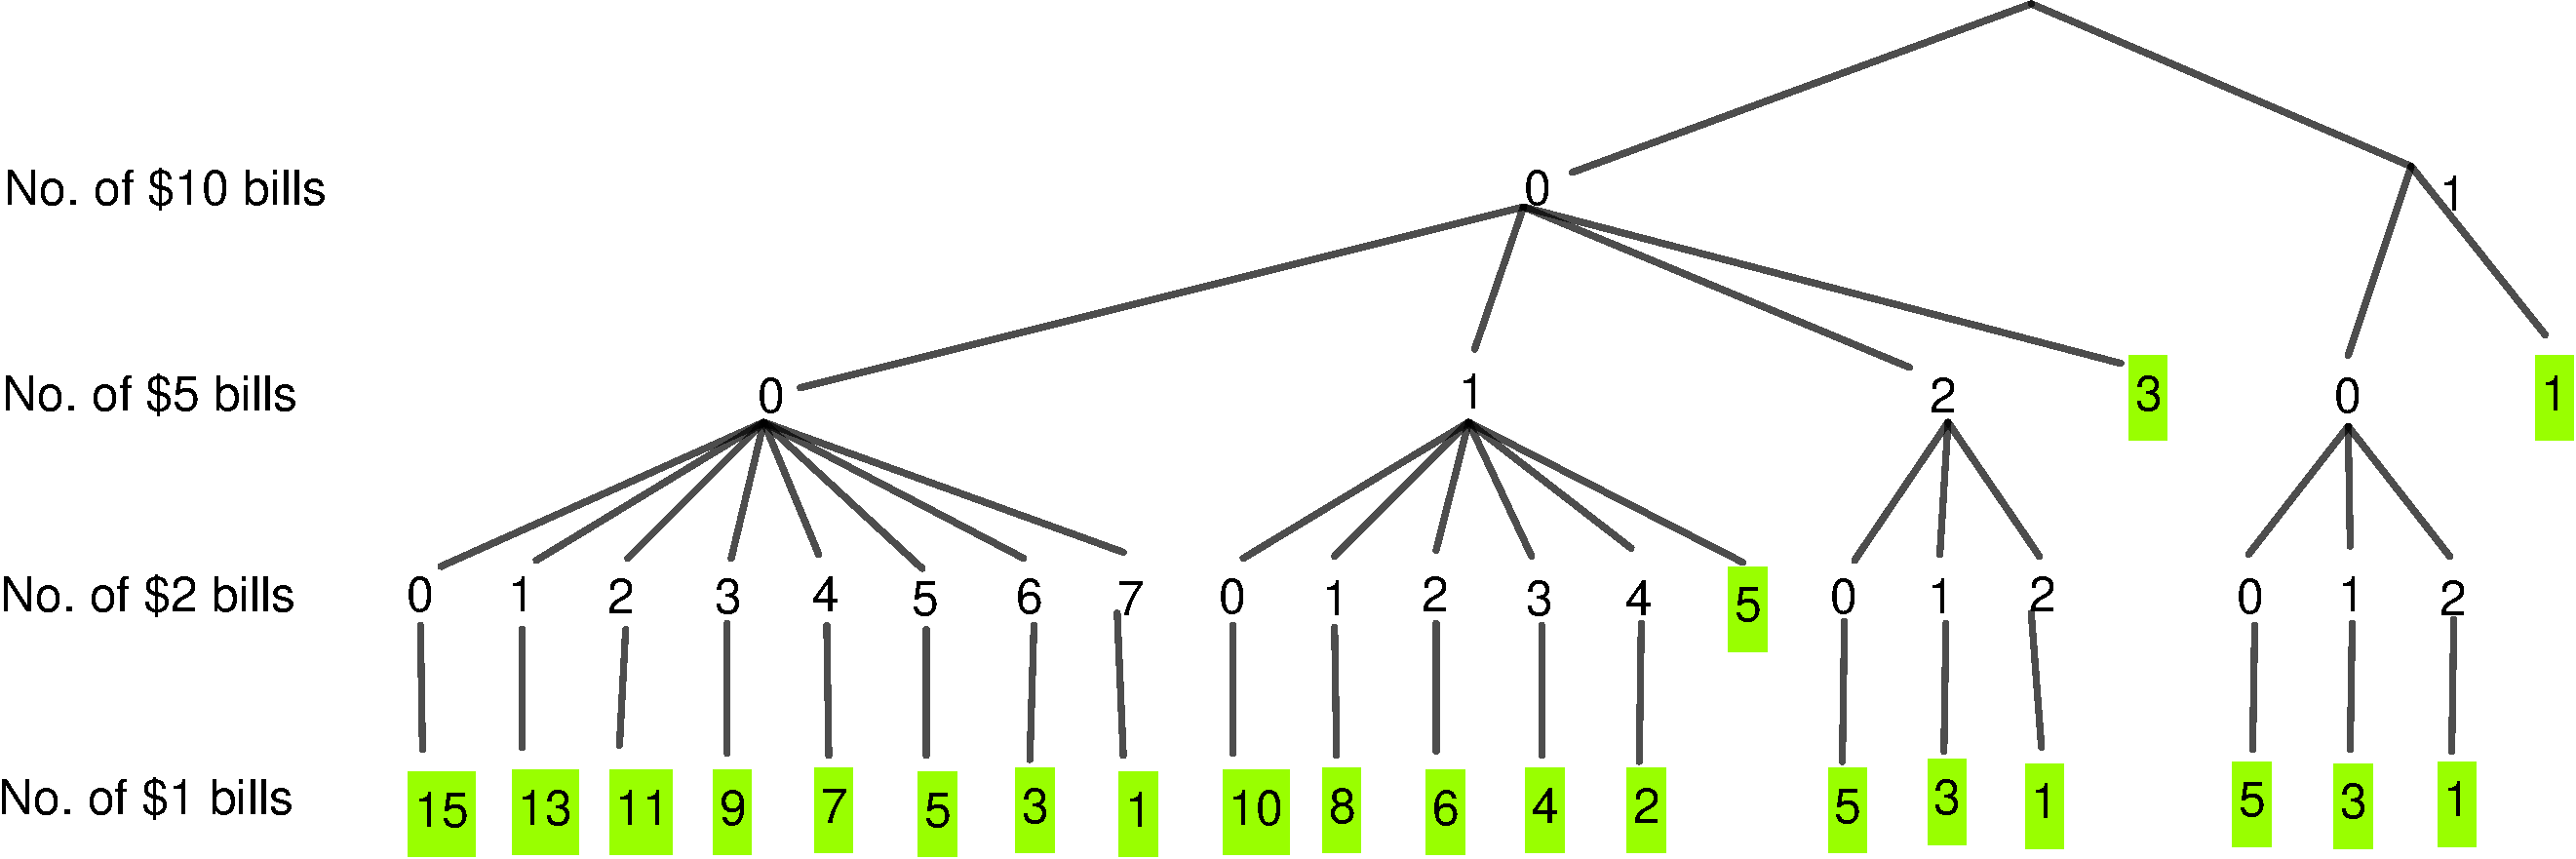
\includegraphics[scale=0.3]{images/Tree-FifteenDollars.pdf}
        \end{center}
    }
\end{enumerate}
For the remaining two questions, your solution must include (i) the tree diagram, (ii) the answer, and (iii) a few sentences describing why you believe your tree diagram gives the correct answer (shows all the answers and no repeats).
\begin{enumerate}
    \setcounter{enumi}{1}
    \item Solve \textbf{ONE} of the following problems using a tree diagram. 
    \begin{enumerate}
        \item At Panera Bread, you are presented with the following lunch choices: a starter of soup or salad; 3 different sandwiches; and a side of bread, chips, or an apple. How many different lunches consisting of one starter, one sandwich, and one side can be made?
        \par\Instr{ There are 18. This one can be calculated using the multiplication principle: $2\times 3\times 3=18$.
            \begin{center}
                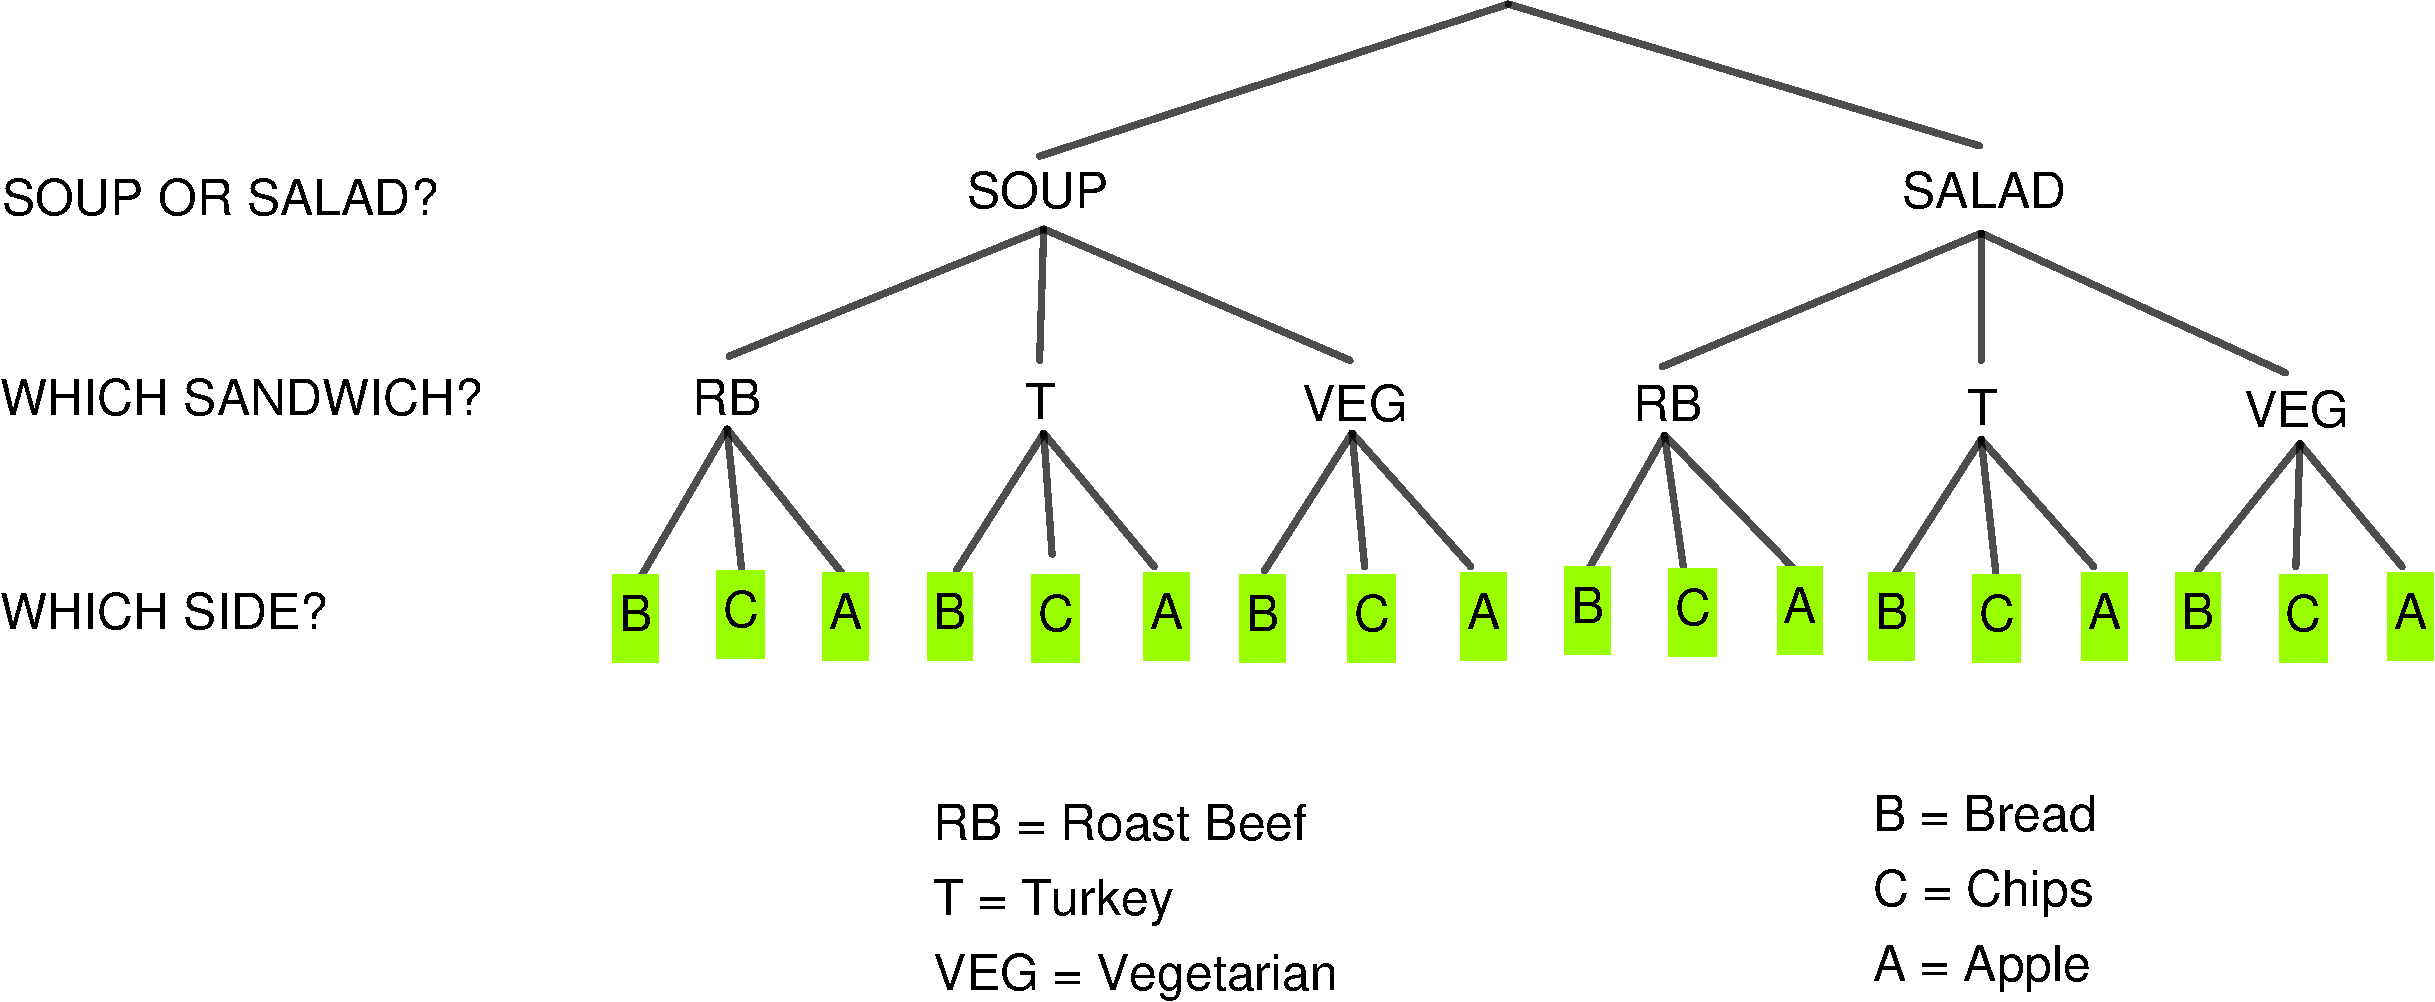
\includegraphics[scale=0.3]{images/Tree-Panera.pdf}
            \end{center}
        }
        \item At Domino's Pizza, the following unusual vegetable toppings are available: jalapeno peppers, roasted red peppers, spinach, and basil. How many different unusual veggie pizzas can you make using these toppings?
        \par\Instr{ There are 15. The N-N-N-N branch has none of the toppings so does not qualify as an unusual pizza. It is just plain cheese!
            \begin{center}
                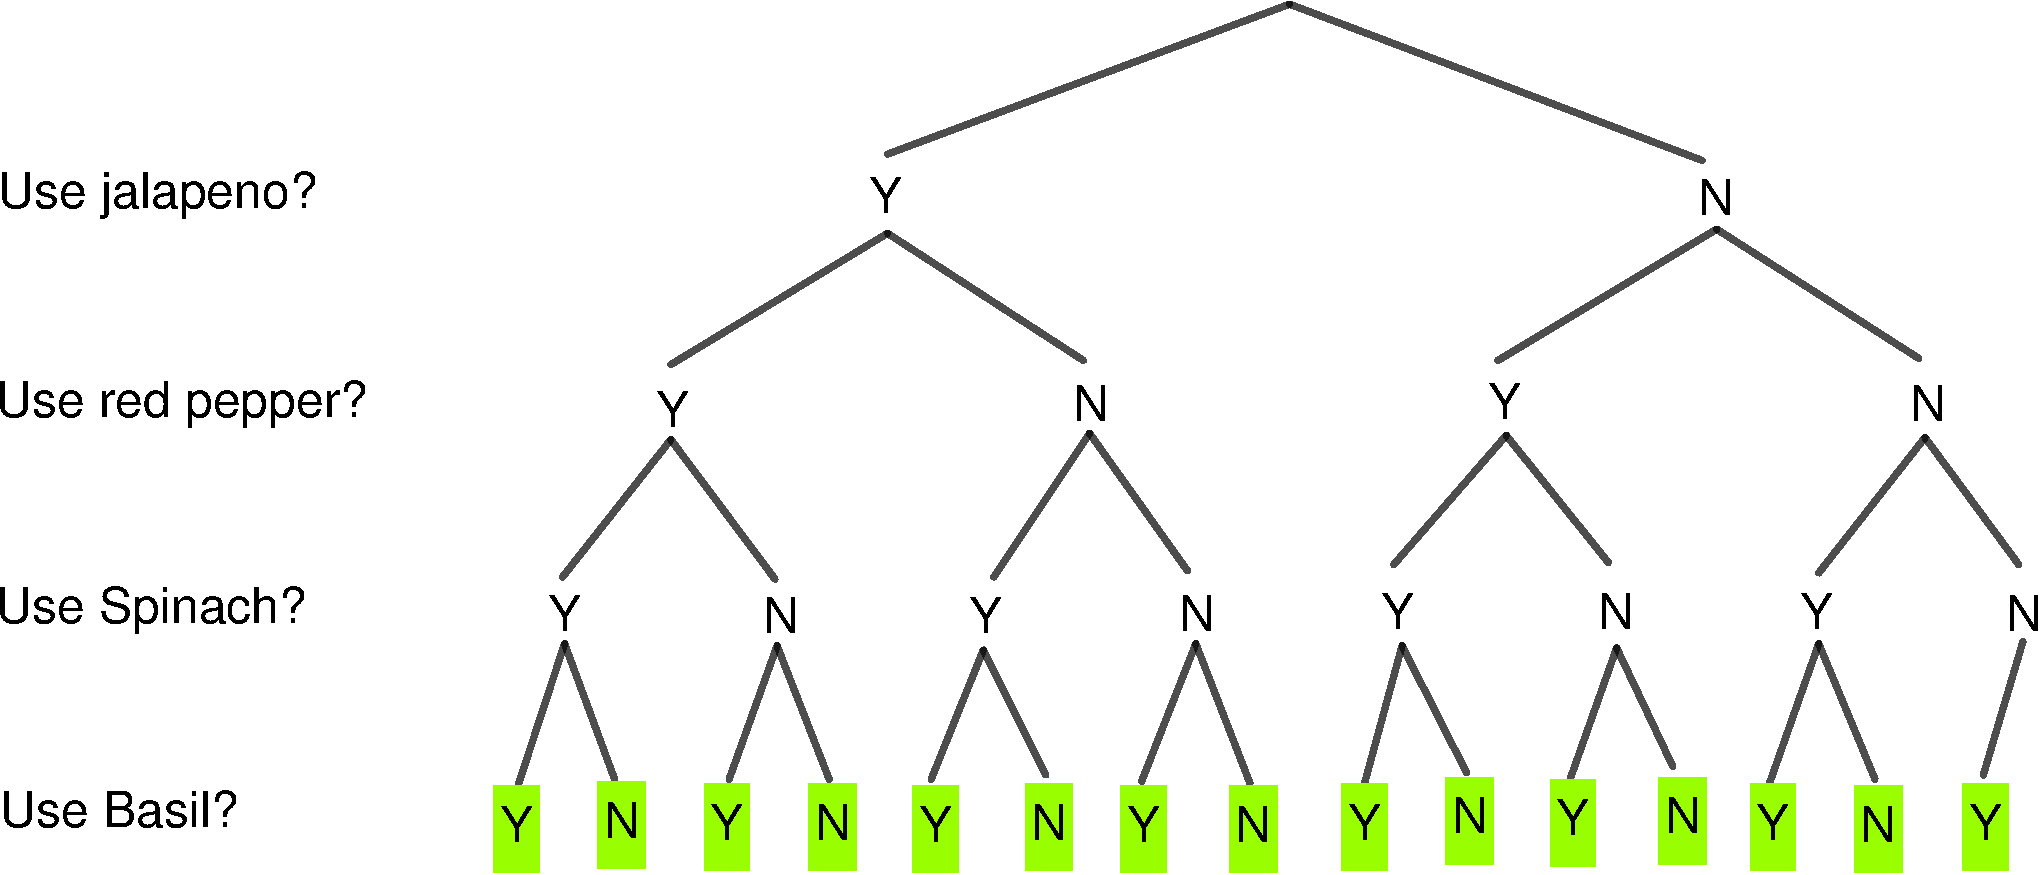
\includegraphics[scale=0.3]{images/Tree-Pizza.pdf}
            \end{center}
        }
    \end{enumerate}
    \item Solve \textbf{ONE} of the following problems using a tree diagram.
    \begin{enumerate}
        \item The division championship in major league baseball goes to the winner of a best-of-5 series. The first team to win 3 games wins the division, so the series will never go more than 5 games. For example, if the teams are Boston and Tampa Bay (as they were in the 2021 American League Division Series), one way it could have unfolded was B-T-B-T-T, meaning Boston won the first, Tampa Bay won second, Boston won the third, and then Tampa Bay won the fourth and fifth games. It also could have unfolded T-B-B-B (and this is what actually happened in 2021). How many different ways could the division series have unfolded (including the two already mentioned)?
        \par\Instr{ There are 20.
            \begin{center}
                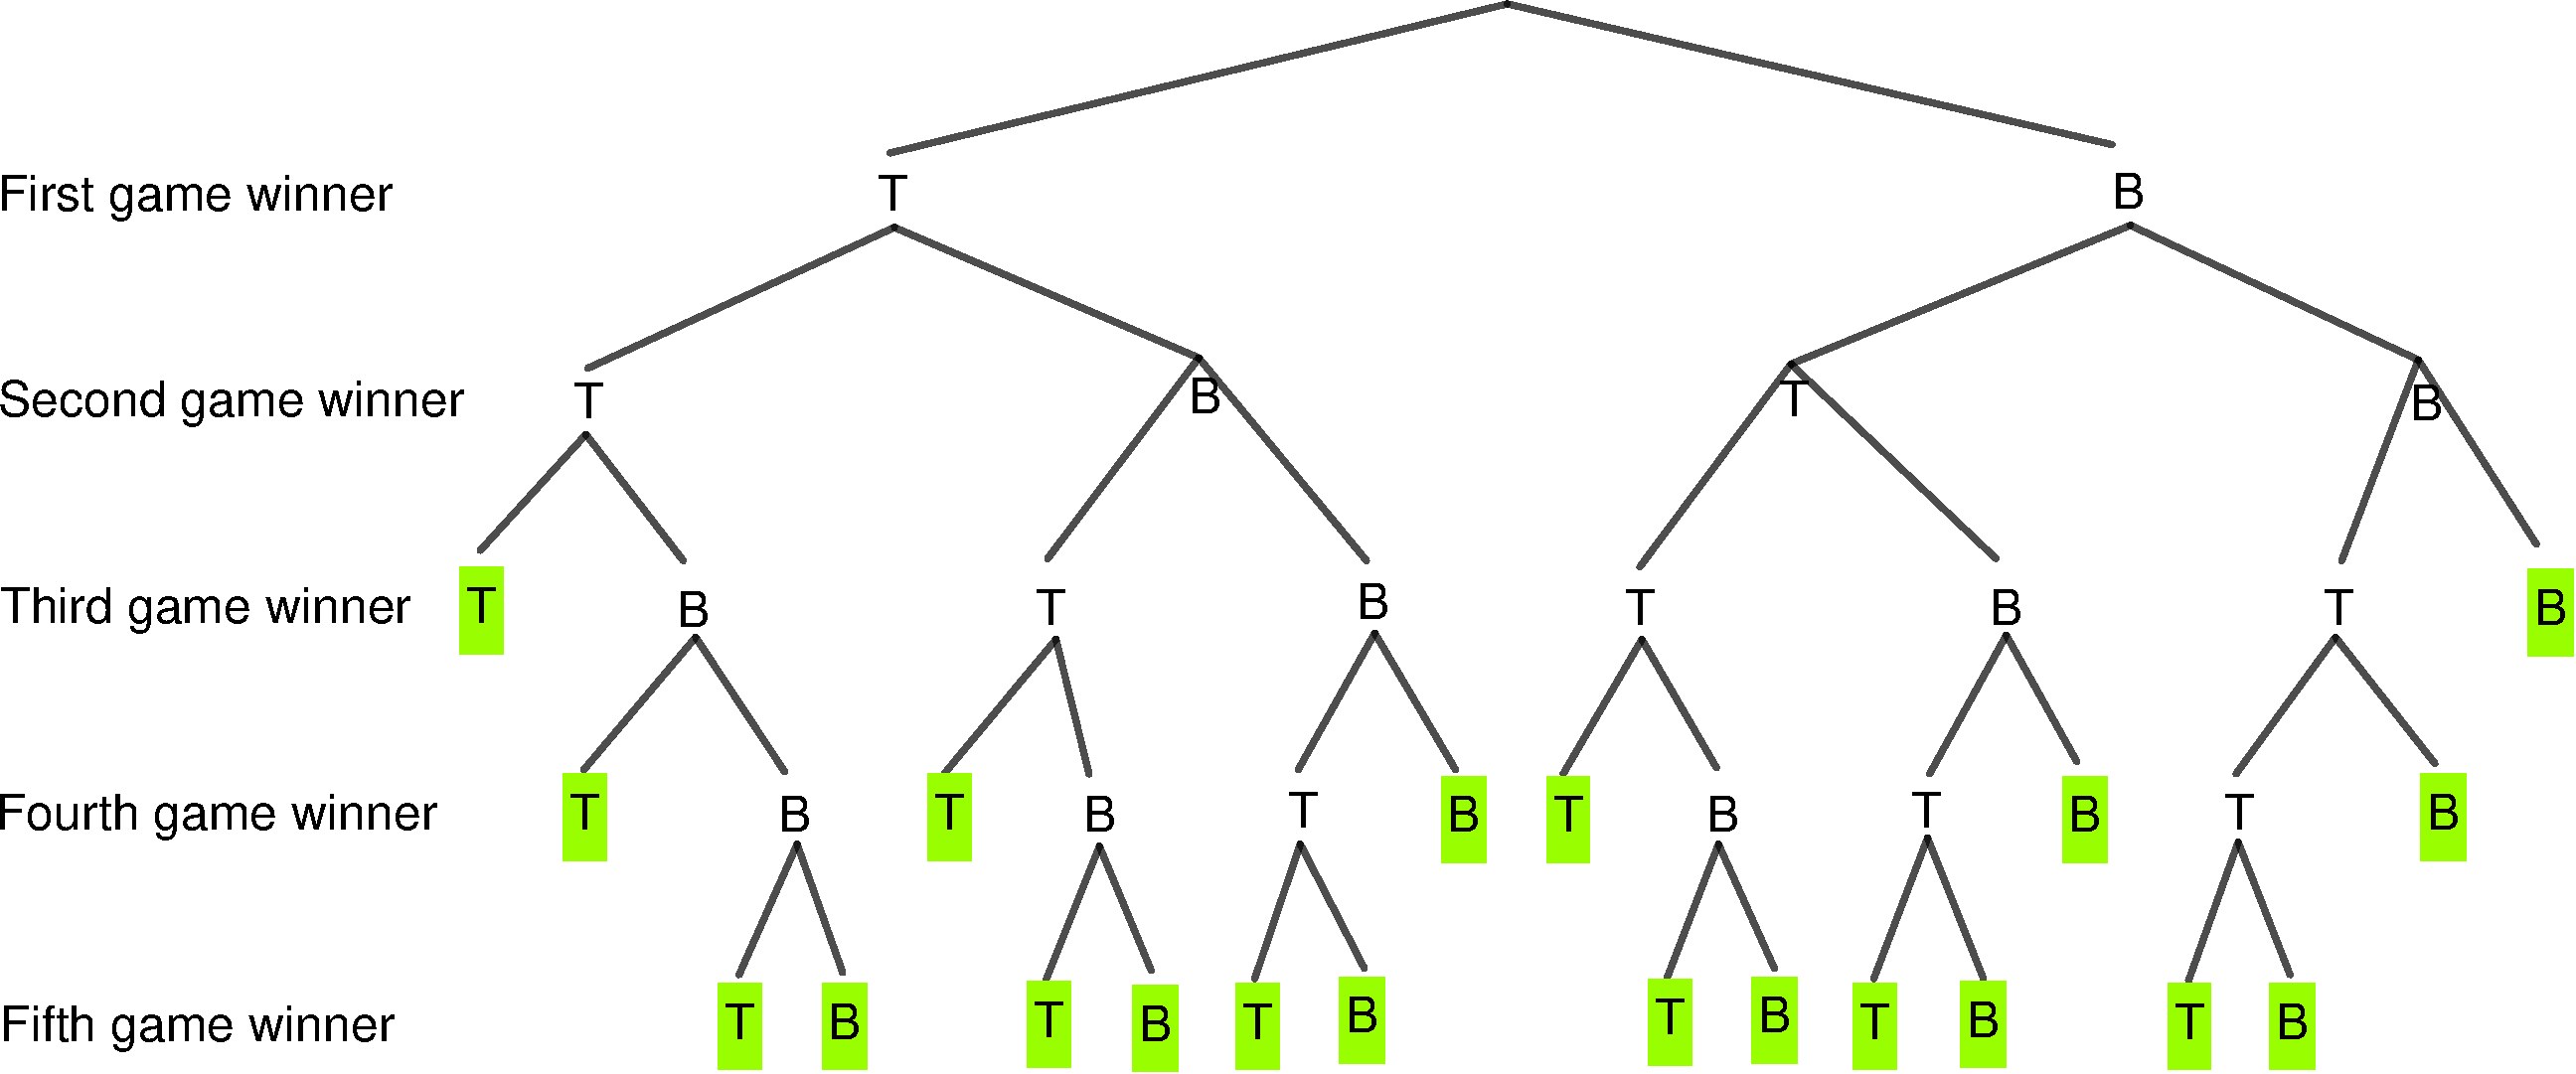
\includegraphics[scale=0.3]{images/Tree-DivisionSeries.pdf}
            \end{center}
        }
        \item The curator at a natural history museum is designing a penguin display. He would like to put penguins of 4 different species in the display---Emperor, Northern Rockhopper, Macaroni, and African---arranged one next to the other in a row. However, he wants to be sure the Emperor Penguin is not next to the Macaroni Penguin. How many ways can he arrange the penguins in the display?
        \par\Instr{ There are 12.
            \begin{center}
                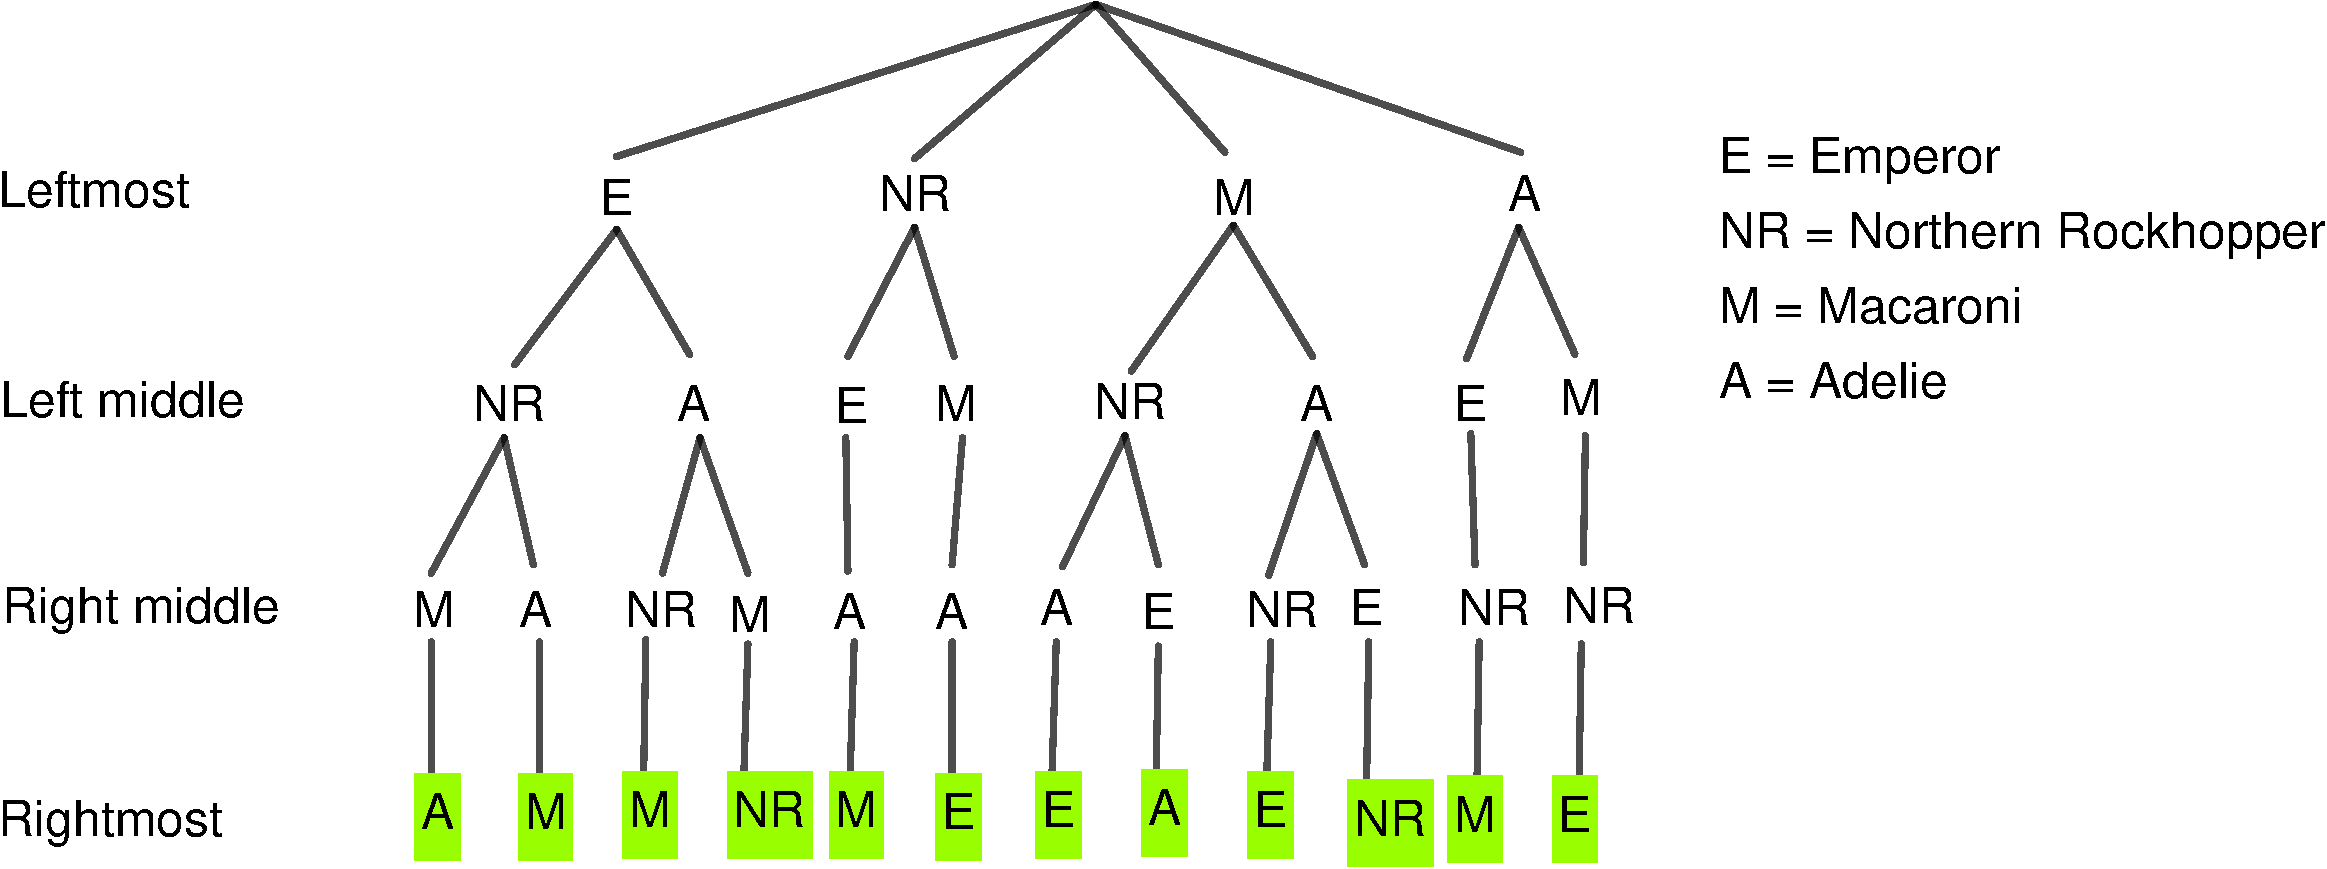
\includegraphics[scale=0.3]{images/Tree-Penguins.pdf}
            \end{center}
        }
    \end{enumerate}
\end{enumerate}

%%%%%%%%%%%%%%%
% New Section %
%%%%%%%%%%%%%%%
\newpage
\section{Activity: Crossing the Bridge}

\Instr{  
Goals for this activity:
\begin{packedItem}
\item develop problem solving and sense making; 
\item introduction to tree diagrams; and
\item using natural logical arguments (such as quantifiable bounding, negations, case arguments, etc.).
\end{packedItem}

Especially at the beginning of the course, it is important to make sure that the students understand the constraints of the problem; so, as a class, take some time to read the question and discuss the requirements. Some students may prefer to use manipulatives to solve this problem. Different sized blocks could be used to represent each person, and you also may want a small block for the flashlight. 

You may want to have the students act out their solutions. If so, it helps if each person holds a sign indicating their weight so that the rest of the class can check to see that each movement is ``legal.'' You could even ask one of the groups secretly to make a mistake on purpose to see if the other students were paying attention. }

%<*logicProblems:crossBridge:intro2>
\indent {\bf A}lfred, {\bf B}ruce, {\bf C}athy, and {\bf D}oug were coming back to their village in the middle of the night. The tiny bridge to the town is too small for more than $2$ people to cross it at the same time, and it is only safe to cross if someone is holding a flashlight. Since they only brought one flashlight, someone will have to return with the flashlight before two more people can cross. Doug can walk across the bridge in $10$ minutes, Cathy takes $5$ minutes to cross, Bruce can skip across in $2$ minutes, and Alfred can cross the bridge in $1$ minute. Unfortunately, when you walk across the bridge with someone else, you can only cross the bridge at the speed of the slower person. What is the least amount of time needed to get everyone across the bridge?
\begin{enumerate}
\item \textbf{Understand the Problem:} Act out the situation. Members of your group will play the roles of Alfred, Bruce, Cathy, and Doug. If you are a group of 3, you will only be able to play Alfred, Bruce, and Cathy. Use a prop for the flashlight and define a physical space in the classroom that will stand in as the bridge. Play act until you have successfully gotten everyone across the bridge. Are the rules clear?
\item \textbf{Devise a plan:} Solve a simpler problem first. Imagine Doug is ill and therefore not with the group. What is the quickest way for Alfred, Bruce, and Cathy to get across the bridge?
\par\Instr{ 8 minutes. The most efficient way for the three to cross is to have Alfred escort Bruce and Cathy one at a time across the bridge. The two trips take 2 minutes and 5 minutes (with Alfred being held back to the slower speed each time. After delivering one of them Alfred has to make the trip back to retrieve the other. This trip takes 1 minute as Alfred is on his own. The total time for the three trips is 8 minutes.}
\wbvfill
\item How do you know this is the quickest way? Construct a tree diagram of all the ways they can cross the bridge without any obvious waste of time (repeating a position---going from one position to another and then back to the position you were before---is an obvious waste of time).
\par\Instr{ Two ways of the six total are optimal.
    \begin{center}
    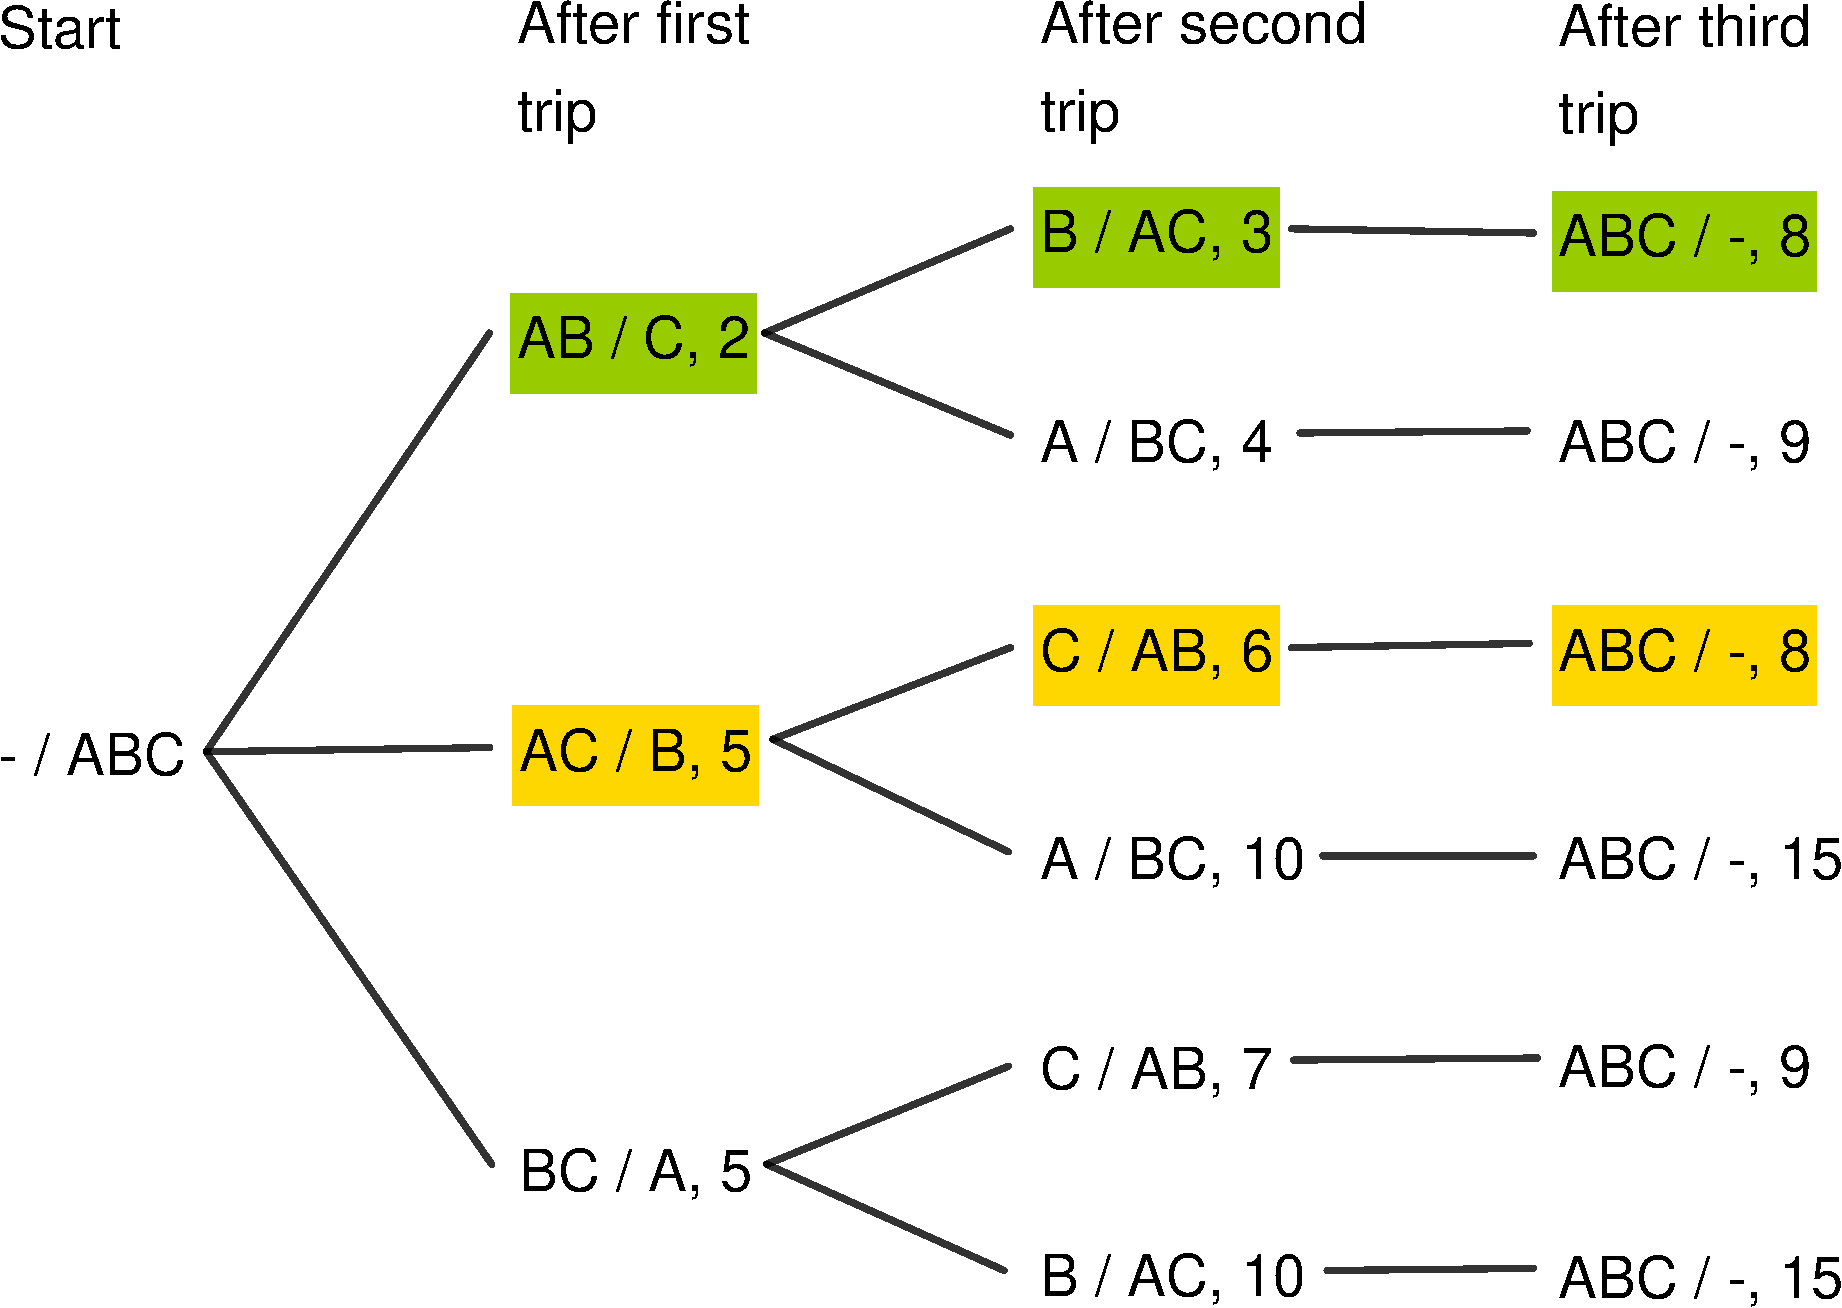
\includegraphics[width=4.5in]{images/Bridge-ABC.pdf}
    \end{center}
}
\wbvfill\wbvfill
\item For each way of crossing the bridge, calculate the total time. What is the least? How can it be done? Are there more ways than one?
\wbvfill\wbnewpage
\item\label{19min} \textbf{Carry out the plan.} Now return to the original problem and use the same process as you used for the simpler problem. What is the least amount of time needed to get everyone across the bridge? How can it be done?
%</logicProblems:crossBridge:intro2>

\Instr{ The most common answer for this problem is to make Alfred cross with each person and come back with the torch each time. In this way it will take $10$ minutes for Doug to cross with Alfred and $1$ minute for Alfred to return with the torch. Then it will take $5$ minutes for Cathy to get across the bridge with Alfred and $1$ minute for Alfred to return again. Finally, it takes $2$ minutes for Bruce to get across with Alfred. By adding all the times together it will take a total of $10+1+5+1+2=19$ minutes.

There is a quicker way. The students may discover it while they try to justify their claim that $19$ minutes is the fastest time in Question~{\normalfont\ref{quicker}}. If they get stuck, ask them, 

\begin{minipage}[H]{5.75in}
\tt \em
\begin{center}
{``Is there a way you can hide Cathy?'' }
\end{center}
\end{minipage}

Some students may try to send Doug and Cathy across first after asking the above question. This is fine and they should quickly discover that this is not the fastest method. 

This will hopefully get them to realize that if you have Doug and Cathy walk over together, you do not have to make Cathy walk over with someone faster than her. They will also notice that this can not be the first people across if we are looking for a faster time. The first people to go over the bridge would be Alfred and Bruce and then have Bruce come back which will take $4$ minutes round trip. Next, Doug and Cathy walk across together which will take $10$ minutes. Now Alfred will head back with the torch which will add another minute. Finally, Alfred and Bruce will walk across the bridge in $2$ minutes. Adding all the times together the total time is $2+2+10+1+2=17$ minutes. This is the fastest possible time.}

\wbvfill
%<*logicProblems:crossBridge:quicker>
\item\label{quicker} \textbf{Review.} Why is there no quicker way to get everyone across? Thoroughly explain your answer.
%</logicProblems:crossBridge:quicker>

\Instr{  %
To answer this, you need a systematic way to list all possibilities. It is possible that the students reach this question believing that $19$ minutes is the least amount of time to get everyone across. So it is important to spend some time exhausting other possibilities until they discover the $17$ minute version shown above.

Convincing themselves that $17$ minutes is the least amount of time possible may be a difficult task, but many observations can be made such as:
\begin{itemize}
\item There must be at least $5$ trips made across the bridge.
\item Each person must go across at least once. (So for example, since Doug must cross at some time, more than $10$ minutes will be needed.)
\item If Cathy and Doug travel together first then one of them must return with the flashlight.
\end{itemize}
We can make some obvious bounds from a number of these observations, but using a tree diagram\index{tree diagram} is a good way to exhaust all possibilities. Tree diagrams will be discussed later in greater detail and are an important tool to use in systematic counting scenarios. 

Each tree begins with a ``Start'' position,  from which six edges are drawn, each representing one of the pairs of people crossing the bridge (see Figure~{\normalfont\ref{startTree}}, where AB means that Alfred and Bruce crossed the bridge). 
Then for each such pair, an edge is drawn to represent who is returning across the bridge with the flashlight as in Figure~{\normalfont\ref{returnTree}}.
Continuing this process for the top branch yields Figure~{\normalfont\ref{alfredBruce}}.
Developing this top branch in class, then assigning at least one of the remaining five branches for homework may be appropriate.
\renewcommand{\thefigure}{\arabic{chapter}.\arabic{figure}(\alph{bluefigure})} 
 \setcounter{bluefigure}{1}
\addtocounter{figure}{-1}
%\addtocounter{bluefigure}{1}

\begin{figure}[htb]
\begin{minipage}[b]{0.45\linewidth}
\begin{center}
\includegraphics[width=.8in]{images/startTree.pdf}
\end{center}
\caption{ Every possible pair of people who could\\be the first to cross the bridge}\label{startTree}
\end{minipage}
\hspace{0.5cm}
\renewcommand{\thefigure}{\arabic{chapter}.\arabic{figure}(\alph{bluefigure})} 
% \setcounter{bluefigure}{1}
\addtocounter{figure}{-1}
\addtocounter{bluefigure}{1}
\begin{minipage}[b]{0.3\linewidth}
\begin{center}
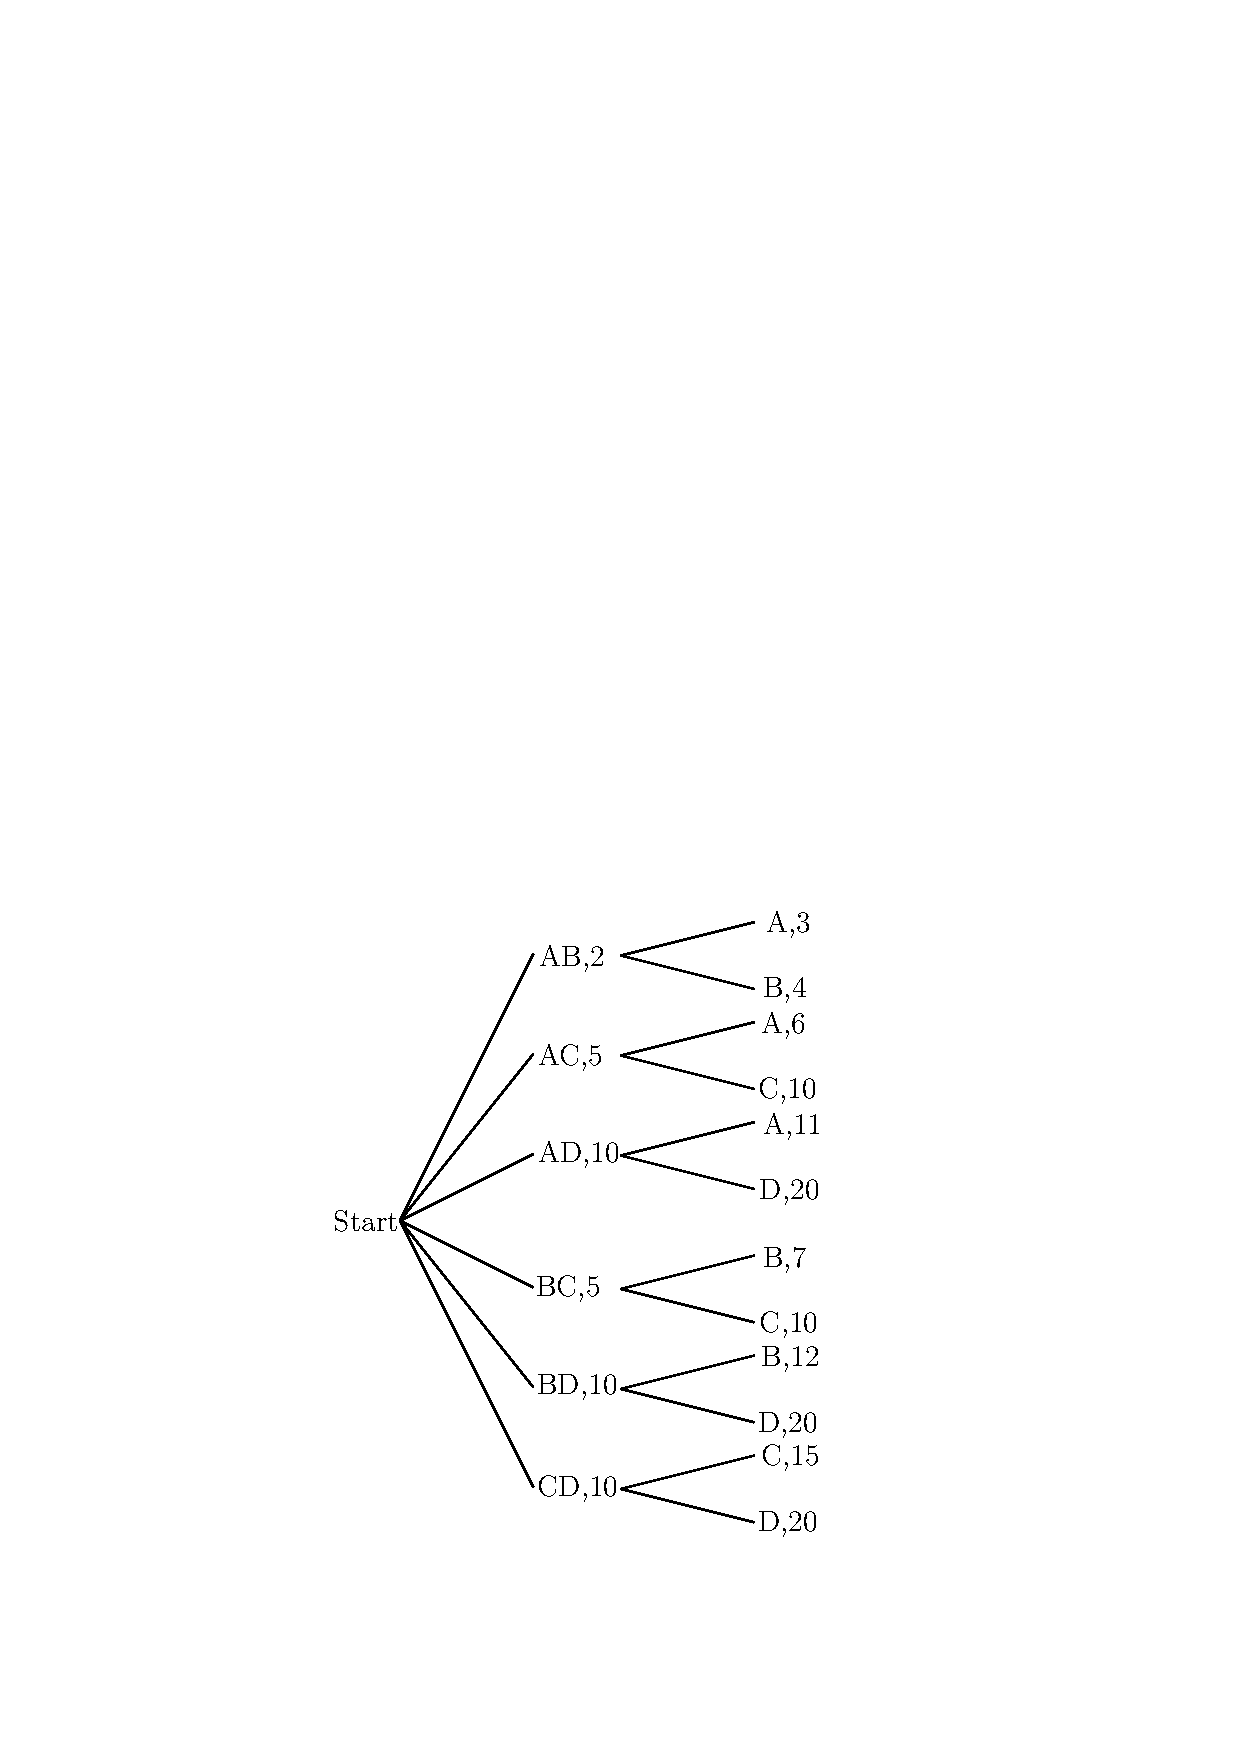
\includegraphics[width=1.8in]{images/returnTree.pdf}
\end{center}
\caption{Every possible return trip after the initial trip\\across the bridge including the time since Start.}\label{returnTree}
\end{minipage}
\end{figure}

% \begin{figure}[htb]
% \begin{center}
% \includegraphics[width=1.5in]{startTree.pdf}
% \end{center}
% \caption\Instr{  Every possible pair of people who could be the first to cross the bridge}\label{startTree}
% \end{figure}
% \renewcommand{\thefigure}{\arabic{chapter}.\arabic{figure}(\alph{bluefigure})} 
% % \setcounter{bluefigure}{1}
% \addtocounter{figure}{-1}
% \addtocounter{bluefigure}{1}
% \begin{figure}[htb]
% \begin{center}
% 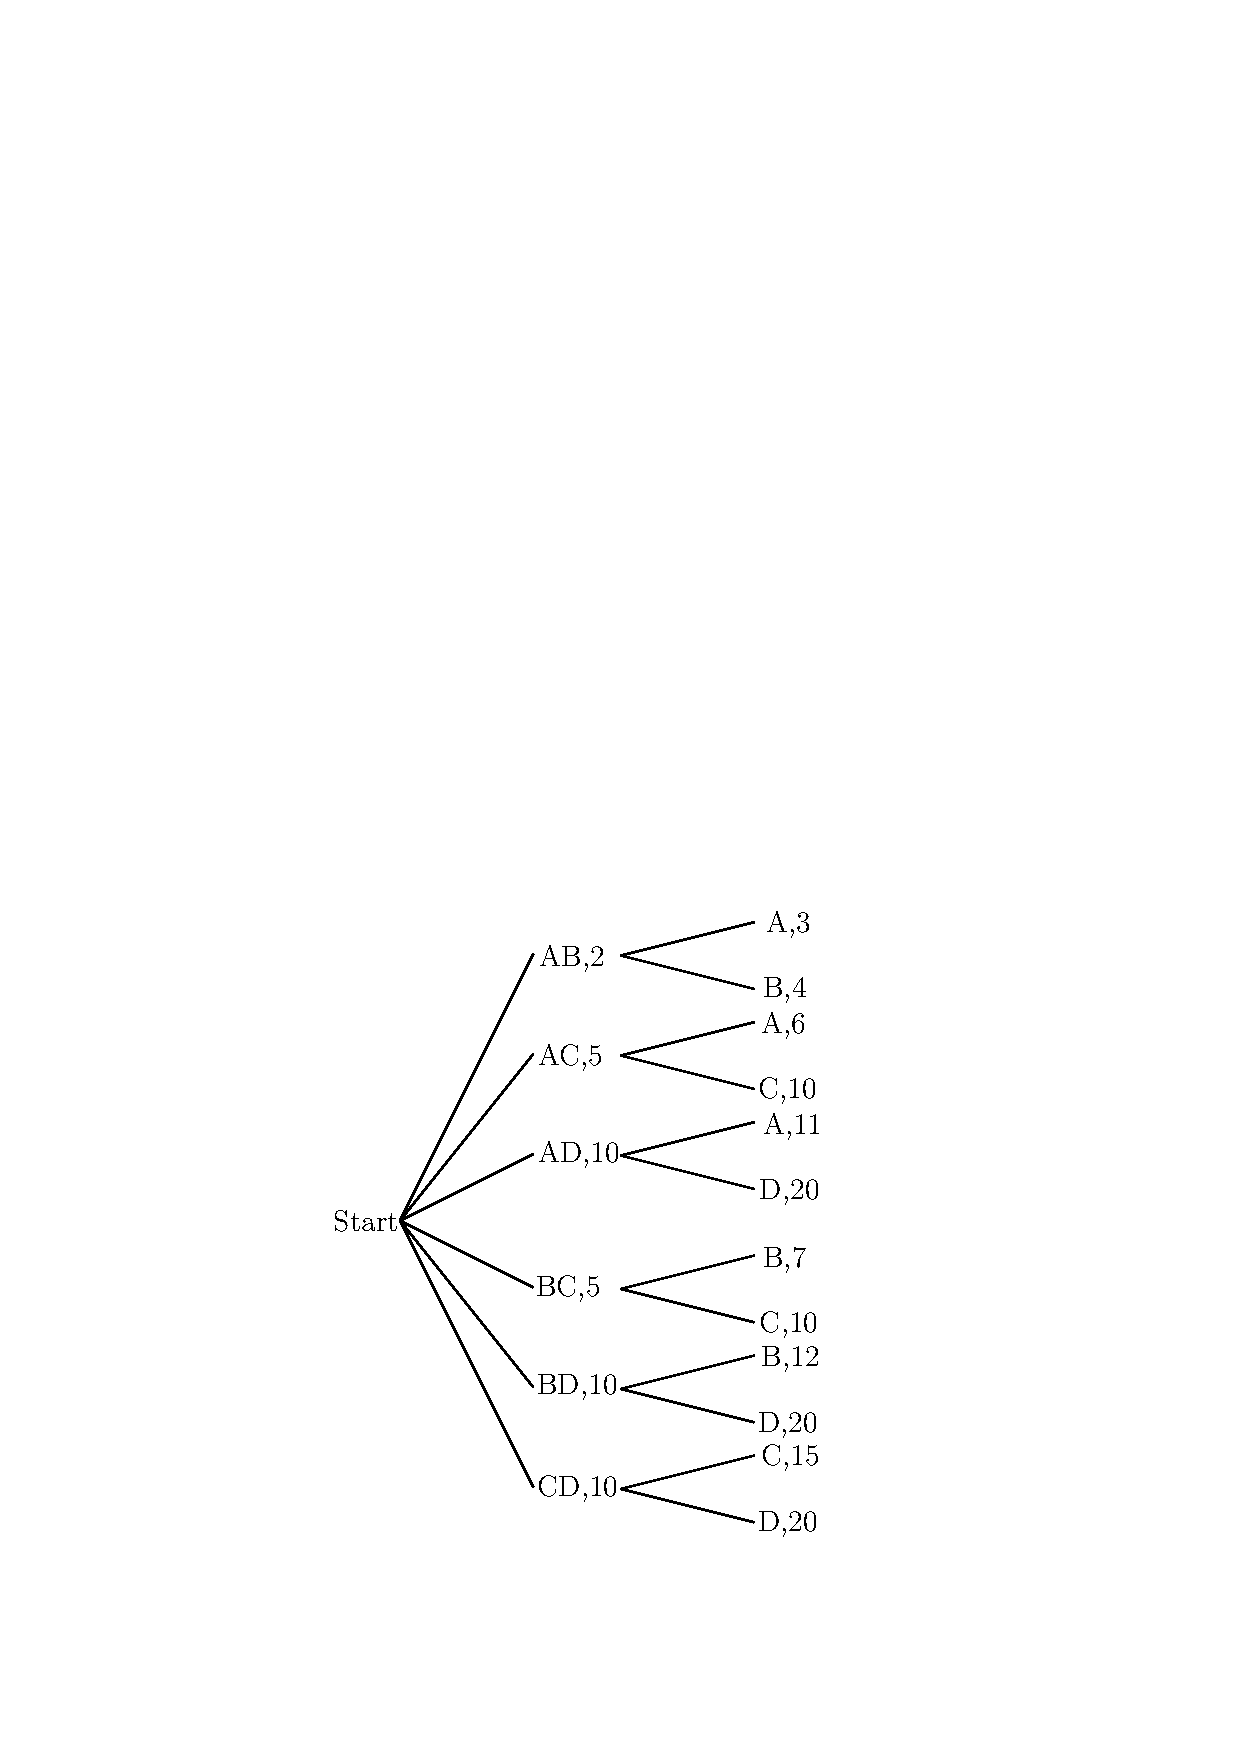
\includegraphics[width=2in]{images/returnTree.pdf}
% \end{center}
% \caption\Instr{  Every possible return trip after the initial trip across the bridge including the time since Start}\label{returnTree}
% \end{figure}

\renewcommand{\thefigure}{\arabic{chapter}.\arabic{figure}(\alph{bluefigure})} 
% \setcounter{bluefigure}{1}
\addtocounter{figure}{-1}
\addtocounter{bluefigure}{1}
\begin{figure}[htb]
\begin{center}
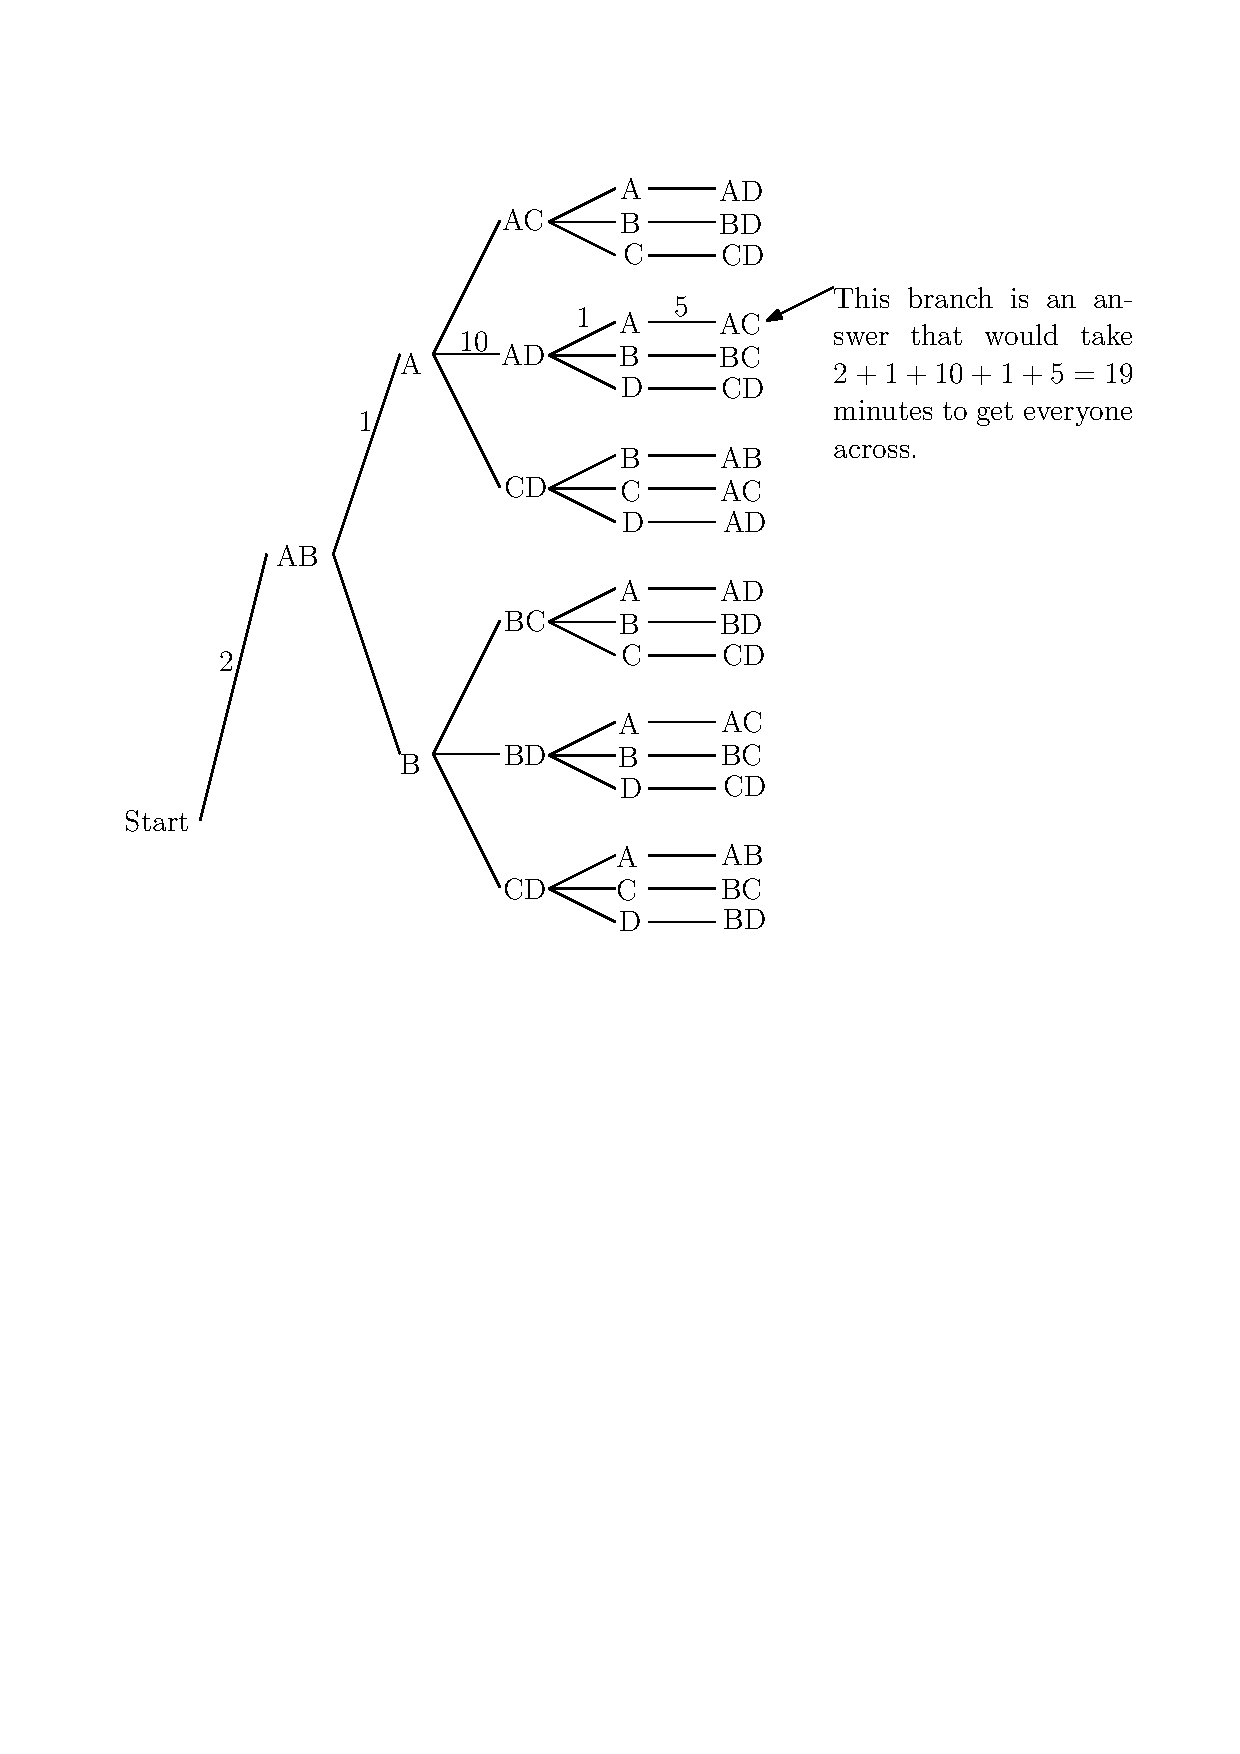
\includegraphics[width=3.4in]{images/alfredBruce.pdf}
\end{center}
\caption{ The entire solution tree for when Alfred and Bruce cross first}\label{alfredBruce}
\end{figure}

Students may want to keep a running total of the time taken along each branch as they construct the tree (see Figure~{\normalfont\ref{returnTree}}), or they may prefer to label each edge with the time. Then, if ever a branch reaches more than $17$ minutes (or whatever lowest total they have identified so far), they need not complete this branch since it cannot produce a faster time (this is called pruning the tree).
}

\wbvfill
%<*logicProblems:crossBridge:4minBruce>
\item\label{4minBruce} It turns out that Bruce stubbed his toe on the way to the bridge and will actually take $4$ minutes to cross the bridge. Now how long would it take for everyone to get across the bridge?
%</logicProblems:crossBridge:4minBruce>

\Instr{ If we use the optimal method discussed in Question~{\normalfont\ref{19min}} we find that it takes $23$ minutes for the party to cross the bridge. It is easy to see that we must replace each $2$ in the calculation of Question~{\normalfont\ref{19min}} with a $4$, and since Bruce crossed the bridge $3$ times this adds $6$ minutes to the total time. However, if we use the first method discussed where Alfred went across all five times and escorted each team member we notice Bruce only crossed the bridge once. Therefore we only need to add $2$ minutes to the total time in this method producing a total time of $21$ minutes. 

These two problems are carefully chosen to point out that just because a technique works well in one setting does not mean it is always going to be the best method to use.}

\wbvfill
%<*logicProblems:crossBridge:noQuicker>
\item  Why is there no quicker way to get everyone across in Question~{\normalfont\ref{4minBruce}}? Thoroughly explain your answer.
%</logicProblems:crossBridge:noQuicker>

\Instr{  Again we suggest using a tree diagram\index{tree diagram} to exhaust all possible methods to show which method is optimal. 
}

\wbvfill
%<*logicProblems:crossBridge:end>
\end{enumerate}
%</logicProblems:crossBridge:end>

\newpage
\section{Project Choices}
\begin{enumerate}
\item \textbf{Project Question:} How many different ways can you make \$50 in US bills? Provide a tree diagram to support your claim and write a statement about how you used results from the \$20 class activity to find your answer.
\par\Instr{ The problem using coins to make a dollar is widely known, and I can find an answer for making \$50 with change but that number is extremely high because of the use of coins. We are asking for much less and the answer doesn't seem to be immediately available on the net.
\par
There are 451:
\begin{longtable}[c]{|c|c|c|c|c|c||c|c|c|c|c|c|}
\hline
50s & 20s & 10s & 5s & 2s & 1s & 50s & 20s & 10s & 5s & 2s & 1s \\ \hline\hline
0 & 0 & 0 & 0 & 0 & 50 &
0 & 0 & 0 & 0 & 1 & 48 \\ \hline
0 & 0 & 0 & 0 & 2 & 46 &
0 & 0 & 0 & 0 & 3 & 44 \\ \hline
0 & 0 & 0 & 0 & 4 & 42 &
0 & 0 & 0 & 0 & 5 & 40 \\ \hline
0 & 0 & 0 & 0 & 6 & 38 &
0 & 0 & 0 & 0 & 7 & 36 \\ \hline
0 & 0 & 0 & 0 & 8 & 34 &
0 & 0 & 0 & 0 & 9 & 32 \\ \hline
0 & 0 & 0 & 0 & 10 & 30 &
0 & 0 & 0 & 0 & 11 & 28 \\ \hline
0 & 0 & 0 & 0 & 12 & 26 &
0 & 0 & 0 & 0 & 13 & 24 \\ \hline
0 & 0 & 0 & 0 & 14 & 22 &
0 & 0 & 0 & 0 & 15 & 20 \\ \hline
0 & 0 & 0 & 0 & 16 & 18 &
0 & 0 & 0 & 0 & 17 & 16 \\ \hline
0 & 0 & 0 & 0 & 18 & 14 &
0 & 0 & 0 & 0 & 19 & 12 \\ \hline
0 & 0 & 0 & 0 & 20 & 10 &
0 & 0 & 0 & 0 & 21 & 8 \\ \hline
0 & 0 & 0 & 0 & 22 & 6 &
0 & 0 & 0 & 0 & 23 & 4 \\ \hline
0 & 0 & 0 & 0 & 24 & 2 &
0 & 0 & 0 & 0 & 25 & 0 \\ \hline
0 & 0 & 0 & 1 & 0 & 45 &
0 & 0 & 0 & 1 & 1 & 43 \\ \hline
0 & 0 & 0 & 1 & 2 & 41 &
0 & 0 & 0 & 1 & 3 & 39 \\ \hline
0 & 0 & 0 & 1 & 4 & 37 &
0 & 0 & 0 & 1 & 5 & 35 \\ \hline
0 & 0 & 0 & 1 & 6 & 33 &
0 & 0 & 0 & 1 & 7 & 31 \\ \hline
0 & 0 & 0 & 1 & 8 & 29 &
0 & 0 & 0 & 1 & 9 & 27 \\ \hline
0 & 0 & 0 & 1 & 10 & 25 &
0 & 0 & 0 & 1 & 11 & 23 \\ \hline
0 & 0 & 0 & 1 & 12 & 21 &
0 & 0 & 0 & 1 & 13 & 19 \\ \hline
0 & 0 & 0 & 1 & 14 & 17 &
0 & 0 & 0 & 1 & 15 & 15 \\ \hline
0 & 0 & 0 & 1 & 16 & 13 &
0 & 0 & 0 & 1 & 17 & 11 \\ \hline
0 & 0 & 0 & 1 & 18 & 9 &
0 & 0 & 0 & 1 & 19 & 7 \\ \hline
0 & 0 & 0 & 1 & 20 & 5 &
0 & 0 & 0 & 1 & 21 & 3 \\ \hline
0 & 0 & 0 & 1 & 22 & 1 &
0 & 0 & 0 & 2 & 0 & 40 \\ \hline
0 & 0 & 0 & 2 & 1 & 38 &
0 & 0 & 0 & 2 & 2 & 36 \\ \hline
0 & 0 & 0 & 2 & 3 & 34 &
0 & 0 & 0 & 2 & 4 & 32 \\ \hline
0 & 0 & 0 & 2 & 5 & 30 &
0 & 0 & 0 & 2 & 6 & 28 \\ \hline
0 & 0 & 0 & 2 & 7 & 26 &
0 & 0 & 0 & 2 & 8 & 24 \\ \hline
0 & 0 & 0 & 2 & 9 & 22 &
0 & 0 & 0 & 2 & 10 & 20 \\ \hline
0 & 0 & 0 & 2 & 11 & 18 &
0 & 0 & 0 & 2 & 12 & 16 \\ \hline
0 & 0 & 0 & 2 & 13 & 14 &
0 & 0 & 0 & 2 & 14 & 12 \\ \hline
0 & 0 & 0 & 2 & 15 & 10 &
0 & 0 & 0 & 2 & 16 & 8 \\ \hline
0 & 0 & 0 & 2 & 17 & 6 &
0 & 0 & 0 & 2 & 18 & 4 \\ \hline
0 & 0 & 0 & 2 & 19 & 2 &
0 & 0 & 0 & 2 & 20 & 0 \\ \hline
0 & 0 & 0 & 3 & 0 & 35 &
0 & 0 & 0 & 3 & 1 & 33 \\ \hline
0 & 0 & 0 & 3 & 2 & 31 &
0 & 0 & 0 & 3 & 3 & 29 \\ \hline
0 & 0 & 0 & 3 & 4 & 27 &
0 & 0 & 0 & 3 & 5 & 25 \\ \hline
0 & 0 & 0 & 3 & 6 & 23 &
0 & 0 & 0 & 3 & 7 & 21 \\ \hline
0 & 0 & 0 & 3 & 8 & 19 &
0 & 0 & 0 & 3 & 9 & 17 \\ \hline
0 & 0 & 0 & 3 & 10 & 15 &
0 & 0 & 0 & 3 & 11 & 13 \\ \hline
0 & 0 & 0 & 3 & 12 & 11 &
0 & 0 & 0 & 3 & 13 & 9 \\ \hline
0 & 0 & 0 & 3 & 14 & 7 &
0 & 0 & 0 & 3 & 15 & 5 \\ \hline
0 & 0 & 0 & 3 & 16 & 3 &
0 & 0 & 0 & 3 & 17 & 1 \\ \hline
0 & 0 & 0 & 4 & 0 & 30 &
0 & 0 & 0 & 4 & 1 & 28 \\ \hline
0 & 0 & 0 & 4 & 2 & 26 &
0 & 0 & 0 & 4 & 3 & 24 \\ \hline
0 & 0 & 0 & 4 & 4 & 22 &
0 & 0 & 0 & 4 & 5 & 20 \\ \hline
0 & 0 & 0 & 4 & 6 & 18 &
0 & 0 & 0 & 4 & 7 & 16 \\ \hline
0 & 0 & 0 & 4 & 8 & 14 &
0 & 0 & 0 & 4 & 9 & 12 \\ \hline
0 & 0 & 0 & 4 & 10 & 10 &
0 & 0 & 0 & 4 & 11 & 8 \\ \hline
0 & 0 & 0 & 4 & 12 & 6 &
0 & 0 & 0 & 4 & 13 & 4 \\ \hline
0 & 0 & 0 & 4 & 14 & 2 &
0 & 0 & 0 & 4 & 15 & 0 \\ \hline
0 & 0 & 0 & 5 & 0 & 25 &
0 & 0 & 0 & 5 & 1 & 23 \\ \hline
0 & 0 & 0 & 5 & 2 & 21 &
0 & 0 & 0 & 5 & 3 & 19 \\ \hline
0 & 0 & 0 & 5 & 4 & 17 &
0 & 0 & 0 & 5 & 5 & 15 \\ \hline
0 & 0 & 0 & 5 & 6 & 13 &
0 & 0 & 0 & 5 & 7 & 11 \\ \hline
0 & 0 & 0 & 5 & 8 & 9 &
0 & 0 & 0 & 5 & 9 & 7 \\ \hline
0 & 0 & 0 & 5 & 10 & 5 &
0 & 0 & 0 & 5 & 11 & 3 \\ \hline
0 & 0 & 0 & 5 & 12 & 1 &
0 & 0 & 0 & 6 & 0 & 20 \\ \hline
0 & 0 & 0 & 6 & 1 & 18 &
0 & 0 & 0 & 6 & 2 & 16 \\ \hline
0 & 0 & 0 & 6 & 3 & 14 &
0 & 0 & 0 & 6 & 4 & 12 \\ \hline
0 & 0 & 0 & 6 & 5 & 10 &
0 & 0 & 0 & 6 & 6 & 8 \\ \hline
0 & 0 & 0 & 6 & 7 & 6 &
0 & 0 & 0 & 6 & 8 & 4 \\ \hline
0 & 0 & 0 & 6 & 9 & 2 &
0 & 0 & 0 & 6 & 10 & 0 \\ \hline
0 & 0 & 0 & 7 & 0 & 15 &
0 & 0 & 0 & 7 & 1 & 13 \\ \hline
0 & 0 & 0 & 7 & 2 & 11 &
0 & 0 & 0 & 7 & 3 & 9 \\ \hline
0 & 0 & 0 & 7 & 4 & 7 &
0 & 0 & 0 & 7 & 5 & 5 \\ \hline
0 & 0 & 0 & 7 & 6 & 3 &
0 & 0 & 0 & 7 & 7 & 1 \\ \hline
0 & 0 & 0 & 8 & 0 & 10 &
0 & 0 & 0 & 8 & 1 & 8 \\ \hline
0 & 0 & 0 & 8 & 2 & 6 &
0 & 0 & 0 & 8 & 3 & 4 \\ \hline
0 & 0 & 0 & 8 & 4 & 2 &
0 & 0 & 0 & 8 & 5 & 0 \\ \hline
0 & 0 & 0 & 9 & 0 & 5 &
0 & 0 & 0 & 9 & 1 & 3 \\ \hline
0 & 0 & 0 & 9 & 2 & 1 &
0 & 0 & 0 & 10 & 0 & 0 \\ \hline
0 & 0 & 1 & 0 & 0 & 40 &
0 & 0 & 1 & 0 & 1 & 38 \\ \hline
0 & 0 & 1 & 0 & 2 & 36 &
0 & 0 & 1 & 0 & 3 & 34 \\ \hline
0 & 0 & 1 & 0 & 4 & 32 &
0 & 0 & 1 & 0 & 5 & 30 \\ \hline
0 & 0 & 1 & 0 & 6 & 28 &
0 & 0 & 1 & 0 & 7 & 26 \\ \hline
0 & 0 & 1 & 0 & 8 & 24 &
0 & 0 & 1 & 0 & 9 & 22 \\ \hline
0 & 0 & 1 & 0 & 10 & 20 &
0 & 0 & 1 & 0 & 11 & 18 \\ \hline
0 & 0 & 1 & 0 & 12 & 16 &
0 & 0 & 1 & 0 & 13 & 14 \\ \hline
0 & 0 & 1 & 0 & 14 & 12 &
0 & 0 & 1 & 0 & 15 & 10 \\ \hline
0 & 0 & 1 & 0 & 16 & 8 &
0 & 0 & 1 & 0 & 17 & 6 \\ \hline
0 & 0 & 1 & 0 & 18 & 4 &
0 & 0 & 1 & 0 & 19 & 2 \\ \hline
0 & 0 & 1 & 0 & 20 & 0 &
0 & 0 & 1 & 1 & 0 & 35 \\ \hline
0 & 0 & 1 & 1 & 1 & 33 &
0 & 0 & 1 & 1 & 2 & 31 \\ \hline
0 & 0 & 1 & 1 & 3 & 29 &
0 & 0 & 1 & 1 & 4 & 27 \\ \hline
0 & 0 & 1 & 1 & 5 & 25 &
0 & 0 & 1 & 1 & 6 & 23 \\ \hline
0 & 0 & 1 & 1 & 7 & 21 &
0 & 0 & 1 & 1 & 8 & 19 \\ \hline
0 & 0 & 1 & 1 & 9 & 17 &
0 & 0 & 1 & 1 & 10 & 15 \\ \hline
0 & 0 & 1 & 1 & 11 & 13 &
0 & 0 & 1 & 1 & 12 & 11 \\ \hline
0 & 0 & 1 & 1 & 13 & 9 &
0 & 0 & 1 & 1 & 14 & 7 \\ \hline
0 & 0 & 1 & 1 & 15 & 5 &
0 & 0 & 1 & 1 & 16 & 3 \\ \hline
0 & 0 & 1 & 1 & 17 & 1 &
0 & 0 & 1 & 2 & 0 & 30 \\ \hline
0 & 0 & 1 & 2 & 1 & 28 &
0 & 0 & 1 & 2 & 2 & 26 \\ \hline
0 & 0 & 1 & 2 & 3 & 24 &
0 & 0 & 1 & 2 & 4 & 22 \\ \hline
0 & 0 & 1 & 2 & 5 & 20 &
0 & 0 & 1 & 2 & 6 & 18 \\ \hline
0 & 0 & 1 & 2 & 7 & 16 &
0 & 0 & 1 & 2 & 8 & 14 \\ \hline
0 & 0 & 1 & 2 & 9 & 12 &
0 & 0 & 1 & 2 & 10 & 10 \\ \hline
0 & 0 & 1 & 2 & 11 & 8 &
0 & 0 & 1 & 2 & 12 & 6 \\ \hline
0 & 0 & 1 & 2 & 13 & 4 &
0 & 0 & 1 & 2 & 14 & 2 \\ \hline
0 & 0 & 1 & 2 & 15 & 0 &
0 & 0 & 1 & 3 & 0 & 25 \\ \hline
0 & 0 & 1 & 3 & 1 & 23 &
0 & 0 & 1 & 3 & 2 & 21 \\ \hline
0 & 0 & 1 & 3 & 3 & 19 &
0 & 0 & 1 & 3 & 4 & 17 \\ \hline
0 & 0 & 1 & 3 & 5 & 15 &
0 & 0 & 1 & 3 & 6 & 13 \\ \hline
0 & 0 & 1 & 3 & 7 & 11 &
0 & 0 & 1 & 3 & 8 & 9 \\ \hline
0 & 0 & 1 & 3 & 9 & 7 &
0 & 0 & 1 & 3 & 10 & 5 \\ \hline
0 & 0 & 1 & 3 & 11 & 3 &
0 & 0 & 1 & 3 & 12 & 1 \\ \hline
0 & 0 & 1 & 4 & 0 & 20 &
0 & 0 & 1 & 4 & 1 & 18 \\ \hline
0 & 0 & 1 & 4 & 2 & 16 &
0 & 0 & 1 & 4 & 3 & 14 \\ \hline
0 & 0 & 1 & 4 & 4 & 12 &
0 & 0 & 1 & 4 & 5 & 10 \\ \hline
0 & 0 & 1 & 4 & 6 & 8 &
0 & 0 & 1 & 4 & 7 & 6 \\ \hline
0 & 0 & 1 & 4 & 8 & 4 &
0 & 0 & 1 & 4 & 9 & 2 \\ \hline
0 & 0 & 1 & 4 & 10 & 0 &
0 & 0 & 1 & 5 & 0 & 15 \\ \hline
0 & 0 & 1 & 5 & 1 & 13 &
0 & 0 & 1 & 5 & 2 & 11 \\ \hline
0 & 0 & 1 & 5 & 3 & 9 &
0 & 0 & 1 & 5 & 4 & 7 \\ \hline
0 & 0 & 1 & 5 & 5 & 5 &
0 & 0 & 1 & 5 & 6 & 3 \\ \hline
0 & 0 & 1 & 5 & 7 & 1 &
0 & 0 & 1 & 6 & 0 & 10 \\ \hline
0 & 0 & 1 & 6 & 1 & 8 &
0 & 0 & 1 & 6 & 2 & 6 \\ \hline
0 & 0 & 1 & 6 & 3 & 4 &
0 & 0 & 1 & 6 & 4 & 2 \\ \hline
0 & 0 & 1 & 6 & 5 & 0 &
0 & 0 & 1 & 7 & 0 & 5 \\ \hline
0 & 0 & 1 & 7 & 1 & 3 &
0 & 0 & 1 & 7 & 2 & 1 \\ \hline
0 & 0 & 1 & 8 & 0 & 0 &
0 & 0 & 2 & 0 & 0 & 30 \\ \hline
0 & 0 & 2 & 0 & 1 & 28 &
0 & 0 & 2 & 0 & 2 & 26 \\ \hline
0 & 0 & 2 & 0 & 3 & 24 &
0 & 0 & 2 & 0 & 4 & 22 \\ \hline
0 & 0 & 2 & 0 & 5 & 20 &
0 & 0 & 2 & 0 & 6 & 18 \\ \hline
0 & 0 & 2 & 0 & 7 & 16 &
0 & 0 & 2 & 0 & 8 & 14 \\ \hline
0 & 0 & 2 & 0 & 9 & 12 &
0 & 0 & 2 & 0 & 10 & 10 \\ \hline
0 & 0 & 2 & 0 & 11 & 8 &
0 & 0 & 2 & 0 & 12 & 6 \\ \hline
0 & 0 & 2 & 0 & 13 & 4 &
0 & 0 & 2 & 0 & 14 & 2 \\ \hline
0 & 0 & 2 & 0 & 15 & 0 &
0 & 0 & 2 & 1 & 0 & 25 \\ \hline
0 & 0 & 2 & 1 & 1 & 23 &
0 & 0 & 2 & 1 & 2 & 21 \\ \hline
0 & 0 & 2 & 1 & 3 & 19 &
0 & 0 & 2 & 1 & 4 & 17 \\ \hline
0 & 0 & 2 & 1 & 5 & 15 &
0 & 0 & 2 & 1 & 6 & 13 \\ \hline
0 & 0 & 2 & 1 & 7 & 11 &
0 & 0 & 2 & 1 & 8 & 9 \\ \hline
0 & 0 & 2 & 1 & 9 & 7 &
0 & 0 & 2 & 1 & 10 & 5 \\ \hline
0 & 0 & 2 & 1 & 11 & 3 &
0 & 0 & 2 & 1 & 12 & 1 \\ \hline
0 & 0 & 2 & 2 & 0 & 20 &
0 & 0 & 2 & 2 & 1 & 18 \\ \hline
0 & 0 & 2 & 2 & 2 & 16 &
0 & 0 & 2 & 2 & 3 & 14 \\ \hline
0 & 0 & 2 & 2 & 4 & 12 &
0 & 0 & 2 & 2 & 5 & 10 \\ \hline
0 & 0 & 2 & 2 & 6 & 8 &
0 & 0 & 2 & 2 & 7 & 6 \\ \hline
0 & 0 & 2 & 2 & 8 & 4 &
0 & 0 & 2 & 2 & 9 & 2 \\ \hline
0 & 0 & 2 & 2 & 10 & 0 &
0 & 0 & 2 & 3 & 0 & 15 \\ \hline
0 & 0 & 2 & 3 & 1 & 13 &
0 & 0 & 2 & 3 & 2 & 11 \\ \hline
0 & 0 & 2 & 3 & 3 & 9 &
0 & 0 & 2 & 3 & 4 & 7 \\ \hline
0 & 0 & 2 & 3 & 5 & 5 &
0 & 0 & 2 & 3 & 6 & 3 \\ \hline
0 & 0 & 2 & 3 & 7 & 1 &
0 & 0 & 2 & 4 & 0 & 10 \\ \hline
0 & 0 & 2 & 4 & 1 & 8 &
0 & 0 & 2 & 4 & 2 & 6 \\ \hline
0 & 0 & 2 & 4 & 3 & 4 &
0 & 0 & 2 & 4 & 4 & 2 \\ \hline
0 & 0 & 2 & 4 & 5 & 0 &
0 & 0 & 2 & 5 & 0 & 5 \\ \hline
0 & 0 & 2 & 5 & 1 & 3 &
0 & 0 & 2 & 5 & 2 & 1 \\ \hline
0 & 0 & 2 & 6 & 0 & 0 &
0 & 0 & 3 & 0 & 0 & 20 \\ \hline
0 & 0 & 3 & 0 & 1 & 18 &
0 & 0 & 3 & 0 & 2 & 16 \\ \hline
0 & 0 & 3 & 0 & 3 & 14 &
0 & 0 & 3 & 0 & 4 & 12 \\ \hline
0 & 0 & 3 & 0 & 5 & 10 &
0 & 0 & 3 & 0 & 6 & 8 \\ \hline
0 & 0 & 3 & 0 & 7 & 6 &
0 & 0 & 3 & 0 & 8 & 4 \\ \hline
0 & 0 & 3 & 0 & 9 & 2 &
0 & 0 & 3 & 0 & 10 & 0 \\ \hline
0 & 0 & 3 & 1 & 0 & 15 &
0 & 0 & 3 & 1 & 1 & 13 \\ \hline
0 & 0 & 3 & 1 & 2 & 11 &
0 & 0 & 3 & 1 & 3 & 9 \\ \hline
0 & 0 & 3 & 1 & 4 & 7 &
0 & 0 & 3 & 1 & 5 & 5 \\ \hline
0 & 0 & 3 & 1 & 6 & 3 &
0 & 0 & 3 & 1 & 7 & 1 \\ \hline
0 & 0 & 3 & 2 & 0 & 10 &
0 & 0 & 3 & 2 & 1 & 8 \\ \hline
0 & 0 & 3 & 2 & 2 & 6 &
0 & 0 & 3 & 2 & 3 & 4 \\ \hline
0 & 0 & 3 & 2 & 4 & 2 &
0 & 0 & 3 & 2 & 5 & 0 \\ \hline
0 & 0 & 3 & 3 & 0 & 5 &
0 & 0 & 3 & 3 & 1 & 3 \\ \hline
0 & 0 & 3 & 3 & 2 & 1 &
0 & 0 & 3 & 4 & 0 & 0 \\ \hline
0 & 0 & 4 & 0 & 0 & 10 &
0 & 0 & 4 & 0 & 1 & 8 \\ \hline
0 & 0 & 4 & 0 & 2 & 6 &
0 & 0 & 4 & 0 & 3 & 4 \\ \hline
0 & 0 & 4 & 0 & 4 & 2 &
0 & 0 & 4 & 0 & 5 & 0 \\ \hline
0 & 0 & 4 & 1 & 0 & 5 &
0 & 0 & 4 & 1 & 1 & 3 \\ \hline
0 & 0 & 4 & 1 & 2 & 1 &
0 & 0 & 4 & 2 & 0 & 0 \\ \hline
0 & 0 & 5 & 0 & 0 & 0 &
0 & 1 & 0 & 0 & 0 & 30 \\ \hline
0 & 1 & 0 & 0 & 1 & 28 &
0 & 1 & 0 & 0 & 2 & 26 \\ \hline
0 & 1 & 0 & 0 & 3 & 24 &
0 & 1 & 0 & 0 & 4 & 22 \\ \hline
0 & 1 & 0 & 0 & 5 & 20 &
0 & 1 & 0 & 0 & 6 & 18 \\ \hline
0 & 1 & 0 & 0 & 7 & 16 &
0 & 1 & 0 & 0 & 8 & 14 \\ \hline
0 & 1 & 0 & 0 & 9 & 12 &
0 & 1 & 0 & 0 & 10 & 10 \\ \hline
0 & 1 & 0 & 0 & 11 & 8 &
0 & 1 & 0 & 0 & 12 & 6 \\ \hline
0 & 1 & 0 & 0 & 13 & 4 &
0 & 1 & 0 & 0 & 14 & 2 \\ \hline
0 & 1 & 0 & 0 & 15 & 0 &
0 & 1 & 0 & 1 & 0 & 25 \\ \hline
0 & 1 & 0 & 1 & 1 & 23 &
0 & 1 & 0 & 1 & 2 & 21 \\ \hline
0 & 1 & 0 & 1 & 3 & 19 &
0 & 1 & 0 & 1 & 4 & 17 \\ \hline
0 & 1 & 0 & 1 & 5 & 15 &
0 & 1 & 0 & 1 & 6 & 13 \\ \hline
0 & 1 & 0 & 1 & 7 & 11 &
0 & 1 & 0 & 1 & 8 & 9 \\ \hline
0 & 1 & 0 & 1 & 9 & 7 &
0 & 1 & 0 & 1 & 10 & 5 \\ \hline
0 & 1 & 0 & 1 & 11 & 3 &
0 & 1 & 0 & 1 & 12 & 1 \\ \hline
0 & 1 & 0 & 2 & 0 & 20 &
0 & 1 & 0 & 2 & 1 & 18 \\ \hline
0 & 1 & 0 & 2 & 2 & 16 &
0 & 1 & 0 & 2 & 3 & 14 \\ \hline
0 & 1 & 0 & 2 & 4 & 12 &
0 & 1 & 0 & 2 & 5 & 10 \\ \hline
0 & 1 & 0 & 2 & 6 & 8 &
0 & 1 & 0 & 2 & 7 & 6 \\ \hline
0 & 1 & 0 & 2 & 8 & 4 &
0 & 1 & 0 & 2 & 9 & 2 \\ \hline
0 & 1 & 0 & 2 & 10 & 0 &
0 & 1 & 0 & 3 & 0 & 15 \\ \hline
0 & 1 & 0 & 3 & 1 & 13 &
0 & 1 & 0 & 3 & 2 & 11 \\ \hline
0 & 1 & 0 & 3 & 3 & 9 &
0 & 1 & 0 & 3 & 4 & 7 \\ \hline
0 & 1 & 0 & 3 & 5 & 5 &
0 & 1 & 0 & 3 & 6 & 3 \\ \hline
0 & 1 & 0 & 3 & 7 & 1 &
0 & 1 & 0 & 4 & 0 & 10 \\ \hline
0 & 1 & 0 & 4 & 1 & 8 &
0 & 1 & 0 & 4 & 2 & 6 \\ \hline
0 & 1 & 0 & 4 & 3 & 4 &
0 & 1 & 0 & 4 & 4 & 2 \\ \hline
0 & 1 & 0 & 4 & 5 & 0 &
0 & 1 & 0 & 5 & 0 & 5 \\ \hline
0 & 1 & 0 & 5 & 1 & 3 &
0 & 1 & 0 & 5 & 2 & 1 \\ \hline
0 & 1 & 0 & 6 & 0 & 0 &
0 & 1 & 1 & 0 & 0 & 20 \\ \hline
0 & 1 & 1 & 0 & 1 & 18 &
0 & 1 & 1 & 0 & 2 & 16 \\ \hline
0 & 1 & 1 & 0 & 3 & 14 &
0 & 1 & 1 & 0 & 4 & 12 \\ \hline
0 & 1 & 1 & 0 & 5 & 10 &
0 & 1 & 1 & 0 & 6 & 8 \\ \hline
0 & 1 & 1 & 0 & 7 & 6 &
0 & 1 & 1 & 0 & 8 & 4 \\ \hline
0 & 1 & 1 & 0 & 9 & 2 &
0 & 1 & 1 & 0 & 10 & 0 \\ \hline
0 & 1 & 1 & 1 & 0 & 15 &
0 & 1 & 1 & 1 & 1 & 13 \\ \hline
0 & 1 & 1 & 1 & 2 & 11 &
0 & 1 & 1 & 1 & 3 & 9 \\ \hline
0 & 1 & 1 & 1 & 4 & 7 &
0 & 1 & 1 & 1 & 5 & 5 \\ \hline
0 & 1 & 1 & 1 & 6 & 3 &
0 & 1 & 1 & 1 & 7 & 1 \\ \hline
0 & 1 & 1 & 2 & 0 & 10 &
0 & 1 & 1 & 2 & 1 & 8 \\ \hline
0 & 1 & 1 & 2 & 2 & 6 &
0 & 1 & 1 & 2 & 3 & 4 \\ \hline
0 & 1 & 1 & 2 & 4 & 2 &
0 & 1 & 1 & 2 & 5 & 0 \\ \hline
0 & 1 & 1 & 3 & 0 & 5 &
0 & 1 & 1 & 3 & 1 & 3 \\ \hline
0 & 1 & 1 & 3 & 2 & 1 &
0 & 1 & 1 & 4 & 0 & 0 \\ \hline
0 & 1 & 2 & 0 & 0 & 10 &
0 & 1 & 2 & 0 & 1 & 8 \\ \hline
0 & 1 & 2 & 0 & 2 & 6 &
0 & 1 & 2 & 0 & 3 & 4 \\ \hline
0 & 1 & 2 & 0 & 4 & 2 &
0 & 1 & 2 & 0 & 5 & 0 \\ \hline
0 & 1 & 2 & 1 & 0 & 5 &
0 & 1 & 2 & 1 & 1 & 3 \\ \hline
0 & 1 & 2 & 1 & 2 & 1 &
0 & 1 & 2 & 2 & 0 & 0 \\ \hline
0 & 1 & 3 & 0 & 0 & 0 &
0 & 2 & 0 & 0 & 0 & 10 \\ \hline
0 & 2 & 0 & 0 & 1 & 8 &
0 & 2 & 0 & 0 & 2 & 6 \\ \hline
0 & 2 & 0 & 0 & 3 & 4 &
0 & 2 & 0 & 0 & 4 & 2 \\ \hline
0 & 2 & 0 & 0 & 5 & 0 &
0 & 2 & 0 & 1 & 0 & 5 \\ \hline
0 & 2 & 0 & 1 & 1 & 3 &
0 & 2 & 0 & 1 & 2 & 1 \\ \hline
0 & 2 & 0 & 2 & 0 & 0 &
0 & 2 & 1 & 0 & 0 & 0 \\ \hline
1 & 0 & 0 & 0 & 0 & 0 \\ \hline
\end{longtable}
}
\wbvfill

\item You need to cross a river in a small rowboat and take your possessions with you.  The boat is only big enough for you and one possession at a time.  Unfortunately, some of your belongings can't be left alone on the river bank while you transport the other.  Your belongings are: a wolf, a goat, and a big bag of cabbage.   Problems: the wolf will eat the goat and the goat will eat the cabbages if they are able to do so.  How do you get everything across?

\wbvfill

\end{enumerate}

\newpage
\section{Additional Exercises}
\begin{enumerate}
    \item You're at a meeting where there is a make-your-own-sandwich platter. There is only one kind of bread, but there is a choice of what to put on it. There are three different lunch meats, two different cheeses, and extras—mustard, mayonnaise, and lettuce—to choose from. How many sandwiches can you make using one lunch meat, one cheese and any combination of extras?
    \par\Instr{ Though this question can be answered using the multiplication principle, as in $3\times 2\times 2\times 2\times 2=48$, it is expected students will create a tree diagram. You may wish to use this exercise in class to give students an example of a tree diagram not associated with counting money.}
    \item How many different ways can you have \$30 in US bills? Make sure to utilize the techniques and strategies you have learned above and pay close attention to work from above that you may be able to re-use.
    \par\Instr{ One may initially think that you can multiply the number of ways ot make \$10 by the number of ways to make \$20. However that drastically over counts the possibilities because the tree diagram resulting from this method would not produce unique branches.
    \par
    So without some advance counting techniques we will need to use an exhaustive counting method. However we will utilize some information we already have produced above.
    \par
    We will partition the solution set into those that have a \$20 bill and those that do not. For those that do have a \$20 bill, we know that we need ten more dollars and so the \$20 bill with all the solutions from question \ref{making10} will produce all 11 of the collections of bills containing a \$20 bill that add to \$30. 
    \par
    The harder part is to find the collection of bills that do not contain a \$20 bill. There are many ways to do this, but we would suggest partitioning this work into those that contain a \$10 bill and those that do not. For those that do, we know there is a \$10 bill so there are \$20 left to account for. Without using a \$20 bill there are 40 ways to make \$20, as we have seen. It is only left to find how many ways there are to make \$30 using only fives, twos, and ones. Making a tree diagram for these collections reveals 58 possibilities.
    \par
    Finally we would add all the possibilities from above to get $11+40+58 = 109$ total collections of U.S. bills that make \$30.}
\end{enumerate}


%<*TruthTablesandLogic.Title>
\chapter{Logic}\label{truthTables}
%</TruthTablesandLogic.Title>
\setcounter{section}{-1}
\section{Mathematical Outcome}

%<*logic.mathOut2>
One fundamental concept of mathematics is logic. Sound mathematics comes from the ability to state definitively whether something is true or false. In order to explore mathematics from a theoretical standpoint one must first understand the basics of logic. This chapter uses students previous and intuitive knowledge to formally develop the concepts and terminology which will be used in developing conjectures and theorems throughout the text.

\begin{definition}
 A declarative statement (either verbally or written) which can be judged as either true or false (but never both) is known as a \textbf{statement}\index{statement}. 
 Determining a statement to be true or false is called the statement's truth value.
\end{definition}

Generally there are two types of statements. The first is called a \textbf{simple statement}\index{statement!simple} which only contains one idea, which we will denote using letters throughout this chapter. The second is the idea of combining a number of simple statements with conjunctions which form \textbf{compound statements}\index{statement!compound}. You will see compound statements in written and symbolic form which use connections such as ``and'' and ``or'' along with others. The concepts of logic follow from being able to consider the truth value of the simple statements and conclude the truth value of a compound statement.

The two most common and basic conjunctions used to form compound statements are ``and'' and ``or.'' Both of these conjunctions are explored in Activity~{\normalfont\ref{andor}} from an intuitive approach. 

The ``and'' conjunction is usually the most intuitive and students easily realize the only time when the statement constructed by adjoining two statements (either simple or compound) with an ``and'' is true is if both of the statements being adjoined are true, otherwise the compound statement is false.

Conversely, the ``or'' conjunction is often used in common vernacular to mean only one of the adjoined statements is true. For example when you ask a child ``Would you like chocolate \textbf{or} vanilla ice cream?'' you are not intending for them to choose both; you are simply giving them an option of choosing either. In logic however the conjunction ``or'' is evaluated as determining if at least one of the adjoining statements is true. Therefore we will determine that the compound statement adjoined by an ``or'' is true whenever one or both of the adjoined statements is true, hence it will only be false if both of the adjoined statements are false.

\begin{definition}
A tabular format for displaying all possible outcome combinations of a compound statement is known as a \textbf{truth table}\index{truth table}. 
\end{definition}

Truth tables are useful in comparing and contrasting compound statements which are made up of the same simple statements. We begin expelling the basics of truth tables in Activity~{\normalfont\ref{TopHatAndGlasses}} and continue to explore the more advanced concepts throughout the chapter.

We often wish a statement to be positive if it is false. We see this in our everyday lives when getting tested for diseases, it is a good thing if the test proves negative or false. Therefore we may want to consider the truth value of a particular statement to be the opposite. This concept is known as \textbf{negation}\index{negation}. If we place a ``not'' in front of any statement we have changed its truth value at each instance. We explore the use of negation in Activity~{\normalfont\ref{negation}}.

One of the more complex conjunctions is the ``if...then...'' statement. While there are other conjunctions such as ``if and only if,'' ``else,'' ``while,'' and others, we will finish our exploration in this text here. We have chosen to explore the ``if...then...'' statement since it is the basics of formulating conjectures and theorems in mathematics. 

The ``if ... then...'' statement is one which determines if one statement implies the other. We can only definitively conclude that a statement does not imply another if the first statement is true yet the second is false, because we can see that the first statements truth does not imply that the others will also be true. However when the first statement is false there is no conclusion about its implication on the second statement, therefore we must conclude that the conjunction is true.

An example of this is the combination of the statements ``A person is pregnant'' and ``a person is a woman''. We will look at the compound statement ``If a person is pregnant, then they are a woman.'' In this case knowing that a person is pregnant allows us to conclude definitively that they are also a woman, however knowing the the person being pregnant is false we can make no conclusion about the gender of that person. 
%</logic.mathOut2>

\iffalse
\section*{Warm-up}

\Instr{  This is a group activity. So separate the class into groups of size $2$. Write down statements that pertain to none, one, or both people such as the following statements: \begin{itemize}
\item One of us is a boy.
\item All of us are girls.
\item We are about the same height.
\item At least one of us is $5$ feet tall.
\item At least one of us is not wearing jeans.
\end{itemize}
Have the students record answers of ``Yes'' and ``No'' or ``True'' and ``False.'' We have only provided some sample statements. You may use your own set of statements, but make sure that the statements only give true or false results. 
}
\fi

\newpage



%<*truthTables:statement:TopHatAndGlasses:Entrance>
\subsection{Entrance Activity: Top Hat and Glasses}\label{TopHatAndGlasses}
%</truthTables:statement:TopHatAndGlasses:Entrance>  

\Instr{  
Goals for this activity:
\begin{packedItem}
\item Determining the truth value of simple and compound statements for a given situations. 
\end{packedItem}
}

%<*truthTables:statement:TopHatAndGlasses:intro>  
\indent Consider the following statements $P$ and $Q$:
\begin{center}
\begin{tabular}{llc}
$P$: & I am wearing a top hat. & 
\includegraphics[width=.4in]{images/TopHat.pdf}\\
$Q$: & I am wearing glasses. & 
\includegraphics[width=.4in]{images/Glasses.pdf}\\
\end{tabular}
\end{center}


\begin{figure}[htb]
\begin{center}
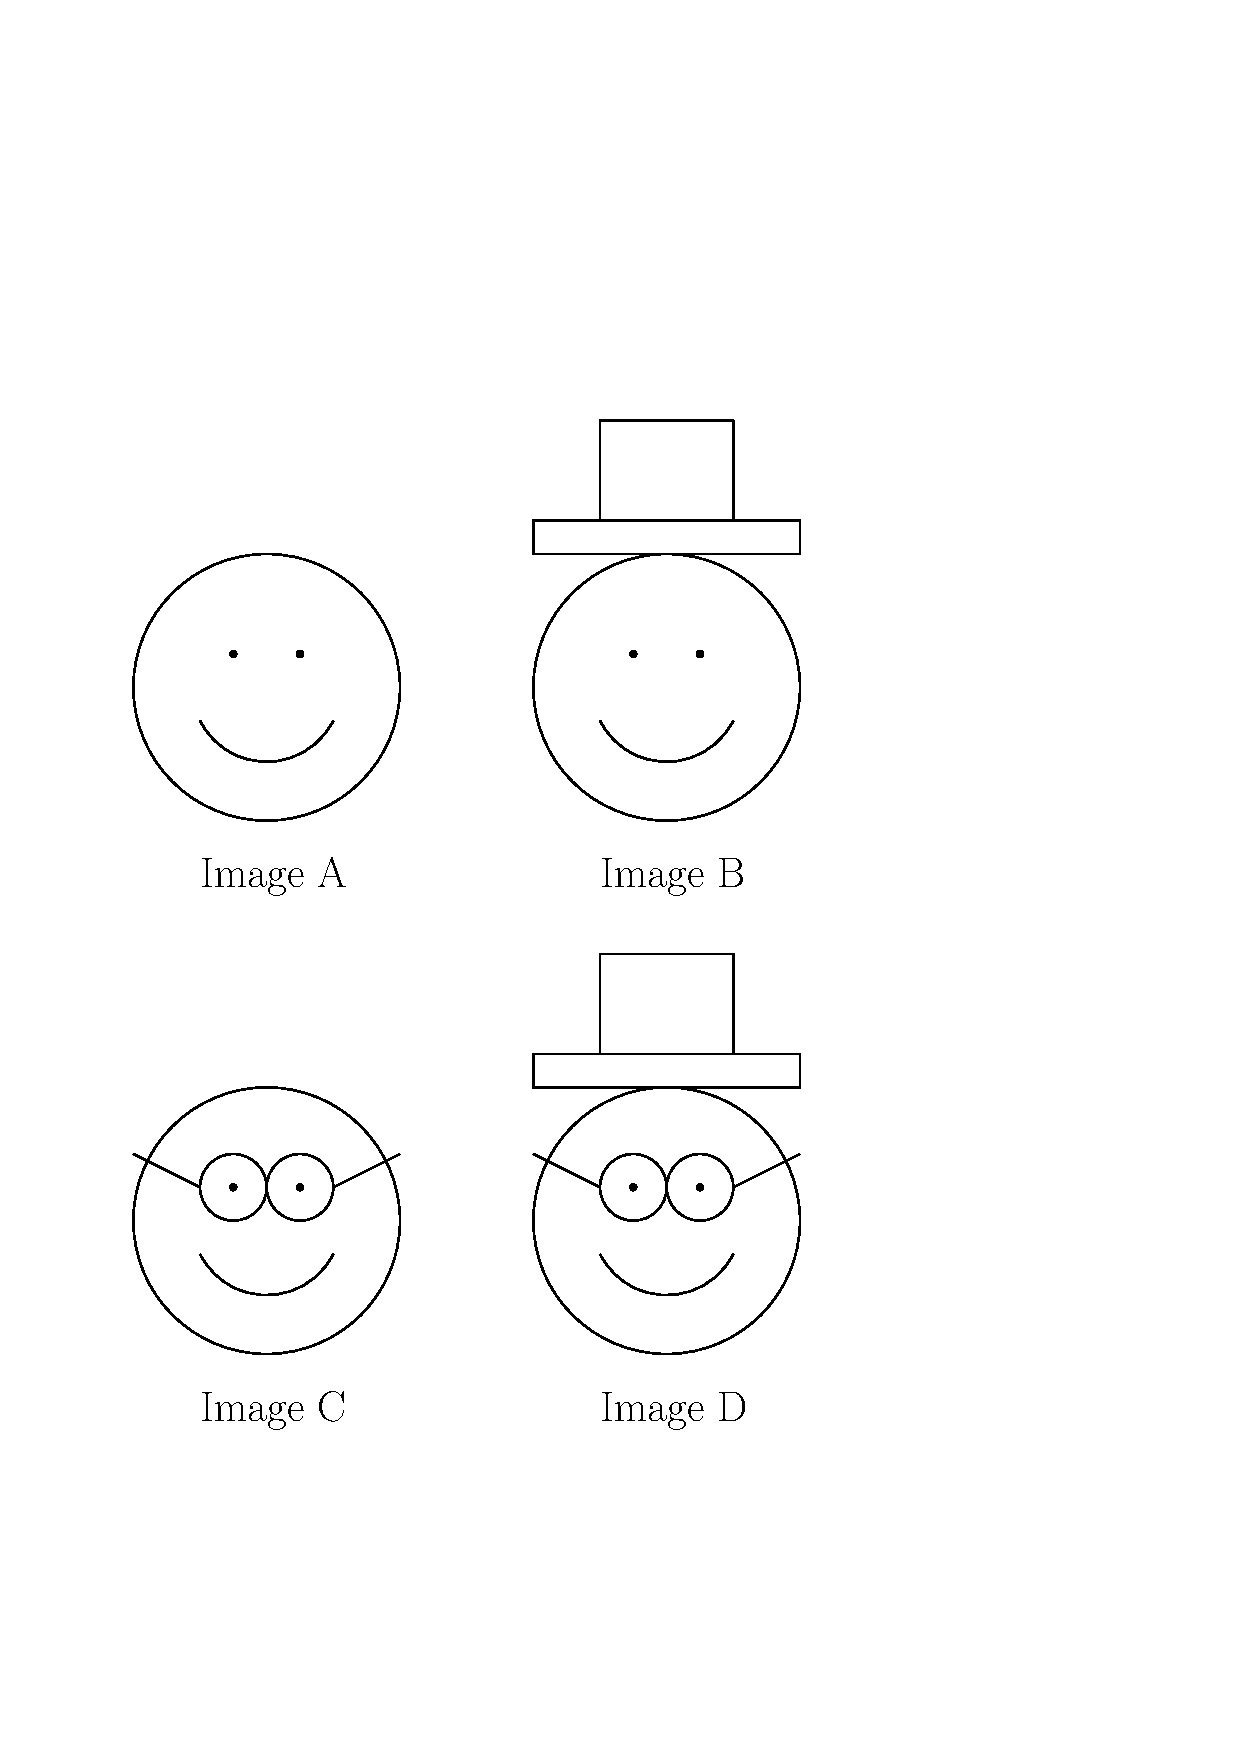
\includegraphics[width=1.5in]{images/TopHatandGlasses.pdf}
\caption{Top Hats and Glasses}\label{fig_tophatandglasses}
\end{center}
\end{figure}
%</truthTables:statement:TopHatAndGlasses:intro>  


%<*truthTables:statement:TopHatAndGlasses:imageP>  
\begin{enumerate}
\item\label{imageP} For which of the images in Figure~{\normalfont\ref{fig_tophatandglasses}} is $P$ true?
%</truthTables:statement:TopHatAndGlasses:imageP>

\Instr{  If $P$ is true then we know that I am wearing a top hat. So $P$ is true in Images B and D.}

\wbvfill
%<*truthTables:statement:TopHatAndGlasses:imageQ>  
\item\label{imageQ} For which of the images in Figure~{\normalfont\ref{fig_tophatandglasses}} is $Q$ true?
%</truthTables:statement:TopHatAndGlasses:imageQ>

\Instr{  If $Q$ is true then we know that I am wearing glasses. So $Q$ is true in images C and D.}
\wbvfill
%<*truthTables:statement:TopHatAndGlasses:imagePandQ>
\item\label{imagePandQ} For which of the images in Figure~{\normalfont\ref{fig_tophatandglasses}} is ``$P$ and $Q$'' true?
%</truthTables:statement:TopHatAndGlasses:imagePandQ>

\Instr{  If ``$P$ and $Q$'' are true, then I am wearing both a top hat and glasses. So ``$P$ and $Q$'' is only true in image D. Students may notice the intersection relationship of Questions~{\normalfont\ref{imageP}} and {\normalfont\ref{imageQ}} to answer this question. We will explore this concept further later in this chapter. We will also eventually consider ``$P$ and $Q$'' to be a single statement; such a statement is true if both $P$ and $Q$ are true, and otherwise is false.}
\wbvfill
%<*truthTables:statement:TopHatAndGlasses:imagePorQ>
\item\label{imagePorQ} For which of the images in Figure {\normalfont\ref{fig_tophatandglasses}} is ``$P$ or $Q$'' true?
%</truthTables:statement:TopHatAndGlasses:imagePorQ>

\Instr{  If ``$P$ or $Q$'' are true, then I am wearing a top hat or I am wearing glasses or I am wearing both. So ``$P$ or $Q$'' is true in images B, C, and D. Students may notice the union relationship of Questions~{\normalfont\ref{imageP}} and {\normalfont\ref{imageQ}}  to answer this question. We will explore this concept further later in this chapter.}

\wbvfill
\end{enumerate}

\newpage

%<*truthTables:statement:TopHatAndGlasses:ActivityTitle>  
\section{Making a Statement}\label{andor}
%</truthTables:statement:TopHatAndGlasses:ActivityTitle>  

\Instr{  Some students may prefer to use manipulatives to solve this problem. Cut out each of the pictures in Figure~{\normalfont\ref{fig_tophatandglasses}} to use as manipulatives.

  
\indent It is important that we be precise about what a statement\index{statement} means in this section. Each statement has the property that it is definitely true or it is definitely false. A statement may change from true to false depending on the group of objects we are considering. For example the statement ``Everyone is at least $16$ years old,'' is likely to be true if we just consider a senior high school class but is false if we consider the entire high school.}

%<*truthTables:statement:TopHatAndGlasses:ActivityAndOr>
\subsection{Activity: Exploring AND and OR Statements}
%</truthTables:statement:TopHatAndGlasses:ActivityAndOr>

%<*truthTables:statement:TopHatAndGlasses:intro4>  
\indent Consider the following statements $P$ and $Q$:
\begin{center}
\begin{tabular}{llc}
$P$: & I am wearing a top hat. & 
\includegraphics[width=.4in]{images/TopHat.pdf}\\
$Q$: & I am wearing glasses. & 
\includegraphics[width=.4in]{images/Glasses.pdf}\\
\end{tabular}
\end{center}

\begin{figure}[htb]
\begin{center}
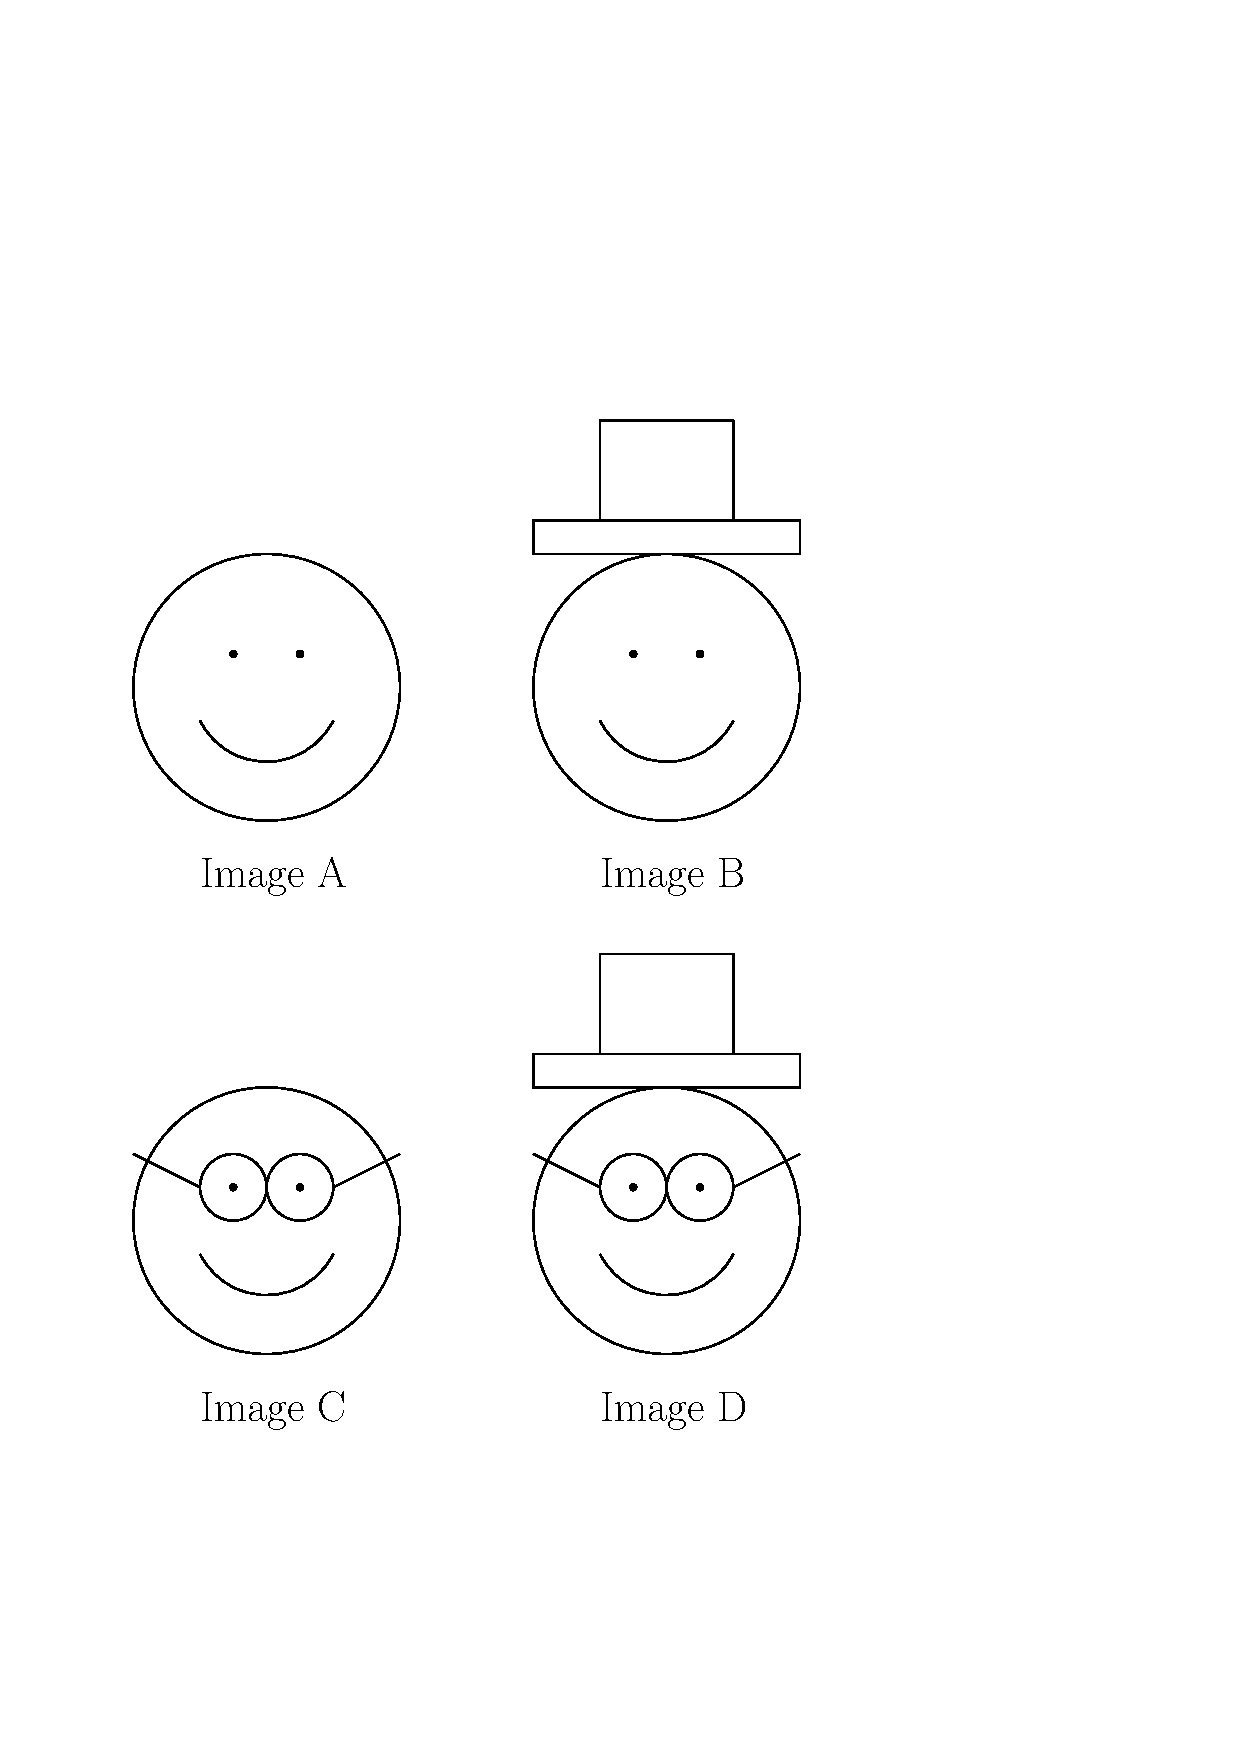
\includegraphics[width=1.5in]{images/TopHatandGlasses.pdf}
\caption{Top Hats and Glasses}\label{fig_tophatandglasses_2}
\end{center}
\end{figure}
%</truthTables:statement:TopHatAndGlasses:intro4>

\begin{enumerate}
%<*truthTables:statement:TopHatAndGlasses:bothPandQtrue>
\item What does it mean when the statement\index{statement} $P$ and the statement $Q$ are both true? Explain what it means if both $P$ and $Q$ are false?
%</truthTables:statement:TopHatAndGlasses:bothPandQtrue>

\Instr{  If $P$ and $Q$ are true, then I am wearing a top hat and glasses at the same time. If $P$ and $Q$ are both false, then I am not wearing a top hat and I am not wearing glasses. Make sure the students precisely understand these statements before moving on to the next question.}
\wbvfill
%<*truthTables:statement:TopHatAndGlasses:topHatNoGlasses>
\item If I am wearing a top hat and no glasses, would the statement\index{statement} ``$P$ and $Q$'' be true or false? Explain your answer.
%</truthTables:statement:TopHatAndGlasses:topHatNoGlasses>

\Instr{  If I am wearing a top hat, then $P$ is true. If I am not wearing glasses then $Q$ is false. So ``$P$ and $Q$'' is false; ``$P$ and $Q$'' being true means that $P$ and $Q$ are both true, so I would be wearing a top hat and glasses.}
\wbvfill

\wbnewpage

%<*truthTables:statement:TopHatAndGlasses:PorQtrue>
\item What would it mean if we knew that the statement\index{statement} ``$P$ or $Q$'' is true? Write out all the possible answers, describing the images in Figure~{\normalfont\ref{fig_tophatandglasses_2}} that make ``$P$ or $Q$'' true.
%</truthTables:statement:TopHatAndGlasses:PorQtrue>

\Instr{  The statement\index{statement} ``$P$ or $Q$'' means that I am wearing a top hat or I am wearing glasses. So there are three possibilities. Make sure the students realize that if I am wearing both a top hat then glasses and the statement ``$P$ or $Q$'' is true. }
\wbvfill

%<*truthTables:statement:TopHatAndGlasses:PorQfalse>
\item What would it mean if we knew that the statement ``$P$ or $Q$'' is false? Write out all the possible answers.
%</truthTables:statement:TopHatAndGlasses:PorQfalse>

\Instr{  If the statement\index{statement} ``$P$ or $Q$'' is false, then I am not wearing a top hat and I am not wearing glasses.}

\wbvfill
%<*truthTables:statement:TopHatAndGlasses:topHatNoGlasses2>
\item If I am wearing a top hat and no glasses, what would you say about the statement ``$P$ or $Q$''; is it true or false?
%</truthTables:statement:TopHatAndGlasses:topHatNoGlasses2>

\Instr{  If I am wearing a top hat and no glasses, then $P$ is true and $Q$ is false. So since $P$ is true, the statement\index{statement} ``$P$ or $Q$'' is true.}

\wbvfill
%<*truthTables:statement:TopHatAndGlasses:4trueFalse>
\item\label{4trueFalse} List all the different ways I can look depending on whether statement $P$ or statement $Q$ is true or false?
%</truthTables:statement:TopHatAndGlasses:4trueFalse>

\Instr{  There are $4$ possibilities: I am wearing a top hat and glasses (both $P$ and $Q$ are true), I am wearing a top hat but I am not wearing glasses ($P$ is true and $Q$ is false), I am not wearing a top hat but I am wearing glasses ($P$ is false and $Q$ is true), and I am not wearing a top hat or glasses (both $P$ and $Q$ are false).}
\wbvfill
%<*truthTables:statement:TopHatAndGlasses:end>
\end{enumerate}
%</truthTables:statement:TopHatAndGlasses:end>

\newpage

%<*truthTables:statement:tophat:intro>
\subsection{Activity: Top Hats, Overalls, and Rain boots}\label{tophat}
%</truthTables:statement:tophat:intro>

\Instr{  
Goals for this activity:
\begin{packedItem}
\item Developing situations for given compound statements; and
\item Completing Truth Tables for compound statements.
\end{packedItem}
}

%<*truthTables:statement:tophat:intro2>
\indent Let $P\wedge Q$\index{$\wedge$} be the single statement ``$P$ and $Q$'' and let $P\vee Q$\index{$\vee$} be the single statement ``$P$ or $Q$.'' Consider the statements below:
\begin{center}
\begin{tabular}{ll}
$P$: & I am wearing a top hat.\\
$Q$: & I am wearing overalls.\\
$R$: & I am wearing rain boots.\\
\end{tabular}
\end{center}

\begin{enumerate}
\setcounter{enumi}{6}
\item What do I look like if $P\wedge Q$ is true? Am I wearing the same thing if $Q\wedge P$ is true? 
%</truthTables:statement:tophat:intro2>

\Instr{  If the statement $P\wedge Q$ is true then I must be wearing both atop hat and overalls, but I may or may not be wearing rain boots. So there are two possible answers. Since $Q\wedge P$ being true means  that I am wearing overalls and a top hat, this scenario has the same two possible answers. So I may be wearing different things (i.e. ``top hat, overalls and boots'' or ``overalls, top hat, but not boots''). But since the sets of answers are the same, we say that the statement\index{statement} $P\wedge Q$ is equivalent to statement $Q\wedge P$\index{$\wedge$}.

The students may want to answer this question by ignoring $R$ completely. In such a case there is only one answer in both cases: I am wearing a top hat and overalls.}

\wbvfill
%<*truthTables:statement:tophat:PwedgeQfalse>
\item What do I look like if $P\wedge Q$ is false? Is there more than one answer? If so, list out all the possible ways I could be dressed.
%</truthTables:statement:tophat:PwedgeQfalse>

\Instr{  The students may or may not include rain boots in these answers considering that the question does not mention statement $R$. Both methods answers are correct and could be discussed as a class. If $P\wedge Q$ is false, then it is not the case that I am wearing both a top hat and overalls. Therefore, I could be wearing the overalls but not the top hat, I could be wearing a top hat but not overalls, or the only other way to be dressed would be if I can not wearing overalls and I can not wearing a top hat. So if $R$ is ignored then there are $3$ possible answers. If boots are considered by the students then each of the $3$ answers can be extended by either having me in boots or not, so then there are $6$ answers.}

\wbvfill

%<*truthTables:statement:tophat:PveeQtrue>
\item What am I wearing if $P\vee Q$\index{$\vee$} is true? Is there any difference in my outfit if $Q\vee P$ is true? List all possible outfits that make these statements\index{statement} true.
%</truthTables:statement:tophat:PveeQtrue>

\Instr{  The statement $P\vee Q$ means that I am wearing a top hat or I am wearing overalls, so I can be wearing only the top hat and not the overalls, I can be wearing overalls and not the top hat, or I can be wearing both the top hat and the overalls. All of these answers can be written with or without rain boots, giving a total of $3$ possible solutions if the students do not include the rain boots in the problem  and $6$ possible solutions otherwise. 

As before, there is no difference between the set of answers that make the statements $P\vee Q$ and $Q\vee P$ true, so they are equivalent.}

\wbvfill
%<*truthTables:statement:tophat:logicTable>
\item\label{logicTable} Fill in the table below. Each cell in the table should contain either ``True'' or ``False.'' First write in all the possible truth values for the pair of statements\index{statement} $P$ and $Q$ in the first two columns (see Question~{\normalfont\ref{4trueFalse}} for some help). Then in the third and fourth columns describe how $P\wedge Q$\index{$\wedge$} and $P\vee Q$\index{$\vee$} will be affected by your choice of $P$ and $Q$ in the corresponding row. This table is called a truth table\index{truth table}.
\begin{center}
\begin{tabular}{|c|c||c|c|}
\hline
$P$ & $Q$ & $P\wedge Q$ & $P\vee Q$ \\
\hline
\hline
\hspace{.75in} & \hspace{.75in} & \hspace{.75in} & \hspace{.75in} \\
\hline
 &  & & \\
\hline
 & & & \\
\hline
 & & & \\
\hline
\end{tabular}
\end{center}
%</truthTables:statement:tophat:logicTable>

\Instr{ 
The order in which the rows are listed in the following table is not important.
\begin{center}
\begin{tabular}{|c|c||c|c|}
\hline
$P$ & $Q$ & $P\wedge Q$ & $P\vee Q$ \\
\hline
\hline
True & True & True & True \\
\hline
True & False & False & True \\
\hline
False & True & False & True \\
\hline
False & False & False & False \\
\hline
\end{tabular}
\end{center}
}

\wbnewpage

%<*truthTables:statement:tophat:PandQandR2>
\item\label{PandQandR2} What do I look like if $P\wedge Q\wedge R$ is true? 
%</truthTables:statement:tophat:PandQandR2>

\Instr{  If $P\wedge Q\wedge R$ is true then I am wearing a top hat and overalls and rain boots. There is only one possible answer.}
\wbvfill
%<*truthTables:statement:tophat:order?>
\item Does my outfit change if we reorder $P$, $Q$, and $R$ in Question~{\normalfont\ref{PandQandR2}}? Explain your answer.
%</truthTables:statement:tophat:order?>

\Instr{  No matter the order of the articles that I am wearing, the statements\index{statement} $P\wedge Q\wedge R$\index{$\wedge$}, $P\wedge R\wedge Q$, $R \wedge P \wedge Q$, $R\wedge Q\wedge P$, $Q\wedge P \wedge R$, and $Q\wedge R\wedge P$ are all equivalent. The reason for this is because for $P\wedge Q\wedge R$ to be true, the statements $P$, $Q$, and $R$ must all be true. If any one of these statements are false then $P\wedge Q \wedge R$ is false.}
\wbvfill
%<*truthTables:statement:tophat:describePorQandR>
\item\label{describePorQandR} Describe my clothing if $(P\vee Q) \wedge R$ is true. List out all the possible clothing options. \Hint{ There are three.}
%</truthTables:statement:tophat:describePorQandR>

\Instr{  The statement\index{statement} $(P\vee Q)\wedge R$\index{$\vee$} means that I am wearing a top hat and rain boots, I am wearing overalls and rain boots, or I am wearing a top hat, overalls, and rain boots. If this statement is true, then notice that $R$ must be true and $P\vee Q$ must be true. Thus I must be wearing rain boots, and I must be wearing overalls or a top hat.
}
\wbvfill
%<*truthTables:statement:tophat:describePorQandR2>
\item\label{describePorQandR2} Describe my clothing if $P\vee (Q\wedge R)$ is true. List out all the possible clothing options. \Hint{ There are five.}
%</truthTables:statement:tophat:describePorQandR2>

\Instr{  The statement\index{statement} $P\vee (Q\wedge R)$\index{$\vee$}\index{$\wedge$} says I am wearing a top hat, I am wearing overalls and rain boots, or I am wearing a top hat, overalls, and rain boots.}
\wbvfill
%<*truthTables:statement:tophat:describePorQandR3>

\wbnewpage
\item\label{describePorQandR3} Fill in the table below. Each cell in the table should contain either ``True'' or ``False.'' As in Question~{\normalfont\ref{logicTable}} first fill in the first three columns so that no two rows have exactly the same three truth values for $P$, $Q$ and $R$. The your choice of $P$, $Q$, and $R$ in each row will determine the truth value in the next three columns. \Hint{ see questions~{\normalfont\ref{describePorQandR}} and~{\normalfont\ref{describePorQandR2}}.}
\begin{center}
\begin{tabular}{|c|c|c||c|c|}
\hline
$P$ & $Q$ & $R$ & $(P\vee Q) \wedge R$ & $P\vee (Q \wedge R)$ \\
\hline
\hline
\hspace{.75in} & \hspace{.75in} & \hspace{.75in} & \hspace{.75in} & \hspace{.75in} \\
\hline
 & & & & \\
\hline
 & & & & \\
\hline
 & & & & \\
\hline
 & & & & \\
\hline
 & & & & \\
\hline
 & & & & \\
\hline
 & & & & \\
\hline
\end{tabular}
\end{center}
%</truthTables:statement:tophat:describePorQandR3>

\Instr{  
The order of the rows in the following table is not important.
\begin{center}
\begin{tabular}{|c|c|c||c|c|}
\hline
$P$ & $Q$ & $R$ & $(P\vee Q) \wedge R$ & $P\vee (Q \wedge R)$ \\
\hline
\hline
True & True & True & True & True \\
\hline
True & True & False & False & True \\
\hline
True & False & True & True & True \\
\hline
True & False & False & False & True \\
\hline
False & True & True  & True & True \\
\hline
False & True & False & False & False \\
\hline
False & False & True & False & False \\
\hline
False & False & False & False & False \\
\hline
\end{tabular}
\end{center}
}
%<*truthTables:statement:tophat:describePorQandR4>
\item Using the truth table\index{truth table} in Question~{\normalfont\ref{describePorQandR3}} determine if the statement\index{statement} $P\vee (Q\wedge R)$\index{$\vee$}\index{$\wedge$} the same as the statement $(P\vee Q)\wedge R$. Explain yourself thoroughly.
%</truthTables:statement:tophat:describePorQandR4>

\Instr{  Just by reading over the meanings of these statements it is clear that $(P\vee Q)\wedge R$ is not the same as $P\vee (Q\wedge R)$. The truth table in Question~{\normalfont\ref{describePorQandR3}} also tells us the same conclusions that when $P$ is true and $R$ is false, the two statements are not equivalent regardless of the truth value for $Q$.}

\wbvfill
%<*truthTables:statement:tophat:PandQandR>
\item\label{PandQandR} Suppose I am wearing a top hat and rain boots, and I am not wearing overalls. Is the statement\index{statement} $(P\wedge Q) \wedge R$\index{$\wedge$}\index{$\vee$} true or false? Is the statement $(P\wedge R) \vee Q$ true or false?
%</truthTables:statement:tophat:PandQandR>

\Instr{  According to the question given, $P$ is true, $Q$ is false, and $R$ is true. Since $P\wedge Q$ is false, $(P\wedge Q)\wedge R$ is false. Similarly, since $P\wedge R$ is true, $(P\wedge R) \vee Q$ is true.}

\wbvfill
\end{enumerate}

\newpage

\subsection{Exit Slip}

%<*truthTables:statement:tophat:logicTable2>
 Fill in the table below. Each cell in the table should contain either ``True'' or ``False.'' As in Question~{\normalfont\ref{logicTable}}, begin by completing the first three columns.
\begin{center}
\begin{tabular}{|c|c|c||c|c|c|}
\hline
$P$ & $Q$ & $R$ & $(P\wedge Q) \wedge R$ & $(P\vee Q) \vee R$ & $P\vee (Q \wedge R)$ \\
\hline
\hline
\hspace{.75in} & \hspace{.75in} & \hspace{.75in} & \hspace{.75in} & \hspace{.75in} & \hspace{.75in} \\
\hline
 & & & & & \\
\hline
 & & & & & \\
\hline
 & & & & & \\
\hline
 & & & & & \\
\hline
 & & & & & \\
\hline
 & & & & & \\
\hline
 & & & & & \\
\hline
\end{tabular}
\end{center}
%</truthTables:statement:tophat:logicTable2>

\Instr{  
\begin{center}
\begin{tabular}{|c|c|c||c|c|c|}
\hline
$P$ & $Q$ & $R$ & $(P\wedge Q) \wedge R$ & $(P\vee Q) \vee R$ & $P\vee (Q \wedge R)$ \\
\hline
\hline
True & True & True & True & True & True \\
\hline
True & True & False & False & True & True \\
\hline
True & False & True & False & True & True \\
\hline
True & False & False & False & True & True \\
\hline
False & True & True & False & True & True \\
\hline
False & True & False & False & True & False \\
\hline
False & False & True & False & True & False \\
\hline
False & False & False & False & False & False \\
\hline
\end{tabular}
\end{center}
}
%<*truthTables:statement:tophat:end>
%</truthTables:statement:tophat:end>

%<*truthTables:statement:tophat:exit>


%</truthTables:statement:tophat:exit>
\newpage

%<*truthTables:statement:negation:intro>
\subsection{Activity: Negation}\label{negation}
%</truthTables:statement:negation:intro>

\Instr{  
Goals for this activity:
\begin{packedItem}
\item Working with negations withing compound statements; 
\item Determining truth values of compound statements containing negations; 
\item Completing Truth Tables for compounstatements containing negations; and
\item Determining weather two statements are equivalent.
\end{packedItem}
}

%<*truthTables:statement:negation:intro2>
\indent Let $\neg P$ represent the statement\index{statement} ``$P$ is false''. ($\neg P$\index{$\neg$} is called the negation of $P$.) Again we will consider the statements below.
\begin{center}
\begin{tabular}{ll}
$P$: & I am wearing a top hat.\\
$Q$: & I am wearing overalls.\\
$R$: & I am wearing rain boots.\\
\end{tabular}
\end{center}

\begin{enumerate}
\setcounter{enumi}{26}
\item\label{negPtrue} If $\neg P$ is true, is anything on my head? 
%</truthTables:statement:negation:intro2>

\Instr{  When $\neg P$ is true, ``$P$ is false'' is true, so I am not wearing a top hat. So there maybe something on my head, but it is not a top hat!}

\wbvfill
%<*truthTables:statement:negation:negPtrue>
\item If $\neg P$ is false, is anything on my head?
%</truthTables:statement:negation:negPtrue>

\Instr{  When $\neg P$ is false, ``$P$ is false'' is false, so $P$ is true. Therefore there is something on my head when $\neg P$ is false, namely a top hat.}
\wbvfill
%<*truthTables:statement:negation:negPfalse>
\item Fill in the truth table\index{truth table} below. Each cell in the table should contain either ``True'' or ``False.'' As in Question~{\normalfont\ref{logicTable}} begin by completing the first column.
\begin{center}
\begin{tabular}{|c||c|}
\hline
$P$ & $\neg P$ \\
\hline
\hline
\hspace{.75in} & \hspace{.75in} \\
\hline
& \\
\hline
\end{tabular}
\end{center}
%</truthTables:statement:negation:negPfalse>

\Instr{  
\begin{center}
\begin{tabular}{|c||c|}
\hline
$P$ & $\neg P$ \\
\hline
\hline
True & False \\
\hline
False & True \\
\hline
\end{tabular}
\end{center}
}

%<*truthTables:statement:negation:PwedgeRfalse>
\item Suppose you know the statement $P\wedge R$\index{$\wedge$} is false. Describe what I'm wearing. Is there a statement that says the same thing when it is true?
%</truthTables:statement:negation:PwedgeRfalse>

\Instr{  If $P\wedge R$ is false then it is not the case that I am wearing both a top hat and rain boots. Therefore I am either ``not wearing a top hat'' or ``I am not wearing rain boots.'' The easiest way to find a corresponding true statement is to simply apply the $\neg$ function and use $\neg (P\wedge R)$. But the verbal description of what I'm wearing leads to another solution: $\neg P \vee \neg Q$\index{$\neg$}\index{$\vee$}. Encourage the students to find both answers.}

\wbvfill

\newpage

%<*truthTables:statement:negation:QveeRfalse>
\iffalse
\item Suppose you know the statement $Q\vee R$ is false. Describe what I'm wearing. Is there a statement\index{statement} that says the same thing when it is true?
%</truthTables:statement:negation:QveeRfalse>

\Instr{  If $Q\vee R$ is false then it is not the case that either I am wearing overalls or I am wearing rain boots. So I cannot be wearing either. Therefore I am not wearing overalls and I am not wearing rain boots. So both the statement\index{statement} $\neg Q \wedge \neg R$\index{$\neg$}\index{$\wedge$} is true. What I am wearing is also described by $\neg(Q\wedge R)$, as can be seen by applying the definition of $\neg$. So both are good answers.}

%<*truthTables:statement:negation:PwedgenegQfalse>
\item Suppose you know that statement $P\wedge \neg Q$ is false. Describe what I'm wearing. Is there a statement that says the same thing when it is true?
%</truthTables:statement:negation:PwedgenegQfalse>

\Instr{  If $P\wedge \neg Q$ is false then it is not the case that I am both wearing a top hat and not wearing overalls. Therefore either I am not wearing a top hat or I am wearing overalls. So the statement\index{statement} $\neg P\vee Q$\index{$\neg$}\index{$\vee$}\index{$\wedge$} is true. Also, $\neg(P\wedge \neg Q)$ is true by the definition of $\neg$. So both are good answers.}
\fi
%<*truthTables:statement:negation:logicTable2.5>
\item\label{logicTable2.5} Fill in the truth table\index{truth table} below so that each cell contains either ``True'' or ``False.'' As in Question~{\normalfont\ref{logicTable}}, begin by completing the first two columns so that all ways truth values can be assigned to $P$ and $Q$ are represented in the four rows.
\begin{center}
\begin{tabular}{|c|c||c|c|c|c|}
\hline
$P$ & $Q$ & $\neg P$ & $\neg Q$ & $\neg(P\wedge Q)$ & $\neg P\vee \neg Q$ \\
\hline
\hline
\hspace{.5in} & \hspace{.5in} & \hspace{.5in} & \hspace{.5in} & \hspace{.75in} & \hspace{.75in} \\
\hline
&&&&& \\
\hline
&&&&& \\
\hline
&&&&& \\
\hline
\end{tabular}
\end{center}
%</truthTables:statement:negation:logicTable2.5>

\Instr{ 
\begin{center}
\begin{tabular}{|c|c||c|c|c|c|}
\hline
$P$ & $Q$ & $\neg P$ & $\neg Q$ & $\neg (P\wedge Q)$ & $\neg P\vee \neg Q$ \\
\hline
\hline
True & True & False & False & False & False  \\
\hline
True & False & False & True & True & True  \\
\hline
False & True & True & False & True & True \\
\hline
False & False & True & True & True & True \\
\hline
\end{tabular}
\end{center}
}

%<*truthTables:statement:negation:sameStatement?>
\item Using the truth table\index{truth table} in Question~{\normalfont\ref{logicTable2.5}} determine if the statement $\neg(P\wedge R)$ is the same as the statement\index{statement}\index{$\wedge$}\index{$\vee$}\index{$\neg$} $\neg P \vee \neg R$. Explain yourself thoroughly.
%</truthTables:statement:negation:sameStatement?>

\Instr{  Based on the truth table they are the same. Also, by reasoning out what each of the statements is saying, it is clear that the two statements are identical.}

\iffalse
%<*truthTables:statement:negation:logicTable3>
\item\label{logicTable3} Fill in the table below so that each cell contains either ``True'' or ``False.'' As in Question~{\normalfont\ref{logicTable}}, begin by completing the first two columns.
\begin{center}
\begin{tabular}{|c|c||c|c|c|c|c|}
\hline
$P$ & $Q$ & $\neg P$ & $\neg Q$ & $\neg P\wedge Q$ & $P\vee \neg Q$ & $\neg P\vee \neg Q$ \\
\hline
\hline
\hspace{.5in} & \hspace{.5in} & \hspace{.5in} & \hspace{.5in} & \hspace{.75in} & \hspace{.75in} & \hspace{.75in} \\
\hline
&&&&&& \\
\hline
&&&&&& \\
\hline
&&&&&& \\
\hline
\end{tabular}
\end{center}
%</truthTables:statement:negation:logicTable3>

\Instr{  
\begin{center}
\begin{tabular}{|c|c||c|c|c|c|c|}
\hline
$P$ & $Q$ & $\neg P$ & $\neg Q$ & $\neg P\wedge Q$ & $\neg P\vee \neg Q$ & $P\vee \neg Q$ \\
\hline
\hline
True & True & False & False & False & False & True \\
\hline
True & False & False & True & False & True & True \\
\hline
False & True & True & False & True & True & False \\
\hline
False & False & True & True & False & True & True \\
\hline
\end{tabular}
\end{center}
}
\fi

\wbvfill
%<*truthTables:statement:negation:logicTable4>
\item\label{logicTable4} Fill in the table below so that each cell contains either ``True'' and ``False.'' As in Question~{\normalfont\ref{logicTable}}, begin by completing the first three columns.
\begin{center}
\begin{tabular}{|c|c|c||c|c|c|}
\hline
$P$ & $Q$ & $R$ & $(P\wedge Q) \wedge \neg R$ & $(\neg P \vee \neg Q) \vee R$ & $(P\vee \neg Q) \wedge \neg R$ \\
\hline
\hline
\hspace{.44in} & \hspace{.44in} & \hspace{.44in} &&& \\
\hline
&&&&& \\
\hline
&&&&& \\
\hline
&&&&& \\
\hline
&&&&& \\
\hline
&&&&& \\
\hline
&&&&& \\
\hline
&&&&& \\
\hline
\end{tabular}
\end{center}
%</truthTables:statement:negation:logicTable4>

\Instr{  
\begin{center}
\begin{tabular}{|c|c|c||c|c|c|}
\hline
$P$ & $Q$ & $R$ & $(P\wedge Q) \wedge \neg R$ & $(\neg P \vee \neg Q) \vee R$ & $(P\vee \neg Q) \wedge \neg R$ \\
\hline
\hline
True & True & True & False & True & False \\
\hline
True & True & False & True & False & True \\
\hline
True & False & True & False & True & False \\
\hline
True & False & False & False & True & True \\
\hline
False & True & True & False & True & False \\
\hline
False & True & False & False & True & False \\
\hline
False & False & True & False & True & False \\
\hline
False & False & False & False & True & True \\
\hline
\end{tabular}
\end{center}
}


%<*truthTables:statement:negation:end>
\end{enumerate}
%</truthTables:statement:negation:end>

\newpage

\subsection{Activity: The Implications\index{implication} of Your Actions}\label{implications}
%</truthTables:implications:title>

\Instr{  
Goals for this activity:
\begin{packedItem}
\item Making truth tables for implication statements; 
\item Writing symbolic statements which represent a given written statements; and
\item Creating equivalent statements using implication conjunctions.
\end{packedItem}
}

%<*truthTables:implications:intro>
The last activity introduced the basic form of an argument used by mathematicians. They assume that something is true and then see if that means whether you know other things are true. This step is called an \textbf{implication}\index{implication}. We say that ``$P$ implies $Q$'', and write $P\Rightarrow Q$, if whenever $P$ is true $Q$ is also true. So the only way that the statement\index{statement} $P\Rightarrow Q$\index{$\wedge$} can be false is when $P$ is true and $Q$ is false. 

\begin{enumerate}
\item Consider the statement ``If it's Monday, my day will suck.'' This is an implication where $P = $ ``today is Monday'' and $Q = $ ``I will have a sucky day today.''  Discuss with your group members:  What are the 4 possible options for T/F for $P$ and $Q$.  In which of those scenarios is the person who claims ``If it's Monday, my day will suck'' saying something true?  In which scenario are they wrong?

\wbvfill

\item\label{implyTable} Fill in the following table so that each cell contains either ``True'' or ``False.'' First write in all the possible truth values for the pair of statements $P$ and $Q$ in the first two columns. Then in the third column indicate how $P\Rightarrow Q$ will be affected by your choice of $P$ and $Q$ in the corresponding row. 

\begin{center}
\begin{tabular}{|c|c||c|}
\hline
$P$ & $Q$ & $P\Rightarrow Q$ \\
\hline
\hline
\hspace{.4in} & \hspace{.4in} & \hspace{.4in}  \\
\hline
&& \\
\hline
&& \\
\hline
&& \\
\hline
\end{tabular}
\end{center}
%</truthTables:implications:intro>

\Instr{  The students may not know what to fill in for $P\Rightarrow Q$\index{$\Rightarrow$} when $P$ is false. Point them to the definition where it says there is only one way to make $P\Rightarrow Q$ false.
\begin{center}
\begin{tabular}{|c|c||c|}
\hline
$P$ & $Q$ & $P\Rightarrow Q$ \\
\hline
\hline
True & True & True \\
\hline
True & False & False \\
\hline
False & True & True \\
\hline
False & False & True \\
\hline
\end{tabular}
\end{center}
}

%<*truthTables:implications:PimpliesQ>
\item Notice that $P\Rightarrow Q$ is always true whenever $P$ is false. Why do you think that is the case?
%</truthTables:implications:PimpliesQ>

\Instr{  $P\Rightarrow Q$ only tries to assert something about $Q$ when $P$ is itself true. If $P$ is false, then $P\Rightarrow Q$ is not trying to assert anything, so it cannot be false.
}

\wbvfill

\wbnewpage

%<*truthTables:implications:tuesdayRaining>
\item Suppose the statement\index{statement} ``If it is Tuesday then it must be raining all day'' is true. What do you know if:
\begin{enumerate}
\item it is not raining outside.
\wbvfill

\item it is Tuesday today.
\wbvfill
\item it is Wednesday today.
\wbvfill
\end{enumerate}
%</truthTables:implications:tuesdayRaining>

\Instr{  \begin{enumerate}
\item It cannot be Tuesday (because on Tuesday it is raining).
\item It is raining all day today.
\item We do not know anything about the weather. It is worth asking the students to assign a letter to the two statements in the implication\index{implication}, say
\begin{center}
\begin{tabular}{ll}
$T$: & It is Tuesday. \\
$R$: & It is raining all day. \\
\end{tabular}
\end{center}
Then ask the students

\begin{minipage}[H]{5.75in}
\tt \em
\begin{center}
{``What are we told is true?''}
\end{center}
\end{minipage}

We know $T\Rightarrow R$ is true. Then ask

\begin{minipage}[H]{5.75in}
\tt \em
\begin{center}
{``What does each of (a), (b), and (c) tell us about the truth value of $T$ and $R$?''}
\end{center}
\end{minipage}

and then

\begin{minipage}[H]{5.75in}
\tt \em
\begin{center}
{``How does this help you answer the question?''}
\end{center}
\end{minipage}

To this you can answer
\begin{enumerate}
\item[(a)] $R$ is false. But $T\Rightarrow R$ is true. So from the table in Question~{\normalfont\ref{implyTable}} we know that $T$ must be false.
\item[(b)] $T$ is true. But $T\Rightarrow R$ is also true. So from the table in Question~{\normalfont\ref{implyTable}} $R$ must be true.
\item[(c)] $T$ is false. So from the table in Question~{\normalfont\ref{implyTable}}, $R$ could be true or false.
\end{enumerate}
\end{enumerate}
}

%<*truthTables:implications:endRainUmbrella>
\end{enumerate}		

\newpage
Consider the statements below for Questions~{\normalfont\ref{P->Q}}--{\normalfont\ref{P->RandS}}.
\begin{center}
\begin{tabular}{ll}
$P$: & It is raining today. \\
$Q$: & I bring an umbrella with me. \\
$R$: & I play basketball during recess. \\
$S$: & I took a test in English class. \\
\end{tabular}
\end{center}

\begin{enumerate}
\setcounter{enumi}{3}
\item\label{P->Q} Write the statement

\begin{minipage}[H]{5.75in}
\tt \em 
\begin{center}
{``If it is raining today then I will bring an umbrella with me.''}
\end{center}
\end{minipage}

\noindent using the symbolic statements $P$, $Q$, $R$, and $S$. Explain why you know your answer is correct.
%</truthTables:implications:endRainUmbrella>

\Instr{  This is to make sure the students have a understanding of symbolic statements of implications\index{implication}. The answer should be $P \Rightarrow Q$\index{$\Rightarrow$}. }

\wbvfill

\iffalse
%<*truthTables:implications:P->P>
\item\label{P->P} Write the statement\index{statement}

\begin{minipage}[H]{5.75in}
\tt \em
\begin{center}
{``If it is raining today then it is raining today.'' }
\end{center}
\end{minipage}

\noindent using the symbolic statements $P$, $Q$, $R$, and $S$. Explain why you know your answer is correct.
%</truthTables:implications:P->P>

\Instr{  The answer is $P \Rightarrow P$. This is a good time to have students really think about what they are writing. This statement seems a bit trivial intact it is always true. We will explore other statements that are always true that do not seem as trivial later.}

\fi
%<*truthTables:implications:P->RandS>
\item\label{P->RandS} Write the statement\index{statement}

\begin{minipage}[H]{5.75in}
\tt \em
\begin{center}
{``If it is raining today then I will play basketball and take a test in English class.''}
\end{center}
\end{minipage}

\noindent using the symbolic statements $P$, $Q$, $R$, and $S$. Explain why you know your answer is correct.
%</truthTables:implications:P->RandS>

\Instr{   This is a time when we must discuss how the order and wording of a sentence can affect the symbolic statements. This statement seems to have two possible answers if one does not technically define what is meant by the statement. The confusion is derived when we we consider the ``and'' portion of the statement.

 We must decide weather the ``and'' statement\index{statement} is applied inside the implication or if the implication\index{implication} is applied inside the ``and'' statement. Students may write the statement as $(P\Rightarrow R) \wedge S$\index{$\wedge$}, but there is a subtlety in the fact that there is only one ``I will'' in the statement therefore providing a clue that the statement is intended to be $P \Rightarrow (R \wedge S)$ because the statement infers that if it is raining then we will do both of the following (play basketball and take the test.
 
 This might be a good time to discuss ordering of sentences. If we wanted to mean $(P\Rightarrow R) \wedge S$ it is possible to place another ``I will'' after the ``and'' in the above sentence but better than that we can reorder the sentence. This is possible since the ``and'' conjunction is associative. So we would write ``I will take a test in English class  and If it is raining today then I will play basketball.'' which is symbolically written as $S \wedge (P\Rightarrow R)$\index{$\Rightarrow$} and obviously equivalent to  $(P\Rightarrow R) \wedge S$}

\wbvfill
\iffalse
%<*truthTables:implications:RorQ->P>
\item \label{RorQ->P} Write the statement\\
\begin{minipage}[H]{5.75in}
\tt \em 
\begin{center}
{``If I play basketball today or I brought my umbrella with me then it is raining today.''}
\end{center}
\end{minipage}\\
using the symbolic statements\index{statement} $P$, $Q$, $R$, and $S$. Explain why you know your answer is correct.
%</truthTables:implications:RorQ->P>

\Instr{  Again we have combined previously mentioned conjunctions with an implication\index{implication}, but here there should be no issue to which statement is inside the other, however if we are not careful with our use of parenthesis we could write a symbolic statement which is not indicative of the statement which is written. The students should be written as $(R \vee Q) \Rightarrow P$\index{$\vee$}\index{$\Rightarrow$}. But it should be noted that if we leave the parenthesis off we have written a symbolic statement where the implication\index{implication} is inside the ``or'' statement, which is not an accurate representation of the statement given.}

\fi
%<*truthTables:implications:implicationsTable>
\item\label{implicationsTable} Fill in Table~{\normalfont\ref{implicationsTable1}} so that each cell contains either ``True'' or ``False.'' First write in all the possible truth values for the pair of statements $P$ and $Q$ in the first two columns. Then in the remaining columns indicate how the other statements will be affected by your choice of $P$ and $Q$ in the corresponding row.

\index{$\neg$}\index{$\Rightarrow$}
\begin{table}[htb]
\begin{center}
\begin{tabular}{|c|c||c|c|c|c|c|c|}
\hline
\strut $P$ & $Q$ & $\neg P$ & $\neg Q$ & $P\Rightarrow Q$ & $Q\Rightarrow P$ & $\neg P \Rightarrow \neg Q$ & $\neg Q \Rightarrow \neg P$\\
\hline
\hline
\strut \hspace{.4in} & \hspace{.4in} & \hspace{.4in} & \hspace{.4in} & \hspace{.7in} & \hspace{.7in} & \hspace{.7in} & \hspace{.7in}  \\
\hline
\strut&&&&&&& \\
\hline
\strut&&&&&&& \\
\hline
\strut&&&&&&& \\
\hline
\end{tabular}
\caption{Table of logical statements\index{statement} using the $\Rightarrow$ symbol}\label{implicationsTable1}
\end{center}
\end{table}
%</truthTables:implications:implicationsTable>

\wbnewpage

\Instr{ 
\begin{center}
\begin{tabular}{|c|c||c|c|c|c|c|c|}
\hline
$P$ & $Q$ & $\neg P$ & $\neg Q$ & $P\Rightarrow Q$ & $Q\Rightarrow P$ & $\neg P \Rightarrow \neg Q$ & $\neg Q \Rightarrow \neg P$\\
\hline
\hline
True&True&False&False&True&True&True&True \\
\hline
True&False&False&True&False&True&True&False \\
\hline
False&True&True&False&True&False&False&True \\
\hline
False&False&True&True&True&True&True&True \\
\hline
\end{tabular}
\end{center}
}

%<*truthTables:implications:P->QTrue>
\item If $P\Rightarrow Q$ is true, does that mean that $Q\Rightarrow P$ is true. Give a justification for your answer.
%</truthTables:implications:P->QTrue>

\Instr{  No. In the third row we see that $P \Rightarrow Q$ is true, but $Q \Rightarrow P$ is false. }

\wbvfill

%<*truthTables:implications:symbolicStatements>
\item Which symbolic statements\index{statement} in the Table~{\normalfont\ref{implicationsTable1}} are equivalent?
%</truthTables:implications:symbolicStatements>

\Instr{  The students should notice that there are two pairs of identical rows. the rows of $P \Rightarrow Q$ and $\neg Q \Rightarrow \neg P$ produce the same outcome thus proving to be equivalent statements. Similarly  statements $Q\Rightarrow P$ and $\neg P \Rightarrow \neg Q$ are equivalent.}

\wbvfill
%<*truthTables:implications:end>
\end{enumerate}
%</truthTables:implications:end>

\newpage
%<*truthTables:Minesweeper:Title>
\section{Logic in Games}\label{Minesweeper}
%</truthTables:Minesweeper:Title>

\subsection{Entrance Activity: Statements in Minesweeper}

The game of Minesweeper is a popular game that requires players to use logic to solve the puzzle. The game begins with a board of squares, some of which contain hidden mines. Game play can be summarized in one sentence: \textbf{the number on a block shows the number of mines adjacent to it and you have to flag all the mines}. In more detail:
\begin{itemize}
	\item Start by clicking any random place since it is your first move. You do not have any clues to the locations of the mines yet!
    \item When you identify a square hiding a mine, flag it by right-clicking. This will place a flag on that spot.
    \item When you identify a square that is not hiding a mine, clear it by clicking it. This will reveal the number of mines in the adjacent squares, or more if there are no adjacent mines.
    \item If you accidentally clear a mine you lose. 
    \item If you flag all the mines and clear all other locations, you win!
\end{itemize}

\noindent Before reading any further go to \href{https://freeminesweeper.org/}{https://freeminesweeper.org/} and play a few games! If it is your first time playing, you might want to select Beginner from the Game menu.

Here is a sample of the type of question you will be asked and how you are expected to answer. Shown is a game in progress where the player has indicated the locations of 4 mines (marked by the 4 flags). The 6 above the game board and on the left indicates there are 6 remaining mines. In this example, we have labelled one location with the letter ``A'' to indicate a space we would like to discuss. You will not see letters on the squares while playing the game online.

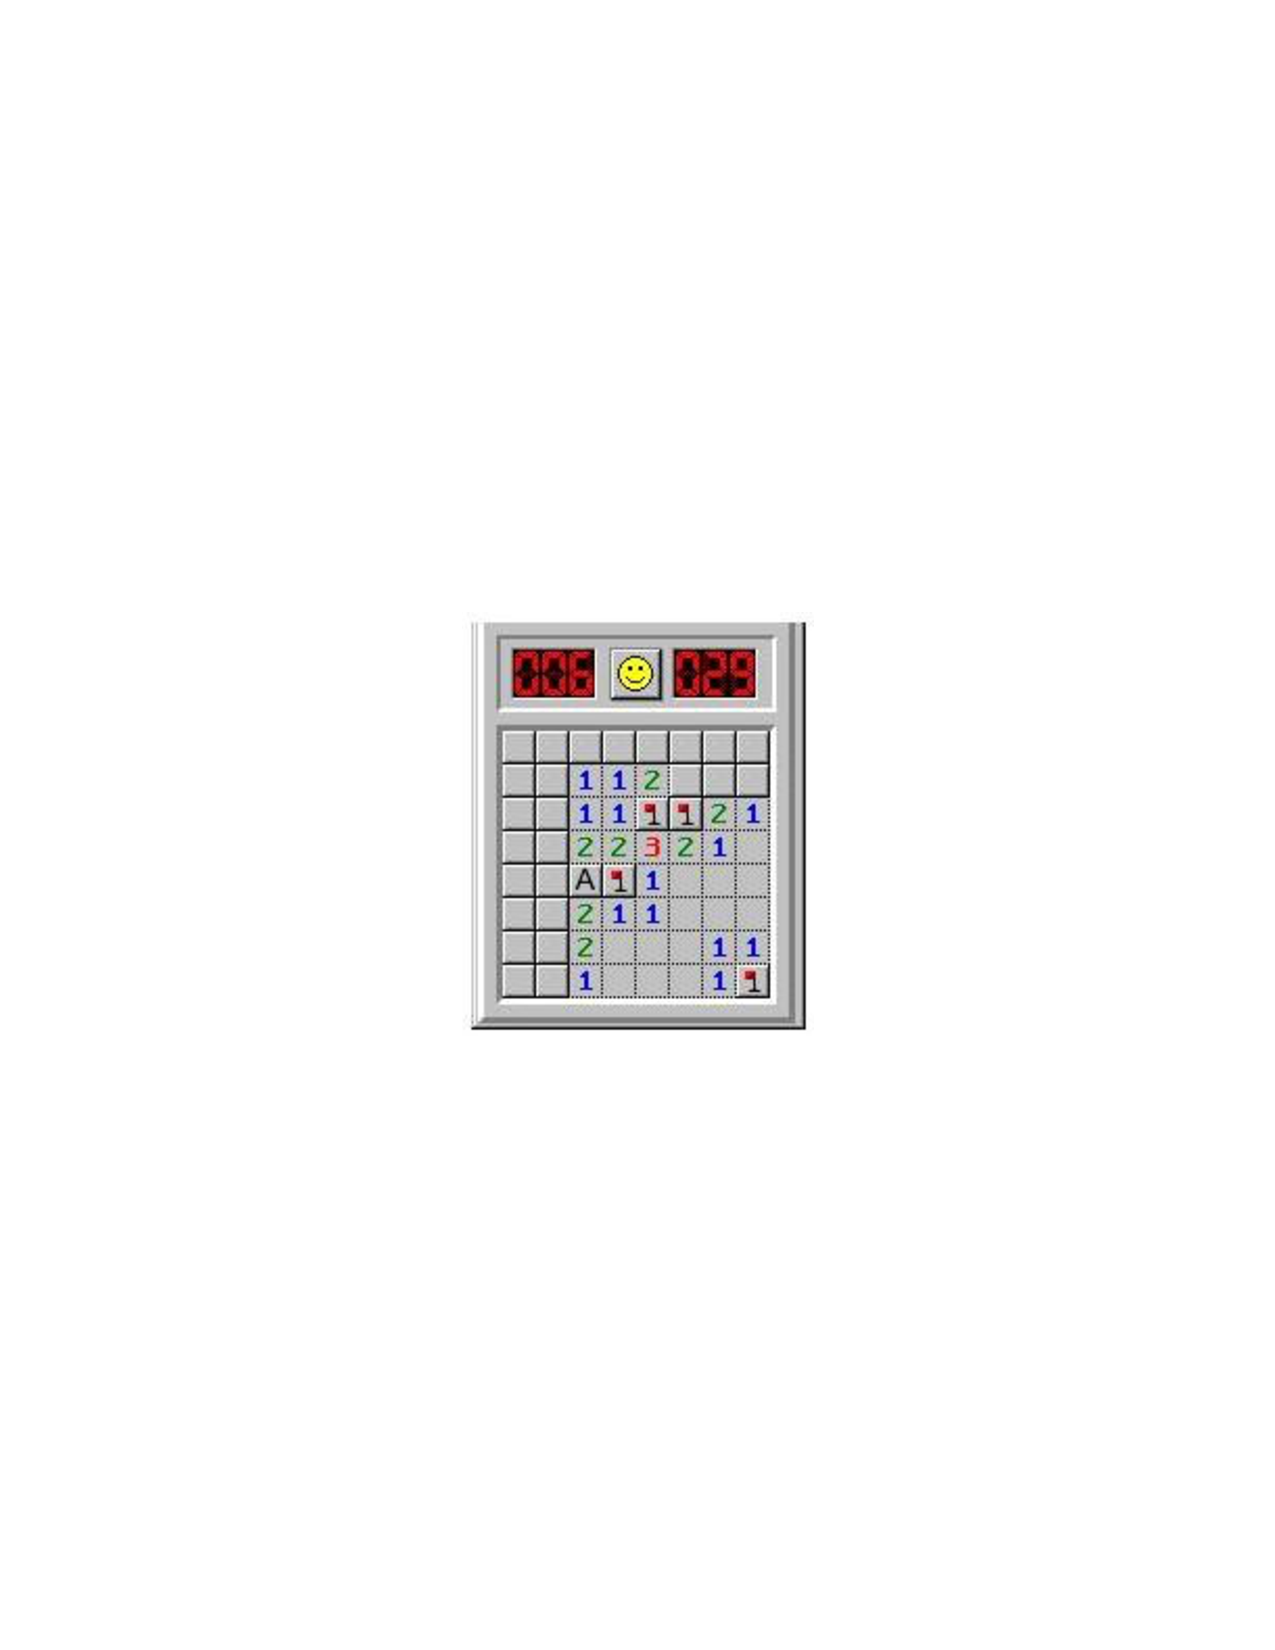
\includegraphics[width=2in]{images/minesweeper1.pdf}

\noindent \textbf{Sample Question:} Determine whether the following statement is true or false and explain. Square A is a mine.

\noindent \textbf{Sample Answer:} FALSE. The square directly below the flag next to the A contains a $1$, indicating that one and only one square adjacent to it is a mine. Since the square above the $1$ (the flag) is a mine, square A must not be a mine. We can conclude that the statement ``Square A is a mine." is false.

%<*truthTables:Minesweeper:entrance:game>
Consider the in-progress game below and determine if each statement below is true or false. Provide a brief justification for your claim.
\par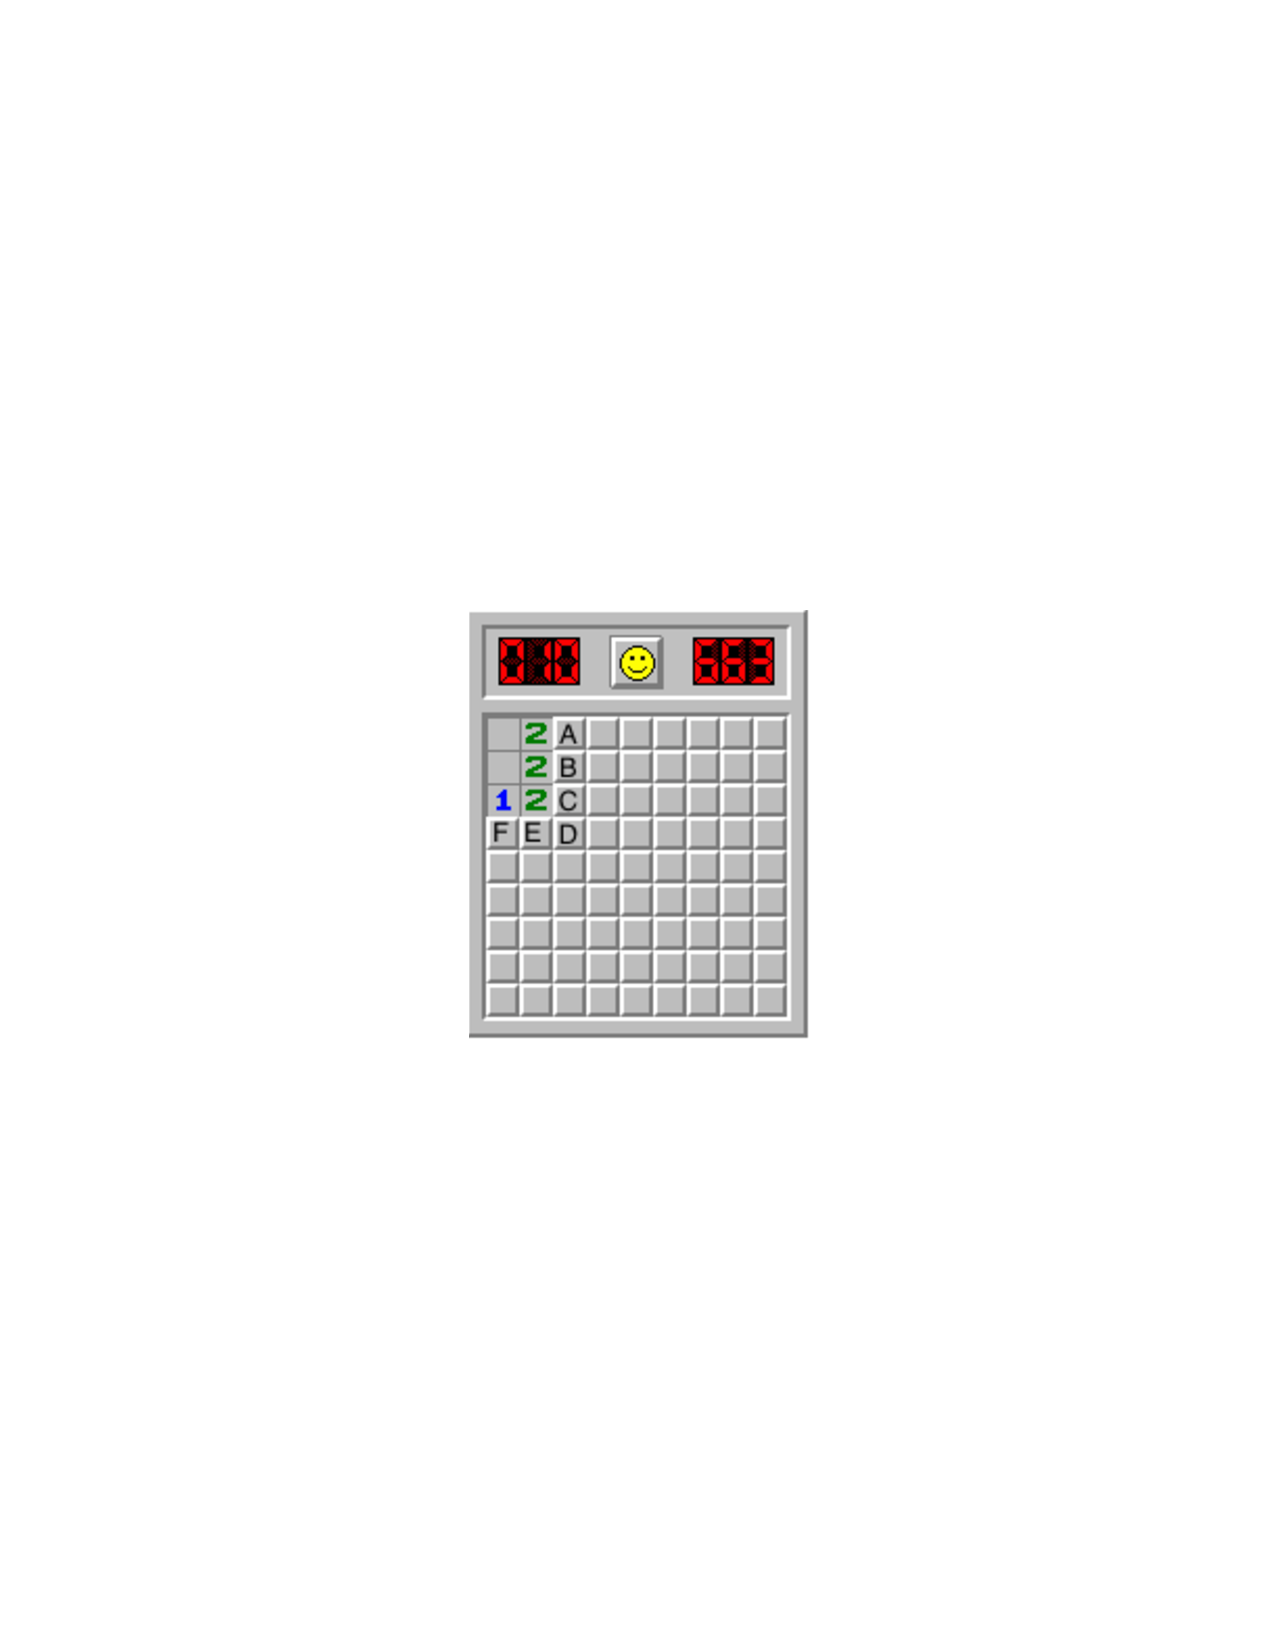
\includegraphics[width=2in]{images/MinesweeperBegin.pdf}
    \begin{enumerate}
        \item Squares A and B are mines.
        \par\Instr{ TRUE. The 2 next to the A requires two adjacent mines, and there are exactly 2 adjacent spaces that have not yet been cleared. Those are squares A and B, so A and B must be the two mines.}
        \wbvfill
        \item Square C is a mine
        \par\Instr{ FALSE. The 2 next to the B requires two adjacent mines. Since squares A and B are mines and are both adjacent, there must be no more mines adjacent to that 2. Since C is adjacent to the 2 also, it cannot be a mine.}
        \wbvfill
        \item Squares F and E are mines
        \par\Instr{ FALSE. There can only be one mine adjacent to the square above F. Since both E and F are adjacent to this square, they cannot both be mines.}
        \wbvfill
        \item Square D is a mine.
        \par\Instr{ FALSE. Squares B,E,F are all adjacent to the 2 above the E. B is a mine and exactly one of E and F is a mine due to the $1$ above the F. Either way, D cannot be a mine since that would place a third mine adjacent to the 2 above the E.}
        \wbvfill
    \end{enumerate}

\newpage
\subsection{Implications in Minesweeper}

In the game Minesweeper sometimes we cannot determine whether a square is a mine or not at first glance. If we can determine the state of a nearby square, however, that may help us figure it out. Here we wish to explore these scenarios and how logic plays a roll in beating the game.

\begin{enumerate}
\item \label{Minesweeper1} Consider this portion of an in-progress game. Are the statements below true, false, or indeterminate (need more information)? Explain.
\par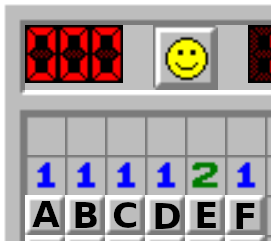
\includegraphics[width=2.5in]{images/MinesweeperImplication01.png}
\begin{enumerate}
    \item A is a mine.
    \par\Instr{ INDETERMINATE. Technically this is a TRUE statement, but it requires a lengthy argument (to be made forthwith). Without looking ahead or going through the investigation, the most likely and appropriate answer is indeterminate.}
    \wbvfill
    \item B is a mine.
    \par\Instr{ INDETERMINATE. Technically this is a FALSE statement, but it requires a lengthy argument (the same one that leads to the conclusion that A is a mine). Without looking ahead or going through the investigation, the most likely and appropriate answer is indeterminate.}
    \wbvfill
    \item \label{Minesweeper1.1} A is a mine or B is a mine.
    \par\Instr{ TRUE. A and B are both adjacent to the leftmost one, so at least one of them must be a mine. Of course the $1$ means exactly one of them must be a mine, but to state that A or B is true is to say that one or the other or both are true (that is, at least one is a mine is all that is needed).}
    \wbvfill
    \item \label{Minesweeper1.2} A is a mine and B is a mine.
    \par\Instr{ FALSE. A and B are both adjacent to the leftmost one, so they cannot both be mines. The combination of this statement being false and the previous statement being true leads to the conclusion (or is the logically equivalent statement) that exactly one of A and B is a mine.}
    \wbvfill
\end{enumerate}
    
\item \label{Minesweeper2} What can we conclude from the exploration in question \ref{Minesweeper1}? Circle one and explain.
\begin{enumerate}
    \item Neither A nor B is a mine.
    \item Both A and B are mines.
    \item Either A is a mine or B is a mine, but not both.
\end{enumerate}
\par\Instr{ From \ref{Minesweeper1.1} and \ref{Minesweeper1.2} (or from the fact that A and B are adjacent to the leftmost $1$), we conclude "Either A is a mine or B is a mine, but not both."}
\wbvfill

\wbnewpage
\item \label{Minesweeper3} So which is it? Is A the mine? or is B? To figure this out logically, we make A a mine and see what happens. So suppose A is a mine (as if we knew this to be a fact) and determine whether the following statements are true or false.
\begin{enumerate}
    \item If A is a mine, then B is clear.
    \par\Instr{ TRUE. The leftmost $1$ requires exactly one of A and B to be a mine.}
    \wbvfill
    \item If A is a mine, then B is clear and C is clear.
    \par\Instr{ TRUE. C must also be clear because the $1$ above the B is adjacent to both A and C so exactly one of them must be a mine (and we have assumed it is A).}
    \wbvfill
    \item If A is a mine, then B is clear and C is clear and D is a mine.
    \par\Instr{ TRUE. The $1$ above C is adjacent to B,C,D. Since B and C are clear, D must be the mine.}
    \wbvfill
    \item If A is a mine, then B is clear and C is clear and D is a mine and E is a mine and F is a mine.
    \par\Instr{ FALSE. The $1$ above D is adjacent to C,D,E. Since D is a mine, E must not be.}
    \wbvfill
    \item If A is a mine, then B is clear and C is clear and D is a mine and E is a mine and F is clear.
    \par\Instr{ FALSE. The $1$ above D is adjacent to C,D,E. Since D is a mine, E must be clear.}
    \wbvfill
    \item If A is a mine, then B is clear and C is clear and D is a mine and E is clear and F is a mine.
    \par\Instr{ TRUE. The 2 above E is adjacent to D,E,F. Since E is clear, F must be a mine.}
    \wbvfill
    \item If A is a mine, then B is clear and C is clear and D is a mine and E is clear and F is clear.
    \par\Instr{ FALSE. The 2 above E is adjacent to D,E,F. Only one of these squares is clear.}
    \wbvfill
\end{enumerate}
Now suppose B is a mine (as if we knew this to be a fact) and start over, assuming we don't know anything about any other square to begin. Determine whether the following statements are true or false.
\begin{enumerate}
    \item If B is a mine, then A is clear.
    \par\Instr{ TRUE. The leftmost $1$ requires exactly one of A and B to be a mine.}
    \wbvfill
    \item If B is a mine, then A is clear and C is clear.
    \par\Instr{ TRUE. C must also be clear because the $1$ above the B is adjacent to both B and C so exactly one of them must be a mine (and we have assumed it is B).}
    \wbvfill
    \item If B is a mine, then A is clear and C is clear and D is clear.
    \par\Instr{ TRUE. The $1$ above C is adjacent to B,C,D. Since B is a mine, D must be clear.}
    \wbvfill
    \item If B is a mine, then A is clear and C is clear and D is clear and E is a mine and F is a mine.
    \par\Instr{ FALSE. The $1$ above the F requires that only one of E and F be a mine.}
    \wbvfill
    \item If B is a mine, then A is clear and C is clear and D is clear and E is a mine and F is clear.
    \par\Instr{ FALSE. The 2 is adjacent to D,E,F. Since D is clear, F cannot also be clear.}
    \wbvfill
    \item If B is a mine, then A is clear and C is clear and D is clear and E is clear and F is a mine.
    \par\Instr{ FALSE. The 2 is adjacent to D,E,F. Since D is clear, E cannot also be clear.}
    \wbvfill
    \par\Instr{ FALSE. The 2 is adjacent to D,E,F. Since D is clear, F cannot also be clear.}
    \wbvfill
\end{enumerate}

\wbnewpage
\item \label{Minesweeper4} According to your answers in question \ref{Minesweeper3}, which do you think is the mine? A or B? Explain.
\par\Instr{ By contradiction, B cannot be the mine. There is no way to properly label squares A-F assuming B is a mine. Therefore A must be the mine. Since we have not formally discussed contradiction, however, students may not think this way. They may just have a hunch. Nudge them in the direction of understanding the contradiction, but don't get stuck on this. Let them proceed to the final question where it will be laid out.}
\wbvfill

\item \label{Minesweeper5} Below is more of the board from question \ref{Minesweeper1}. Use this new information to determine whether each square A through J is a mine or is clear. A board without the letters is supplied for you to work on. You may want to use a pencil!
\par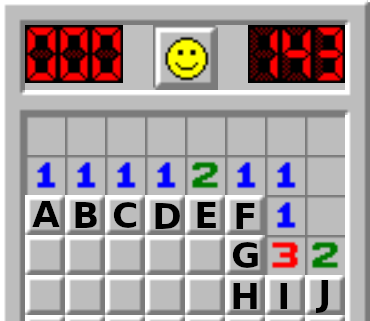
\includegraphics[width=3in]{images/MinesweeperImplication02.png}
\par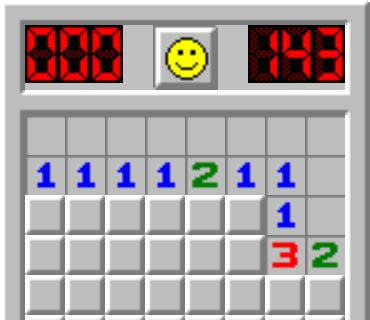
\includegraphics[width=3in]{images/MinesweeperImplication03.png}
\par\Instr{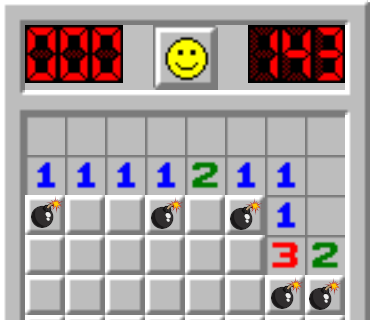
\includegraphics[width=3.25in]{images/MinesweeperImplication03-solved.png}}
\par Were you right about squares A and B?
\wbvfill

\wbnewpage
\item \label{Minesweeper6} Consider the in-progress game below. Are the following statements true or false? Explain.
\par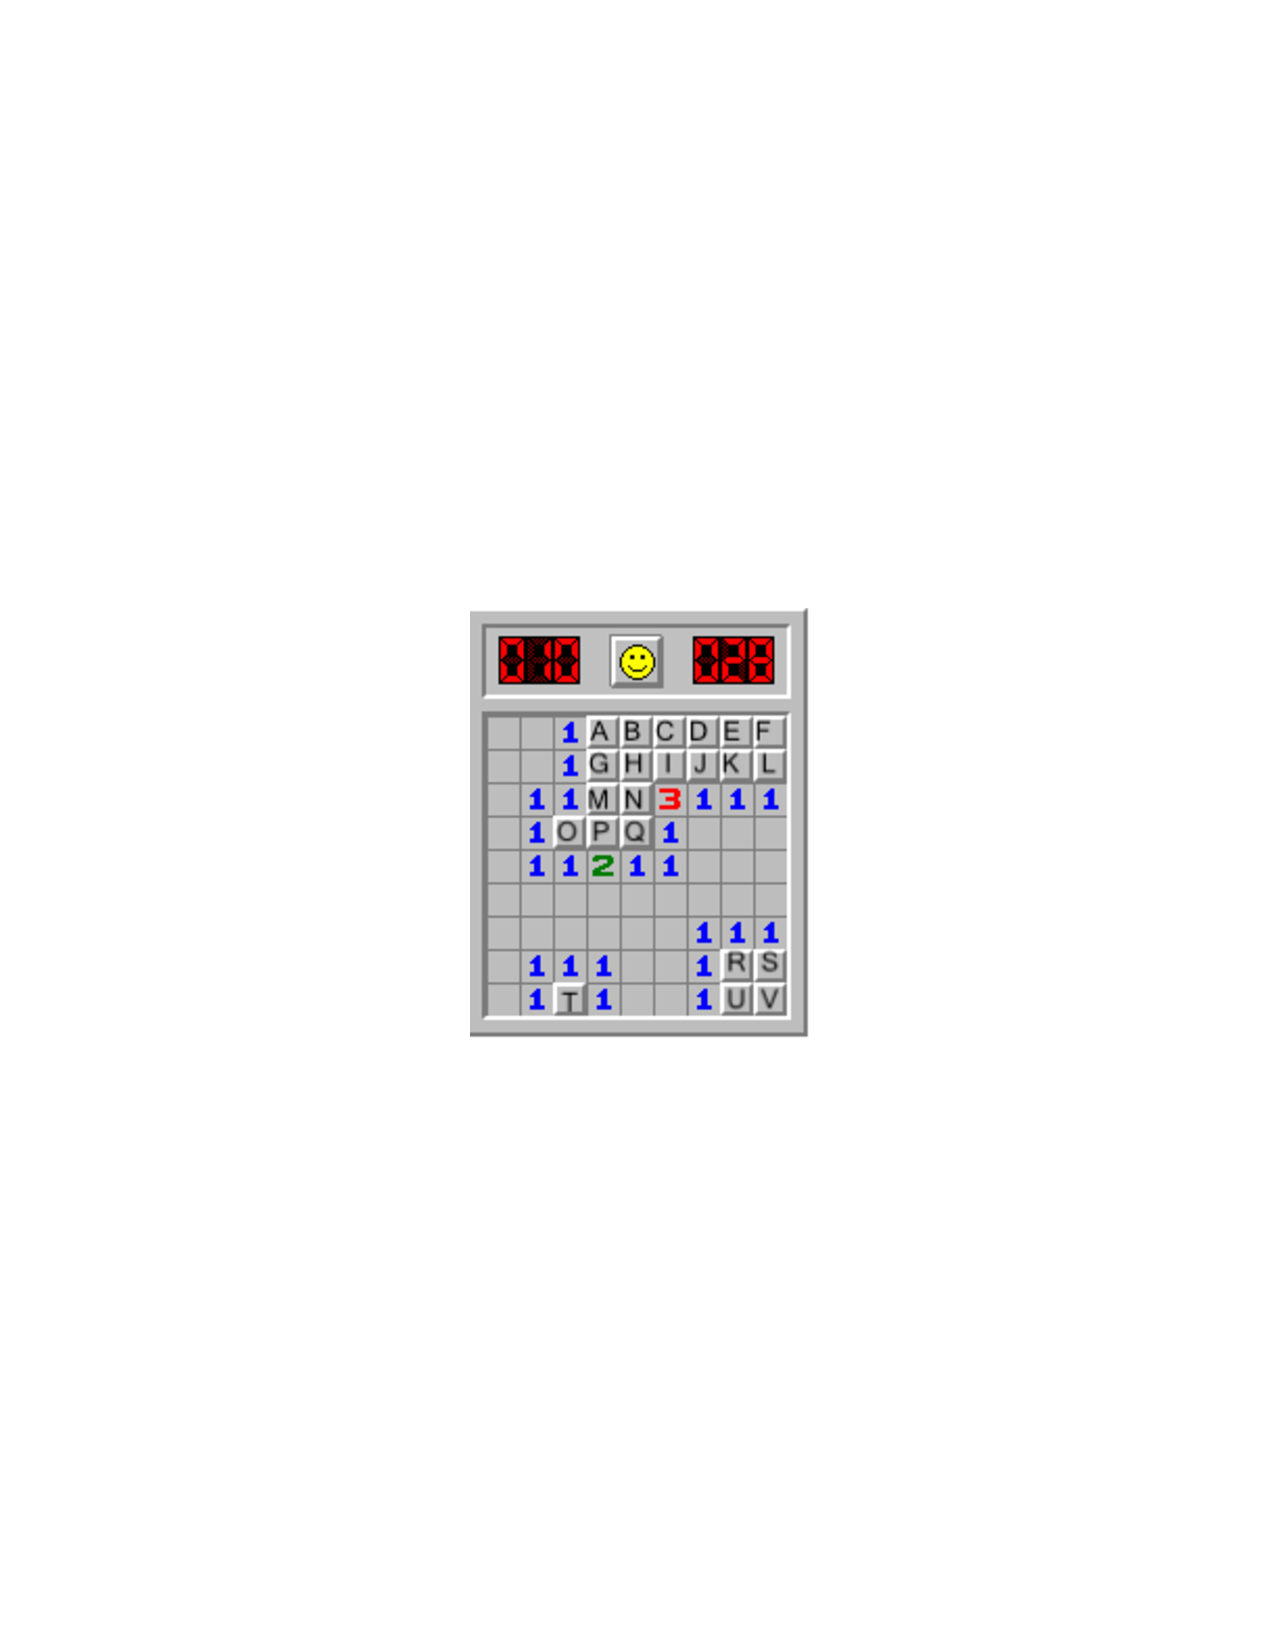
\includegraphics[width=2in]{images/MinesweeperArgument.pdf}
\begin{enumerate}
\item Square Q is a mine.
\par\Instr{ TRUE. The $1$ down and to the right of Q requires an adjacent mine. Since Q is the only uncleared adjacent space it must be the mine.}
\wbvfill
\item Square N is a mine.
\par\Instr{ FALSE. The $1$ next to the Q is, of course, adjacent to the Q. Since Q is a mine, no other space adjacent to the $1$ can be a mine. N is such a space and therefore cannot be a mine.}
\wbvfill
\item Square I is a mine and square J is a mine.
\par\Instr{ FALSE. I and J are both adjacent to the $1$ below J. Therefore they cannot both be mines.}
\wbvfill
\item Square H is a mine.
\par\Instr{ TRUE. The 3 requires three adjacent mines. One of them is at Q. One more is at I or J. N is not a mine. The only other adjacent uncleared square is H, and therefore must be a mine.}
\wbvfill
\item \label{KorL1} Square K is a mine or square L is a mine.
\par\Instr{ TRUE. The $1$ below the L requires it as K and L are the only adjacent uncleared squares.}
\wbvfill
\item \label{KorL2} If square K is a mine, then square J is not a mine.
\par\Instr{ TRUE. J and K are both adjacent to the $1$ under K. Therefore at most one of them can be a mine.}
\wbvfill
\item \label{KorL3} If square L is a mine, then square J is not a mine.
\par\Instr{ TRUE. J and L are both adjacent to the $1$ under K. Therefore at most one of them can be a mine.}
\wbvfill
\item Square J is not a mine.
\par\Instr{ TRUE. Statements \ref{KorL1},\ref{KorL2},\ref{KorL3} prove this. Either K or L is a mine [\ref{KorL1}], and either way J is not a mine [\ref{KorL2},\ref{KorL3}].}
\wbvfill
\end{enumerate}

\wbnewpage
\item Below is an argument table showing that the statement ``Square A is a mine'' is true for the game shown in question \ref{Minesweeper6}.
\begin{table}[htb]
    \centering
    \begin{tabular}{|l|p{3in}|}
        \hline
         True Statement & Reason \\
         \hline
         O is a mine & O is the only uncleared square adjacent to the $1$ on its left.\\
         \hline
         G is not a mine. & G is adjacent to the $1$ above the O (which is a mine).\\
         \hline
         A is a mine or G is a mine & A and G are the only uncleared squares adjacent to the $1$ next to A.\\
         \hline
         A is a mine. & The second and third rows (of this table) prove A is a mine.\\
         \hline
    \end{tabular}
    \caption{Argument}
    \label{tab:my_label}
\end{table}
Create an argument table for each statement below. You may use the statements in question \ref{Minesweeper6}, and you may bring in new statements as needed.
\begin{enumerate}
    \item Square P is not a mine.
    \wbvfill
	\Instr{ Here is a sample argument table. Students may resist actually writing the table since "it's so easy", but they should be encouraged to write it out for practice, and because what we are really learning here is the exposition of an argument, not just whether they "get it". Can they explain it in clear and concise language? The next exercise is not so easy.
	\begin{table}[htb]
    \centering
    \begin{tabular}{|l|p{3in}|}
        \hline
         True Statement & Reason \\
         \hline
         O is a mine & O is the only uncleared square adjacent to the $1$ on its left.\\
         \hline
         P is not a mine. & P is adjacent to the $1$ below the O (which is a mine).\\
         \hline
    \end{tabular}
    \caption{Sample Argument}
    \label{tab:my_label}
	\end{table}
	}
    \item Square I is a mine.
	\Instr{ Here is a sample argument table. Students are likely to skip writing much of the first several lines since they "are already done", but they should be encouraged to include them for sake of a complete, self-contained argument.
	\begin{table}[htb]
    \centering
    \begin{tabular}{|l|p{3in}|}
        \hline
         True Statement & Reason \\
         \hline
         Q is a mine & O is the only uncleared square adjacent to the $1$ below and to its right.\\
         \hline
         N is not a mine. & Q and N are adjacent to the $1$ next to Q. Since Q is a mine, N is not.\\
         \hline
         K is a mine or L is a mine & K and L are the only uncleared squares adjacent to the $1$ below L.\\
         \hline
         If K is a mine, then J is not a mine & J and K are both adjacent to the $1$ under K.\\
         \hline
         If L is a mine, then J is not a mine & J and L are both adjacent to the $1$ under K.\\
         \hline
         J is not a mine & The previous three lines in this table prove J is not a mine.\\
         \hline
         I is a mine & There are 5 uncleared squares adjacent to the 3: Q,N,H,I, and J. Since N and J are not mines, the other three must be, including I.\\
         \hline
    \end{tabular}
    \caption{Sample Argument}
    \label{tab:my_label}
	\end{table}
	}
    \wbvfill
\end{enumerate}
\end{enumerate}
\newpage


\subsection{Exit Slip}

For the in-progress game below, create three true statements, one for each type listed below.

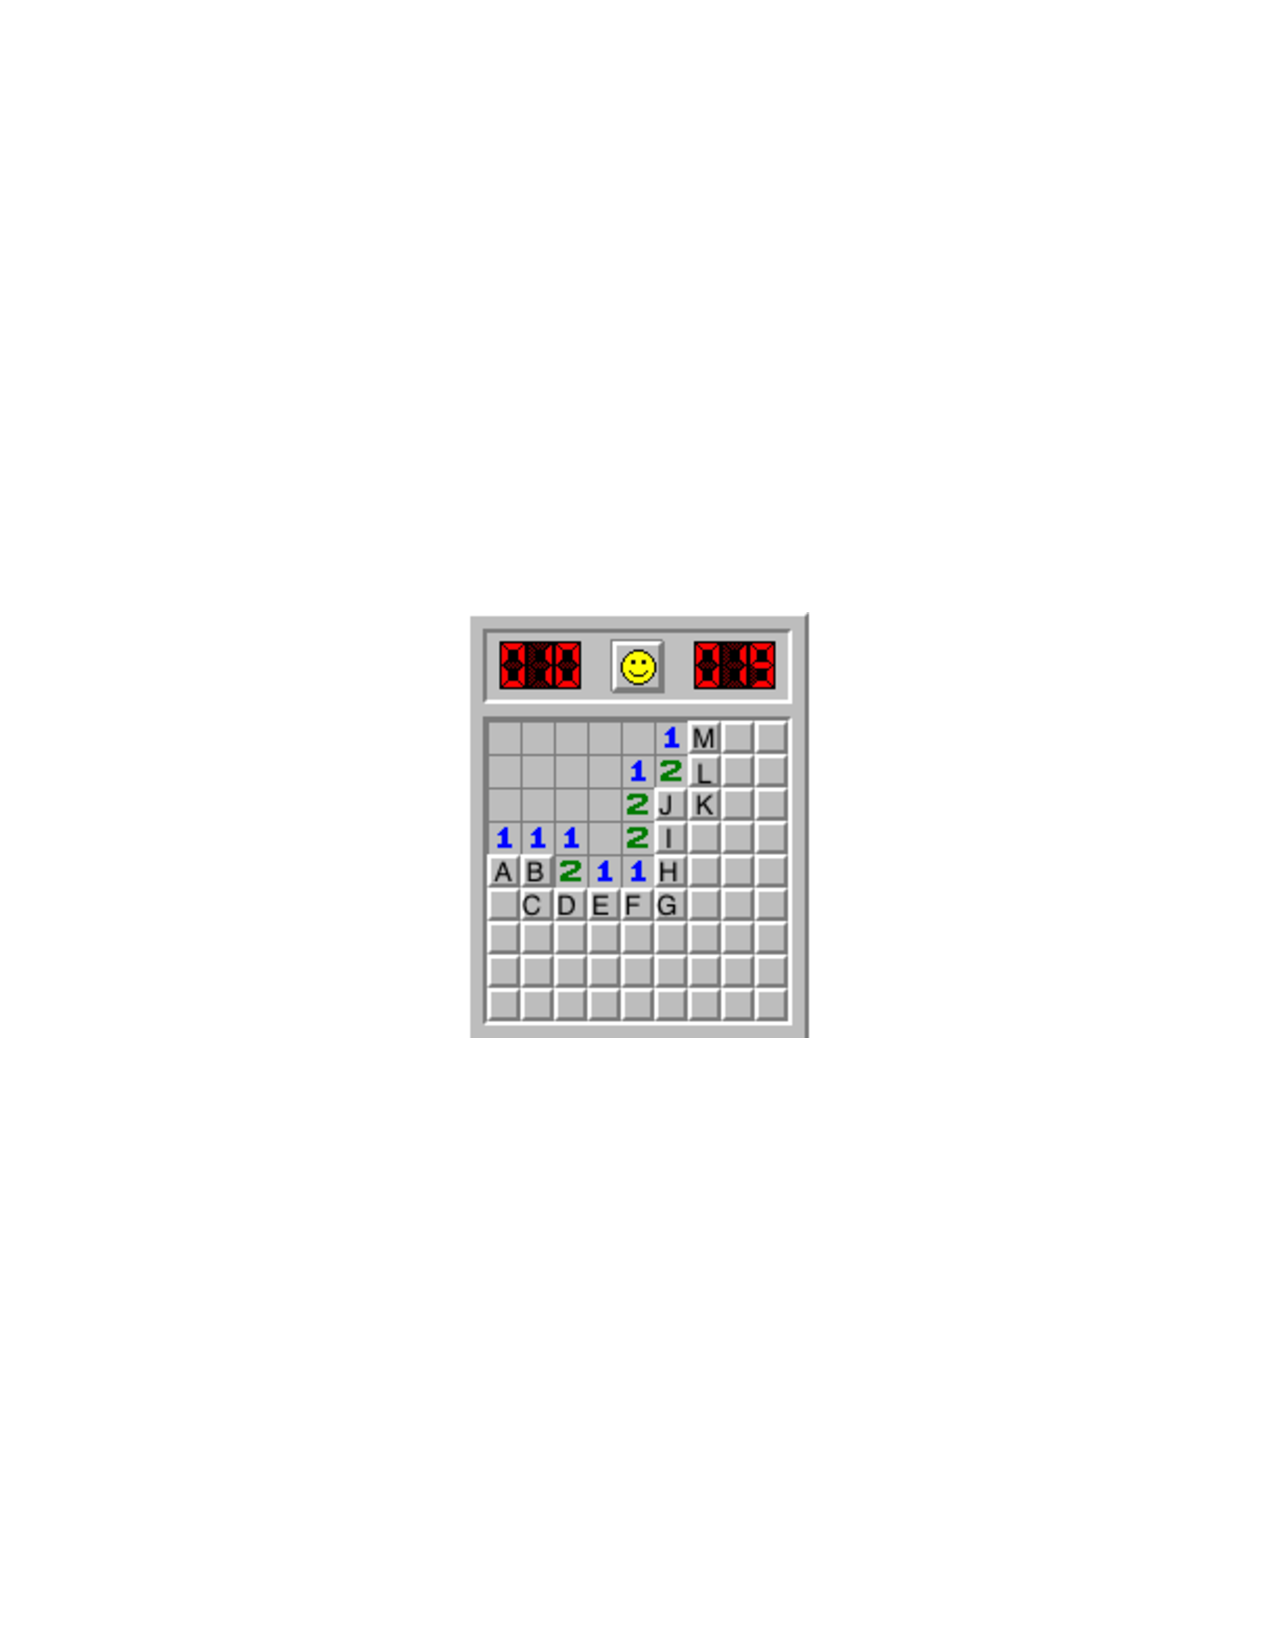
\includegraphics[width=3in]{images/MinesweeperExit.pdf}

\begin{enumerate}
    \item Statement containing an ``and''
    
    \item Statement containing an ``or''
    
    \item An implication statement in the form `` If \dots, then \dots.''
\end{enumerate}
\wbnewpage


\iffalse
%<*truthTables:statement:negation:intro>
\subsection{Activity: Negation}\label{negation}
%</truthTables:statement:negation:intro>

\Instr{  
Goals for this activity:
\begin{packedItem}
\item Working with negations withing compound statements; 
\item Determining truth values of compound statements containing negations; 
\item Completing Truth Tables for compounstatements containing negations; and
\item Determining weather two statements are equivalent.
\end{packedItem}
}

%<*truthTables:statement:negation:intro2>
\indent Let $\neg P$ represent the statement\index{statement} ``$P$ is false''. ($\neg P$\index{$\neg$} is called the negation of $P$.) Again we will consider the statements below.
\begin{center}
\begin{tabular}{ll}
$P$: & I am wearing a top hat.\\
$Q$: & I am wearing overalls.\\
$R$: & I am wearing rain boots.\\
\end{tabular}
\end{center}

\begin{enumerate}
\setcounter{enumi}{26}
\item\label{negPtrue} If $\neg P$ is true, is anything on my head? 
%</truthTables:statement:negation:intro2>

\Instr{  When $\neg P$ is true, ``$P$ is false'' is true, so I am not wearing a top hat. So there maybe something on my head, but it is not a top hat!}

%<*truthTables:statement:negation:negPtrue>
\item If $\neg P$ is false, is anything on my head?
%</truthTables:statement:negation:negPtrue>

\Instr{  When $\neg P$ is false, ``$P$ is false'' is false, so $P$ is true. Therefore there is something on my head when $\neg P$ is false, namely a top hat.}

%<*truthTables:statement:negation:negPfalse>
\item Fill in the truth table\index{truth table} below. Each cell in the table should contain either ``True'' or ``False.'' As in Question~{\normalfont\ref{logicTable}} begin by completing the first column.
\begin{center}
\begin{tabular}{|c||c|}
\hline
$P$ & $\neg P$ \\
\hline
\hline
\hspace{.75in} & \hspace{.75in} \\
\hline
& \\
\hline
\end{tabular}
\end{center}
%</truthTables:statement:negation:negPfalse>

\Instr{  
\begin{center}
\begin{tabular}{|c||c|}
\hline
$P$ & $\neg P$ \\
\hline
\hline
True & False \\
\hline
False & True \\
\hline
\end{tabular}
\end{center}
}

%<*truthTables:statement:negation:PwedgeRfalse>
\item Suppose you know the statement $P\wedge R$\index{$\wedge$} is false. Describe what I'm wearing. Is there a statement that says the same thing when it is true?
%</truthTables:statement:negation:PwedgeRfalse>

\Instr{  If $P\wedge R$ is false then it is not the case that I am wearing both a top hat and rain boots. Therefore I am either ``not wearing a top hat'' or ``I am not wearing rain boots.'' The easiest way to find a corresponding true statement is to simply apply the $\neg$ function and use $\neg (P\wedge R)$. But the verbal description of what I'm wearing leads to another solution: $\neg P \vee \neg Q$\index{$\neg$}\index{$\vee$}. Encourage the students to find both answers.}

%<*truthTables:statement:negation:QveeRfalse>
\item Suppose you know the statement $Q\vee R$ is false. Describe what I'm wearing. Is there a statement\index{statement} that says the same thing when it is true?
%</truthTables:statement:negation:QveeRfalse>

\Instr{  If $Q\vee R$ is false then it is not the case that either I am wearing overalls or I am wearing rain boots. So I cannot be wearing either. Therefore I am not wearing overalls and I am not wearing rain boots. So both the statement\index{statement} $\neg Q \wedge \neg R$\index{$\neg$}\index{$\wedge$} is true. What I am wearing is also described by $\neg(Q\wedge R)$, as can be seen by applying the definition of $\neg$. So both are good answers.}

%<*truthTables:statement:negation:PwedgenegQfalse>
\item Suppose you know that statement $P\wedge \neg Q$ is false. Describe what I'm wearing. Is there a statement that says the same thing when it is true?
%</truthTables:statement:negation:PwedgenegQfalse>

\Instr{  If $P\wedge \neg Q$ is false then it is not the case that I am both wearing a top hat and not wearing overalls. Therefore either I am not wearing a top hat or I am wearing overalls. So the statement\index{statement} $\neg P\vee Q$\index{$\neg$}\index{$\vee$}\index{$\wedge$} is true. Also, $\neg(P\wedge \neg Q)$ is true by the definition of $\neg$. So both are good answers.}

%<*truthTables:statement:negation:logicTable2.5>
\item\label{logicTable2.5} Fill in the truth table\index{truth table} below so that each cell contains either ``True'' or ``False.'' As in Question~{\normalfont\ref{logicTable}}, begin by completing the first two columns so that all ways truth values can be assigned to $P$ and $Q$ are represented in the four rows.
\begin{center}
\begin{tabular}{|c|c||c|c|c|c|}
\hline
$P$ & $Q$ & $\neg P$ & $\neg Q$ & $\neg(P\wedge Q)$ & $\neg P\vee \neg Q$ \\
\hline
\hline
\hspace{.5in} & \hspace{.5in} & \hspace{.5in} & \hspace{.5in} & \hspace{.75in} & \hspace{.75in} \\
\hline
&&&&& \\
\hline
&&&&& \\
\hline
&&&&& \\
\hline
\end{tabular}
\end{center}
%</truthTables:statement:negation:logicTable2.5>

\Instr{ 
\begin{center}
\begin{tabular}{|c|c||c|c|c|c|}
\hline
$P$ & $Q$ & $\neg P$ & $\neg Q$ & $\neg (P\wedge Q)$ & $\neg P\vee \neg Q$ \\
\hline
\hline
True & True & False & False & False & False  \\
\hline
True & False & False & True & True & True  \\
\hline
False & True & True & False & True & True \\
\hline
False & False & True & True & True & True \\
\hline
\end{tabular}
\end{center}
}

%<*truthTables:statement:negation:sameStatement?>
\item Using the truth table\index{truth table} in Question~{\normalfont\ref{logicTable2.5}} determine if the statement $\neg(P\wedge R)$ is the same as the statement\index{statement}\index{$\wedge$}\index{$\vee$}\index{$\neg$} $\neg P \vee \neg R$. Explain yourself thoroughly.
%</truthTables:statement:negation:sameStatement?>

\Instr{  Based on the truth table they are the same. Also, by reasoning out what each of the statements is saying, it is clear that the two statements are identical.}

%<*truthTables:statement:negation:logicTable3>
\item\label{logicTable3} Fill in the table below so that each cell contains either ``True'' or ``False.'' As in Question~{\normalfont\ref{logicTable}}, begin by completing the first two columns.
\begin{center}
\begin{tabular}{|c|c||c|c|c|c|c|}
\hline
$P$ & $Q$ & $\neg P$ & $\neg Q$ & $\neg P\wedge Q$ & $P\vee \neg Q$ & $\neg P\vee \neg Q$ \\
\hline
\hline
\hspace{.5in} & \hspace{.5in} & \hspace{.5in} & \hspace{.5in} & \hspace{.75in} & \hspace{.75in} & \hspace{.75in} \\
\hline
&&&&&& \\
\hline
&&&&&& \\
\hline
&&&&&& \\
\hline
\end{tabular}
\end{center}
%</truthTables:statement:negation:logicTable3>

\Instr{  
\begin{center}
\begin{tabular}{|c|c||c|c|c|c|c|}
\hline
$P$ & $Q$ & $\neg P$ & $\neg Q$ & $\neg P\wedge Q$ & $\neg P\vee \neg Q$ & $P\vee \neg Q$ \\
\hline
\hline
True & True & False & False & False & False & True \\
\hline
True & False & False & True & False & True & True \\
\hline
False & True & True & False & True & True & False \\
\hline
False & False & True & True & False & True & True \\
\hline
\end{tabular}
\end{center}
}

%<*truthTables:statement:negation:logicTable4>
\item\label{logicTable4} Fill in the table below so that each cell contains either ``True'' and ``False.'' As in Question~{\normalfont\ref{logicTable}}, begin by completing the first three columns.
\begin{center}
\begin{tabular}{|c|c|c||c|c|c|}
\hline
$P$ & $Q$ & $R$ & $(P\wedge Q) \wedge \neg R$ & $(\neg P \vee \neg Q) \vee R$ & $(P\vee \neg Q) \wedge \neg R$ \\
\hline
\hline
\hspace{.5in} & \hspace{.5in} & \hspace{.5in} &&& \\
\hline
&&&&& \\
\hline
&&&&& \\
\hline
&&&&& \\
\hline
&&&&& \\
\hline
&&&&& \\
\hline
&&&&& \\
\hline
&&&&& \\
\hline
\end{tabular}
\end{center}
%</truthTables:statement:negation:logicTable4>

\Instr{  
\begin{center}
\begin{tabular}{|c|c|c||c|c|c|}
\hline
$P$ & $Q$ & $R$ & $(P\wedge Q) \wedge \neg R$ & $(\neg P \vee \neg Q) \vee R$ & $(P\vee \neg Q) \wedge \neg R$ \\
\hline
\hline
True & True & True & False & True & False \\
\hline
True & True & False & True & False & True \\
\hline
True & False & True & False & True & False \\
\hline
True & False & False & False & True & True \\
\hline
False & True & True & False & True & False \\
\hline
False & True & False & False & True & False \\
\hline
False & False & True & False & True & False \\
\hline
False & False & False & False & True & True \\
\hline
\end{tabular}
\end{center}
}

%<*truthTables:statement:negation:negnegP>
\item Write out what it means if the statement\index{statement} $\neg (\neg P))$\index{$\neg$} is true.
%</truthTables:statement:negation:negnegP>

\Instr{  The statement $\neg(\neg P))$ means it is not the case that I am not wearing a top hat. In other words, I am wearing a top hat; so $P$ is true.}

%<*truthTables:statement:negation:end>
\end{enumerate}
%</truthTables:statement:negation:end>
\fi

%<*truthTables:conditional:title>
\section{Extension Activity: Arguments}

\subsection{Activity: Nancy Out On The Town}\label{conditional}
%</truthTables:conditional:title>

\Instr{  
Goals for this activity:
\begin{packedItem}
\item Discovering the implications of compound statements containing dependant statements; 
\end{packedItem}
}

%<*truthTables:conditional:intro>
\indent Nancy's friends are trying to find her based on whether the following statements\index{statement} are true or false. They know that she is at exactly one of: home, the movie theater, the grocery store, or a clothing store.
\begin{center}
\begin{tabular}{ll}
$P$: & Nancy is at home. \\
$Q$: & Nancy is at the movie theater. \\
$R$: & Nancy is at the grocery store. \\
$S$: & Nancy is at a clothing store. \\
$T$: & Nancy is trying on clothes. \\
$U$: & Nancy is buying food.
\end{tabular}
\end{center}

\begin{enumerate}
\item If $P$ is true is $Q$ true or false? Explain your reasoning.
%</truthTables:conditional:intro>

\Instr{  It is clear that someone can't be in two places at once. So your home cannot be at the movie theater and statement $Q$ is false.}\wbvfill

%<*truthTables:conditional:IfQthenP>
\item What statements could be true if $T$ is true? Explain your reasoning.
%</truthTables:conditional:IfQthenP>

\Instr{  If $T$ is true, then we must identify the locations where Nancy could possibly be. Those locations would be home or the clothing store. So one of $P$ and $S$ could be true.}\wbvfill

%<*truthTables:conditional:IfPthenQorR>
\item If $P$ is true, is $T\vee U$\index{$\vee$} true or false? Explain your answer.
%</truthTables:conditional:IfPthenQorR>

\Instr{  If $P$ is true, then Nancy is at home. She cannot buy food at home (unless she does so over the internet!), but she can be trying on clothes at home. Since we are using the ``or'' operator, the statement $T\vee U$ could be true, but may be false if at the moment she is doing other things like cooking dinner.
}\wbvfill

%<*truthTables:conditional:IfPthenNotS>
\item If $P$ is true, is $\neg S$\index{$\neg$} true or false? Explain your answer.
%</truthTables:conditional:IfPthenNotS>

\Instr{  Notice that $\neg S$ means that Nancy is not at the clothing store. Since she is at home, $\neg S$ is true in this case.}\wbvfill

%<*truthTables:conditional:IfQorRthenP>
\item What statements are false if $Q\vee R$ is true? 
%</truthTables:conditional:IfQorRthenP>

\Instr{  The statement $Q\vee R$ is true states that Nancy is at the movie theater or at the grocery store. So she cannot be at home, nor is she at the clothing store. She is also not trying on clothes. So $P$,  $S$, and $T$ are false.}\wbvfill

%<*truthTables:conditional:IfUthenQandR>
\item If $U$ is true, is $Q\wedge R$\index{$\wedge$} true or false? Explain your conclusion.
%</truthTables:conditional:IfUthenQandR>

\Instr{  If $U$ is true, then Nancy is buying food. It is possible to buy food at both the grocery store and the movie theater. So $Q\wedge R$ is true.} \wbvfill

%<*truthTables:conditional:IfPthenTrue>
\item If $U$ is false, what do you know must be false? Explain your answer.
%</truthTables:conditional:IfPthenTrue>

\Instr{  If Nancy is not buying food, then she cannot be at the grocery store. So $R$ is false. Students may find another reason to be at the grocery store--if you consider it a good reason then there are no statements\index{statement} that you know are definitely false.}\wbvfill

%<*truthTables:conditional:IfPtrueQfalse>
\item If $T$ is true and $U$ is false, what single true statement can you create concerning Nancy's location? Explain your results.
%</truthTables:conditional:IfPtrueQfalse>

\Instr{  If Nancy is trying on clothes and not buying food, then Nancy is either at home or at the clothing store. So the statement $P\vee S$\index{$\vee$} is true.}\wbvfill

%<*truthTables:conditional:QRST>
\item If $U$ is true, what single true statement can you create concerning Nancy's locations? Explain your results.
%</truthTables:conditional:QRST>

\Instr{  Since Nancy is buying food, Nancy is either at the movie theater or at the grocery store. So $Q\vee R$\index{$\vee$} is true. Some students may raise the issue of buying food on the internet making $P$ another possible answer. This is fine as long as the students explain themselves, in which case the answer would be $P\vee Q\vee R$.}\wbvfill

%<*truthTables:conditional:IfTtrue>
\item If $P$ is true and $Q$ is false, is $R\vee(T\wedge U)$\index{$\wedge$} true or false? Explain your results.
%</truthTables:conditional:IfTtrue>

\Instr{  Since Nancy is at home, Nancy is not at the grocery store (so $R$ is false) and cannot be buying food at her home (so $U$ is false), so $R\vee(T\wedge U)$ must be false. Even if students want to allow the possibility of buying food at home on the internet, it would be difficult (impossible?) to do so while trying on clothes, so $T\wedge U$ is false; so even in this case $R\vee(T\wedge U)$ is false.}\wbvfill

%<*truthTables:conditional:IfnegTtrue>
\item If $T$ is true, is $\neg Q \wedge(S\vee P)$\index{$\neg$} true or false? Why?
%</truthTables:conditional:IfnegTtrue>

\Instr{  Since Nancy is trying on clothes, she cannot be at the movie theater (so $\neg Q$ is true), nor is she at the grocery store. So she must be at home or the clothing store. So $\neg Q\wedge (S\vee P)$ is true.} \wbvfill
%<*truthTables:conditional:end>
\end{enumerate}
%</truthTables:conditional:end>

%<*truthTables:implications:title>


\wbnewpage

\section{Project Choices}
\Instr{ Students should complete one of the following projects.}
\begin{enumerate}
    \item \textbf{Project Question:} You are given an in-progress Minesweeper game. On the given board:
    \begin{enumerate}
        \item Mark each box adjacent to a numbered square with an O if it can be determined to be a mine or X if it can be determined that it is not a mine.
        \textit{* There are at least 3 squares that are mines and at least 3 squares that are not mines. There may also be squares adjacent to the numbers that cannot be determined. Leave them blank. *}
        \item Write an argument table for one of the squares marked with an O. \textit{* Do not pick a square located in a ``corner'' adjacent to a square with a $1$. *}
        \item Write an argument table for one of the squares marked with an X.
    \end{enumerate}
    
    \item \textbf{Project Question:} You are given an empty nonogram board. Your project is to do the following.
    \begin{enumerate}
        \item Fill all squares correctly, making note of your logic.
        \item Write one true statement using an ``and'' that helped you complete the puzzle.
        \item Write one true statement using an ``or'' that helped you complete the puzzle.
    \end{enumerate}
    The rules for filling the board are as follows.
    \begin{itemize}
        \item Each box must be filled in black or marked with X.
        \item Beside each row of the grid are listed the lengths of the runs of consecutive black squares on that row.
        \item Above each column are listed the lengths of the runs of consecutive black squares in that column. 
        \item Boxes that are not part of a run of black squares must be marked with X.
    \end{itemize}
    \wbnewpage
    Here is an example of a puzzle in progress.
    \begin{center}
        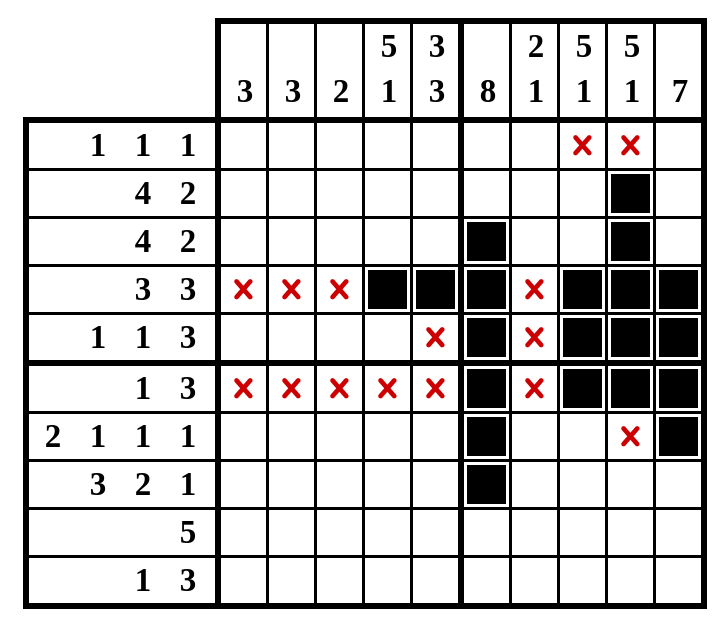
\includegraphics[width=5in]{images/nonogram00.png}
    \end{center}
    The four squares in the rightmost column were filled in first. 7 consecutive squares in that column must be filled in and there are only 10 squares total, so you can only skip three of them from the top \textbf{or} three of them from the bottom. The black squares and X's immediately to the left of those four were filled in next. For example, in row 4 the tenth square in that row is filled in \textbf{and} the last run of squares must be length 3, so the two squares next to the last one must also be filled in black. That completes the run so the square next to that (the 6th from the left in that row) must not be filled (so is marked with an X). See if you can figure out why the rest of the marked squares are the way they are.

    You may want to visit \href{https://www.puzzle-nonograms.com/}{https://www.puzzle-nonograms.com/} to try some nonogram puzzles at a variety of difficulty levels online.

    \item \textbf{Project Question:} You are given two KenKen puzzles. Your project is to do the following.
    \begin{enumerate}
        \item Fill all squares correctly in each puzzle, making note of your logic.
        \item Write one true statement using an ``and'' that helped you complete one of the puzzles.
        \item Write one true statement using an ``or'' that helped you complete one of the puzzles.
    \end{enumerate}
    The rules for solving a KenKen are as follows.
    \begin{itemize}
        \item The only numbers you may write are $1,2,3,\ldots$ up to the number of rows and columns. In a $4\times4$ puzzle you will use the numbers 1 through 4. In a $6\times6$ puzzle you will use the numbers 1 through 6, and so on.
		\item Every allowable number must appear in every row and every column. No number may be repeated in any row or any column.
		\item Each region bounded by a heavy border, called a \textbf{cage}, contains a target number and usually an arithmetic operation. You must fill that cage with numbers that reach the target using the specified arithmetic operation. Numbers may repeat within a cage, if needed, as long as they do not repeat within a single row or column.
    \end{itemize}
    Here is an example of a puzzle in progress.
    \begin{center}
        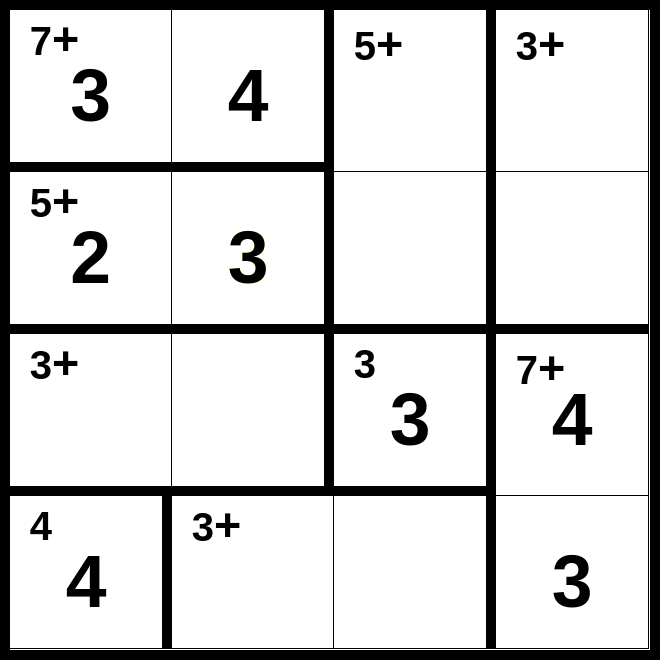
\includegraphics[width=2.5in]{images/kenken00.png}
    \end{center}
    Here is how the numbers were filled in to this point.

    \begin{tabular}{p{3.5in}p{2in}}
         \begin{itemize}\item The $4$ in the bottom left corner and the $3$ in the third row, third column were filled in first. Their cages are only one block so there is no operation to consider. The target number is the number that needs to be filled in.\end{itemize} & \raisebox{-2in}{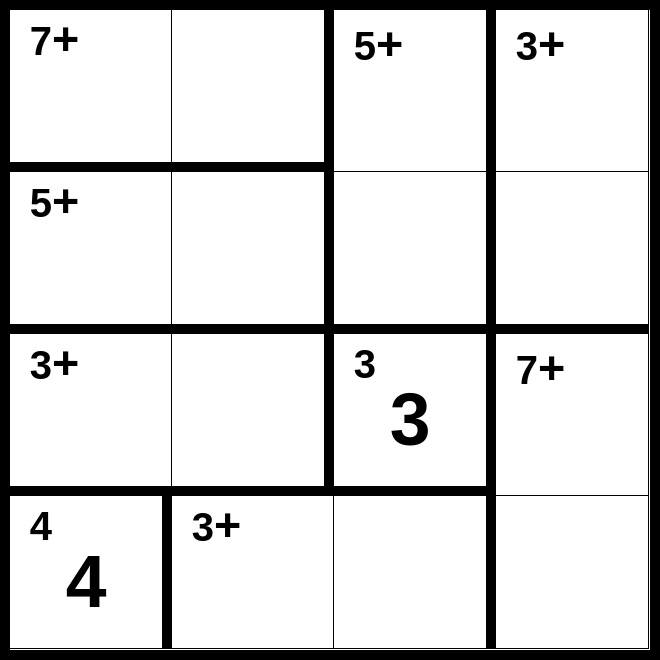
\includegraphics[width=1.9in]{images/kenken00-2.png}}\\
    \end{tabular}
    \begin{tabular}{p{3.5in}p{2in}}
         \begin{itemize}\item The two cages with $7+$ in them were filled in next. In each cage, the numbers $3$ and $4$ must be placed since the only way for two \textbf{different} numbers between 1 and 4 to add up to seven is to use $3$ and $4$. For the cage in the bottom right, the $4$ must be in the third row since there is already a $3$ in that row. You can come to the same conclusion by noticing there is a $4$ in the fourth row (bottom left corner) already, so the $4$ for this cage cannot be put in the fourth row. See if you can understand why the $3$ and $4$ in the $7+$ cage in the top left of the board were placed the way they were. They cannot be placed the other way around.\end{itemize} & \raisebox{-2in}{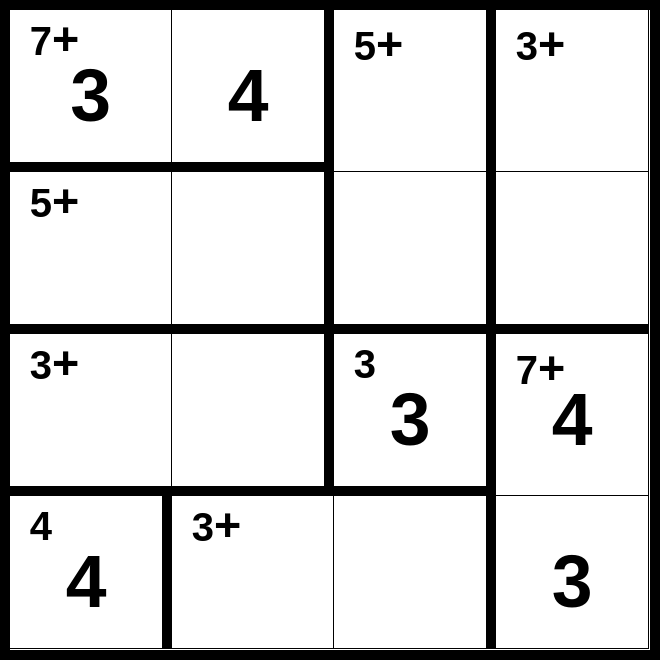
\includegraphics[width=1.9in]{images/kenken00-3.png}}\\
    \end{tabular}
    \begin{tabular}{p{3.5in}p{2in}}
         \begin{itemize}\item The $5+$ cage with the $2$ and $3$ in it was filled in next. There are two ways to use different numbers between 1 and 4 to sum to five---$1$ and $4$ or $2$ and $3$. However, there are already $4$'s in columns one and two, so a $4$ cannot be used in this cage. Hence the cage will be filled with $2$ and $3$. Since there is already a $3$ in column one, the $3$ for this cage must be in column two and therefore the $2$ must be in column one.\end{itemize} & \raisebox{-2in}{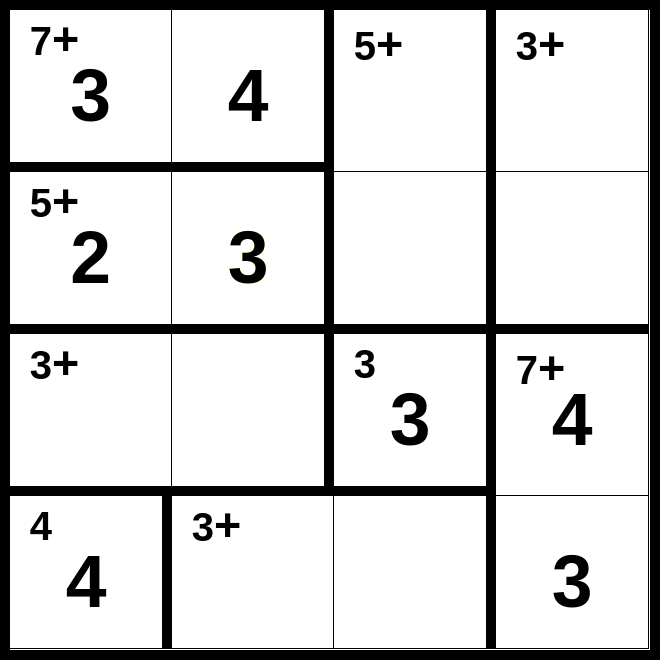
\includegraphics[width=1.9in]{images/kenken00.png}}\\
    \end{tabular}

    See if you can complete the puzzle. HINT: The first column already has the numbers $2,3,4$ in it. There is only one number that can be put in the empty box of that column!

    You may want to visit \href{https://www.kenkenpuzzle.com/}{https://www.kenkenpuzzle.com/} to try some KenKen puzzles at a variety of difficulty levels online. Begin by clicking the "Create Custom Puzzle" button.

    \item \textbf{Project Question:} You are given a Sudoku Pair Puzzle. This isn't your regular Sudoku though! Fully complete the puzzle and provide a paragraph description of how you used logic to complete the puzzle, using examples from your specific game.

	\textbf{(2,5) - Sudoku Pair Puzzle Rules}: Each completed puzzle is a 10 by 10 grid that contains exactly one integer from 1 to 10 in each cell. Furthermore, there are regions that must contain every integer exactly once. The regions are described below and outlined in the puzzle:
	\begin{enumerate}
		\item Each row is its own region.
		\item Each column is its own region.
		\item Each 2 by 5 rectangle outlined by bold lines is its own region.
		\item Each 5 by 2 rectangle outlined by dashed lines is its own region.
	\end{enumerate}
	\begin{center}
		Here is an example of a completed puzzle.\par
		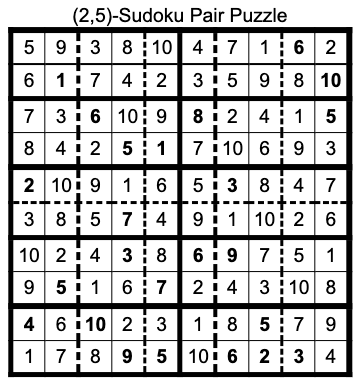
\includegraphics[width=4in]{images/SPPExample.png}
	\end{center}
	We've been describing $(2,5)$ Sudoku pair puzzles.  A slightly simpler example would be $(2,3)$ Sudoku pair puzzles.  It might be helpful to warm up on some of these! There is a webpage which will let you practice online:

	\href{http://www2.cedarcrest.edu/academic/math/jmhammer/SudokuWebapp/23SPLS/}{http://www2.cedarcrest.edu/academic/math/jmhammer/SudokuWebapp/23SPLS/}
\end{enumerate}

\Instr{ The following pages have Minesweeper games in progress, Nonogram boards, KenKen puzzles, and Sudoku Pair puzzles with answers.\newpage

    \begin{center}
        Minesweeper Project Game 1\par\bigskip
        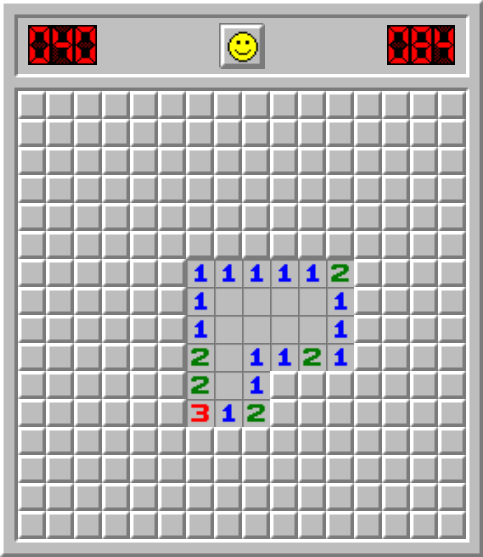
\includegraphics[width=5in]{images/MSProject1.png}
    \end{center}
    \newpage
    \begin{center}
        Minesweeper Project Game 2\par\bigskip
		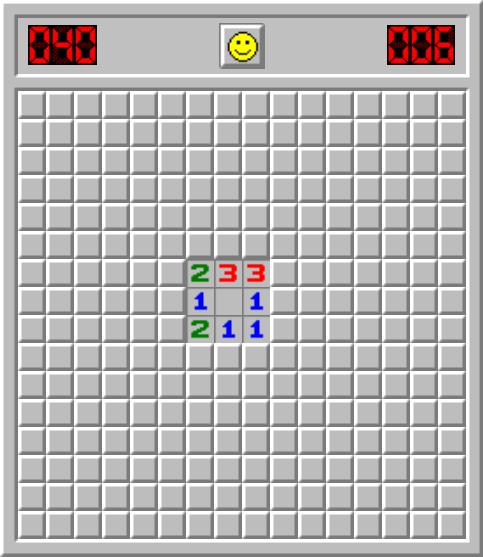
\includegraphics[width=5in]{images/MSProject2.png}
    \end{center}
    \newpage
    \begin{center}
        Minesweeper Project Game 3\par\bigskip
		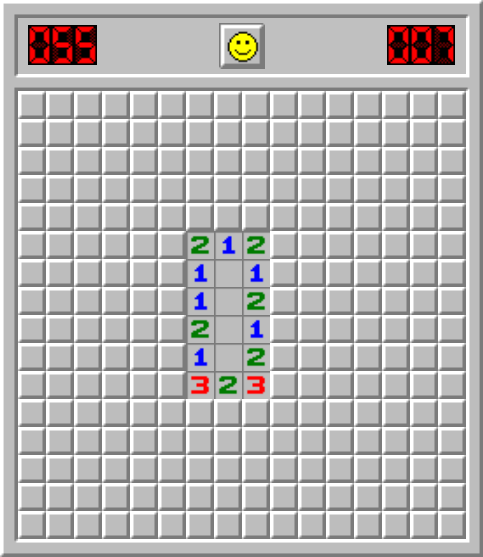
\includegraphics[width=5in]{images/MSProject3.png}
    \end{center}
    \newpage
    \begin{center}
        Minesweeper Project Game 4\par\bigskip
		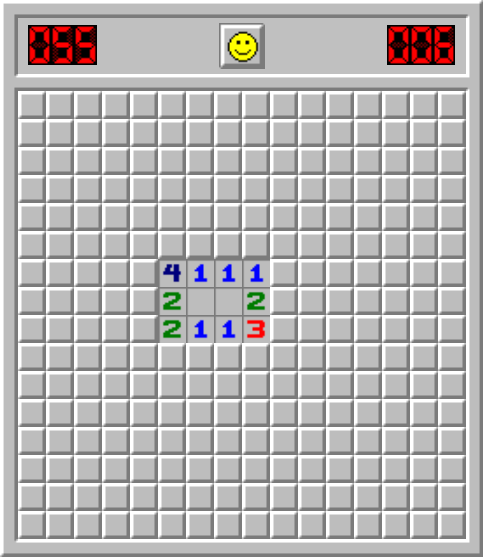
\includegraphics[width=5in]{images/MSProject4.png}
    \end{center}  
    \newpage
    \begin{center}
        Minesweeper Project Game 5\par\bigskip
		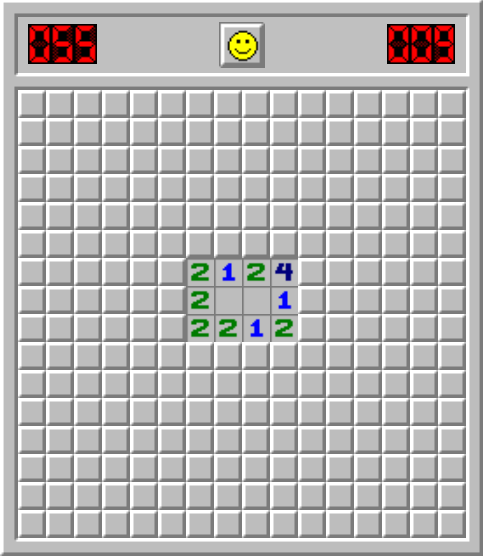
\includegraphics[width=5in]{images/MSProject5.png}
    \end{center}
    \newpage
    \begin{center}
        Minesweeper Project Game 6\par\bigskip
		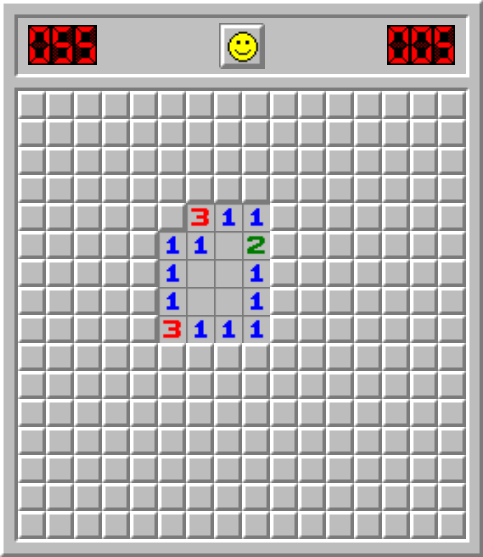
\includegraphics[width=5in]{images/MSProject6.png}
    \end{center}
    \newpage
    \begin{center}
        Minesweeper Project Game 7\par\bigskip
		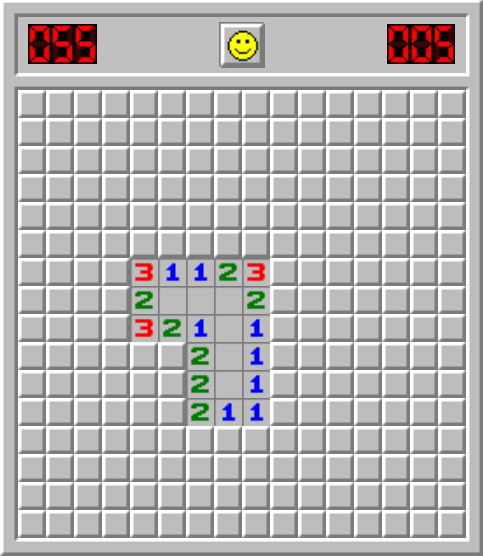
\includegraphics[width=5in]{images/MSProject7.png}
    \end{center}
    \newpage
    \begin{center}
        Minesweeper Project Game 8\par\bigskip
		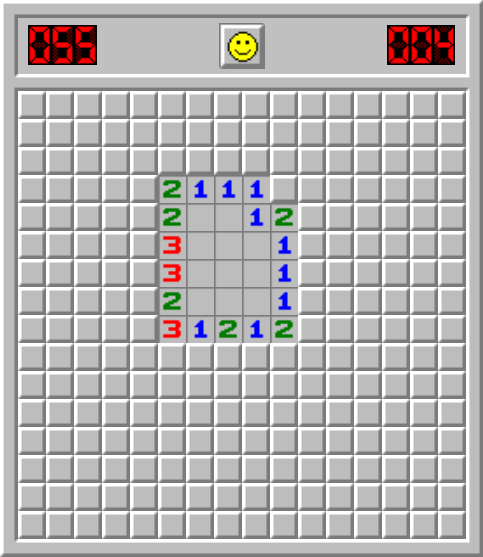
\includegraphics[width=5in]{images/MSProject8.png}
    \end{center}
    \newpage
    \begin{center}
        Minesweeper Project Game 9\par\bigskip
		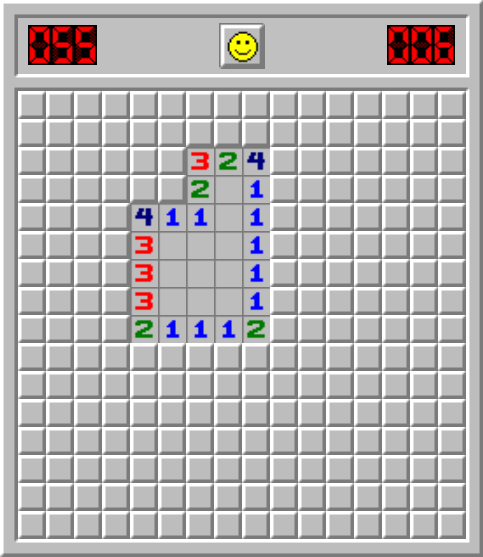
\includegraphics[width=5in]{images/MSProject9.png}
    \end{center}
    \newpage
    \begin{center}
        Minesweeper Project Game 10\par\bigskip
		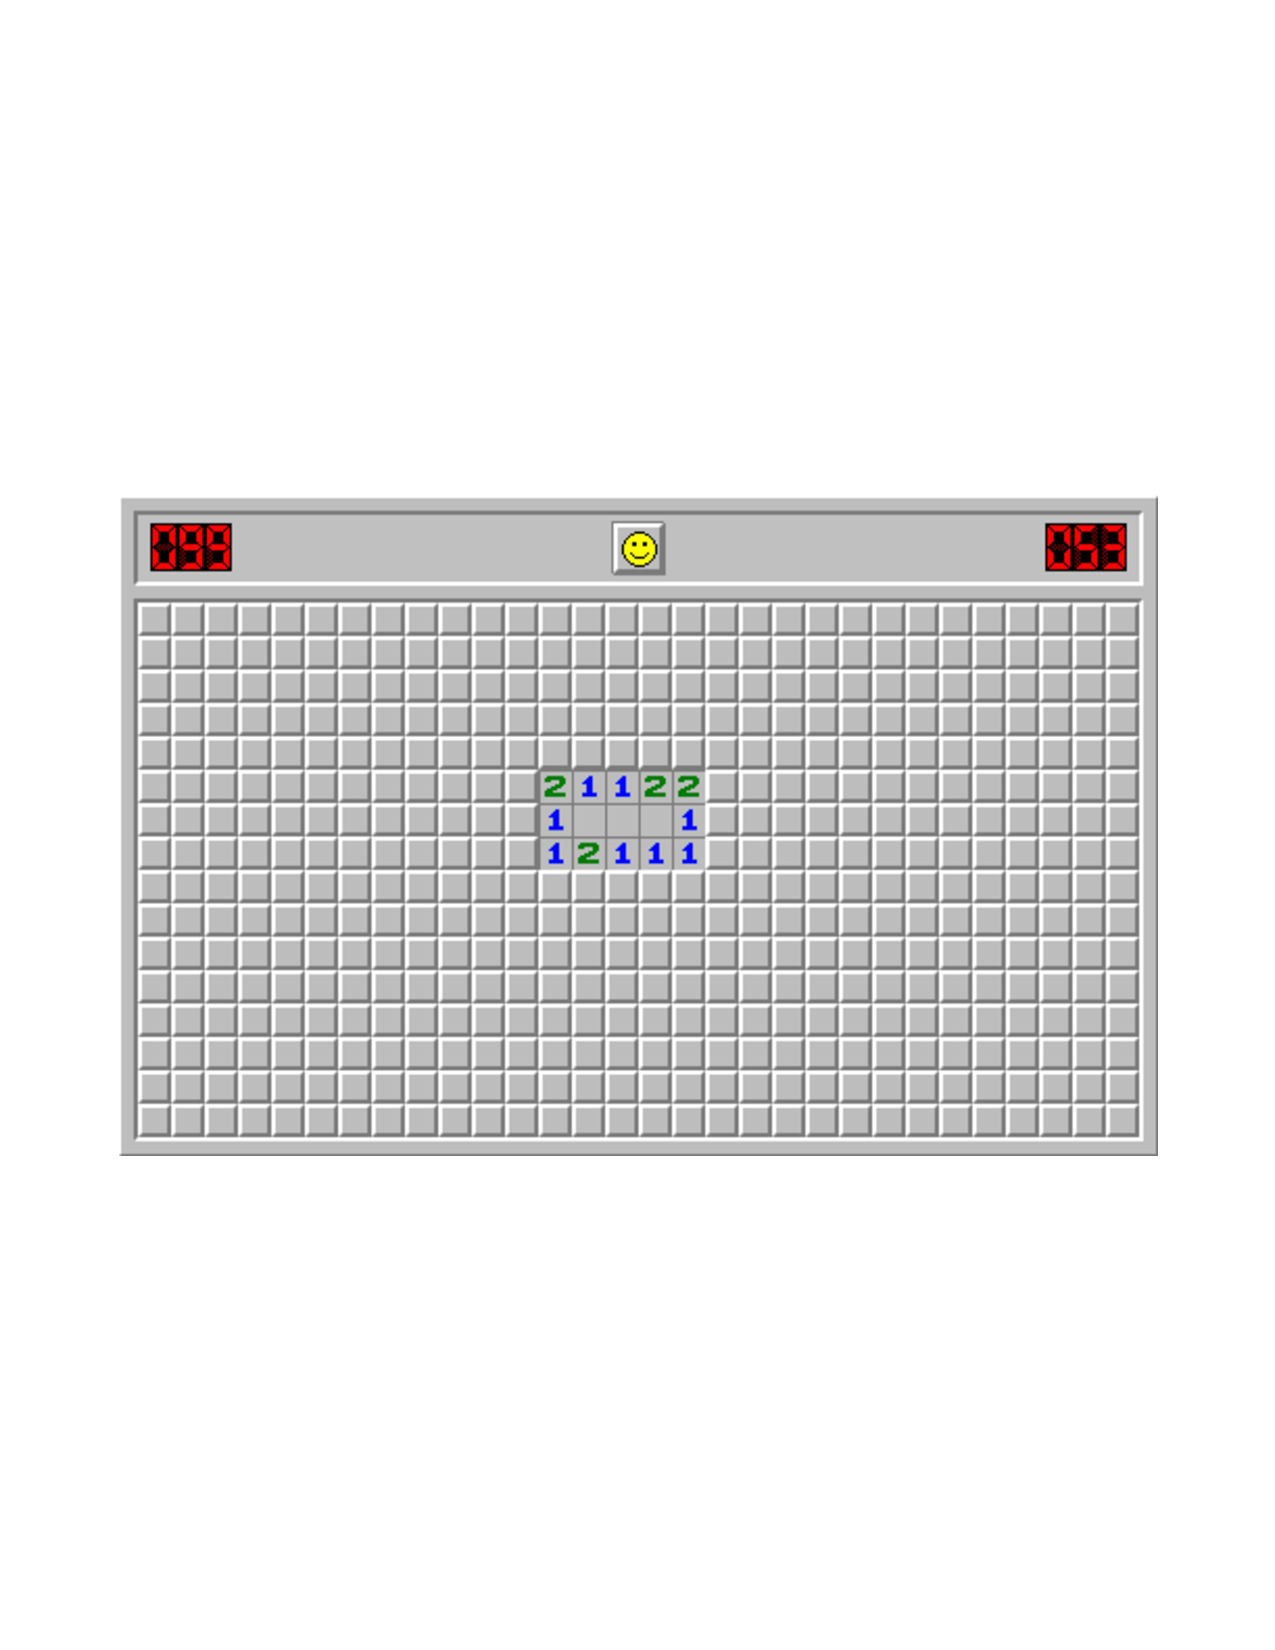
\includegraphics[width=6in]{images/MinesweeperSurrounded.pdf}
    \end{center}

    \newpage
    \begin{center}
        Nonogram Project Board 1\par\bigskip
        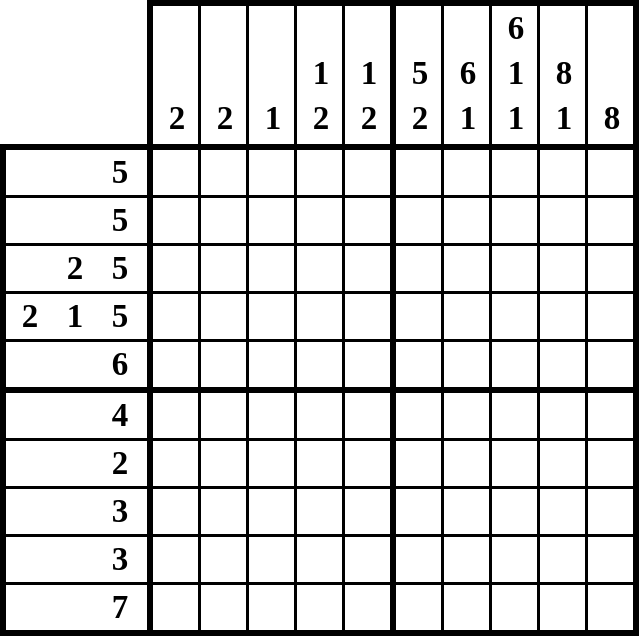
\includegraphics[width=5in]{images/nonogram01.png}
    \end{center}
    \newpage
    \begin{center}
        Nonogram Project Board 2\par\bigskip
        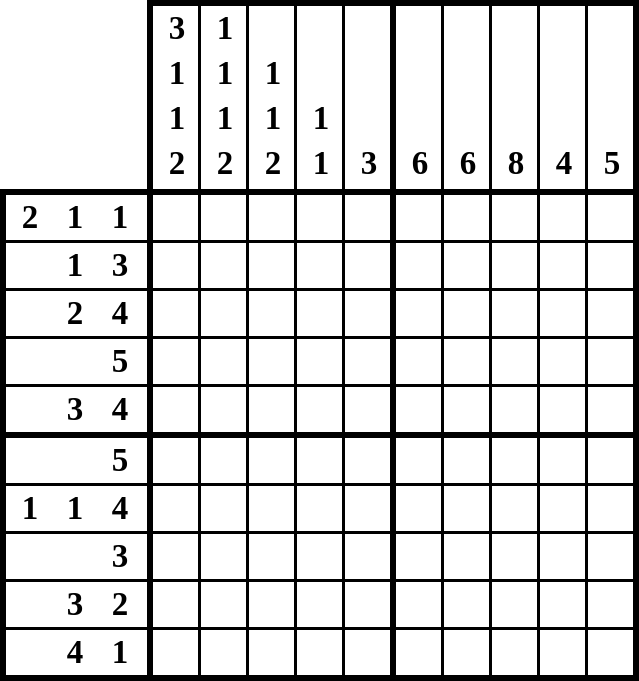
\includegraphics[width=5in]{images/nonogram02.png}
    \end{center}
    \newpage
    \begin{center}
        Nonogram Project Board 3\par\bigskip
        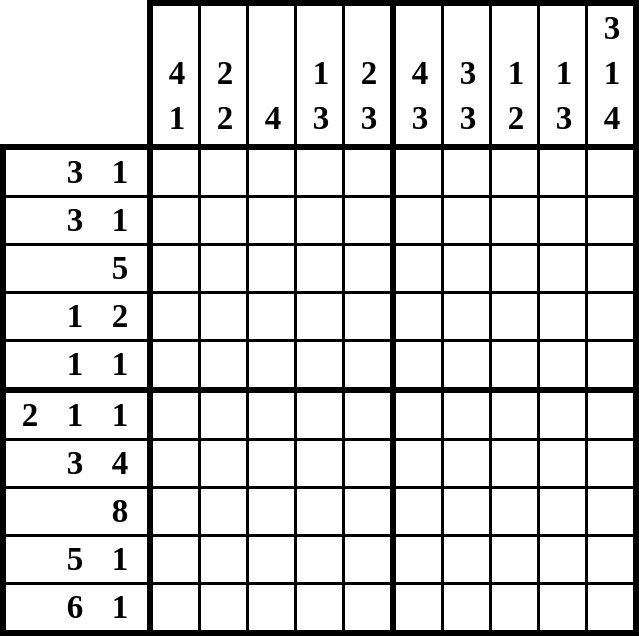
\includegraphics[width=5in]{images/nonogram03.png}
    \end{center}
    \newpage
    \begin{center}
        Nonogram Project Board 4\par\bigskip
        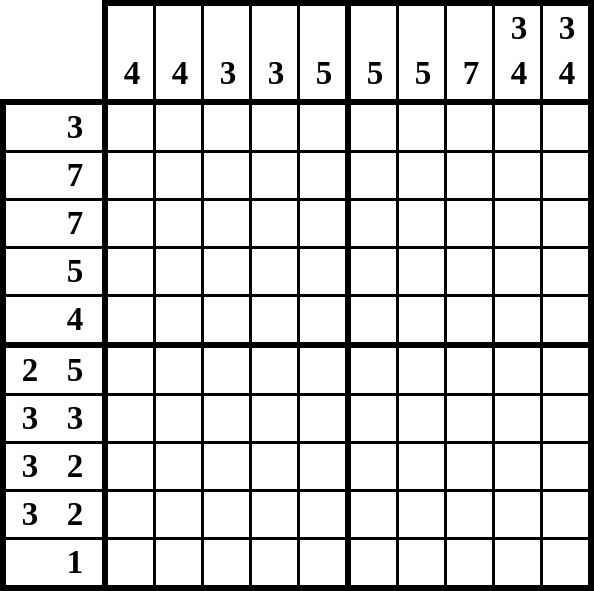
\includegraphics[width=5in]{images/nonogram04.png}
    \end{center}
    \newpage
    \begin{center}
        Nonogram Project Board 5\par\bigskip
        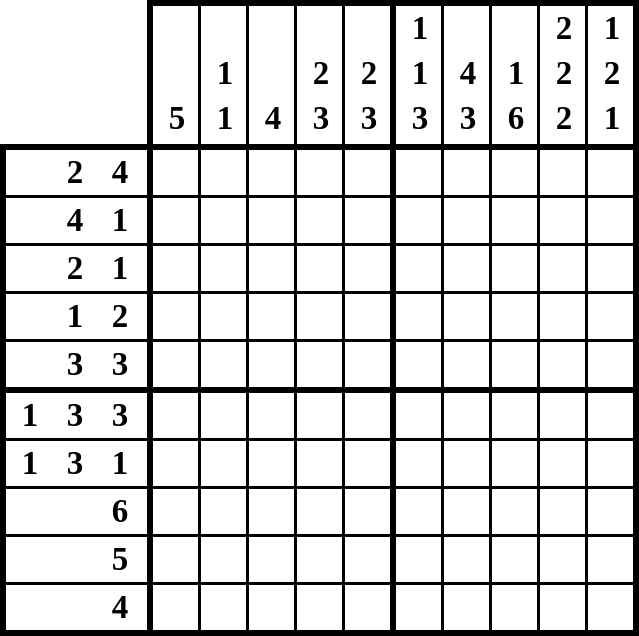
\includegraphics[width=5in]{images/nonogram05.png}
    \end{center}
    \newpage
    \begin{center}
        Nonogram Project Board 6\par\bigskip
        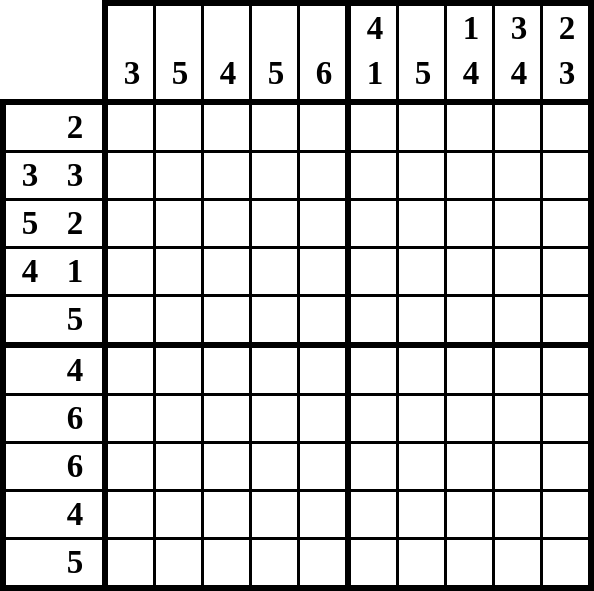
\includegraphics[width=5in]{images/nonogram06.png}
    \end{center}
    \newpage
    \begin{center}
        Nonogram Project Board 7\par\bigskip
        \includegraphics[width=5in]{images/nonogram07.png}
    \end{center}
    \newpage
    \begin{center}
        Nonogram Project Board 8\par\bigskip
        \includegraphics[width=5in]{images/nonogram08.png}
    \end{center}
    \newpage
    \begin{center}
        Nonogram Project Board 9\par\bigskip
        \includegraphics[width=5in]{images/nonogram09.png}
    \end{center}
    \newpage
    \begin{center}
        Nonogram Project Board 10\par\bigskip
        \includegraphics[width=5in]{images/nonogram10.png}
    \end{center}

    \newpage
    \begin{center}
        KenKen Project Puzzles 1\par\bigskip
        \includegraphics[width=2.8in]{images/kenken01a.png}\vfill
        \includegraphics[width=4.2in]{images/kenken01b.png}\vfill
    \end{center}
    \newpage
    \begin{center}
        KenKen Project Puzzles 2\par\bigskip
        \includegraphics[width=2.8in]{images/kenken02a.png}\vfill
        \includegraphics[width=4.2in]{images/kenken02b.png}\vfill
    \end{center}
    \newpage
    \begin{center}
        KenKen Project Puzzles 3\par\bigskip
        \includegraphics[width=2.8in]{images/kenken03a.png}\vfill
        \includegraphics[width=4.2in]{images/kenken03b.png}\vfill
    \end{center}
    \newpage
    \begin{center}
        KenKen Project Puzzles 4\par\bigskip
        \includegraphics[width=2.8in]{images/kenken04a.png}\vfill
        \includegraphics[width=4.2in]{images/kenken04b.png}\vfill
    \end{center}
    \newpage
    \begin{center}
        KenKen Project Puzzles 5\par\bigskip
        \includegraphics[width=2.8in]{images/kenken05a.png}\vfill
        \includegraphics[width=4.2in]{images/kenken05b.png}\vfill
    \end{center}
    \newpage
    \begin{center}
        KenKen Project Puzzles 6\par\bigskip
        \includegraphics[width=2.8in]{images/kenken06a.png}\vfill
        \includegraphics[width=4.2in]{images/kenken06b.png}\vfill
    \end{center}
    \newpage
    \begin{center}
        KenKen Project Puzzles 7\par\bigskip
        \includegraphics[width=2.8in]{images/kenken07a.png}\vfill
        \includegraphics[width=4.2in]{images/kenken07b.png}\vfill
    \end{center}
    \newpage
    \begin{center}
        KenKen Project Puzzles 8\par\bigskip
        \includegraphics[width=2.8in]{images/kenken08a.png}\vfill
        \includegraphics[width=4.2in]{images/kenken08b.png}\vfill
    \end{center}
    \newpage
    \begin{center}
        KenKen Project Puzzles 9\par\bigskip
        \includegraphics[width=2.8in]{images/kenken09a.png}\vfill
        \includegraphics[width=4.2in]{images/kenken09b.png}\vfill
    \end{center}
    \newpage
    \begin{center}
        KenKen Project Puzzles 10\par\bigskip
        \includegraphics[width=2.8in]{images/kenken10a.png}\vfill
        \includegraphics[width=4.2in]{images/kenken10b.png}\vfill
    \end{center}

\newpage
\begin{center}
        (2,5) - Sudoku Pair Puzzle 1
        
    \includegraphics[width=5in]{images/SPP1.png}
      \end{center}

\newpage
\begin{center}
        (2,5) - Sudoku Pair Puzzle Solution 1
        
    \includegraphics[width=5in]{images/SPP1Solved.png}
      \end{center}

\newpage
\begin{center}
        (2,5) - Sudoku Pair Puzzle 2
        
    \includegraphics[width=5in]{images/SPP2.png}
      \end{center}


\newpage
\begin{center}
        (2,5) - Sudoku Pair Puzzle 3
        
    \includegraphics[width=5in]{images/SPP3.png}
      \end{center}



\newpage
\begin{center}
        (2,5) - Sudoku Pair Puzzle 4
        
    \includegraphics[width=5in]{images/SPP4.png}
      \end{center}



\newpage
\begin{center}
        (2,5) - Sudoku Pair Puzzle 5
        
    \includegraphics[width=5in]{images/SPP5.png}
      \end{center}


\newpage
\begin{center}
        (2,5) - Sudoku Pair Puzzle 6
        
    \includegraphics[width=5in]{images/SPP6.png}
      \end{center}


\newpage
\begin{center}
        (2,5) - Sudoku Pair Puzzle 7
        
    \includegraphics[width=5in]{images/SPP7.png}
      \end{center}


\newpage
\begin{center}
        (2,5) - Sudoku Pair Puzzle 8
        
    \includegraphics[width=5in]{images/SPP8.png}
      \end{center}


\newpage
\begin{center}
        (2,5) - Sudoku Pair Puzzle 9
        
    \includegraphics[width=5in]{images/SPP9.png}
      \end{center}


\newpage
\begin{center}
        (2,5) - Sudoku Pair Puzzle 10
        
    \includegraphics[width=5in]{images/SPP10.png}
      \end{center}



\newpage
\begin{center}
        (2,5) - Sudoku Pair Puzzle Solution 1
        
    \includegraphics[width=5in]{images/SPP1Solved.png}
      \end{center}

\newpage
\begin{center}
        (2,5) - Sudoku Pair Puzzle Solution 2
        
    \includegraphics[width=5in]{images/SPP2Solved.png}
      \end{center}
    
\newpage
\begin{center}
        (2,5) - Sudoku Pair Puzzle Solution 3
        
    \includegraphics[width=5in]{images/SPP3Solved.png}
      \end{center}

\newpage
\begin{center}
        (2,5) - Sudoku Pair Puzzle Solution 4
        
    \includegraphics[width=5in]{images/SPP4Solved.png}
      \end{center}
\newpage

\newpage
\begin{center}
        (2,5) - Sudoku Pair Puzzle Solution 5
        
    \includegraphics[width=5in]{images/SPP5Solved.png}
      \end{center}

\newpage
\begin{center}
        (2,5) - Sudoku Pair Puzzle Solution 6
        
    \includegraphics[width=5in]{images/SPP6Solved.png}
      \end{center}
      
\newpage
\begin{center}
        (2,5) - Sudoku Pair Puzzle Solution 7
        
    \includegraphics[width=5in]{images/SPP7Solved.png}
      \end{center}

\newpage
\begin{center}
        (2,5) - Sudoku Pair Puzzle Solution 8
        
    \includegraphics[width=5in]{images/SPP8Solved.png}
      \end{center}


\newpage
\begin{center}
        (2,5) - Sudoku Pair Puzzle Solution 9
        
    \includegraphics[width=5in]{images/SPP9Solved.png}
      \end{center}

\newpage
\begin{center}
        (2,5) - Sudoku Pair Puzzle Solution 10
        
    \includegraphics[width=5in]{images/SPP10Solved.png}
      \end{center}
}

\newpage
%<*truthTables:exercises:title>
\section{Additional Exercises}
%</truthTables:exercises:title>

%<*truthTables:exercises:conTTableA>
\begin{enumerate}
\item Construct a truth table\index{truth table} for the following statements\index{statement}. \index{$\vee$}\index{$\wedge$}\index{$\neg$}\index{$\Rightarrow$}
\begin{enumerate}
\item $\neg(\neg P \wedge \neg Q)$
%</truthTables:exercises:conTTableA>

\Instr{ 
\begin{center}
\begin{tabular}{|c|c||c|}
\hline
$P$ & $Q$ & $\neg(\neg P\wedge \neg Q)$ \\
\hline
\hline
True & True & True \\
\hline
True & False & True \\
\hline
False & True & True \\
\hline
False & False & False \\
\hline
\end{tabular}
\end{center}
}

%<*truthTables:exercises:conTTableB>
\item $\neg(\neg P \vee \neg Q)$
%</truthTables:exercises:conTTableB>

\Instr{ 
\begin{center}
\begin{tabular}{|c|c||c|}
\hline
$P$ & $Q$ & $\neg(\neg P \vee \neg Q)$ \\
\hline
\hline
True & True & True \\
\hline
True & False & False \\
\hline
False & True & False \\
\hline
False & False & False \\
\hline
\end{tabular}
\end{center}
}

%<*truthTables:exercises:conTTableC>
\item $\neg(P\Rightarrow \neg Q)$
%</truthTables:exercises:conTTableC>

\Instr{ 

\begin{center}
\begin{tabular}{|c|c||c|}
\hline
$P$ & $Q$ & $\neg(P\Rightarrow \neg Q)$ \\
\hline
\hline
True & True & True \\
\hline
True & False & False \\
\hline
False & True & False \\
\hline
False & False & False \\
\hline
\end{tabular}
\end{center}
}

%<*truthTables:exercises:conTTableD>
\item $(P\vee Q)\Rightarrow P$
%</truthTables:exercises:conTTableD>

\Instr{ 
\begin{center}
\begin{tabular}{|c|c||c|}
\hline
$P$ & $Q$ & $(P\vee Q)\Rightarrow P$ \\
\hline
\hline
True & True & True \\
\hline
True & False & True \\
\hline
False & True & False \\
\hline
False & False & True \\
\hline
\end{tabular}
\end{center}
}

%<*truthTables:exercises:endifAndOnlyIf>
\end{enumerate}

\item\label{ifAndOnlyIf} The $\Leftrightarrow$ operator is known as the ``if and only if'' operator and is defined to be the statement $(P\Rightarrow Q)\wedge (Q\Rightarrow P)$. Its truth table is given in Table~{\normalfont\ref{iffTable}}. Find a way to write the statement $P\Leftrightarrow Q$\index{$\Leftrightarrow$} using the statements $P$ and $Q$, and the operators $\neg$, $\vee$, or $\wedge$. ({\em Hint}: Construct a truth table first.)

\begin{table}[H]
\begin{center}
\begin{tabular}{|c|c||c|}
\hline
$P$ & $Q$ & $P\Leftrightarrow Q$ \\
\hline
\hline
True & True & True \\
\hline
True & False & False \\
\hline
False & True & False \\
\hline
False & False & True \\
\hline
\end{tabular}
\end{center}
\caption{Truth table for $\Leftrightarrow$ operator}\label{iffTable}
\end{table}
%</truthTables:exercises:endifAndOnlyIf>

\Instr{  By constructing a truth table, it is easy to see $(P\wedge Q)\vee(\neg P\wedge \neg Q)$ is equivalent to $P\Leftrightarrow Q$.
}

%<*truthTables:exercises:conMoreTTableA>
\item Construct a truth table for the following statements\index{statement}\index{$\neg$}\index{$\wedge$}\index{$\vee$}\index{$\Rightarrow$}\index{$\Leftrightarrow$}.
\begin{enumerate}
\item $\neg P\Leftrightarrow P$
%</truthTables:exercises:conMoreTTableA>

\Instr{ 
\begin{center}
\begin{tabular}{|c|c||c|}
\hline
$P$ & $Q$ & $\neg P \Leftrightarrow P$ \\
\hline
\hline
True & True & False \\
\hline
True & False & False \\
\hline
False & True & False \\
\hline
False & False & False \\
\hline
\end{tabular}
\end{center}
}

%<*truthTables:exercises:conMoreTTableB>
\item $\neg (P\vee Q) \Leftrightarrow (\neg P\wedge \neg Q)$ 
%</truthTables:exercises:conMoreTTableB>

\Instr{ 
\begin{center}
\begin{tabular}{|c|c||c|}
\hline
$P$ & $Q$ & $\neg (P\vee Q) \Leftrightarrow (\neg P\wedge \neg Q)$ \\
\hline
\hline
True & True & True \\
\hline
True & False & True \\
\hline
False & True & True \\
\hline
False & False & True \\
\hline
\end{tabular}
\end{center}
}

%<*truthTables:exercises:conMoreTTableC>
\item $\neg(P\Rightarrow Q)\Rightarrow (\neg Q\Rightarrow P)$
%</truthTables:exercises:conMoreTTableC>

\Instr{ 
\begin{center}
\begin{tabular}{|c|c||c|}
\hline
$P$ & $Q$ & $\neg(P\Rightarrow Q)\Rightarrow (\neg Q\Rightarrow P)$ \\
\hline
\hline
True & True & True \\
\hline
True & False & True \\
\hline
False & True & True \\
\hline
False & False & True \\
\hline
\end{tabular}
\end{center}
}

%<*truthTables:exercises:conMoreTTableD>
\item $((P\Leftrightarrow Q)\wedge (P\Rightarrow R))\vee (\neg P\Rightarrow (Q\wedge R))$
%</truthTables:exercises:conMoreTTableD>

\Instr{ 
\begin{center}
\begin{tabular}{|c|c|c||c|}
\hline
$P$ & $Q$ & $R$ & $((P\Leftrightarrow Q)\wedge (P\Rightarrow R))\vee (\neg P\Rightarrow (Q\wedge R))$ \\
\hline
\hline
True & True & True & True \\
\hline
True & True & False & True \\
\hline
True & False & True & True \\
\hline
True & False & False & True \\
\hline
False & True & True & True \\
\hline
False & True & False & False \\
\hline
False & False & True & True \\
\hline
False & False & False & True \\
\hline
\end{tabular}
\end{center}
}

%<*truthTables:exercises:conMoreTTableE>
\item $\neg (\neg P\Rightarrow (Q\vee R))\Rightarrow (\neg P \wedge Q)$
%</truthTables:exercises:conMoreTTableE>

\Instr{ 
\begin{center}
\begin{tabular}{|c|c|c||c|}
\hline
$P$ & $Q$ & $R$ & $\neg (\neg P\Rightarrow (Q\vee R))\Rightarrow (\neg P \wedge Q)$ \\
\hline
\hline
True & True & True & True \\
\hline
True & True & False & True \\
\hline
True & False & True & True \\
\hline
True & False & False & True \\
\hline
False & True & True & True \\
\hline
False & True & False & True \\
\hline
False & False & True & False \\
\hline
False & False & False & False \\
\hline
\end{tabular}
\end{center}
}
%<*truthTables:exercises:endTautology>
\end{enumerate}

\item Write a single statement using $P$, $Q$, and $R$ along with the symbols $\neg$, $\vee$, $\wedge$, or $\Rightarrow$ that is always true.
%</truthTables:exercises:endTautology>

\Instr{  
There are many solutions to this question. One such statement is $((P\vee Q)\vee R)\vee \neg P$. Any statement that is always true is called a \textbf{tautology}\index{tautology}.
}

%<*truthTables:exercises:stateJake>
\item Consider the following statements about Jake. 

\begin{minipage}[H]{5.75in}
\tt
\begin{center}
{ ``If today is Wednesday, then Jake's class has library day. If Jake's class has library day, then Jake will bring home a new book. Jake did not bring any new books home today.''}
\end{center}
\end{minipage}

What can you conclude based on the given information? Explain your answer.
%</truthTables:exercises:stateJake>

\Instr{  Since Jake did not bring a book home we can assume that Jake's class did not have library day. Also, since Jake's class did not have library day, you may conclude that today must not be Wednesday. 

This can be explained in a different way using statements as well. Let the statement ``today is Wednesday'' be $P$, the statement ``Jake's class has library day'' be $Q$, and the statement ``Jake will bring home a new book'' be $R$. Then the first sentence says $P\Rightarrow Q$, the second sentence says $Q\Rightarrow R$ and the last sentence says $R$ is false. For the statement $Q\Rightarrow R$ to hold true, $Q$ must be false and so Jake's class did not have library day. Similarly, For the statement $P\Rightarrow Q$ to hold true, $P$ must be false, so today is not Wednesday.
}

%<*truthTables:exercises:equalState>
\item Show that the two statements\index{statement} $((P\wedge Q)\Rightarrow R)$\index{$\wedge$}\index{$\Rightarrow$}\index{$\neg$}\index{$\vee$} and $(\neg P)\vee (\neg Q) \vee R$ are equivalent. Give an example in which $P$, $Q$, and $R$ each stand for some statement (like in Activity~{\normalfont\ref{conditional}}, then explain what the statements $((P\wedge Q)\Rightarrow R)$ and $(\neg P)\vee (\neg Q) \vee R$ mean in your given context.
%</truthTables:exercises:equalState>

\Instr{  The following truth table shows that the statements $((P\wedge Q)\Rightarrow R)$ and $(\neg P)\vee(\neg Q)\vee R$ are equivalent.
\begin{center}
\begin{tabular}{|c|c|c||c|c|}
\hline
$P$ & $Q$ & $R$ & $((P\wedge Q)\Rightarrow R)$ & $(\neg P)\vee (\neg Q)\vee R$ \\
\hline
\hline
True & True & True & True & True \\
\hline
True & True & False & False & False \\
\hline
True & False & True & True & True \\
\hline
True & False & False & True & True \\
\hline
False & True & True & True & True \\
\hline
False & True & False & True & True \\
\hline
False & False & True & True & True \\
\hline
False & False & False & True & True \\
\hline
\end{tabular}
\end{center}

Let statement $P$ be ``I drive to work'', statement $Q$ be ``I wear brown pants'', and statement $R$ be ``I wear brown shoes.'' Then $((P\wedge Q)\Rightarrow R)$ says if I drive to work and wear brown pants, then I will wear brown shoes. The statement $(\neg P)\vee (\neg Q)\vee R$ says I will not drive to work or I will not wear brown pants or I will wear brown shoes.
}

%<*truthTables:exercises:matchTTablePreA>
\item Write out a statement\index{statement} using $P$ and $Q$ with the operators $\neg$, $\wedge$, or $\vee$ that has the indicated truth table\index{truth table}.
%</truthTables:exercises:matchTTablePreA>

\Instr{  Each question has multiple solutions. We give one possible answer.
}

%<*truthTables:exercises:matchTTableA>
\begin{enumerate}
\item \mbox{}
\begin{center}
\begin{tabular}{|c|c||c|}
\hline
$P$ & $Q$ & \hspace{1.75in} \\
\hline
\hline
True & True & True \\
\hline
True & False & True \\
\hline
False & True & False \\
\hline
False & False & True \\
\hline
\end{tabular}
\end{center}
%</truthTables:exercises:matchTTableA>

\Instr{  
\begin{center}
\begin{tabular}{|c|c||c|}
\hline
$P$ & $Q$ & $\neg Q\vee P$ \\
\hline
\hline
True & True & True \\
\hline
True & False & True \\
\hline
False & True & False \\
\hline
False & False & True \\
\hline
\end{tabular}
\end{center}
}

%<*truthTables:exercises:matchTTableB>
\item \mbox{}
\begin{center}
\begin{tabular}{|c|c||c|}
\hline
$P$ & $Q$ & \hspace{1.75in} \\
\hline
\hline
True & True & False \\
\hline
True & False & False \\
\hline
False & True & True \\
\hline
False & False & False \\
\hline
\end{tabular}
\end{center}
%</truthTables:exercises:matchTTableB>

\Instr{ 
\begin{center}
\begin{tabular}{|c|c||c|}
\hline
$P$ & $Q$ & $\neg(\neg Q\vee P)=Q\wedge \neg P$ \\
\hline
\hline
True & True & False \\
\hline
True & False & False \\
\hline
False & True & True \\
\hline
False & False & False \\
\hline
\end{tabular}
\end{center}
}

%<*truthTables:exercises:matchTTableC>
\item \mbox{}
\begin{center}
\begin{tabular}{|c|c||c|}
\hline
$P$ & $Q$ & \hspace{1.75in} \\
\hline
\hline
True & True & True \\
\hline
True & False & True \\
\hline
False & True & True \\
\hline
False & False & True \\
\hline
\end{tabular}
\end{center}
%</truthTables:exercises:matchTTableC>

\Instr{  
\begin{center}
\begin{tabular}{|c|c||c|}
\hline
$P$ & $Q$ & $(P\vee Q)\vee \neg P$ \\
\hline
\hline
True & True & True \\
\hline
True & False & True \\
\hline
False & True & True \\
\hline
False & False & True \\
\hline
\end{tabular}
\end{center}
}

%<*truthTables:exercises:matchTTableD>
\item \mbox{}
\begin{center}
\begin{tabular}{|c|c||c|}
\hline
$P$ & $Q$ & \hspace{1.75in} \\
\hline
\hline
True & True & True \\
\hline
True & False & True \\
\hline
False & True & True \\
\hline
False & False & False \\
\hline
\end{tabular}
\end{center}
%</truthTables:exercises:matchTTableD>

\Instr{  
\begin{center}
\begin{tabular}{|c|c||c|}
\hline
$P$ & $Q$ & $P\vee Q$ \\
\hline
\hline
True & True & True \\
\hline
True & False & True \\
\hline
False & True & True \\
\hline
False & False & False \\
\hline
\end{tabular}
\end{center}
}

%<*truthTables:exercises:matchTTableE>
\item \mbox{}
\begin{center}
\begin{tabular}{|c|c||c|}
\hline
$P$ & $Q$ & \hspace{1.75in} \\
\hline
\hline
True & True & False \\
\hline
True & False & False \\
\hline
False & True & True \\
\hline
False & False & True \\
\hline
\end{tabular}
\end{center}
%</truthTables:exercises:matchTTableE>

\Instr{ 
\begin{center}
\begin{tabular}{|c|c||c|}
\hline
$P$ & $Q$ & $\neg P$ or $\neg P \wedge (\neg P\vee \neg Q)$ \\
\hline
\hline
True & True & False \\
\hline
True & False & False \\
\hline
False & True & True \\
\hline
False & False & True \\
\hline
\end{tabular}
\end{center}
}
%<*truthTables:exercises:endOplus>
\end{enumerate}

\item The $\oplus$ symbol is known as XOR and is the statement that is true if exactly one of $P$ and $Q$ is true. Its truth table is given in Table~{\normalfont\ref{xorTable}}. Write a statement that is equivalent to $P\oplus Q$\index{$\oplus$} using the symbols $\neg$, $\vee$, or $\wedge$. 

\begin{table}[H]
\begin{center}
\begin{tabular}{|c|c||c|}
\hline
$P$ & $Q$ & $P\oplus Q$ \\
\hline
\hline
True & True & False \\
\hline
True & False & True \\
\hline
False & True & True \\
\hline
False & False & False \\
\hline
\end{tabular}
\end{center}
\caption{Truth table for $\oplus$ symbol}\label{xorTable}
\end{table}
%</truthTables:exercises:endOplus>

\Instr{  By constructing a truth table, it is easy to see $(P\vee Q)\wedge \neg(P\wedge Q)$ is equivalent to $P\oplus Q$. There are other solutions as well.
}

%<*truthTables:exercises:stateMoreEqualA>
\item Show that the pair of statements\index{statement} are equivalent using truth tables\index{truth table}.
\begin{enumerate}
\item $\neg (P \wedge Q)$ and $\neg P \vee \neg Q$
%</truthTables:exercises:stateMoreEqualA>

\Instr{  
\begin{center}
\begin{tabular}{|c|c||c|c|}
\hline
$P$ & $Q$ & $\neg(P\wedge Q)$ & $\neg P \vee \neg Q$ \\
\hline
\hline
True & True & False & False \\
\hline
True & False & True & True \\
\hline
False & True & True & True \\
\hline
False & False & True & True \\
\hline
\end{tabular}
\end{center}
}

%<*truthTables:exercises:stateMoreEqualB>
\item $((P\vee Q)\wedge (\neg P)) \wedge Q$ and $\neg P\wedge Q$\index{$\wedge$}\index{$\vee$}\index{$\neg$}
%</truthTables:exercises:stateMoreEqualB>

\Instr{ 
\begin{center}
\begin{tabular}{|c|c||c|c|}
\hline
$P$ & $Q$ & $((P\vee Q)\wedge(\neg P))\wedge Q$ & $\neg P\wedge Q$ \\
\hline
\hline
True & True & False & False \\
\hline
True & False & False & False \\
\hline
False & True & True & True \\
\hline
False & False & False & False \\
\hline
\end{tabular}
\end{center}
}
%<*truthTables:exercises:endTrueLie>
\end{enumerate}

\item\label{trueLie} During your voyage across the $7$ seas you come across an island that is populated by two tribes: monks and peasants (or so they call themselves). From your interaction with them you realize that the monks always tell the truth while the peasants tell nothing but lies. Unfortunately, you cannot tell the inhabitants apart from each other. One day, two of the inhabitants, let us call them Amber and Betty, came up to you to tell you something:
\begin{itemize}
\item[] Amber says ``Exactly one of us is a monk.''
\item[] Betty says ``Only a peasant would say that Amber is a peasant.''
\end{itemize}
Can you determine to which tribe each of Amber and Betty belong?
%</truthTables:exercises:endTrueLie>

\Instr{ 
Let $A$ represent the statement made by Amber and $B$ represent the statement made by Betty. 

Suppose $A$ is true. Then either Amber or Betty is a monk but not both. Since $A$ is true, it follows that Amber is a monk, and so make Betty the peasant. Before we jump to any conclusions and declare a solution, we need to make sure Betty's statement makes sense knowing that her statement is false. Since $B$ is false, it is not true that a peasant would say that Amber is a peasant, but this is a contradiction. 

Suppose $A$ is false. Then Amber is a peasant and it is not true that either Amber or Betty is a monk but not both. So either Amber and Betty are both peasants or are both monks. Since Amber is a peasant, Betty is peasant. Finally, we must check that it makes sense that $B$ is false. Since $B$ is false, it is not true that a peasant would say that Amber is a peasant. Since Amber is a peasant it would make sense that statement $B$ is false. So both Amber and Betty are both peasants.
}

%<*truthTables:exercises:anotherTrueLie>
\item You meet another inhabitant of island described in Question~{\normalfont\ref{trueLie}}. You ask an inhabitant if there is gold on the island. He tells you ``There is gold on this island if and only if I am a monk.'' Translate this statement\index{statement} into a logical symbol. Is this person a monk or peasant? Is there gold on the island. ({\em Hint}: The ``if and only if'' operator ($\Leftrightarrow$) is discussed in Question~{\normalfont\ref{ifAndOnlyIf}}.)
%</truthTables:exercises:anotherTrueLie>

\Instr{ 
Let $P$ be the statement that there is gold on this island and let $Q$ be the statement be I am a monk. So the logical statement made in the question is $P\Leftrightarrow Q$. 

Suppose the inhabitant is a peasant. Then $Q$ and the logical statement $P\Leftrightarrow Q$ are false. By examining the table in Question~{\normalfont\ref{ifAndOnlyIf}} we see that the only way this would hold is if $P$ is true. So there would be gold on the island. No contradictions were made at this time so we must see what happens when we assume that the inhabitant is a monk. 

Suppose this inhabitant is a monk. Then $Q$ and the logical statement $P\Leftrightarrow Q$ are true. By looking back at the table in Question~{\normalfont\ref{ifAndOnlyIf}} the only way $Q$ and the statement $P\Leftrightarrow Q$ are true is if $P$ is true. So there is gold on this island. Again, no breaks in logic were made. We may never know if the inhabitant is a monk or peasant, but we know for certain that there must be gold on the island.
}

%<*truthTables:exercises:newSymbol>
\item Construct a new symbol $*$ that gives true or false responses depending on whether the statements are true or false (just like $\vee$, $\wedge$, and $\Rightarrow$). Explain how it works. Fill in the first three columns of the following table to make it clear what $P*Q$ means. Then fill in the remainder of the truth table\index{truth table}.

\begin{center}
\begin{tabular}{|c|c||c|c|c|c|c||}
\hline
$P$ & $Q$ & $P*Q$ & $((P * Q)\wedge P)\Rightarrow Q$ & $((P\Rightarrow \neg Q) *Q)\Rightarrow \neg P$ & $P*Q \Rightarrow P$  \\
\hline
\hline
\hspace{.4in} & \hspace{.4in} & \hspace{.4in} & \hspace{.4in} &  & \\
\hline
&&&&& \\
\hline
&&&&& \\
\hline
&&&&& \\
\hline
\end{tabular}
\end{center}
%</truthTables:exercises:newSymbol>

\Instr{ 
The answer to this question are dependent on what $P*Q$ means to each student. There are $2^4=16$ different ways the third column can be filled in and to this end, we provide all possible solutions below. 
\begin{center}
\begin{tabular}{|c|c||c|c|c|c|c||}
\hline
$P$ & $Q$ & $P*Q$ & $((P * Q)\wedge P)\Rightarrow Q$ & $((P\Rightarrow \neg Q) *Q)\Rightarrow \neg P$ & $P*Q \Rightarrow P$  \\
\hline
\hline
True & True & True & True & False & True \\
\hline
True & False & True & False & False & False \\
\hline
False & True & True & True & True & True \\
\hline
False & False & True & True & True & False \\
\hline
\end{tabular}
\end{center}
\begin{center}
\begin{tabular}{|c|c||c|c|c|c|c||}
\hline
$P$ & $Q$ & $P*Q$ & $((P * Q)\wedge P)\Rightarrow Q$ & $((P\Rightarrow \neg Q) *Q)\Rightarrow \neg P$ & $P*Q \Rightarrow P$  \\
\hline
\hline
True & True & True & True & False & True \\
\hline
True & False & True & False & False & False \\
\hline
False & True & True & True & True & True\\
\hline
False & False & False & True & True & True \\
\hline
\end{tabular}
\end{center}
\begin{center}
\begin{tabular}{|c|c||c|c|c|c|c||}
\hline
$P$ & $Q$ & $P*Q$ & $((P * Q)\wedge P)\Rightarrow Q$ & $((P\Rightarrow \neg Q) *Q)\Rightarrow \neg P$ & $P*Q \Rightarrow P$  \\
\hline
\hline
True & True & True & True & True & True \\
\hline
True & False & True & False & False & False \\
\hline
False & True & False & True & True & True \\
\hline
False & False & True & True & True & False \\
\hline
\end{tabular}
\end{center}
\begin{center}
\begin{tabular}{|c|c||c|c|c|c|c||}
\hline
$P$ & $Q$ & $P*Q$ & $((P * Q)\wedge P)\Rightarrow Q$ & $((P\Rightarrow \neg Q) *Q)\Rightarrow \neg P$ & $P*Q \Rightarrow P$  \\
\hline
\hline
True & True & True & True & True & True \\
\hline
True & False & True & False & False & False \\
\hline
False & True & False & True & True & True \\
\hline
False & False & False & True & True & True \\
\hline
\end{tabular}
\end{center}
\begin{center}
\begin{tabular}{|c|c||c|c|c|c|c||}
\hline
$P$ & $Q$ & $P*Q$ & $((P * Q)\wedge P)\Rightarrow Q$ & $((P\Rightarrow \neg Q) *Q)\Rightarrow \neg P$ & $P*Q \Rightarrow P$  \\
\hline
\hline
True & True & True & True & False & True \\
\hline
True & False & False & True & True & True \\
\hline
False & True & True & True & True & True \\
\hline
False & False & True & True & True & False \\
\hline
\end{tabular}
\end{center}
\begin{center}
\begin{tabular}{|c|c||c|c|c|c|c||}
\hline
$P$ & $Q$ & $P*Q$ & $((P * Q)\wedge P)\Rightarrow Q$ & $((P\Rightarrow \neg Q) *Q)\Rightarrow \neg P$ & $P*Q \Rightarrow P$  \\
\hline
\hline
True & True & True & True & False & True \\
\hline
True & False & False & True & True & True \\
\hline
False & True & True & True & True & True \\
\hline
False & False & False & True & True & True \\
\hline
\end{tabular}
\end{center}
\begin{center}
\begin{tabular}{|c|c||c|c|c|c|c||}
\hline
$P$ & $Q$ & $P*Q$ & $((P * Q)\wedge P)\Rightarrow Q$ & $((P\Rightarrow \neg Q) *Q)\Rightarrow \neg P$ & $P*Q \Rightarrow P$  \\
\hline
\hline
True & True & True & True & True & True \\
\hline
True & False & False & True & True & True \\
\hline
False & True & False & True & True & True \\
\hline
False & False & True & True & True & False \\
\hline
\end{tabular}
\end{center}
\begin{center}
\begin{tabular}{|c|c||c|c|c|c|c||}
\hline
$P$ & $Q$ & $P*Q$ & $((P * Q)\wedge P)\Rightarrow Q$ & $((P\Rightarrow \neg Q) *Q)\Rightarrow \neg P$ & $P*Q \Rightarrow P$  \\
\hline
\hline
True & True & True & True & True & True \\
\hline
True & False & False & True & True & True \\
\hline
False & True & False & True & True & True \\
\hline
False & False & False & True & True & True \\
\hline
\end{tabular}
\end{center}
\begin{center}
\begin{tabular}{|c|c||c|c|c|c|c||}
\hline
$P$ & $Q$ & $P*Q$ & $((P * Q)\wedge P)\Rightarrow Q$ & $((P\Rightarrow \neg Q) *Q)\Rightarrow \neg P$ & $P*Q \Rightarrow P$  \\
\hline
\hline
True & True & False & True & False & True \\
\hline
True & False & True & False & False & False \\
\hline
False & True & True & True & True & True \\
\hline
False & False & True & True & True & False \\
\hline
\end{tabular}
\end{center}
\begin{center}
\begin{tabular}{|c|c||c|c|c|c|c||}
\hline
$P$ & $Q$ & $P*Q$ & $((P * Q)\wedge P)\Rightarrow Q$ & $((P\Rightarrow \neg Q) *Q)\Rightarrow \neg P$ & $P*Q \Rightarrow P$  \\
\hline
\hline
True & True & False & True & False & True \\
\hline
True & False & True & False & False & False \\
\hline
False & True & True & True & True & True \\
\hline
False & False & False & True & True & True \\
\hline
\end{tabular}
\end{center}
\begin{center}
\begin{tabular}{|c|c||c|c|c|c|c||}
\hline
$P$ & $Q$ & $P*Q$ & $((P * Q)\wedge P)\Rightarrow Q$ & $((P\Rightarrow \neg Q) *Q)\Rightarrow \neg P$ & $P*Q \Rightarrow P$  \\
\hline
\hline
True & True & False & True & True & True \\
\hline
True & False & True & False & False & False \\
\hline
False & True & False & True & True & True \\
\hline
False & False & True & True & True & False \\
\hline
\end{tabular}
\end{center}
\begin{center}
\begin{tabular}{|c|c||c|c|c|c|c||}
\hline
$P$ & $Q$ & $P*Q$ & $((P * Q)\wedge P)\Rightarrow Q$ & $((P\Rightarrow \neg Q) *Q)\Rightarrow \neg P$ & $P*Q \Rightarrow P$  \\
\hline
\hline
True & True & False & True & True & True \\
\hline
True & False & True & False & False & False \\
\hline
False & True & False & True & True & True \\
\hline
False & False & False & True & True & True \\
\hline
\end{tabular}
\end{center}
\begin{center}
\begin{tabular}{|c|c||c|c|c|c|c||}
\hline
$P$ & $Q$ & $P*Q$ & $((P * Q)\wedge P)\Rightarrow Q$ & $((P\Rightarrow \neg Q) *Q)\Rightarrow \neg P$ & $P*Q \Rightarrow P$  \\
\hline
\hline
True & True & False & True & False & True \\
\hline
True & False & False & True & True & True \\
\hline
False & True & True & True & True & True \\
\hline
False & False & True & True & True & False \\
\hline
\end{tabular}
\end{center}
\begin{center}
\begin{tabular}{|c|c||c|c|c|c|c||}
\hline
$P$ & $Q$ & $P*Q$ & $((P * Q)\wedge P)\Rightarrow Q$ & $((P\Rightarrow \neg Q) *Q)\Rightarrow \neg P$ & $P*Q \Rightarrow P$  \\
\hline
\hline
True & True & False & True & False & True \\
\hline
True & False & False & True & True & True \\
\hline
False & True & True & True & True & True \\
\hline
False & False & False & True & True & True \\
\hline
\end{tabular}
\end{center}
\begin{center}
\begin{tabular}{|c|c||c|c|c|c|c||}
\hline
$P$ & $Q$ & $P*Q$ & $((P * Q)\wedge P)\Rightarrow Q$ & $((P\Rightarrow \neg Q) *Q)\Rightarrow \neg P$ & $P*Q \Rightarrow P$  \\
\hline
\hline
True & True & False & True & True & True \\
\hline
True & False & False & True & True & True \\
\hline
False & True & False & True & True & True \\
\hline
False & False & True & True & True & False \\
\hline
\end{tabular}
\end{center}
\begin{center}
\begin{tabular}{|c|c||c|c|c|c|c||}
\hline
$P$ & $Q$ & $P*Q$ & $((P * Q)\wedge P)\Rightarrow Q$ & $((P\Rightarrow \neg Q) *Q)\Rightarrow \neg P$ & $P*Q \Rightarrow P$  \\
\hline
\hline
True & True & False & True & True & True \\
\hline
True & False & False & True & True & True \\
\hline
False & True & False & True & True & True \\
\hline
False & False & False & True & True & True \\
\hline
\end{tabular}
\end{center}
}


%<*truthTables:exercises:end>
\end{enumerate}
%</truthTables:exercises:end>


% New Chapter %%%%%%%%%%%%%%%%%%%%%%%%%%%%%%%%%%%%%%%%%%%%%%%%
%
\chapter{Proportions, Ratios, and Scaling}\label{chap:proportions}
%
%%%%%%%%%%%%%%%%%%%%%%%%%%%%%%%%%%%%%%%%%%%%%%%%%%%%%%%%%%%%%%

\setcounter{section}{-1}
% New Section %%%%%%%%%%%%%%%%%%%%%%%%%%%%%%%%%%%%%%%%%%%%%%%%
\section{Mathematical Outcome}\label{sec:RatiosOutcome}
%%%%%%%%%%%%%%%%%%%%%%%%%%%%%%%%%%%%%%%%%%%%%%%%%%%%%%%%%%%%%%
The activities of this section are designed to strengthen understanding of fractions and the related concepts of ratios and similarity through applications of proportion, ratio, and scaling. For unit conversion it is assumed the student has a working knowledge of fractions including multiplication and division thereof. The sections on ratios and similarity are presented assuming little to no prior knowledge of the topics.

Through a series of activities mostly focused on things in the world around us such as the moon, peoples' eyes, and the buildings in which we teach and learn, students will
\begin{enumerate}
\item learn to convert units through multiplying fractions
\item work with ratios
\item see the connection between equivalent fractions and equivalent ratios
\item connect proportionality and scale with the world around them
\item calculate heights and weights of large objects by gathering data about smaller ones and using mathematics to extrapolate
\item explore the concept of self-similarity
\end{enumerate}

\newpage
% New Section %%%%%%%%%%%%%%%%%%%%%%%%%%%%%%%%%%%%%%%%%%%%%%%%
\section{Unit Conversion}\label{sec:Conversion}
%%%%%%%%%%%%%%%%%%%%%%%%%%%%%%%%%%%%%%%%%%%%%%%%%%%%%%%%%%%%%%

\subsection{Entrance Activity: One Billion Seconds}
\begin{enumerate}
	\item Write one billion as a numeral (writing its digits, not words). \wbvfill
	\item Convert 5 minutes into seconds. (How many seconds are there in five minutes?) \wbvfill
	\item Convert 240 seconds into minutes. (How many minutes are in 240 seconds?) \wbvfill
	\item Convert 2,022 minutes into seconds. \wbvfill
	\item Convert 2,022 seconds into minutes. \wbvfill
	\item What mathematical operation(s) do you need to do these conversions? ($+,-,\times,\div,\sqrt{\ }$, etc.) \wbvfill
\end{enumerate}

\wbnewpage

%%%%%%%%%%%%%%%%%%%%%%%%%%%%%%%%%%%%%%%%%%%%%%%%%%%%%%%%%%%%%%
\subsection{Activity: One Billion Seconds}
On what day will you (or did you) become one billion seconds old?
\begin{enumerate}
	\item \label{enu:billionsecondsbegin}As we have done before, let's solve a simpler problem first by reducing the billion seconds to one million seconds. Write one million as a numeral (writing its digits, not words). \wbvfill
	\item \label{enu:secondsinday}One plan of action is to convert one million seconds into days, and count that many days from your birthday. Not many people know how to convert seconds to days directly, though. We can figure it out!
	\begin{enumerate}
		\item \label{enu:daytohours}Convert one day into hours. \wbvfill
		\item \label{enu:hourstominutes}Convert the number of hours you got in part \ref{enu:daytohours} to minutes. This is how many minutes in one day. \wbvfill
		\item Convert the number of minutes you got in part \ref{enu:hourstominutes} to seconds. This is how many seconds in one day. \wbvfill
	\end{enumerate}
	\item \label{enu:millionsecondsindays}Use your work from question \ref{enu:secondsinday} to convert one million seconds to days. \Instr{ 1,000,000 seconds is about 11.5 days so the complication of leap years is not likely to be an issue.} \wbvfill
	\item \label{enu:birthday}Write down your birthday, including the year. \wbvfill
	\item \label{enu:billionsecondsend}Use your answers to parts \ref{enu:millionsecondsindays} and \ref{enu:birthday} to determine on what day you will become (or became) one million seconds old.\\ \textbf{To think about}: Does it matter what time you were born? \Instr{ Students will hopefully realize that 1,000,000 seconds is neither 11 nor 12 days, and will have to tackle what it means for it to be 11 \textbf{and a half} days. The time of birth will make the difference between one day or the next.} \wbvfill\wbnewpage
	\item Use what you learned from questions \ref{enu:billionsecondsbegin} through \ref{enu:billionsecondsend} to determine on what day you will become (or became) one billion seconds old.\\ \textbf{To think about}: Do all months have the same number of days? Do all years have the same number of days? \Instr{ 1,000,000,000 seconds is exactly $11,574\frac{2}{27}$ days (about 31.7 years). Determining this number exactly should make it easier to figure out how their time of birth affects the answer. Only students born during the last 2/27 of a day (at 10:13:20 PM or later) will need to worry about the time. Some people will undoubtedly have no idea what time they were born, so this issue can be avoided altogether by assuming the birth happened at noon. Students will have to wrestle with how to handle leap years, though. Depending on their birthdate, they will need to account for either 7 or 8 of them. The questions are to make them think twice before trying to calculate the number of seconds in a month or year and using that number as if it were a constant.} \wbvfill\wbnewpage
\end{enumerate}

%%%%%%%%%%%%%%%%%%%%%%%%%%%%%%%%%%%%%%%%%%%%%%%%%%%%%%%%%%%%%%
\subsection{Exit Slip}
\begin{enumerate}
\item How many seconds are there in one year? Does this change from year to year? If so, give all possible answers and explain why there are multiple answers.\wbvfill
\end{enumerate}\wbnewpage

%%%%%%%%%%%%%%%%%%%%%%%%%%%%%%%%%%%%%%%%%%%%%%%%%%%%%%%%%%%%%%
\subsection{Activity: Carats and Carrots}
When you are told the carat weight of a gem stone or piece of jewelry, you are actually being given its mass in carats. A unit of mass you are probably more familiar with is the gram. In fact, $1\text{ gram}=5\text{ carats}$, and we call the number 5 the conversion factor between carats and grams. 
\begin{enumerate}
\item Convert 26 grams to carats. \wbvfill
\item If the mass of an object is written in both carats and grams, which number will be numerically larger---the number of grams or the number of carats? \wbvfill
\item Should you multiply by 5 or divide by 5 to convert a mass in carats to a mass in grams? Why? \Instr{ 1 gram is more mass than 1 carat, so the mass of an object in grams is numerically smaller than its mass measured in grams. Therefore, one should divide mass in carats by 5 to get mass in grams.} \wbvfill
\item What is the mass of a $\frac{1}{4}$-carat diamond in grams? \wbvfill
\item \label{enu:pounds-grams}Given that $1\text{ pound}=453.6\text{ grams}$, how many pounds does a $1$-carat diamond weigh? \wbvfill
\item If you buy a half pound of carrots, how many carats of carrots do you have? Convert first from pounds to grams, and then from grams to carats. \wbvfill
\item If you ordered $2,000$ carats of cheese at the deli, how many pounds would you expect to get (assuming the deli-worker didn't just stand there looking at you funny!)? \wbvfill\wbnewpage
\end{enumerate}

%%%%%%%%%%%%%%%%%%%%%%%%%%%%%%%%%%%%%%%%%%%%%%%%%%%%%%%%%%%%%%
\subsection{Activity: To the Moon!}
NASA's Artemis project is intended to bring people to the surface of the moon as early as 2025. The first Artemis mission was scrubbed on August 29, 2022 and then again on September 3, 2022. The first launch was then rescheduled for mid-October 2022. "With Artemis missions, NASA will land the first woman and first person of color on the Moon, using innovative technologies to explore more of the lunar surface than ever before...We’re going back to the Moon for scientific discovery, economic benefits, and inspiration for a new generation of explorers." (\href{https://www.nasa.gov/specials/artemis/}{Artemis})

\bigskip\noindent\textbf{The Activity:} How far is the moon from Earth?

\smallskip\noindent{}I bet you expected to have to work for that answer. Not this time! On average, the moon is $.00000004063$ light years away . OK, OK, so you'll have to work a little. \Instr{ Students may need some help getting over the fact that even though light years may sound like a measure of time, they are a measure of distance.}
\begin{enumerate}
\item Will the number of miles from Earth to the moon be greater or less than the number of light years? \wbvfill
\item 1,000,000,000,000\text{ miles}=0.170107795023\text{ light years} so dividing one by the other equals a sort of ``one''. Multiplying by either fraction, therefore, leaves distances unchanged! Which fraction should you multiply $.00000004063$ light years by to convert to miles, and why?
\[
\frac{1,000,000,000,000\text{ miles}}{0.170107795023\text{ light years}}\quad\text{or}\quad \frac{0.170107795023\text{ light years}}{1,000,000,000,000\text{ miles}}
\]
\Instr{ Students should explain their choice by noting that they are trying to make the number larger and so need to multiply by a number greater than one, or they should notice that their choice leads to cancelation of light years, or something similar.}\wbvfill
\item Carry out the product as planned.\par\medskip
$.00000004063\text{ light years}\times\frac{\qquad\qquad\qquad\qquad\qquad}{\qquad\qquad\qquad\qquad\qquad}=$\par\medskip
\item Now write that product without the numbers, retaining only the units.\par\medskip
$\text{ light years}\times\frac{\qquad\qquad\qquad\qquad\qquad}{\qquad\qquad\qquad\qquad\qquad}=$\par\medskip
Do the light years cancel?
\item Redo the calculation using the equation 1 light year$=$5,878,625,000,000 miles.\par\medskip
$.00000004063\text{ light years}\times\frac{\qquad\qquad\qquad\qquad\qquad}{\qquad\qquad\qquad\qquad\qquad}=$\par\medskip
Did you get the same answer? \wbnewpage
\end{enumerate}

%%%%%%%%%%%%%%%%%%%%%%%%%%%%%%%%%%%%%%%%%%%%%%%%%%%%%%%%%%%%%%
\subsection{Exit Slip}
\begin{enumerate}
\item Convert the average distance between the sun and Earth, 93 million miles, into light years.\wbvfill
\item A typical tire pressure for automobiles is 220 kPa (kilopascals). Use the fact that 1.25 kPa equals 0.1813 psi (pounds per square inch) to convert typical tire pressure to psi. Source: \href{https://www.pirelli.com/tires/en-us/car/driving-and-tire-tips/how-to-read/recommended-tire-pressure}{Pirelli}.\wbvfill
\item Prior to 1896, the length of the Kentucky Derby was 12 furlongs. Source: \href{https://www.kentuckyderby.com/history/kentucky-derby-history}{KentuckyDerby.com}. Use the fact that one furlong equals one eighth of a mile to convert the original length of the Kentucky Derby to miles.\wbvfill
\item Using the facts that (a) one furlong equals one eighth of a mile and (b) there are 5280 feet in one mile, what is the conversion factor between feet and furlongs?\wbvfill
\end{enumerate}\wbnewpage
%%%%%%%%%%%%%%%%%%%%%%%%%%%%%%%%%%%%%%%%%%%%%%%%%%%%%%%%%%%%%%

\subsection{Activity: Tile New Haven}
The Area of New Haven The land area of New Haven, CT is 18.69 square miles (\href{https://www.census.gov/quickfacts/newhavencityconnecticut}{U.S. Census})

\begin{enumerate}
		\item Convert the area of New Haven into square feet. Note that square miles is written $\text{miles}^{2}$ (or $\text{miles}\times\text{miles}$) as a unit. Use the fact that $1\text{ mile}=5280\text{ feet}$. HINT: It's more than a million. \Instr{ Students will likely make the mistake of multiplying $18.69$ by $5280$ and calling it a day. The problem is that $18.69\text{ miles}^{2}\times\frac{5280\text{ feet}}{1\text{ mile}}=98,683\text{ miles feet}$, very strange units indeed! Only one of the miles cancels, just as $18.69x^{2}\times\frac{5280y}{x}=98683xy$.}
		\wbvfill
		\item A ceramic tile for a traditional subway tiling pattern is $2$ inches tall and $4$ inches wide. How many tiles does it take to cover one square foot?
		\wbvfill
		\item How many tiles would it take to cover the entire area of New Haven?
		\wbvfill
		\wbnewpage
		
		\item Convert the area covered by one letter size sheet of paper (which is $8.5$ inches wide and $11$ inches tall) into square feet.
		\wbvfill
		\item How many sheets of letter size paper would it take to cover New Haven? In other words, convert the area of New Haven from square feet into sheets of letter size paper.\Instr{ Using the given information, the student should arrive at 802,468,562 sheets.}
		\wbvfill
		
	\end{enumerate}

\iffalse

% New Section %%%%%%%%%%%%%%%%%%%%%%%%%%%%%%%%%%%%%%%%%%%%%%%%
\section{Density}\label{sec:proportions}
%%%%%%%%%%%%%%%%%%%%%%%%%%%%%%%%%%%%%%%%%%%%%%%%%%%%%%%%%%%%%%

You're on a family vacation, and your parents get the idea to bring everyone to the nearby odditorium. You're not sure it will be any fun, but your parents are insistent and your sibling thinks it's a great idea. It turns out the things at the odditorium are truly odd. There's the world's smallest automobile, authentic shrunken heads, and sculptures made from recyclables. There's also this mannequin of the world's tallest person next to a young lady clearly enjoying the place. You spy the same young lady just outside the odditorium with this humongous marble.
\begin{center}
\includegraphics{images/OdditoriumTallMan} \includegraphics{images/OdditoriumSphereWithYouth}
\par\end{center}

Curiously, she is spinning the marble all by herself! The sign nearby notes that the sphere ``is floating on 1/254 inches of water and can easily be stopped and spun in another direction---try it!'' You think to yourself, ``that ball looks really heavy. Just how much weight is she pushing around?''

Preparation (to be done at home before class) Gather several stones, each one about the size of a walnut. Put them somewhere so you won't forget to bring them to class!\bigskip{}

\Instr{ 
\begin{act}Mystery Bags\end{act}
Preparation: Before the lesson, fill two large brown paper bags with light-weight materials, such as Styrofoam, cotton, shredded tissue paper, etc. Fill two large brown paper bags with heavy-weight materials, such as container filled with rocks, cans of paint, heavy metal objects, etc. Close the bags and number each bag. Make the exterior of the bags look the same. In class
\begin{enumerate}
\item Place the four bags next to each other on a table.
\item Ask the students if they can tell anything about how heavy each bag is by mere observation.
\item Ask them to predict the relative weights of the four bags.
\item Next, have one member of each group come up and pick up each of the bags and arrange the bags in descending order of mass.
\item Discuss with students the fact that although the bags looked very similar and seemed to occupy the same amount of space (volume), they had different masses. Explain that volume is how much space something takes up.
\end{enumerate}

\begin{act}The Soda Cans are Different?\end{act}
\begin{enumerate}
\item Hold up two cans of soda, one diet and one regular. Ask students if they weigh the same and how they know. Check for understanding: If students say they weigh the same because they're the same size, remind them of what they learned in the previous activity. 
\item Give students a balance and two sodas for each group (diet and regular). Let them measure the mass of each. Discuss with students that the cans have the same volume, but the mass of each is different. Let them share their ideas about why the masses are different. Students may focus on the difference in ingredients between the two sodas without relating it to the mass of the sodas. Be sure to focus students on the concepts of mass, volume, and density before giving the following assignment.
\item When students are finished, present them with the following scenario: The Coca-Cola Company has been getting angry letters from drinkers of Diet Coke. Because their soda weighs less they feel like they're getting ripped off. If they pay the same amount for a diet coke it should have the same amount of soda in it. It is your job as manager of customer relations to answer these angry letters. For homework write a sample letter to be approved by the company president that contains the following: A scientific explanation of why the Diet Coke weighs less, and a sentence or two addressing the customers' concerns that they are getting less soda than in a regular can or bottle. Then, write a memo to the president of the company in which you outline at least one solution the company can do to fix this problem and make customers happy. Remember -- your next promotion depends on how well you solve problems for the company!
\end{enumerate}
} % end \inst

\begin{act}Searching the Classroom\end{act}
\Instr{  Students will connect the idea of how comparing the magnitudes of fractions with the idea of density. To facilitate the discussion, have them solve and discuss the following problems.}
\begin{enumerate}
\item \label{en:samedenominator}Arrange the fractions in order of increasing size.
\begin{enumerate}
\item $\frac{28}{101}$, $\frac{15}{101}$, $\frac{86}{101}$, $\frac{76}{101}$
\item $\frac{74}{101}$, $\frac{40}{101}$, $\frac{4}{101}$, $\frac{62}{101}$
\end{enumerate}
\item Explain how you solved the problem in question \ref{en:samedenominator}. What made it easier than it could have been?
\item \label{en:samenumerator}Arrange the fractions in order of increasing size.
\begin{enumerate}
\item $\frac{11}{37}$, $\frac{11}{55}$, $\frac{11}{47}$, $\frac{11}{49}$
\item $\frac{11}{92}$, $\frac{11}{16}$, $\frac{11}{47}$, $\frac{11}{67}$
\end{enumerate}
\item Explain how you solved the problem in question \ref{en:samenumerator}. What made it easier than it could have been?
\item \label{en:nosame}Arrange the fractions in order of increasing size.
\begin{enumerate}
\item $\frac{1}{10}$, $\frac{9}{4}$, $\frac{3}{5}$, $\frac{8}{3}$
\item $\frac{86}{75}$, $\frac{7}{33}$, $\frac{89}{83}$, $\frac{22}{41}$
\end{enumerate}
\item Explain how you solved the problem in question \ref{en:nosame}. What made it more difficult than the others? What strategies were you able to use to facilitate the task? \Instr{  Some students may simply convert each fraction to a decimal value for purpose of ordering. Some students may rewrite all fractions in a list with the same denominator (or numerator if they have taken a clue from the previous exercises). Still others may notice that in each question two of the fractions are greater than 1 and two are less than 1. They only need to compare the two pairs to complete the ordering, and that part can be done by approximation: $\frac{22}{41}\approx\frac{1}{2}$ while $\frac{7}{33}<\frac{1}{4}$ for example.}
\end{enumerate}
\Instr{  Students should now know that objects can have the same volume but different masses. Now students will explore objects that have identical masses but different volumes.}
\par
\noindent Find two different objects in the room with the same masses. They can not be two identical items. Record your finding in your notebook.
\par
\Instr{  
\begin{enumerate}
\item Once each group is finished allow them to present their findings and discuss the rationale for the items that they tried using the information from their findings.
\item Discuss with the class that some items have the same masses, but take up more or less space (volume). Some items take up the same amount of space (volume) but have more or less mass. A way to talk about the relationship between mass and volume is density, measured in mass per unit volume.
\item Discuss the fact that a fraction with a greater numerator is greater than a fraction with a smaller numerator provided the denominators are the same. Relate this to the formula for density (density=mass/volume), so the object with the greater mass (numerator) has greater density provided they occupy the same volume (denominator).
\item Discuss the fact that a fraction with a lesser denominator is greater than a fraction with a greater denominator provided the numerators are the same. Relate this to the formula for density (density=mass/volume), so the object with the lesser volume (denominator) has greater density provided they have the same mass (numerator).
\end{enumerate}
}

\begin{act}Cubic Densities\end{act}
\Instr{  Present students with 4 cubes of the same size but made of different materials.}
\par
\begin{enumerate}
\item Predict the order of density of the four cubes, greatest to smallest and record your predictions. \Instr{  Ask students to share their predictions.}
\item Weigh each cube in grams using the scale.
\item Measure the dimensions of the cubes to the nearest cm. 
\item Find the volume of each cube in cubic cm.
\item Divide the mass of the cube by its volume to determine its density in grams per cubic centimeter. Record results in your notebook.
\item Compare your calculations to your predictions.
\end{enumerate}

\begin{act}Centimeter Cubes and Soda Cans\end{act}
\Instr{  Students will need to understand the ideas of percent difference and percent error. Use these exercises to facilitate the discussion/learning.}
Percent difference, percent error, percent change, and any other use of percentages involve two understood, implied, or explicitly stated quantities, a comparison value, and a reference value to which the comparison value is compared. For example, at a 10\% off sale, the reference value is the regular price. For each item, the discount is calculated as 10\% of this reference value, and is therefore a comparison value as it is 10\% comapared to the reference value. The discount is then taken, resulting in a price that is 10\% lower than the regular price. There is thus a 10\% difference between the regular price and the sale price, \textit{\textbf{but only if we understand that the regular price is the reference price! We get different results if we use the sale price as the reference for computing the 10\%.}} The following exercises will guide you through an exploration of these ideas. In general, you should use the conceptual formula \[\text{percentage}=\frac{\text{comparison value}}{\text{reference value}}\times 100\%\]
\begin{enumerate}
\item Compute a percentage from the given comparison value and reference value.
\begin{enumerate}
\item comparison: $4$; reference: $12$
\item comparison: $12$; reference: $4$
\item comparison: $42$ gallons; reference: $83$ gallons
\item comparison: $2.6$ inches; reference: $32$ inches
\end{enumerate}
\item \label{en:percentExamples}In the following scenario, identify the comparison value and the reference value.
\begin{enumerate}
\item The sale price of an item is \$19.24 while its regular price is \$26. \Instr{  the regular price is the reference value}
\item A chemist is increasing the amount of HCl in a mixture from 3 mL to 4 mL. \Instr{  the original amount is the reference value}
\item A homeowner intends to decrease their monthly energy consumption, which is usually around 530 kWh (kilowatt hours), to 500 kWh. \Instr{  the usual consumption is the reference value}
\end{enumerate}
\item \label{en:percentof}For each example in question \ref{en:percentExamples} what percentage of the reference value is the comparison value? \Instr{  74\%, 133\%, 94.34\%}
\item \label{en:percentdiff}For each example in question \ref{en:percentExamples} calculate the percent difference between the reference and comparison values. Answer using positive percentages and the word "increase" or "decrease", as in "51\% increase" or "32\% decrease". \Instr{  26\% decrease, 33\% increase, 5.66\% decrease}
\item Draw a connection between your answers to questions \ref{en:percentof} and \ref{en:percentdiff}. Explain why the connection you have spotted must be true. \Instr{  Students should surmise that the percentage in \ref{en:percentof} differs from 100\% by exactly the percentage increase or decrease (since the comparison value plus or minus the difference must equal the reference. In other words, it must be 100\% of the reference).}
\item Calculate the percent error of the approximation (as a positive value).
\begin{enumerate}
\item The actual number of students at a high school is 1172 and is estimated at 1200. \Instr{  2.333\%}
\item The actual length of a Subaru Outback is 191.3 inches \href{https://www.carindigo.com/subaru/outback/dimensions}{Carindigo} and is estimated at 15 feet. \Instr{  This is a good time to discuss the fact that percentages are unitless measurements. The numerator and denominator of the conceptual formula must have the same units for the units to "cancel". In this question, the student must convert both measurements to the same unit of measure before subtracting or dividing. 5.907\%}
\end{enumerate}
\item Find the percent difference between the two quantities (i) using the lesser of the two numbers as the reference value; and (ii) using the greater of the two numbers as the reference value.
\begin{enumerate}
\item 90 and 100 \Instr{  11.11\% and 10\%}
\item 30 inches and 40 inches \Instr{  33.33\% and 25\%}
\end{enumerate}
\item Comment on the importance of knowing which quantity is the reference value in a percentage computation.
\end{enumerate}
\Instr{  This works best if students do not yet know that $1\text{cm}^{3}=1\text{mL}$. If they know this, you can use a Sharpie or masking tape to cover the volume written on the can. Some cans should contain diet soda and some not. The soda cans will be used again later so don't let the students drink the soda! Give each group a full soda can and a handful of centimeter cubes.} 
\begin{enumerate}
\item Using the centimeter cubes given to you as a reference, estimate the number of centimeter cubes that would fit into the soda can if they were able to mold to the shape of the can. \Instr{  You might need to encourage them to imagine using clay centimeter cubes that can actually be molded.}
\item What is the volume of that many centimeter cubes? \Instr{  Students need to realize that each centimeter cube is one cubic centimeter in volume, and therefore $n$ centimeter cubes has volume $n$ cubic centimeters.}
\item Your instructor will tell you the actual volume of the can. Compare it to the volume of the estimated number of cubes. Did you underestimate? Overestimate? By what percent was your estimate off? \Instr{  After students have written down their estimates, reveal the volume of the can (have them read it off the can). Have them convert this measurement to cubic centimeters (number of centimeter cubes). Using a web search is acceptable.}
\end{enumerate}

\begin{act}Volume Formulas\end{act}
\begin{enumerate}
\item Calculate the volumes of some spheres. Use the formula $V=\frac{4}{3}\pi r^{3}$.
The first one is done for you.
\begin{center}
\begin{tabular}{|>{\centering}p{0.9in}|>{\centering}p{0.9in}|>{\centering}p{0.9in}|>{\centering}p{0.9in}|}
\hline 
radius & units & volume & units\tabularnewline
\hline 
\hline 
2 & ft. & $\frac{4}{3}\pi(2)^{3}\approx33.51$ & ft.$^{3}$ (cu. ft.)\tabularnewline
\hline 
3 & ft. &  & \tabularnewline
\hline 
4 & ft. &  & \tabularnewline
\hline 
5 & ft. &  & \tabularnewline
\hline 
\end{tabular}
\par\end{center}
\item Calculate the volumes of some cylinders. Use the formula $V=\pi r^{2}h$.
The first one is done for you.
\begin{center}
\begin{tabular}{|>{\centering}p{0.9in}|>{\centering}p{0.9in}|>{\centering}p{0.9in}|>{\centering}p{0.9in}|}
\hline 
radius & height & volume & units\tabularnewline
\hline 
\hline 
2 in. & 3 in. & $\pi(2)^{3}\cdot3\approx37.7$ & in.$^{3}$\tabularnewline
\hline 
14 in. & 21 in. &  & \tabularnewline
\hline 
4 in. & 3 in. &  & \tabularnewline
\hline 
10 in. & 3 in. &  & \tabularnewline
\hline 
\end{tabular}
\par\end{center}
\end{enumerate}

\subsection*{Exercises}
\begin{enumerate}
\item Calculate the volumes of some regular tetrahedra. Use the formula $V=\frac{s^3}{6\sqrt2}$ where $s$ is the length of a side.
The first one is done for you.
\begin{center}
\begin{tabular}{|>{\centering}p{0.9in}|>{\centering}p{0.9in}|>{\centering}p{0.9in}|>{\centering}p{0.9in}|}
\hline 
side & units & volume & units\tabularnewline
\hline 
\hline 
2 & ft. & $\frac{2^3}{6\sqrt2}\approx0.9428$ & ft.$^{3}$ (cu ft)\tabularnewline
\hline 
3 & ft. &  & \tabularnewline
\hline 
4 & ft. &  & \tabularnewline
\hline 
5 & ft. &  & \tabularnewline
\hline 
\end{tabular}
\par\end{center}
\item Calculate the volumes of some pyramids. Use the formula $V=\frac{1}{3}Bh$ where $h$ is the height and $B$ is the area of the base.
The first one is done for you.
\begin{center}
\begin{tabular}{|>{\centering}p{0.9in}|>{\centering}p{0.9in}|>{\centering}p{0.9in}|>{\centering}p{0.9in}|}
\hline 
base & height & volume & units\tabularnewline
\hline 
\hline 
square with 2 in. sides & 3 in. & $(2\cdot 2)\cdot3=12$ & in$^{3}$\tabularnewline
\hline 
triangle with base 5 in. and height 7 in. & 21 in. &  & \tabularnewline
\hline 
circle with radius 4 in. & 3 in. &  & \tabularnewline
\hline 
\end{tabular}
\par\end{center}
\end{enumerate}

\begin{act}Calculating v. Measuring Volume\end{act}
\Instr{  Give each group of students a metal dowel, a graduated cylinder, water, and a centimeter ruler.}
\par
\begin{enumerate}
\item Calculate the volume of the dowel.
\begin{enumerate}
\item Measure the circumference of the small metal dowel. \Instr{  It may be helpful to wrap a strip of paper around the dowel and mark one circumference. The paper can then be laid flat and the distance from end to the mark measured.}
\item Measure the length of the dowel.
\item Use the formula for a cylinder to calculate its volume. \Instr{  Students will need to modify the formula or calculate the radius from the circumference first.}
\item Measure the inner circumference of a graduated cylinder. \Instr{  Again, a strip of paper should be used for this measurement.}
\item Measure the distance from the bottom of the cylinder to the topmost graduation.
\item Calculate the volume of liquid that the cylinder would hold if filled to that line.
\item Compare your calculation to the marking on the cylinder. Do the volumes agree? How do you explain any discrepancy? \Instr{  Neither the markings nor any measurement is perfectly accurate, so the two volumes will likely disagree by a small amount---hopefully less than 10\%.}
\item Calculate the percent difference between the calculated and marked volumes.
\end{enumerate}
\item Measure the volume of the metal dowel.
\begin{enumerate}
\item Fill the graduated cylinder with water to a convenient level (one of the graduations) about 3/4 full. Record the volume of water.
\item Put the metal dowel in the graduated cylinder making sure it is entirely submerged. Read the volume on the graduated cylinder again.
\item According to this experiment, what is the volume of the dowel? Explain. \Instr{  Students may need some guidance calculating and explaining. Mathematically, the first reading is the volume of water in the cylinder. The second reading is the volume of water + the volume of the dowel. The volume of the dowel is therefore the difference between the first and second readings (volume of water + volume of dowel) - (volume of water).}
\item Compare the measured volume of the dowel with the calculated volume of the dowel by calculating the percent difference. Do the volumes agree? How do you explain any discrepancy? \Instr{  Neither the markings nor any measurement is perfectly accurate, so the two volumes will likely disagree by a small amount---hopefully less than 10\%.
\item Review the concept of determining volume by displacement of water with all students.
\item Compare and contrast the calculating and measuring of the volume of the dowel.
}
\end{enumerate}
\end{enumerate}

\begin{act}Liquid Density\end{act}
\Instr{  Preparation: Gather several liquids of varying density: for example, isopropyl alcohol, glycerin, water, soda, epsom salt solution, kosher salt solution, sugar solution. Use food coloring, if desired, to make the density differences more visual. Be sure to try your own test of this simulation to get the correct density numbers using your lab equipment. The number of stations can be adjusted depending on the size of the class and number of stations desired.}
\par
\begin{enumerate}
\item \Instr{  Display an unshaken bottle of Italian salad dressing or homemade concoction of oil and vinegar or oil and water.} Why are the fluids in different layers. \Instr{  Discuss immiscibility (oil and water don't mix) and guide students toward observation that fluids are in layers because one is more or less dense than another, meaning that the ratio of its mass to volume is different.}
\item \Instr{  Shake the bottle.} Draw or describe the settling process of the shaken bottle. \Instr{   \textquotedblleft The fluids settled back into layers because the densities of the liquids are not the same. The one at the top is less dense than those below it. The density of the bottom layer is greater.\textquotedblright{} for example}
\item At your station, measure 100 ml of the liquid. Pour the liquid into the empty plastic cup on the balance that has been zeroed for the weight of the cup. Record the mass of the liquid. Rinse the cup and dry. 
\item Repeat the procedure at each liquid station. 
\item Calculate the density of each liquid. \Instr{  To determine the density of each liquid in grams per ml, divide mass of liquid by 100 because the volume of liquid was 100 ml.} 
\Instr{  \item Plot densities of each liquid on a bar graph on classroom computer using a spreadsheet.}
\item Predict the order into which the liquids would settle if they were all added to a clear bottle (and were mutually immiscible). Draw or describe the order in your notebook.
\Instr{  \item If liquids have been colored with food coloring, add 10 ml of each liquid except for the water to a soda bottle and observe the results.}
\end{enumerate}

\subsection*{Exercises}
\begin{enumerate}
\item Research and record the densities of gasoline, diesel fuel, and mercury.
\item Research and record the densities of as many of the following liquids as you can find: cow's milk, honey, tar, seltzer, melted cheese.
\item Research and record the densities of at least two liquids different from any in these exercises or from any class discussions.
\end{enumerate}

\Instr{ 
\begin{act}Review\end{act}
\par
Review what is now known about density. 
\begin{packedItem}
\item Density is a measurement of the compactness of an object.
\item Density is a property that is determined by the ratio of a substance's mass to its volume.
\item Less dense objects will rise above objects with a greater density.
\item Denser objects will fall below objects with less density.
\end{packedItem}
}

\begin{act}Explain in Your Own Words\end{act}
\begin{enumerate}
\item Explain why the metal dowel sank in the water using
the word ``dense'' or ``density''.
\end{enumerate}

\subsection*{Exercises}
\begin{enumerate}
\item Research and record the densities of three solid materials known to float in pure water.
\item \label{en:sink}Research and record the densities of three solid materials known to sink in pure water.
\item Research and record the density of the water in the Dead Sea, which is very heavily salted.
\item Would any of the materials that sink in pure water (from question \ref{en:sink}) float in the Dead Sea? Explain how you know.
\end{enumerate}

\begin{act}Sink or Float\end{act}
\begin{enumerate}
\item Retrieve the masses and volumes of the soda cans from your notes (one diet, one not). 
\item Predict whether the cans will sink or float in water. \Instr{  Coax the fact that the density of water would be a VERY helpful point of information out of the students. Once they have made this observation, remind students that water has a density of 1 g/cc. If that fact has not been covered, allow them to discover it by experiment and/or web search.}
\Instr{  \item After predictions are made, put the two cans in water to test. You may want to test this ahead of time, too, to make sure one can sinks while the other floats. You might have two buckets of water--one with salt water strong enough to float both cans, and one with plain water--to prompt a discussion of what is going on.}
\end{enumerate}

\begin{act}Some Predictions\end{act}
\begin{enumerate}
\item Measure the densities of the walnut size stones you have collected. \Instr{  Students should know how to do this by measuring their volumes (displacement of water in a graduated cylinder) and masses and dividing the two.}
\item Have students estimate the volume of the giant marble from the picture with the young lady. \Instr{  They may need to wrestle with unit conversion. They might need a reminder of the volume of a sphere formula (activity 6). Give them time and encouragement to work this out themselves.}
\item Have students use this information to predict the mass of the marble. \Instr{  They may need some prompting to understand that the densities of the stones they calculate can be used as estimates of the density of the giant marble, under the assumption that they are made of the same, or similarly dense, material. They should be able to figure out for themselves that the product of the numbers from parts 1 and 2 give an answer. You may wish to discuss unit analysis if it has not been discussed yet: $\text{volume}\cdot\frac{\text{mass}}{\text{volume}}=\text{mass}$. You may instead, or in addition, choose to have them simply rationalize this calculation: ``If a marble weighs 2 grams per cubic centimeter and the marble is 100 cubic centimeters in volume, it must have a mass of 200 grams'' (2 grams for every cubic centimeter). The sign in the background of this \href{https://upload.wikimedia.org/wikipedia/commons/5/5b/5-ton_floating_granite_ball.jpg}{wikimedia photo} gives the mass. The marble is in front of the Ripley's Believe it or Not! odditorium in Gatlinburg, TN. They can visit it in real life!
\item Have the groups present their estimates to the class. You may want to offer a prize to the group who gets the closest (they get to take the sodas home with them?).}
\end{enumerate}

\begin{act}X-ray Vision?\end{act}
\noindent Give or show students a softball and a baseball with the same type of covering.
\par
\begin{enumerate}
\item Do you think the inside (what's under the cover)
is the same material or different in the two balls?
\item Support your assertion with some data. \Instr{  Hopefully they will think to measure their densities---different densities means different materials (or at least different levels of compaction of the same material, like two balls of yarn, one that is wound tighter than the other). Have at least one group present their supporting reasons to the class.}
\end{enumerate}

\fi

\wbnewpage
% New Section %%%%%%%%%%%%%%%%%%%%%%%%%%%%%%%%%%%%%%%%%%%%%%%%
\section{Proportions and Ratios}\label{sec:Ratios}
%%%%%%%%%%%%%%%%%%%%%%%%%%%%%%%%%%%%%%%%%%%%%%%%%%%%%%%%%%%%%%

\subsection{Entrance Activity: Rice}
You've been following the directions on the bag of rice you recently purchased at the grocery store.
\begin{center}
\includegraphics[width=5in]{images/RiceBag}
\par\end{center}
Every time you make the rice, you do it according to the directions---2 cups of water, 1 cup of rice---but it just makes too much! About one third of it is always left over. Learning from this experience, you decide you will use only 2/3 cups of rice. But how much water should you use? Still 2 cups? No. The directions on the bag have you using twice as much water as rice, so you should continue to use twice as much water as rice! For 2/3 cups of rice, you should use $2\cdot(2/3)=4/3$, or $1\frac13$, cups of water. If you used 2 cups of water with 2/3 cups of rice, the water and rice would be out of proportion. You would be using 3 times as much water as rice!
\begin{enumerate}
\item You're having guests and need to cook two cups of rice. How much water should you use?\wbvfill
\item A recipe for rice pudding asks that you start by cooking 3/4 cups of (uncooked) white rice according to package directions. You still have that much rice left in your package. How much water will you need to use?\wbvfill
\item How much rice can you cook with 3 cups of water?\\\Instr{  Students are likely to simply double the 3 since that's what they had to do in the first two questions. Attentive students will notice they've been given an amount of water rather than rice, so they need to have the 3. The amount of water still needs to be twice that of rice, so $1\frac12$ cups.}\wbvfill
\end{enumerate}

\wbnewpage
\subsection{Activity: Ratios and the Colon Notation}
\begin{enumerate}
\item The proper way to cook any amount of rice from the bag in the entrance activity is to use twice as much water as rice. The volumes of water and rice used in cooking should stay in proportion. We might also say that to cook the rice we maintain a 2 to 1 water-to-rice \textbf{ratio}. The symbol used for ratios is the colon. Fill in the blanks to see the water-to-rice ratio written using the colon notation.
\begin{center}
\begin{tabular}{ccc}
 & : & \tabularnewline
\cline{1-1} \cline{3-3} 
amount of water &  & amount of rice\tabularnewline
\end{tabular}
\end{center}
\item In a baseball game where the score is 9 to 6, the announcer might say the winning team is outscoring their opponent 3-to-2, meaning that the winning team is scoring 3 points for every 2 points scored by the losing team. Write the ratio 3-to-2 using colon notation.\wbvfill
\item In a large high school auditorium, the girls outnumber the boys 5-to-4, meaning for every 5 girls there are only 4 boys. Write the ratio 5-to-4 using colon notation.\wbvfill
\item Fill in the blanks in the table where the winning team is outscoring their opponent by a 3:2 ratio.
\begin{center}
\setlength{\extrarowheight}{12pt}
\begin{tabular}{l|>{\centering}p{0.5in}|>{\centering}p{0.5in}|>{\centering}p{0.5in}|>{\centering}p{0.5in}|>{\centering}p{0.5in}}
winning team score & 3 & 6 & 9 & 12 & 15\tabularnewline
\hline 
losing team score &  &  & 6 &  & \tabularnewline
\end{tabular}
\end{center}
\item Fill in the blanks in the table where  girls outnumber boys 5:4.
\begin{center}
\begin{tabular}{l|>{\centering}p{0.75in}|>{\centering}p{0.75in}|>{\centering}p{0.75in}|>{\centering}p{0.75in}}
girls & 100 &  & 195 & \tabularnewline
\hline 
boys &  & 124 &  & 200 \tabularnewline
\end{tabular}
\end{center}
\end{enumerate}
\setlength{\extrarowheight}{0pt}

\wbnewpage
\subsection{Activity: Body Mass Index}
In a 2012 \href{https://www.medicalnewstoday.com/articles/245328#1}{MedicalNewsToday article}, research suggests that waist-to-height ratio is a better predictor of health problems such as high blood pressure, diabetes, heart attacks, and strokes than is BMI (Body Mass Index).
\begin{enumerate}
\item A $5\frac12$ foot tall person with a 32 inch waist has what waist-to-height ratio?\wbvfill
\item According to the article, keeping your waist-to-height ratio at 0.5:1 or lower can increase your life expectancy. A 6 foot tall person should keep their waistline how small to increase their life expectancy?\wbvfill
\end{enumerate}

\subsection{Activity: One Blue, Seven Brown}
\begin{enumerate}
\item What is the ratio between the number of students in this class with brown eyes to that of students with other colored eyes?\wbvfill
\item If the University has 9,127 students, and the ratio of brown-eyed students to non-brown-eyed students matches that in this classroom, how many brown-eyed students are there in total? \wbvfill
\item Repeat the exercise, but now catalog students as having blue eyes, brown eyes, or neither (somewhere in between). The person with the bluest eyes in the classroom has blue eyes. \Instr{  This should start a discussion of what it means to talk about the ratio among three different measurements. Encourage them to eventually think in terms of a blue:brown:neither ratio. Discuss how this makes ratios and fractions different.}\wbvfill\wbvfill
\end{enumerate}

\wbnewpage
\subsection{Activity: Equivalent Ratios}
\begin{enumerate}
\item There are 2.54 centimeters in an inch. That means there is a 2.54:1 ratio between its length measured in centimeters and its length measured in inches. How many centimeters are there in one foot (12 inches)?\wbvfill
\item It is also true that the ratio between a length measured in centimeters and a length measured in inches is 127:50. Use this ratio to calculate the number of centimeters in one foot. Did you get the same answer? \Hint{You should!}\wbvfill
\item Is it true that the ratio between a length measured in centimeters and a length measured in inches is 254:100? Explain.\wbvfill
\item Show that $\frac{2.54}{1}$, $\frac{127}{50}$, $\frac{254}{100}$ are equivalent fractions by rewriting them all with the same denominator.\wbvfill
\item Show that 2.54:1, 127:50, and 254:100 are equivalent ratios in the same way. Rewrite them by multiplying or dividing each number in a given ratio by the same nonzero quantity so they all have the same second number.\wbvfill
\item For this question, the ratio between two quantities is 4:7.
\begin{enumerate}
\item If the smaller quantity is 36 fathoms, what is the larger quantity?\wbvfill
\item If the larger quantity is 28 minutes, what is the smaller quantity?\wbvfill
\item A Lego set has 50 blue blocks and 28 brown ones. Are these quantities in a 4:7 ratio? Explain. \Instr{  No. There are multiple ways to check. For example, students may reduce the fraction 28/50 to 14/25. It reduced no further, and thus does not reduce to 4/7. Another way to see (one hinted at by the ideas in this question) is to multiply 28 by 7/4, which is 49, not 50.}\wbvfill
\item A fountain has two tiers, one with a volume of 3,936 cm$^3$ and another with a volume of 6,888 cm$^3$. Are the volumes of the two tiers in a 4:7 ratio? Explain. \Instr{  Yes. There are multiple ways to check. For example, students may reduce the fraction 6888/3936 to 7/4. Since it reduces to a 7:4 (or 4:7) ratio, the answer is yes. Another way to see (one hinted at by the ideas in this question) is to multiply 6888 by 4/7, which is 3936.}\wbvfill
\end{enumerate}
\end{enumerate}

\wbnewpage
\subsection{Activity: Model Trains}
\begin{enumerate}
\item The ratio between the size of any feature of an O scale model train and the size of the same feature on the actual train is 1:48. If you have an O scale model train that measures 17 inches long, how long is the train it models?\wbvfill
\item An actual CSX hi-roof boxcar has an inside height of 13 feet (\href{https://www.csx.com/index.cfm/customers/resources/equipment/railroad-equipment/}{CSX.com}). How high should the inside of an O scale model of this boxcar be?\wbvfill
\item The ratio between the size of the features of a G scale model train and the actual train is 2:45. If the wheel of a train measures 36 inches in diameter, what would be the diameter of a G scale model of that train?\wbvfill
\item Would a G scale model of a railroad car be larger or smaller than an O scale model of the same railcar? Explain. \Instr{  Hopefully students by this time are seeing the connection between ratios and fractions. To convert between the real size and a G scale size model, they will multiply by 2/45, about .044 where converting between the real size and an O scale size model, they will multiply by 1/48, about .021. The G scale model will be much larger---more than twice the size.}\wbvfill
\end{enumerate}

\wbnewpage
\subsection{Activity: Out of Proportion}
The following photos have been digitally edited so the images look weird. Using ratios, explain why they look weird and/or what editing has been done to them.
\begin{enumerate}
\item Cantaloupe:
\begin{center}
\includegraphics[width=5in]{images/cantaloupe}
\end{center}
\Instr{  Students should see that the cantaloupe is about 3 times wider than it is tall, giving the cross section a width to height ratio of 1:3. The cross section of an actual cantaloupe should have a width to height ratio of about 1:1 since the fruit is more or less spherical.}\wbvfill
\item Hand:
\begin{center}
\includegraphics[width=2.5in]{images/thumb}
\end{center}
\Instr{  Students should see that the thumb is way out of proportion. Encourage them to use this phrase. If they don't do it themselves, have them measure their own fingers and thumbs to decide what a "normal" ratio of thumb length to pinky length or thumb length to ring finger length might be, and to compare it to the ratio in the photo.}\wbvfill
\end{enumerate}

\wbnewpage
\subsection{Exit Slip: Automobile, Cauliflower, and a Soccer Ball}
\begin{center}
\includegraphics[height=1.7in]{images/lovebug} \includegraphics[height=1.7in]{images/cauliflower} \includegraphics[height=1.7in]{images/soccerball}
\end{center}
\begin{enumerate}
\item Use the picture to measure the size of the model automobile, cauliflower, and soccer ball. \Instr{  5", 1.2", 0.6"}\wbvfill
\item Approximately what is the true (real-life) size of an automobile, head of cauliflower, and soccer ball? \Instr{  15', 7", 9"}\wbvfill
\item What are the scales of the
\begin{enumerate}
\item model automobile? \Instr{  1:36}\wbvfill
\item model cauliflower? \Instr{  1:5.8}\wbvfill
\item model soccer ball? \Instr{  1:15}\wbvfill
\end{enumerate}
\item Would it make sense to pair any of these objects in the same farmhouse diorama? Would the cauliflower and soccer ball look "right" next to each other? The cauliflower and automobile? The soccer ball and automobile? Explain. \Instr{  The cauliflower and soccer ball would not look right next to each other. In real-life, the soccer ball would be bigger, but the model soccer ball is actually smaller. To use the ratios to explain why they would not look right together, note that the soccer ball is shrunken almost three times as much as the cauliflower (since 15 is almost 3 times 5.8). The cauliflower and automobile would look even more out of proportion since the automobile is shrunken almost 6 times as much as the cauliflower (since 36 is more than 6 times 5.8). The cauliflower would look humongous next to the car. The only pair that might not look grossly out of proportion is the automobile and soccer ball. While the car is shrunken more than twice as much as the soccer ball, so the soccer ball will be too big in comparison, mathematically speaking it is rather out of proportion. However, it might not look entirely out of place. The wheel of the car looks to be about an inch in diameter, making the soccer ball (at 0.6") a good bit smaller than the wheel. That might be enough to make them look OK together.}\wbvfill\wbvfill
\end{enumerate}

\wbnewpage
% New Section %%%%%%%%%%%%%%%%%%%%%%%%%%%%%%%%%%%%%%%%%%%%%%%%
\section{Dilation and similarity}\label{sec:similarity}
%%%%%%%%%%%%%%%%%%%%%%%%%%%%%%%%%%%%%%%%%%%%%%%%%%%%%%%%%%%%%%

\subsection{Entrance Activity: The Odditorium}
You're on a family vacation, and your parents get the idea to bring everyone to the nearby odditorium. You're not sure it will be any fun, but your parents are insistent and your sibling thinks it's a great idea. It turns out the things at the odditorium are truly odd. There's the world's smallest automobile, authentic shrunken heads, and sculptures made from recyclables. There's also this mannequin of the world's tallest person next to a young lady clearly enjoying the place. You spy the same young lady just outside the odditorium with this humongous marble.
\begin{center}
\includegraphics{images/OdditoriumTallMan} \includegraphics{images/OdditoriumSphereWithYouth}
\end{center}

\noindent Curiously, she is spinning the marble all by herself! The sign nearby notes that the sphere ``is floating on 1/254 inches of water and can easily be stopped and spun in another direction---try it!'' You think to yourself, ``that ball looks really heavy. Just how much weight is she pushing around?''

\begin{enumerate}
    \item Gather several stones, each one the size of a walnut or smaller. Put them somewhere so you won't forget to bring them to class!\wbvfill
    \item Make a guess as to the weight of the giant marble.\wbvfill
\end{enumerate}

\wbnewpage
\noindent Before starting this activity take a good look at the pictures from the entrance slip. Use them to estimate the diameter of the humongous marble. \Instr{  From the picture with the mannequin of the world's tallest person we can see the girl is almost exactly 4 feet tall to the top of her hat. The top of the marble is clearly higher than the top of the girl's head. What is not as obvious is that the ball is sunken into the sidewalk a substantial amount. It's hard to estimate exactly, but it is 6 or more inches making the diameter of the marble almost 5 feet.}

\subsection{Activity: Marble Weight Using Density}
The density of an object is the ratio of its mass to its volume. In this activity, we will determine the densities of the stones you brought to class and use that information to predict the weight of the giant marble at the odditorium.
\begin{enumerate}
    \item Choose one of the stones you brought to class and
    \begin{enumerate}
        \item use the scale to find its mass\wbvfill
        \item use the graduated cylinder to find its volume\wbvfill
        \item write down the density of the stone as a ratio. Use colon notation and integers on each side of the colon.\wbvfill
    \end{enumerate}
    \item Repeat for two of the other stones.
    \item Do any of the densities you calculated seem wrong, or did they all come out about the same?\wbvfill
    \item \label{enu:stonedensity}Pick one of the densities as an estimate of the density of the stones you brought in. Choose the density you think best matches the density of the marble in the picture.\wbvfill
    \item \label{enu:stonevolume}Using your estimate of the diameter of the giant marble, calculate its volume. The volume of a sphere is $V=\frac43\pi r^3$.\wbvfill
    \item Calculate the mass of the giant marble based on your answers to questions \ref{enu:stonedensity} and \ref{enu:stonevolume}. \wbvfill
\end{enumerate}

\wbnewpage
\subsection{Activity: Dilation}
\textbf{Dilation} is the enlarging or shrinking of a mathematical object (a point on a coordinate grid, polygon, line segment, sphere, etc.) using a specific scale factor. Dilation does not change the shape of the object. The size of a figure can change, but not the shape. The preimage---the object before scaling---is enlarged, inverted, or shrunken to form the image. The preimage and image are dilations of one another. You can think of the \textbf{preimage} as the original figure, and the \textbf{image} as the new figure. The \textbf{scale factor} of a dilation is the amount by which all original lengths are enlarged or shrunken. In the language of the previous section, everything about the dilated shape is in proportion.
\begin{enumerate}
    \item Which triangle is a dilation of $\Delta ABC$?
    \begin{center}\includegraphics[width=5in]{images/dilation01}\end{center}
    \item Rectangles R1, R2, R3, and R4 are all dilations of rectangle $ABCD$. Which one is a dilation with scale factor $\displaystyle\frac12$?\par
    \begin{center}\includegraphics[width=5in]{images/dilation02}\end{center}
    \wbnewpage
    \item Draw two separate dilations of hexagon $ABCDEF$---one with scale factor $\displaystyle \frac12$ and the other with scale factor $\displaystyle\frac23$.\par
    \begin{center}\includegraphics[width=5in]{images/dilation03}\end{center}
    \item A circle with radius 4 is dilated with scale factor 3.
        \begin{enumerate}
            \item What is the radius of its image?\wbvfill
            \item What is the area of its image?\wbvfill
            \item What is the ratio of the area of the image to the area of the preimage? Careful! It is not 3:1.\wbvfill
        \end{enumerate}
    \item A cube with side length 2 cm is dilated with scale factor 10. What is the ratio of the volume of the image to the volume of the preimage?\wbvfill
\end{enumerate}

\wbnewpage
\subsection{Activity: Marble Weight Using Dilation}
A typical shooter marble has a 5/8 inch diameter (source  \href{https://www.marblecollecting.com/marble-reference/how-to-size-marbles/}{MarbleCollecting.com}),
\begin{center}\includegraphics[width=4in]{images/marbles}\end{center}
weighs about 5.4 grams, and has about the same density as the humongous marble. We will use this information to calculate the weight of the humongous marble!
\begin{enumerate}
    \item Make sure you understand the problem.
    \item Parts \ref{marble-first-step}-\ref{marble-last-step} comprise the plan for solving the problem. You will carry out that plan by answering those questions.
    \item \label{marble-first-step}Convert the weight of the shooter marble (5.4 grams) into pounds. Recall $1\text{ pound}=453.6\text{ grams}$.\wbvfill
    \item Estimate the diameter of the humongous marble in inches.\wbvfill
    \item Since a typical shooter marble is a sphere and the humongous marble is also a sphere, the humongous marble is a dilation of the tiny shooter marble. What is the scale factor?\wbvfill
    \item \label{marble-ratio}What is the ratio of the volume of the humongous marble to the volume of the shooter marble?\wbvfill
    \item \label{marble-last-step}The ratio of the weight of the humongous marble to the weight of the shooter marble is the same as the ratio in part \ref{marble-ratio} (because weight and volume are proportional). Use this information to calculate the weight of the humongous marble.\wbvfill
    \item Review (problem solving step 4): Did this calculation give a weight similar to that from the calculation using density? Do the calculated weights seem reasonable? How do they compare to your initial guess? If you note any discrepancies or problems, where did the calculation(s) go wrong? See if you can spot the error(s) in this calculation or the calculation based on density.
\end{enumerate}
\Instr{ The sign in the background of this \href{https://upload.wikimedia.org/wikipedia/commons/5/5b/5-ton_floating_granite_ball.jpg}{wikimedia photo} gives the weight. It is 10,518 pounds. The marble is in front of the Ripley's Believe it or Not! odditorium in Gatlinburg, TN. They can visit it in real life!}

\wbnewpage
\subsection{Activity: How tall is Engleman Hall?}
When the sun casts shadows onto level ground the triangle formed by a vertical object, its shadow, and the imaginary line from the top of the object to the tip of the shadow is similar to any other. This fact allows us to calculate the height of tall objects without the dangers of climbing them or unrolling a tape measure from their top to bottom.
\begin{enumerate}
    \item Draw a schematic diagram of an object, its shadow, and the imaginary line from the top of the object to the tip of its shadow. You may include a schematic of the sun, the ground, and anything else that you find helpful.\wbvfill\wbvfill
    \item Go outside and measure 
    \begin{enumerate}
        \item Your height\medskip
        \item The length of your shadow\medskip
        \item The length of the shadow of Engleman Hall (or other building), a tree, lamppost, flagpole, sculpture or other tall object whose shadow is cast on level ground where you can measure it, for a total of 3 objects.
    \end{enumerate}
    \item Write down the objects, their shadow lengths, and your estimates of how tall each one is.
    \par\smallskip\noindent\setlength{\extrarowheight}{15pt}
    \begin{tabular}{|>{\raggedright}p{2in}|>{\raggedright}p{1.5in}|>{\raggedright}p{1.5in}|}
        \hline 
            Object & Shadow length & Estimated height\tabularnewline
        \hline 
            &  & \tabularnewline
        \hline 
            &  & \tabularnewline
        \hline 
            &  & \tabularnewline
        \hline 
    \end{tabular}
    \setlength{\extrarowheight}{0pt}
    \wbnewpage
    \item Use the fact that all triangles defined by a vertical object, its shadow, and the imaginary line from the top of the object to the tip of its shadow are dilations of one another to calculate the height of Engleman Hall (or other object whose shadow you measured).
\end{enumerate}
\Instr{  Students may remember studying similar triangles in geometry, but they need not refer to any of that to succeed with this problem. They should realize that the triangle formed by the tall object and its shadow is a dilation of the triangle formed by their body and its shadow. The scale factor between their body's shadow and the objects shadow should be used to scale their height up to the height of the tall object.}

\wbnewpage
\subsection{Entrance Activity: Sharpie!}
When we say that two things are similar in English, we mean that they resemble one another in some way, but are not exactly the same. Just how closely they resemble one another and in what way is entirely up to the speaker. However, when we say two things are similar in mathematics, we mean they are the exact same shape but perhaps different sizes. The way in which they resemble one another is precisely defined. In terms of ratios, two objects are similar if corresponding lengths between the two objects maintain a constant ratio.

Say you have two photos of the same clown, one is a 4x6 and the other 8x10. In the 4x6 photo, the distance between the clown's pupils is one inch and in the 8x10 photo, the distance between the clown's pupils in 2 inches. If the two photos are similar in the mathematical sense, then all corresponding distances between the two photos will have a 2:1 ratio. Say the distance from the center of his big red nose to the furthest point on his big right ear is 1.3 inches on the 4x6 photo. Then the distance from the center of his big red nose to the furthest point on his big right ear on the 8x10 photo must be 2.6 inches. The conversion factor from distance on the 4x6 photo to distance of the 8x10 photo is 2. If this ratio holds for all distances in the photo, then the photos (clowns) are similar in the mathematical sense. However, if there is even one distance (say the width of the clown's nose) for which this ratio does not hold (perhaps it is 1/3 inches in the 4x6 and only 1/2 inches in the 8x10), then the photos are not similar. In the language of the previous sections, we would say the width of the clown's nose is out of proportion or the 8x10 photo is not a dilation of the 4x6 photo. For two shapes to be similar all of their features must be in proportion. They must be dilations of one another.

\Instr{  You may need to hold a discussion about the following photo. Make sure everyone understands the difference between the word similar in the English sense and in the mathematical sense. The markers are clearly similar in the English sense--both markers, black top with pocket clip, gray body, rounded ends, etc. However, they are just as clearly NOT similar in the mathematical sense. They are just about the same length--the large one is about 10\% longer (ratio of lengths 1.1:1 or so). Cap lengths seem to be in about the same ratio. Body (gray) lengths also share the same ratio. But their widths do not share the same ratio at all. The big one is about 50\% wider (ratio of widths 1.5:1 or so). In any case, the ratio between their lengths and the ratio between their widths are clearly not equal. Students may be given copies of the photo and rulers to make some measurements. You may also wish to have a yard stick handy and have students measure the image on the classroom screen. You may want to steer them away from discussing differences in the markings as proof that they are not similar in the mathematical sense. There are no obvious corresponding distances to compare within the markings.}
\begin{center}
\includegraphics[width=5.5in]{images/similarMarkers}
\par\end{center}
\begin{enumerate}
\item Are the markers similar in the English sense?\wbvfill
\item Are the markers similar in the mathematical sense?\wbvfill
\end{enumerate}

\wbnewpage
\subsection{Entrance Activity: Self-similarity}
Watching movies is fun. Surfing the web is fun. Thumbing through a magazine is fun. Everywhere we look we see images. Behind each image is a great deal of mathematics. Some digital images are processed. They may have had their colors changed or their subjects touched up. Some digital images are compressed. They have been encoded to use less computer memory. To make storing, processing, compressing, and reproducing digital images happen a great deal of mathematics is used. One technique used is fractal image compression (see this \href{https://www.ijsr.net/archive/v5i7/ART2016513.pdf}{IJSR} article, for example). Can you tell which of these images are fractals and which are not?

\begin{center}
\begin{tabular}{ccc}
\includegraphics[height=1.4in]{images/fractalsEverywhere} & \includegraphics[height=1.4in]{images/MapleLeaf} & \includegraphics[height=1.4in]{images/LenaPhoto}\hfill \\
Artwork or fractal? & Maple leaf or fractal? & Photo or fractal?
\end{tabular}
\end{center}

They are all fractals! The basic idea behind all of these fractals is self-similarity. An object or shape is self-similar if parts of it look like the whole. Broccoli is a great example of a self-similar shape from nature.

\begin{center}
\includegraphics[height=1.5in]{images/broccoli}\hspace{.25in}
\includegraphics[height=1.5in]{images/fern}
\end{center}
The small piece of the broccoli head resembles the whole head! The fronds of the fern resemble the whole fern!

Which of the following natural shapes are self-similar (have parts that resemble the whole)? Circle them.

\begin{center}
\includegraphics[height=1.5in]{images/butterfly}\hfill
\includegraphics[height=1.5in]{images/frog}\hfill
\includegraphics[height=1.5in]{images/nautilus}\hfill
\includegraphics[height=1.5in]{images/spiralHead}\hfill
\includegraphics[height=1.5in]{images/sunflower}
\end{center}

\wbnewpage
\subsection{Activity: Rep-tiles}
Rep-tiles are perfectly self-similar shapes. A rep-tile can be replicated by fitting together copies of itself without overlap. For example, a square is a rep-tile because four congruent squares can be fitted together to form a square. There are other ways to fit squares together to form a square too! As seen below, five congruent squares plus a sixth square of double their size (dilation by a factor of 2) can be fitted together to form a square. Even though it may not be clear from the diagram, the rightmost image shows 31 squares of different sizes fitting together to form a square.
\begin{center}
    \includegraphics[height=1.8in]{images/rep-tile01} \hfill \includegraphics[height=1.8in]{images/rep-tile02} \hfill \includegraphics[height=1.8in]{images/gardner-01}
\end{center}
Can you fit four congruent copies of the following three rep-tiles together to create a replica of the whole? The rectangles must be put together to form a rectangle. The equilateral triangles must be put together to form an equilateral triangle. The L-shaped hexagons must be fitted together to form an L-shaped hexagon.
\begin{center}\includegraphics[height=1.7in]{images/rep-tile03}\end{center}
Cut out the copies below and see if you can fit them together on the shapes above.
\begin{center}\includegraphics[height=1.7in]{images/rep-tile05}\end{center}
\Instr{ Here is one way to dissect each shape. There are many others!
\begin{center}\includegraphics[height=1.7in]{images/rep-tile04}\end{center}}

\wbnewpage
\subsection{Activity: Similarity and Self-similarity}
\begin{enumerate}
\item Consider this photo of three pencils.
\begin{center}
\includegraphics[width=5in]{images/similarPencils}
\par\end{center}
\begin{enumerate}
\item Are the pencils similar in the English sense?
\item Are the pencils similar in the mathematical sense? Consider only the
shapes, not the patterns printed on them.
\end{enumerate}
\Instr{  (a) Yes, they are similar in the English sense. They are all pencils, shaped with one dull end and one sharp end. (b) The top two are not similar in the mathematical sense. They have the same lengths but  different widths. Their length to length ratio is 1:1 while their width to width ratio is about 2:1 so they are not similar. The bottom two are not similar in the mathematical sense.}
\item Which illustrations are rep-tiles (perfectly self-similar shapes)? Circle them.
\begin{center}
    \includegraphics[height=1.6in]{images/rep-tile-72} \hfill
    \includegraphics[height=1.6in]{images/T23} \hfill\par\vfill
    \includegraphics[height=1.6in]{images/pentagon} \hfill\par\vfill
    \includegraphics[height=1.6in]{images/rep-tile-74} 
    \includegraphics[height=1.6in]{images/hexagon-crop} \hfill
\end{center}
\Instr{  The pentagon and hexagon are NOT rep-tiles. Each one is built up from shapes that are not similar to the whole. In the pentagon, there is a pentagon, but there are also triangles, and triangles are not similar to a regular pentagon. In the hexagon, there are 7 hexagons, but there are also triangles, and triangles are not similar to a regular hexagon. Even though it may not be obvious from a cursory glance, the trapezoid is built from dilated copies of itself so it is a rep-tile. The fact that the pieces used to build the whole are not congruent does not matter.}
\item Pieces to assemble four different rep-tiles appear below. Cut out the pieces and see how many of the four rep-tiles you can fit together.
\begin{center}
    \includegraphics[width=5.5in]{images/rep-tile-02} \vfill
    \includegraphics[width=4.5in]{images/rep-tile-10} \vfill
    \includegraphics[width=4.5in]{images/rep-tile-12} \vfill
    \includegraphics[width=5.5in]{images/rep-tile-18} \vfill
\end{center}
\Instr{  Here are their assemblies. In each case except the trapezoid, it is necessary to reflect at least one of the copies.
\begin{center}
\includegraphics[height=1in]{images/sphynxAnswer}
\includegraphics[height=1in]{images/chairAnswer}
\includegraphics[height=1in]{images/pentagonAnswer}
\includegraphics[height=.7in]{images/trapezoidAnswer}
\end{center}
}
\end{enumerate}
\wbnewpage

\subsection{Activity: Defining a rep-tile}
\Instr{ It would be a good idea to have students bring laptops to class for the last question of this activity.}

You've probably heard the phrases "two points define a line" or "a circle is defined by its center and radius". One way to understand what we mean by "define" in these two phrases is that the information describes exactly one line or one circle. For any two points, there is exactly one line that passes through both. For every center-radius pair there is exactly one circle with that center and radius. In the same way, a rep-tile is defined by the relationships between its parts and the whole. If we can precisely describe these relationships, there will be exactly one rep-tile with that description. Take the rep-tile below.
\begin{center}
\includegraphics[height=2in]{images/rt-trap}
\end{center}
It is a trapezoid formed by fitting together four similar trapezoids. With the axes superimposed on the rep-tile, we can mathematically describe the relationships between the parts and the whole in terms of dilations, rotations, reflections, and translations. For example, if we take the whole trapezoid and follow the steps below, it turns into one of the parts of the assembly.
\begin{center}
$\begin{array}{c} \text{start with}\\ \text{the whole} \end{array}$ \raisebox{-.75in}{\includegraphics[width=1.75in]{images/rt-trap-start}}
$\begin{array}{c} \text{dilate }\\ \longrightarrow\\ \text{by }\frac12 \end{array}$ \raisebox{-.75in}{\includegraphics[width=1.75in]{images/rt-trap-scale}}\\
$\begin{array}{c} \text{rotate}\\ \longrightarrow\\ 120^\circ \end{array}$ \raisebox{-.75in}{\includegraphics[width=1.75in]{images/rt-trap-scale-rotate}}
$\begin{array}{c} \text{translate}\\ \longrightarrow\\ (3,\sqrt{3}) \end{array}$ \raisebox{-.75in}{\includegraphics[width=1.75in]{images/rt-trap-part3}}
\par\end{center}
So ONE of the parts of the description that defines this rep-tile is
\textit{dilate by $\frac12$; rotate $120^\circ$; translate $(3,\sqrt3)$}. A second one is much simpler:
\begin{center}
$\begin{array}{c} \text{start with}\\ \text{the whole} \end{array}$ \raisebox{-.75in}{\includegraphics[width=1.75in]{images/rt-trap-start}}
$\begin{array}{c} \text{dilate }\\ \longrightarrow\\ \text{by }\frac12 \end{array}$ \raisebox{-.75in}{\includegraphics[width=1.75in]{images/rt-trap-scale}}\\
\par\end{center}
So ANOTHER part of the description that defines this rep-tile is \textit{dilate by $\frac12$}.

See if you can find descriptions that turn the whole trapezoid into the remaining parts. You may use
\begin{itemize}
    \item \textbf{Reflection}. Reflection is done about the $x$-axis or about the $y$-axis only.
    \item \textbf{Dilation}. Dilation is done "toward" the origin, $(0,0)$, as seen above. That means the point $(0,0)$ does not move under dilation.
    \item \textbf{Rotation}. Rotation is done \textit{counterclockwise} about the origin, $(0,0)$, as seen above. That means the point $(0,0)$ does not move under rotation and positive angles mean counterclockwise rotation. Use negative angles for clockwise rotation.
    \item \textbf{Translation}. Translation means changing location horizontally and/or vertically and is indicated by an ordered pair, $(\text{horizontal move},\text{vertical move})$ as above.
\end{itemize}
in that order. 
\begin{enumerate}
    \item Write a description that turns the figure on the left (the whole) into the part on the right.\\ \raisebox{-.75in}{\includegraphics[width=1.75in]{images/rt-trap-start}}\hfill $\longrightarrow$ \hfill \raisebox{-.75in}{\includegraphics[width=1.75in]{images/rt-trap-part2}}
    \Instr{  \textit{reflect about $x$-axis; dilate by $\frac12$; translate $(3,\sqrt3)$} is one description. There are others, but this one is preferred because it uses the transformations once and in the order listed above. This will be important when entered into the rep-tile designer.}
    \item Write a description that turns the figure on the left (the whole) into the part on the right.\\ \raisebox{-.75in}{\includegraphics[width=1.75in]{images/rt-trap-start}}\hfill $\longrightarrow$ \hfill \raisebox{-.75in}{\includegraphics[width=1.75in]{images/rt-trap-part4}}
    \Instr{  \textit{reflect about $x$-axis; dilate by $\frac12$; rotate $-60^\circ$; translate $(3,\sqrt3)$}. \textbf{Students may benefit from cutting out the part, without destroying the handout, and physically moving it through the transformations to make sure they are getting it right. When they have incorrect answers, you can help them see this by physically moving the smaller piece according to their directions and showing them it doesn't end up in the right spot.}}
    \item To check that you have the descriptions right, enter them into the rep-tile designer at \hyperlink{https://lqbrin.github.io/tea-time-linear/rep-tile-designer.html}{https://lqbrin.github.io/tea-time-linear/rep-tile-designer.html}. \par \bigskip\noindent As an example, shown below is the rep-tile designer with descriptions for the parts of the equilateral triangle:
    \par \textit{dilate by $\frac12$}
    \par \textit{reflect about $x$-axis; dilate by $\frac12$; translate $(1,\sqrt3)$}
    \par \textit{dilate by $\frac12$; translate $(2,0)$}
    \par \textit{dilate by $\frac12$; translate $(1,\sqrt3)$}
    \begin{center}
        \includegraphics[width=4.2in]{images/rep-tile-designer}
    \end{center}
    Notes:
    \begin{itemize}
        \item You only need to put in the ratio between the sizes of the parts. Rep-tile designer will caclulate the dilation (scale) factors for you.
        \item Select dissection level 1 to see the parts.
    \end{itemize}
\end{enumerate}

\wbnewpage

\subsection{Exit Slip: Create your own}

Below is an image of an isosceles trapezoid rep-tile from our previous activity. There is no coordinate system attached to this, but the ``bottom'' angles measure $60^{\circ}$ and the ``bottom'' is twice as long as the ``top'' and ``sides.'' Find a way to create this image in the Rep-tile designer and write down the description for each of the four parts.

\begin{center}
        \includegraphics[width=4.2in]{images/Trap-Reptile}
    \end{center}

\newpage
% New Section %%%%%%%%%%%%%%%%%%%%%%%%%%%%%%%%%%%%%%%%%%%%%%%%
\section{Project Choices}\label{sec:RatiosProjects}
%%%%%%%%%%%%%%%%%%%%%%%%%%%%%%%%%%%%%%%%%%%%%%%%%%%%%%%%%%%%%%

\begin{enumerate}
\item Unit Conversion
\begin{enumerate}
	\item\textbf{Paradox resolved} A 12"$\times$10" rectangular prismic foot bath is filled 3" deep using water from a 10' diameter circular pool (see photo). Knowing that water has been removed from the pool for use in the foot bath, logic would suggest that the level of water in the pool must decrease. The pool contains less water after all! However, the pool looks just as full after removing water as it did beforehand. What gives?
	\begin{center}\includegraphics[width=3in]{images/pool}\end{center}
	\begin{enumerate}
		\item \label{en:footbath}Calculate the volume of water removed from the pool in cubic inches.
		\item \label{en:depthdecrease}A cylinder with diameter 10' and the same volume as that calculated in part \ref{en:footbath} has what height (in inches)? NOTE: The volume of a cylinder is $V=\pi r^2h$ where $r$ is the radius of the cylinder and $h$ is its height.
		\item Explain why the height calculated in part \ref{en:depthdecrease} is a good approximation of the amount the level in the pool must have decreased.
		\item How does this calculation resolve the paradox?
	\end{enumerate}
	\item\textbf{Lake Mead} Formed by the Hoover dam, Lake Mead is the largest reservoir in the United States. Much of the lake straddles the border between Nevada and Arizona, states that have been in a drought for over two decades. Due to record low levels in the lake in 2022, the Bureau of Reclamation mandated water usage cutbacks in both Nevada and Arizona. In Nevada, the cutback is $21,000$ $\text{acre}\cdot\text{feet}$. (As reported in \href{https://sites.imsa.edu/acronym/2022/05/22/the-drought-affecting-lake-mead/}{The Acronym} May 22, 2022)
	\begin{enumerate}
		\item \label{en:Mead-ft3}Convert $21,000$ $\text{acre}\cdot\text{feet}$ to cubic feet using the fact that one acre is $43,560$ square feet.
		\item Convert the volume from part \ref{en:Mead-ft3} into gallons using the estimate that 25 cubic feet equals 187 gallons.
		\item Does this seem like a large cutback? Explain.
	\end{enumerate}
\end{enumerate}

\item Ratios
\begin{enumerate}
\item Verbalize the similarities, differences, and connections between the concepts of ratios, fractions, and unit conversion.
\item Would this Rubik's cube look abnormally small, abnormally large, or just about right in this doll's hands? Explain in terms of ratios.
\begin{center}
\includegraphics[height=3in]{images/doll} \includegraphics[height=3in]{images/RubiksCube}
\end{center}
\item In mixing pumpkin pie spice from individual spices, the ratio of cinnamon to ginger to cloves to nutmeg is 4:2:1:0.5. This means, for example, that you can mix 4 teaspoons cinnamon with 2 teaspoons ginger and 1 teaspoon cloves and a half teaspoon nutmeg to make 7.5 teaspoons of pumpkin pie spice.
\begin{enumerate}
\item How many tablespoons are 7.5 teaspoons? If you don't know the conversion between teaspoons and tablespoons, look it up! \Instr{  2.5 tablespoons}
\item How much of each ingredient should you use to make 6 tablespoons of pumpkin pie spice? \Instr{  6 is 12/5 times 2.5, so mathematically you should use, in teaspoons, 48/5 cinnamon, 24/5 ginger, 12/5 cloves, and 6/5 nutmeg.}
\item Is it practical to make 6 tablespoons of pumpkin pie spice using this recipe? \Instr{  No. Nobody has measuring spoons accurate to the nearest 1/5 of a teaspoon.}
\item What would be practical amounts of each spice to mix instead given that you need 6 tablespoons for your fall baking? \Instr{   Turning all the denominators of 5 into denominators of 6 (multiplying each by 5/6) yields practical amounts for each (8 tsp, 4 tsp, 2 tsp, and 1 tsp) but makes less than the requested 6 tablespoons. Simply tripling each of the original amounts would be practical and would make 7.5 tablespoons, of which you could use 6 and store the additional 1.5.}
\end{enumerate}
\end{enumerate}

\item Similarity---chose ONE of the following
\begin{enumerate}
\item How big is the SCSU pond? With some mathematics and some safe, dry, on-ground measurements, you can calculate it! 
\begin{center}
    \includegraphics[width=5.5in]{images/SCSU Pond}
\end{center}
\begin{enumerate}
\item Bring some friends, a camera, tape measure, and markers out to the field. Measure the distances marked $\mathbf w$, $\mathbf x$, and $\mathbf y$ as in the diagram above. Notice the spot where the hypotenuse crosses the line labeled with $\mathbf x$ and $\mathbf y$ is in the woods! Be creative getting those measurements, but be safe!
\item Take pictures of yourself doing the activity.
\item Use your measurements and the fact that the two triangles are similar to calculate the distance across the pond, thereby measuring the distance across the pond without ever crossing the pond or laying a tape measure over the water.
\item Write a one or two page report that includes
\begin{enumerate}
    \item a description of your adventure taking the measurements.
    \item at least one photo of you taking measurements.
    \item your computation of the distance across the pond with an explanation.
\end{enumerate}

\end{enumerate}

\item Dissecting a rep-tile. Choose one of the following rep-tiles for dissection.
\begin{center}
    \includegraphics[height=2in]{images/rep-tiles-25}\hspace{.5in}\includegraphics[height=2in]{images/rep-tiles-30}
\end{center}
\begin{enumerate}
\item For each of the four parts of the rep-tile, find a description that transforms the whole into the part.
\item Enter your descriptions into the rep-tile designer.
\item Take a screenshot of the rep-tile designer with your descriptions entered and the dissection level set to 1.
\end{enumerate}
\end{enumerate}
\end{enumerate}


\chapter{Geometry}\label{geometry}

\iffalse
\setcounter{section}{-1}
% New Section %%%%%%%%%%%%%%%%%%%%%%%%%%%%%%%%%%%%%%%%%%%%%%%%
\section{Mathematical Outcome}\label{sec:PolyhedraOutcome}
%%%%%%%%%%%%%%%%%%%%%%%%%%%%%%%%%%%%%%%%%%%%%%%%%%%%%%%%%%%%%%
\fi

% New Section %%%%%%%%%%%%%%%%%%%%%%%%%%%%%%%%%%%%%%%%%%%%%%%%
\section{Dilation and similarity}\label{sec:similarity}
%%%%%%%%%%%%%%%%%%%%%%%%%%%%%%%%%%%%%%%%%%%%%%%%%%%%%%%%%%%%%%
\subsection{Activity: Dilation}
\textbf{Dilation} is the enlarging or shrinking of a mathematical object (a point on a coordinate grid, polygon, line segment, sphere, etc.) using a specific scale factor. Dilation does not change the shape of the object. The size of a figure can change, but not the shape. The preimage---the object before scaling---is enlarged, inverted, or shrunken to form the image. The preimage and image are dilations of one another. You can think of the \textbf{preimage} as the original figure, and the \textbf{image} as the new figure. The \textbf{scale factor} of a dilation is the amount by which all original lengths are enlarged or shrunken. In the language of the previous section, everything about the dilated shape is in proportion.
\begin{enumerate}
    \item Which triangle is a dilation of $\Delta ABC$?
    \begin{center}\includegraphics[width=5in]{images/dilation01}\end{center}
    \item Rectangles R1, R2, R3, and R4 are all dilations of rectangle $ABCD$. Which one is a dilation with scale factor $\displaystyle\frac12$?\par
    \begin{center}\includegraphics[width=5in]{images/dilation02}\end{center}
    \wbnewpage
    \item Draw two separate dilations of hexagon $ABCDEF$---one with scale factor $\displaystyle \frac12$ and the other with scale factor $\displaystyle\frac23$.\par
    \begin{center}\includegraphics[width=5in]{images/dilation03}\end{center}
    \item A circle with radius 4 is dilated with scale factor 3.
        \begin{enumerate}
            \item What is the radius of its image?\wbvfill
            \item What is the area of its image?\wbvfill
            \item What is the ratio of the area of the image to the area of the preimage? Careful! It is not 3:1.\wbvfill
        \end{enumerate}
    \item A cube with side length 2 cm is dilated with scale factor 10. What is the ratio of the volume of the image to the volume of the preimage?\wbvfill
\end{enumerate}

\wbnewpage
\subsection{Activity: Marble Weight Using Dilation}
A typical shooter marble has a 5/8 inch diameter (source  \href{https://www.marblecollecting.com/marble-reference/how-to-size-marbles/}{MarbleCollecting.com}),
\begin{center}\includegraphics[width=4in]{images/marbles}\end{center}
weighs about 5.4 grams, and has about the same density as the humongous marble. We will use this information to calculate the weight of the humongous marble!
\begin{enumerate}
    \item Make sure you understand the problem.
    \item Parts \ref{marble-first-step}-\ref{marble-last-step} comprise the plan for solving the problem. You will carry out that plan by answering those questions.
    \item \label{marble-first-step}Convert the weight of the shooter marble (5.4 grams) into pounds. Recall $1\text{ pound}=453.6\text{ grams}$.\wbvfill
    \item Estimate the diameter of the humongous marble in inches.\wbvfill
    \item Since a typical shooter marble is a sphere and the humongous marble is also a sphere, the humongous marble is a dilation of the tiny shooter marble. What is the scale factor?\wbvfill
    \item \label{marble-ratio}What is the ratio of the volume of the humongous marble to the volume of the shooter marble?\wbvfill
    \item \label{marble-last-step}The ratio of the weight of the humongous marble to the weight of the shooter marble is the same as the ratio in part \ref{marble-ratio} (because weight and volume are proportional). Use this information to calculate the weight of the humongous marble.\wbvfill
    \item Review (problem solving step 4): Did this calculation give a weight similar to that from the calculation using density? Do the calculated weights seem reasonable? How do they compare to your initial guess? If you note any discrepancies or problems, where did the calculation(s) go wrong? See if you can spot the error(s) in this calculation or the calculation based on density.
\end{enumerate}
\Instr{ The sign in the background of this \href{https://upload.wikimedia.org/wikipedia/commons/5/5b/5-ton_floating_granite_ball.jpg}{wikimedia photo} gives the weight. It is 10,518 pounds. The marble is in front of the Ripley's Believe it or Not! odditorium in Gatlinburg, TN. They can visit it in real life!}

\wbnewpage
\subsection{Activity: How tall is Engleman Hall?}
When the sun casts shadows onto level ground the triangle formed by a vertical object, its shadow, and the imaginary line from the top of the object to the tip of the shadow is similar to any other. This fact allows us to calculate the height of tall objects without the dangers of climbing them or unrolling a tape measure from their top to bottom.
\begin{enumerate}
    \item Draw a schematic diagram of an object, its shadow, and the imaginary line from the top of the object to the tip of its shadow. You may include a schematic of the sun, the ground, and anything else that you find helpful.\wbvfill\wbvfill
    \item Go outside and measure 
    \begin{enumerate}
        \item Your height\medskip
        \item The length of your shadow\medskip
        \item The length of the shadow of Engleman Hall (or other building), a tree, lamppost, flagpole, sculpture or other tall object whose shadow is cast on level ground where you can measure it, for a total of 3 objects.
    \end{enumerate}
    \item Write down the objects, their shadow lengths, and your estimates of how tall each one is.
    \par\smallskip\noindent\setlength{\extrarowheight}{15pt}
    \begin{tabular}{|>{\raggedright}p{2in}|>{\raggedright}p{1.5in}|>{\raggedright}p{1.5in}|}
        \hline 
            Object & Shadow length & Estimated height\tabularnewline
        \hline 
            &  & \tabularnewline
        \hline 
            &  & \tabularnewline
        \hline 
            &  & \tabularnewline
        \hline 
    \end{tabular}
    \setlength{\extrarowheight}{0pt}
    \wbnewpage
    \item Use the fact that all triangles defined by a vertical object, its shadow, and the imaginary line from the top of the object to the tip of its shadow are dilations of one another to calculate the height of Engleman Hall (or other object whose shadow you measured).
\end{enumerate}
\Instr{  Students may remember studying similar triangles in geometry, but they need not refer to any of that to succeed with this problem. They should realize that the triangle formed by the tall object and its shadow is a dilation of the triangle formed by their body and its shadow. The scale factor between their body's shadow and the objects shadow should be used to scale their height up to the height of the tall object.}

\wbnewpage
\subsection{Entrance Activity: Sharpie!}
When we say that two things are similar in English, we mean that they resemble one another in some way, but are not exactly the same. Just how closely they resemble one another and in what way is entirely up to the speaker. However, when we say two things are similar in mathematics, we mean they are the exact same shape but perhaps different sizes. The way in which they resemble one another is precisely defined. In terms of ratios, two objects are similar if corresponding lengths between the two objects maintain a constant ratio.

Say you have two photos of the same clown, one is a 4x6 and the other 8x10. In the 4x6 photo, the distance between the clown's pupils is one inch and in the 8x10 photo, the distance between the clown's pupils in 2 inches. If the two photos are similar in the mathematical sense, then all corresponding distances between the two photos will have a 2:1 ratio. Say the distance from the center of his big red nose to the furthest point on his big right ear is 1.3 inches on the 4x6 photo. Then the distance from the center of his big red nose to the furthest point on his big right ear on the 8x10 photo must be 2.6 inches. The conversion factor from distance on the 4x6 photo to distance of the 8x10 photo is 2. If this ratio holds for all distances in the photo, then the photos (clowns) are similar in the mathematical sense. However, if there is even one distance (say the width of the clown's nose) for which this ratio does not hold (perhaps it is 1/3 inches in the 4x6 and only 1/2 inches in the 8x10), then the photos are not similar. In the language of the previous sections, we would say the width of the clown's nose is out of proportion or the 8x10 photo is not a dilation of the 4x6 photo. For two shapes to be similar all of their features must be in proportion. They must be dilations of one another.

\Instr{  You may need to hold a discussion about the following photo. Make sure everyone understands the difference between the word similar in the English sense and in the mathematical sense. The markers are clearly similar in the English sense--both markers, black top with pocket clip, gray body, rounded ends, etc. However, they are just as clearly NOT similar in the mathematical sense. They are just about the same length--the large one is about 10\% longer (ratio of lengths 1.1:1 or so). Cap lengths seem to be in about the same ratio. Body (gray) lengths also share the same ratio. But their widths do not share the same ratio at all. The big one is about 50\% wider (ratio of widths 1.5:1 or so). In any case, the ratio between their lengths and the ratio between their widths are clearly not equal. Students may be given copies of the photo and rulers to make some measurements. You may also wish to have a yard stick handy and have students measure the image on the classroom screen. You may want to steer them away from discussing differences in the markings as proof that they are not similar in the mathematical sense. There are no obvious corresponding distances to compare within the markings.}
\begin{center}
\includegraphics[width=5.5in]{images/similarMarkers}
\par\end{center}
\begin{enumerate}
\item Are the markers similar in the English sense?\wbvfill
\item Are the markers similar in the mathematical sense?\wbvfill
\end{enumerate}

\wbnewpage
\subsection{Entrance Activity: Self-similarity}
Watching movies is fun. Surfing the web is fun. Thumbing through a magazine is fun. Everywhere we look we see images. Behind each image is a great deal of mathematics. Some digital images are processed. They may have had their colors changed or their subjects touched up. Some digital images are compressed. They have been encoded to use less computer memory. To make storing, processing, compressing, and reproducing digital images happen a great deal of mathematics is used. One technique used is fractal image compression (see this \href{https://www.ijsr.net/archive/v5i7/ART2016513.pdf}{IJSR} article, for example). Can you tell which of these images are fractals and which are not?

\begin{center}
\begin{tabular}{ccc}
\includegraphics[height=1.4in]{images/fractalsEverywhere} & \includegraphics[height=1.4in]{images/MapleLeaf} & \includegraphics[height=1.4in]{images/LenaPhoto}\hfill \\
Artwork or fractal? & Maple leaf or fractal? & Photo or fractal?
\end{tabular}
\end{center}

They are all fractals! The basic idea behind all of these fractals is self-similarity. An object or shape is self-similar if parts of it look like the whole. Broccoli is a great example of a self-similar shape from nature.

\begin{center}
\includegraphics[height=1.5in]{images/broccoli}\hspace{.25in}
\includegraphics[height=1.5in]{images/fern}
\end{center}
The small piece of the broccoli head resembles the whole head! The fronds of the fern resemble the whole fern!

Which of the following natural shapes are self-similar (have parts that resemble the whole)? Circle them.

\begin{center}
\includegraphics[height=1.5in]{images/butterfly}\hfill
\includegraphics[height=1.5in]{images/frog}\hfill
\includegraphics[height=1.5in]{images/nautilus}\hfill
\includegraphics[height=1.5in]{images/spiralHead}\hfill
\includegraphics[height=1.5in]{images/sunflower}
\end{center}

\wbnewpage
\subsection{Activity: Rep-tiles}
Rep-tiles are perfectly self-similar shapes. A rep-tile can be replicated by fitting together copies of itself without overlap. For example, a square is a rep-tile because four congruent squares can be fitted together to form a square. There are other ways to fit squares together to form a square too! As seen below, five congruent squares plus a sixth square of double their size (dilation by a factor of 2) can be fitted together to form a square. Even though it may not be clear from the diagram, the rightmost image shows 31 squares of different sizes fitting together to form a square.
\begin{center}
    \includegraphics[height=1.8in]{images/rep-tile01} \hfill \includegraphics[height=1.8in]{images/rep-tile02} \hfill \includegraphics[height=1.8in]{images/gardner-01}
\end{center}
Can you fit four congruent copies of the following three rep-tiles together to create a replica of the whole? The rectangles must be put together to form a rectangle. The equilateral triangles must be put together to form an equilateral triangle. The L-shaped hexagons must be fitted together to form an L-shaped hexagon.
\begin{center}\includegraphics[height=1.7in]{images/rep-tile03}\end{center}
Cut out the copies below and see if you can fit them together on the shapes above.
\begin{center}\includegraphics[height=1.7in]{images/rep-tile05}\end{center}
\Instr{ Here is one way to dissect each shape. There are many others!
\begin{center}\includegraphics[height=1.7in]{images/rep-tile04}\end{center}}

\wbnewpage
\subsection{Activity: Similarity and Self-similarity}
\begin{enumerate}
\item Consider this photo of three pencils.
\begin{center}
\includegraphics[width=5in]{images/similarPencils}
\par\end{center}
\begin{enumerate}
\item Are the pencils similar in the English sense?
\item Are the pencils similar in the mathematical sense? Consider only the
shapes, not the patterns printed on them.
\end{enumerate}
\Instr{  (a) Yes, they are similar in the English sense. They are all pencils, shaped with one dull end and one sharp end. (b) The top two are not similar in the mathematical sense. They have the same lengths but  different widths. Their length to length ratio is 1:1 while their width to width ratio is about 2:1 so they are not similar. The bottom two are not similar in the mathematical sense.}
\item Which illustrations are rep-tiles (perfectly self-similar shapes)? Circle them.
\begin{center}
    \includegraphics[height=1.6in]{images/rep-tile-72} \hfill
    \includegraphics[height=1.6in]{images/T23} \hfill\par\vfill
    \includegraphics[height=1.6in]{images/pentagon} \hfill\par\vfill
    \includegraphics[height=1.6in]{images/rep-tile-74} 
    \includegraphics[height=1.6in]{images/hexagon-crop} \hfill
\end{center}
\Instr{  The pentagon and hexagon are NOT rep-tiles. Each one is built up from shapes that are not similar to the whole. In the pentagon, there is a pentagon, but there are also triangles, and triangles are not similar to a regular pentagon. In the hexagon, there are 7 hexagons, but there are also triangles, and triangles are not similar to a regular hexagon. Even though it may not be obvious from a cursory glance, the trapezoid is built from dilated copies of itself so it is a rep-tile. The fact that the pieces used to build the whole are not congruent does not matter.}
\item Pieces to assemble four different rep-tiles appear below. Cut out the pieces and see how many of the four rep-tiles you can fit together.
\begin{center}
    \includegraphics[width=5.5in]{images/rep-tile-02} \vfill
    \includegraphics[width=4.5in]{images/rep-tile-10} \vfill
    \includegraphics[width=4.5in]{images/rep-tile-12} \vfill
    \includegraphics[width=5.5in]{images/rep-tile-18} \vfill
\end{center}
\Instr{  Here are their assemblies. In each case except the trapezoid, it is necessary to reflect at least one of the copies.
\begin{center}
\includegraphics[height=1in]{images/sphynxAnswer}
\includegraphics[height=1in]{images/chairAnswer}
\includegraphics[height=1in]{images/pentagonAnswer}
\includegraphics[height=.7in]{images/trapezoidAnswer}
\end{center}
}
\end{enumerate}
\wbnewpage

\subsection{Activity: Defining a rep-tile}
\Instr{ It would be a good idea to have students bring laptops to class for the last question of this activity.}

You've probably heard the phrases "two points define a line" or "a circle is defined by its center and radius". One way to understand what we mean by "define" in these two phrases is that the information describes exactly one line or one circle. For any two points, there is exactly one line that passes through both. For every center-radius pair there is exactly one circle with that center and radius. In the same way, a rep-tile is defined by the relationships between its parts and the whole. If we can precisely describe these relationships, there will be exactly one rep-tile with that description. Take the rep-tile below.
\begin{center}
\includegraphics[height=2in]{images/rt-trap}
\end{center}
It is a trapezoid formed by fitting together four similar trapezoids. With the axes superimposed on the rep-tile, we can mathematically describe the relationships between the parts and the whole in terms of dilations, rotations, reflections, and translations. For example, if we take the whole trapezoid and follow the steps below, it turns into one of the parts of the assembly.
\begin{center}
$\begin{array}{c} \text{start with}\\ \text{the whole} \end{array}$ \raisebox{-.75in}{\includegraphics[width=1.75in]{images/rt-trap-start}}
$\begin{array}{c} \text{dilate }\\ \longrightarrow\\ \text{by }\frac12 \end{array}$ \raisebox{-.75in}{\includegraphics[width=1.75in]{images/rt-trap-scale}}\\
$\begin{array}{c} \text{rotate}\\ \longrightarrow\\ 120^\circ \end{array}$ \raisebox{-.75in}{\includegraphics[width=1.75in]{images/rt-trap-scale-rotate}}
$\begin{array}{c} \text{translate}\\ \longrightarrow\\ (3,\sqrt{3}) \end{array}$ \raisebox{-.75in}{\includegraphics[width=1.75in]{images/rt-trap-part3}}
\par\end{center}
So ONE of the parts of the description that defines this rep-tile is
\textit{dilate by $\frac12$; rotate $120^\circ$; translate $(3,\sqrt3)$}. A second one is much simpler:
\begin{center}
$\begin{array}{c} \text{start with}\\ \text{the whole} \end{array}$ \raisebox{-.75in}{\includegraphics[width=1.75in]{images/rt-trap-start}}
$\begin{array}{c} \text{dilate }\\ \longrightarrow\\ \text{by }\frac12 \end{array}$ \raisebox{-.75in}{\includegraphics[width=1.75in]{images/rt-trap-scale}}\\
\par\end{center}
So ANOTHER part of the description that defines this rep-tile is \textit{dilate by $\frac12$}.

See if you can find descriptions that turn the whole trapezoid into the remaining parts. You may use
\begin{itemize}
    \item \textbf{Reflection}. Reflection is done about the $x$-axis or about the $y$-axis only.
    \item \textbf{Dilation}. Dilation is done "toward" the origin, $(0,0)$, as seen above. That means the point $(0,0)$ does not move under dilation.
    \item \textbf{Rotation}. Rotation is done \textit{counterclockwise} about the origin, $(0,0)$, as seen above. That means the point $(0,0)$ does not move under rotation and positive angles mean counterclockwise rotation. Use negative angles for clockwise rotation.
    \item \textbf{Translation}. Translation means changing location horizontally and/or vertically and is indicated by an ordered pair, $(\text{horizontal move},\text{vertical move})$ as above.
\end{itemize}
in that order. 
\begin{enumerate}
    \item Write a description that turns the figure on the left (the whole) into the part on the right.\\ \raisebox{-.75in}{\includegraphics[width=1.75in]{images/rt-trap-start}}\hfill $\longrightarrow$ \hfill \raisebox{-.75in}{\includegraphics[width=1.75in]{images/rt-trap-part2}}
    \Instr{  \textit{reflect about $x$-axis; dilate by $\frac12$; translate $(3,\sqrt3)$} is one description. There are others, but this one is preferred because it uses the transformations once and in the order listed above. This will be important when entered into the rep-tile designer.}
    \item Write a description that turns the figure on the left (the whole) into the part on the right.\\ \raisebox{-.75in}{\includegraphics[width=1.75in]{images/rt-trap-start}}\hfill $\longrightarrow$ \hfill \raisebox{-.75in}{\includegraphics[width=1.75in]{images/rt-trap-part4}}
    \Instr{  \textit{reflect about $x$-axis; dilate by $\frac12$; rotate $-60^\circ$; translate $(3,\sqrt3)$}. \textbf{Students may benefit from cutting out the part, without destroying the handout, and physically moving it through the transformations to make sure they are getting it right. When they have incorrect answers, you can help them see this by physically moving the smaller piece according to their directions and showing them it doesn't end up in the right spot.}}
    \item To check that you have the descriptions right, enter them into the rep-tile designer at \hyperlink{https://lqbrin.github.io/tea-time-linear/rep-tile-designer.html}{https://lqbrin.github.io/tea-time-linear/rep-tile-designer.html}. \par \bigskip\noindent As an example, shown below is the rep-tile designer with descriptions for the parts of the equilateral triangle:
    \par \textit{dilate by $\frac12$}
    \par \textit{reflect about $x$-axis; dilate by $\frac12$; translate $(1,\sqrt3)$}
    \par \textit{dilate by $\frac12$; translate $(2,0)$}
    \par \textit{dilate by $\frac12$; translate $(1,\sqrt3)$}
    \begin{center}
        \includegraphics[width=4.2in]{images/rep-tile-designer}
    \end{center}
    Notes:
    \begin{itemize}
        \item You only need to put in the ratio between the sizes of the parts. Rep-tile designer will caclulate the dilation (scale) factors for you.
        \item Select dissection level 1 to see the parts.
    \end{itemize}
\end{enumerate}

\wbnewpage

\subsection{Exit Slip: Create your own}

Below is an image of an isosceles trapezoid rep-tile from our previous activity. There is no coordinate system attached to this, but the ``bottom'' angles measure $60^{\circ}$ and the ``bottom'' is twice as long as the ``top'' and ``sides.'' Find a way to create this image in the Rep-tile designer and write down the description for each of the four parts.

\begin{center}
        \includegraphics[width=4.2in]{images/Trap-Reptile}
    \end{center}

\newpage


% New Section %%%%%%%%%%%%%%%%%%%%%%%%%%%%%%%%%%%%%%%%%%%%%%%%
\section{Funny Dice}\label{sec:FunnyDice}
%%%%%%%%%%%%%%%%%%%%%%%%%%%%%%%%%%%%%%%%%%%%%%%%%%%%%%%%%%%%%%

%%%%%%%%%%%%%%%%%%%%%%%%%%%%%%%%%%%%%%%%%%%%%%%%%%%%%%%%%%%%%%
\subsection{Entrance Activity: Dice}

\Instr{  Make sure to bring sufficient copies of the handout ``D4.pdf'' and enough scissors to go around for this activity.}

Dice are certainly familiar items from the world around us.  There are games that can be played with dice alone, and there are many games that use dice to add an element of randomness -- for instance in Monopoly, each player rolls the dice when it's their turn and that determines how many positions their token moves.  A single die is a random number generator with possible values from 1 to 6.

\centerline{\includegraphics[scale=.1]{images/dice.jpg}}

Often (when numbers larger than 6 are required), we use two die.  That gets us numbers from 2 to 12, but there's a funny consequence -- some numbers are more likely to come up than others.

There are 6 different ways that you can roll a 7 with two die.  Can you list them?
\bigskip

\centerline{ \begin{tabular}{c|c} 
\bigstrut die 1 & die 2 \\ \hline
\bigstrut & \\ \hline
\bigstrut & \\ \hline
\bigstrut & \\ \hline
\bigstrut & \\ \hline
\bigstrut & \\ \hline
\bigstrut & \\ 
\end{tabular}
}
\bigskip

How many ways can you roll an 11?

\vspace{.5in}

So, on average, how many 7's would you see for each 11 if you were rolling the dice a bunch of times?

\vspace{.5in}

If we want ``dice-like things'' (random number generators that give equal weight to the options) we'll need solid geometric objects that are nice and regular, but that have different numbers of sides.  Here are a few examples:

\centerline{\includegraphics[scale=.1]{images/fancy_dice.jpg}}
\bigskip

There are other options, but a good place to start is with the five Platonic solids.  Apparently, Plato (an ancient Greek philosopher) knew about these five, extremely regular, solid objects.  The smallest platonic solid is known as a tetrahedron -- gamers call it D4.  

The pyramids that can be found in Egypt and a few other places around the world have triangular sides, but square bases.  Can you imagine what it would look like if a pyramid's base was also a triangle?  

You're going to make your own D4 today. The style of construction method we'll use is called {\em plaiting}.  Carefully cut out the two strips from the handout.  Pre-crease the edges between triangles, then weave the two strips together.  It may seem hard at first, but the pattern is just over-under-over-under.  Be sure that the markings are on the outside when you are finished!

\vspace{.5in}

Notice that there are 3 edges on each triangle (duh!) and since there are 4 triangles that makes a total of $3 \cdot 4 \; = \; 12$ edges.  But there are only 6 edges on the D4 we just made.  Can you explain why?

\wbvfill

\newpage

\subsection{Activity: Why Only Five?}

\Instr{  In the ``images'' directory are pdfs of templates for constructing an icosahedron and a dodecahedron.  If this activity stretches over two class periods there may be time for students to actually construct them, and hence it might be nice to bring a supply of copies of the templates (ideally on heavier paper) and scissors and glue. }

Let's start by thinking a bit about why cubes are the perfect 3-d shape to use for dice.  Cubes are made up of squares, but you could make an imperfect cube out of rectangles -- think of a brick.  Explain why tossing a brick would be a poor choice for generating random numbers.

\vspace{1in}

It seems we should build our ``fancy'' dice using faces that are {\bf regular} like a square.  The regular polygons that can be used are:

\begin{enumerate}
    \item equilateral triangles
    \item squares
    \item regular pentagons
\end{enumerate}

Of course, triangles are the smallest possible polygons, but what about on the big side?  Can anyone come up with a reason why we couldn't make a 3-d object with hexagons, heptagons, octagons, etc. as the sides?

\vspace{1in}

A tool we can use to think carefully about polyhedra (that's the generic term for a solid with many sides) is the so-called {\em net} of the polyhedron.  There are generally many different nets for a given polyhedron.  Here's one for a cube:
\bigskip

\centerline{\includegraphics[scale=.25]{images/cube-net.png}}

Officially, a net wouldn't include the little tabs that are meant for gluing the model together. But, as you can probably tell from the example, the net of a solid is a flat template that can be folded up to cover the exterior of the solid.

Which of the following is a net for the tetrahedron?
\bigskip

\centerline{\includegraphics[scale=.25]{images/tetrahedron_nets.png}}
\bigskip

A quick way to rule out a potential net is to count how many polygons will meet at each corner.  In a tetrahedron, exactly $3$ triangles meet at each corner. Now do you see which one of the above is impossible?

\wbvfill

Let's recap for a minute.  We're trying to figure out how to make ``fancy'' dice that will have a different number of sides than a cube does.  We know that the faces of our dice will have 3, 4, or 5 sides.  Finally, it seems that the number of faces that meet at a corner is important.  Some of you may know about D8, D12 and D20, but the only solids we've discovered together so far are D4 and D6 -- the tetrahedron and the cube.

Let's collect what we've found so far in a table.

Also, let's (please!) agree to use the following abbreviations:

$F =$ the number of faces on the object.

$C =$ the number of corners on the object.

$F/C =$ the number of faces that meet at a corner.

$C/F =$ the number of corners on each face.

$E =$ the number of edges.
\bigskip

\begin{tabular}{r|c|c|c|c|c} 
\bigstrut name & $F$ & $C$ & $F/C$ & $C/F$ & $E$ \\ \hline
\bigstrut tetrahedron & \hstrut & \hstrut & \hstrut & \hstrut & \hstrut \\ \hline
\bigstrut cube & & & & & 
\end{tabular}

\wbnewpage

Near the beginning of this activity we asked, ``Can anyone come up with a reason why we couldn't make a 3-d object with hexagons, heptagons, octagons, etc. as the sides?''  There are two facts that explain the situation.

\begin{itemize}
    \item[{\bf Fact 1:}] You have to have 3 or more faces meeting at a corner. \newline
    (What would it look like if only two faces (of whatever type (sorry about the nested parentheses)) met at a corner?)
    \item[{\bf Fact 2:}] The sum of the angles on the faces that meet at a corner must be less than $360^\circ$ \newline
\end{itemize}

Fact 2 might best be illustrated by an example.  What would it look like, if instead of having 3 squares meet at a corner, we tried to get 4 squares to meet at a corner. (Hint: look down.)

The angle on the corner of a hexagon is $120^\circ$ and if $3$ of them met at a corner, we'd get a tiling of the plane -- not a polyhedron of any sort.  Here's a hard question: what is the angle found on the corner of a regular pentagon, and how many regular pentagons could meet at the corners of a polyhedron?

\vspace{1in}

Alright then! If a polyhedron has squares as its faces there must be \underline{\hstrut} of them meeting at a corner, and that gets us a cube!  If a polyhedron has regular pentagons as its faces there must also be \underline{\hstrut} of them meeting at a corner, and that beast is called the dodecahedron.  We'll come back to that!

What are the possible values of $F/C$ if the faces are triangles?

\vspace{.5in} 

Here's a bit more of the table we started previously.

\bigskip
\setlength{\tabcolsep}{18pt}
\begin{tabular}{r|c|c|c|c|c} 
\bigstrut name        & $F$ & $C$ & $F/C$ & $C/F$ & $E$ \\ \hline
\bigstrut tetrahedron & 4   & 4   & 3     & 3     & 6 \\ \hline
\bigstrut cube        & 6   & 8   & 3     & 4     & 12 \\ \hline
\bigstrut octahedron  &     &     & 4     & 3     &   \\
\end{tabular}
\bigskip

The new object in the row that's been added is called the {\em octahedron} and the entries that are pre-filled tell us that it's made of triangles with 4 of them meeting at a corner. A little thinking about etymology will probably let you guess how many faces it has.  Rather than building a model, we'll just try to get you to visualize this solid in your mind's eye.  Imagine taking two (Egyptian-style, square based) pyramids and gluing them together along their square bases -- the resulting thing would only have triangles (8 of them!) visible on the outside and there would be $4$ meeting at each corner.

\Instr{  It's possible that students might ask about gluing tetrahedra together in a similar fashion.  Of course that gets us 6 faces, and we've already got cubes\textellipsis Ask them about regularity - does the solid formed out of two triangular pyramids glued together at their bases have the same number of faces meeting at each corner?  This inquiry also leads to the interesting family of bi-pyramidal dice.}

With that visualization you should now be able to fill out the remaining entries in the octahedron row.

There are two remaining objects in this list of the $5$ Platonic solids we're trying to build.
The {\em dodecahedron} (aka D12) and the {\em icosahedron} (aka D20).  One of them is built of 5-sided polygons meeting 3 at a corner.  The other is made of 3-sided polygons meeting 5 at a corner.  Isn't that weird switching-around of 3's and 5's interesting?

Here's a net for the dodecahedron:
\bigskip

\centerline{\includegraphics[scale=.5]{images/dodecahedron_template.pdf}}
\bigskip

\newpage

This is a net for the icosahedron:
\bigskip

\centerline{\includegraphics[scale=.5]{images/icosahedron_template.pdf}}
\bigskip

\newpage

You guessed it! It's time to completely finish the table!
\bigskip


\setlength{\tabcolsep}{18pt}
\begin{tabular}{r|c|c|c|c|c} 
\bigstrut name        & $F$ & $C$ & $F/C$ & $C/F$ & $E$ \\ \hline
\bigstrut tetrahedron & 4   & 4   & 3     & 3     & 6  \\ \hline
\bigstrut cube        & 6   & 8   & 3     & 4     & 12 \\ \hline
\bigstrut octahedron  & 8   & 6   & 4     & 3     & 12 \\ \hline
\bigstrut dodecahedron&     &     &       &       &    \\ \hline
\bigstrut icosahedron &     &     &       &       &    \\ \hline
\end{tabular}
\bigskip

Look carefully at your completed table.  Search for patterns.  Remember that weird switching around of 3's and 5's?  Mathematicians say that ``the tetrahedron is self-dual and the other platonic solids can be divided into pairs that are dual to one another.''  Any idea what they're talking about?

\newpage

\subsection{Exit Slip}

\begin{enumerate}
    \item What would you guess the Greek prefix {\em icosa} means?
    
    \wbvfill
    
    \item The word ``dozen'' literally means $2+10$.  How is this silly fact relevant to the naming of Platonic solids?
 
     \wbvfill
       
    \item Let's try some multi-counting.  Every one of the pentagons on a dodecahedron has 5 corners, and since there are 12 pentagonal faces that makes for $12 \cdot 5 \; = \; 60$ corners.  By what factor did we over-count the corners? \underline{\hstrut}
    
    How many corners are actually on a dodecahedron? \underline{\hstrut}

    \wbvfill
        
    \item Every face of a cube has 4 corners .  Since there are 6 faces on a cube, we get 
    $6 \cdot 4 = 24$ corners.  By what factor did we over-count the corners? \underline{\hstrut}
    
    How many corners are actually on a cube? \underline{\hstrut}
    
    \wbvfill
    
\end{enumerate}

\newpage

\subsection{Duals}

Look at the final table in the previous activity, and notice that there are some weird coincidences in the numbers.  For example, the dodecahedron and the icosahedron have the number of faces and the number of corners interchanged.  These coincidences lead to the idea of {\em duality}.

Which pairs of Platonic solids are dual to one another?

\wbvfill

Why is the tetrahedron called self-dual?

\wbvfill

You can make drawings of the platonic solids that lie flat in the plane, using some ideas from the mathematical area known as Topology.
(Topology means the study of shape.  Topologists study the things that remain the same even when an object is deformed somewhat.)

Imagine making a Platonic solid out of spaghetti noodles (maybe with meatballs holding the corners together).  Then (very carefully) cook your solid until the noodles get noodly. You should now be able to lay your ``solid'' out flat in the plane in such a way that no noodles cross each other.

Here's a wet noodle diagram of a cube:

\centerline{\includegraphics[scale=.5]{images/wet_noodle_cube.png}}

\wbnewpage

\begin{enumerate}
    \item Make wet noodle diagrams of all 5 platonic solids.
    
    \wbvfill
    
    \item The corners of your Platonic solid are the points (meatballs) in the wet noodle diagram.  The edges of the solid are the noodles.  The faces of the Platonic solid have become regions in the plane surrounded/bordered by noodles.  Count the regions in each of your 5 noodle diagrams.
    
    \vspace{1in}
    
    \wbnewpage
    
    \item What happened to the missing faces?
    
    \wbvfill
    
    \item There is a process known as {\em truncation} that essentially means ``cut off the corners.''  Draw a wet noodle diagram for a truncated cube:
    
    \centerline{\includegraphics[scale=.25]{images/TruncatedCube.jpeg}}
    
    \wbvfill
    
    \item Now try making a wet noodle diagram for a truncated tetrahedron.
    
    \wbvfill
    
    \wbnewpage
    
    \item Try a wet noodle diagram of a 5-sided pyramid.
    
    \wbvfill
    
    \item Let's do some counting!  How many regions, edges and vertices (the fancy way to say `corners') are there in each of your diagrams?
    \bigskip
    
    Count the region outside your diagrams too when figuring out R.
    \bigskip
    
    \begin{tabular}{|r|c|c|c|}
    \strut name & R & E & V \\\hline
    \bigstrut tetrahedron & & & \\ \hline
    \bigstrut cube & & & \\ \hline
    \bigstrut octahedron & & & \\ \hline
    \bigstrut dodecahedron & & & \\ \hline
    \bigstrut icosahedron & & & \\ \hline
    \bigstrut truncated cube & & & \\ \hline
    \bigstrut truncated tetrahedron & & & \\ \hline
    \bigstrut pentagonal pyramid & & & \\ \hline
    \end{tabular}
\bigskip

    \item Make a fairly complicated, but random wet noodle diagram -- it doesn't need to actually come from something solid.  Find R, E, and V for your diagram.  What does $R-E+V$ equal?
    
    \wbvfill
    
   
   \wbnewpage
   
   \item For each of your Platonic solid noodle diagrams, draw a point somewhere in each region (don't forget to put a point on the outside!)  Connect points with a noodle if the corresponding regions are separated by a noodle.  It would be a good idea to make the original and the new diagram you're making be in different colors.  (BTW, this process is called {\em dualizing}).
   
   \wbvfill
   
\end{enumerate}

\wbnewpage

\subsection{Exit Slip}

\begin{enumerate}

\item Draw the WND and the dualized WND for a four-sided pyramid.

\wbvfill

    
    \item Fill in the blanks:
    
The dualized wet noodle diagram for the tetrahedron is a wet noodle diagram for a \underline{\rule{2in}{0pt}}

The dualized wet noodle diagram
for the cube is a wet noodle diagram for a(n) \underline{\rule{2in}{0pt}}.
    
 The dualized wet noodle diagram for the dodecahedron is a wet noodle diagram for a(n) \underline{\rule{2in}{0pt}}
    
    \item Verify the identity $R-E+V = 2$ for a soccer ball.
    
    \wbvfill
    
    
\end{enumerate}

\wbnewpage

%\subsection{Activity: into the 4th dimension}

\subsection{Project Choices}

\begin{enumerate}

\item Similarity---chose ONE of the following
\begin{enumerate}
\item How big is the SCSU pond? With some mathematics and some safe, dry, on-ground measurements, you can calculate it! 
\begin{center}
    \includegraphics[width=5.5in]{images/SCSU Pond}
\end{center}
\begin{enumerate}
\item Bring some friends, a camera, tape measure, and markers out to the field. Measure the distances marked $\mathbf w$, $\mathbf x$, and $\mathbf y$ as in the diagram above. Notice the spot where the hypotenuse crosses the line labeled with $\mathbf x$ and $\mathbf y$ is in the woods! Be creative getting those measurements, but be safe!
\item Take pictures of yourself doing the activity.
\item Use your measurements and the fact that the two triangles are similar to calculate the distance across the pond, thereby measuring the distance across the pond without ever crossing the pond or laying a tape measure over the water.
\item Write a one or two page report that includes
\begin{enumerate}
    \item a description of your adventure taking the measurements.
    \item at least one photo of you taking measurements.
    \item your computation of the distance across the pond with an explanation.
\end{enumerate}

\end{enumerate}

\item Dissecting a rep-tile. Choose one of the following rep-tiles for dissection.
\begin{center}
    \includegraphics[height=2in]{images/rep-tiles-25}\hspace{.5in}\includegraphics[height=2in]{images/rep-tiles-30}
\end{center}
\begin{enumerate}
\item For each of the four parts of the rep-tile, find a description that transforms the whole into the part.
\item Enter your descriptions into the rep-tile designer.
\item Take a screenshot of the rep-tile designer with your descriptions entered and the dissection level set to 1.
\end{enumerate}
\end{enumerate}

    \item Make all five Platonic solids.
    
    You can make these models in many different ways:  3-d printing, plaited models (like the D4 we started this section with), paper nets can be assembled with glue and tabs, wire and wire nuts, pipecleaners, clay (or Play Doh), straws and paper clips, wood, solid gold or platinum, etc.
    
    \item Make 5 models that show the stages of a cube being transformed into an octahedron (or vice versa) via truncation.
    
    \item Make a calendar - a plaited model of a rhombic dodecahedron marked with a calendar for 2023 is available.
       
    \item The ``wet noodle diagrams'' we talked about are actually known as Planar Graphs.  Do some research and give a presentation on the K\"{o}nigsberg Bridge Problem and how this strange recreational problem lead to the area now known as Graph Theory.
        
    \item A flat plane and a sphere are hard to tell apart (ask any member of the Flat Earth Society).  The number we calculated R-E+V (which is usually rendered as V-E+F) is always 2 when your drawing is done on a plane or a sphere.  This is known as the Euler characteristic.  Demonstrate to your classmates that V-E+F need not be 2 if you make a drawing on the surface of a doughnut!
    
\end{enumerate}


%<*discreteCounting.intro>
%<*discreteCounting.Title>
\chapter{Foundations of Counting}\label{chap1}
%%%%%%%%%%%%%%%%%%%%%%%%%%%%%%%%%%%%%%%%
%%%%%%%%%  New Section  %%%%%%%%%%%%%%%%
%%%%%%%%%%%%%%%%%%%%%%%%%%%%%%%%%%%%%%%%
\setcounter{section}{-1}
\inst{
\section{Mathematical Outcome}

\setlength{\tabcolsep}{6pt}
\renewcommand{\arraystretch}{1.5}

%<*discreteCounting.mathOut1a1>
Activity~{\normalfont\ref{careful}} focuses on developing a method to quickly count large numbers of related objects. This method of counting is called the Fundamental Counting Principle\index{Fundamental Counting Principle}. Before we describe this principle we must first define necessary terminology.
\begin{definition}
Two events are \textbf{independent}\index{independent event} if the occurrence of a particular outcome for the first event does not make the outcomes in the second event any more or less likely to occur.
\end{definition}

%</logic.intro3>
%<*discreteCounting.intro2>
%<*counting.intro1>
For example, if the number of chairs in a house is one event and the number of houses in the street is the other event, then these events are independent. In other words, as long as the number of possible outcomes of event $2$ does not change after you choose an outcome from event $1$, your events are independent\index{independent event}. When making a choice in one event changes the number of possible outcomes in another event, we say these events are dependent\index{dependent}.

\begin{definition}
The \textbf{Fundamental Counting Principle}\index{Fundamental Counting Principle} is the method of counting the number of ways to sequentially choose $x$ outcomes, each one coming from one of a sequence\index{sequence} (a list that has an order) of $s$ independent events. If event $i$ has $n_i$ possible outcomes then the number of different choices of $x$ outcomes is the product $n_1\times n_2\times \cdots \times n_x$.
\end{definition}
% In Activity~{\normalfont\ref{fundprinc}}, we call these events categories and the outcomes are objects. 
Through the students' work in Activity~{\normalfont\ref{whatif}}, they should notice that there are situations where the Fundamental Counting Principle\index{Fundamental Counting Principle} is not applicable. As is suggested in the definition, the Fundamental Counting Principle will work only if the events are independent\index{independent event}. 

We will refer to the occurrence of choosing a single outcome from each event as an option. There are at least two distinct ways of counting the number of outcomes in each question from Activity~{\normalfont\ref{careful}}. One may most naturally use either multiplication or repeated addition to accomplish this task. Both are acceptable methods. Say one has $2$ independent\index{independent event} events where event $1$ has $n_1$ options and event $2$ has $n_2$ options. Then there are $n_1\times n_2$ different outcomes. The other way to find the number of different outcomes is to say you have $n_1$ options in event $1$ for each of the $n_2$ options in event $2$. So there are $$\underbrace{n_1+n_1+\cdots+n_1}_{\text{$n_2$ times}}$$ 
total outcomes. These counting methods are useful for calculating recursions\index{recursion} as well as for pattern recognition.

There are many tools that can be used to systematically count the number of options in Activity~{\normalfont\ref{fundprinc}}. One such tool is the tree diagram\index{tree diagram} seen in Questions~{\normalfont\ref{systematic}} and {\normalfont\ref{systematic2}} from Activity~{\normalfont\ref{careful}}.
\begin{definition}
A \textbf{tree diagram}\index{tree diagram} is a tool used to systematically list all outcomes when choices are being made sequentially. 
\end{definition}
In this chapter, our trees start with ``Customer Arrives'' so as to be more understandable to the problem at hand. Then at each subsequent step in the sequence\index{sequence}, branches are drawn from each vertex in the previous level, each such branch listing one of the possible options based on the choices made so far.

%</discreteCounting.mathOut1a1>
Figure~{\normalfont\ref{sysPic}} is one such example of a tree diagram\index{tree diagram}.
%<*discreteCounting.mathOut1a2>
Trees are a useful tool to form a systematic list of all the outcomes of an event, making it simpler to avoid missing any of the outcomes. Counting using the tree structure can be applied to both independent\index{independent event} or dependent\index{dependent} events, so we can use trees in all discussions on counting. The only downside is that if you have a lot of outcomes for the first event and a lot of outcomes for the second event, then already the tree may be too big to manage. Even so, trees are excellent method to further students' understanding of the Fundamental Counting Principle\index{Fundamental Counting Principle}.

When counting the number of options in Activity~{\normalfont\ref{whatif}}, the Fundamental Counting Principle cannot be used directly because these are dependent\index{dependent} events. However, one may use the Fundamental Counting Principle\index{Fundamental Counting Principle} developed in Activity~{\normalfont\ref{careful}} and then subtract (or add) the unwanted (the missing) options. 

While we will not formally develop the idea of permutations and combinations, the arrangement of all the combination\index{combination} numbers into a triangular array such that the $n^{th}$ row (starting with $n=0$) contains all the choose numbers $\binom{n}{i}$ for all $i$ between $0$ and $n$ is accredited to the French mathematician Blaise Pascal (although other mathematicians were using this arrangement well before Pascal). Hence the name Pascal's triangle\index{Pascal's triangle}. This arrangement of numbers allows us to recognize many relationships between the combination\index{combination} numbers.

\renewcommand{\thefigure}{\arabic{chapter}.\arabic{figure}(\alph{bluefigure})} 
 \setcounter{bluefigure}{1}
\addtocounter{figure}{-1}
%\addtocounter{bluefigure}{1}
\begin{figure}[htb]
\begin{center}
%\includegraphics[width=2in]{}
\end{center}
\[
\begin{array}{cc}
\text{Row number} & \\
0 & 1 \\
1 & 1\;\;\;\;1 \\
2 & 1\;\;\;\;2\;\;\;\;1\\
3 & 1\;\;\;\;3\;\;\;\;3\;\;\;\;1\\
4 & 1\;\;\;\;4\;\;\;\;6\;\;\;\;4\;\;\;\;1 \\
5 & 1\;\;\;\;5\;\;\;10\;\;\;10\;\;\;5\;\;\;\;1 \\
\end{array}
\]
\caption{First six rows of Pascal's triangle\index{Pascal's triangle}}\label{pascaltriangle}
\end{figure}

% \textbf{Constructing Pascal's Triangle.}
We begin with the first row as the single number $\binom{0}{0} = 0!=1$. 
% Some may take issue with $0!=1$ at first, but if one thinks about how many ways you can choose 0 objects from a collection of 0 objects, it makes since to do nothing and there is only one way to do nothing!
One can simply regard it as a definition; it turns out to be useful in that it fits the purpose in formulas in which it plays a role.
Now the second row consists of the two numbers: $\binom{1}{0} = 1$ (there is only one way to choose no objects) and $\binom{1}{1}=1$. We continue this indefinitely placing in the $n^{th}$ row the numbers $\binom{n}{0},\binom{n}{1},\binom{n}{2},\ldots,\binom{n}{n}$ from left to right as in Figure~{\normalfont\ref{pascaltriangle}}.

In this arrangement it is easy to see the symmetry of the triangle. If we draw a vertical line down the center of the triangle we see that each number to the left of the line also appears on the right of the line. To explain why this is true we asks the students to think about $\binom{n}{r}$ versus $\binom{n}{n-r}$ in Question~{\normalfont\ref{3outof10}} of Activity~{\normalfont\ref{Selecting a Jury}}. There are many other patterns mathematicians study inside Pascal's triangle but the depth of that study is beyond the scope of this book.

}
\newpage
\wbnewpage

%%%%%%%%%%%%%%%%%%%%%%%%%%%%%%%%%%%%%%%%
%%%%%%%%%  New Section  %%%%%%%%%%%%%%%%
%%%%%%%%%%%%%%%%%%%%%%%%%%%%%%%%%%%%%%%%

\section{Activity: Ice Cream Parlor}\label{fundprinc}

\subsection{Entrance Activity: Jack's Ice Cream Parlor}\label{careful}

\Instr{  
Goals for this activity:
\begin{packedItem}
\item Using tree diagrams as a viable counting method;
\item collecting data for developing abstract conjectures; and
\item developing the Fundamental Counting Principle for independent events.
\end{packedItem}
}

%<*chap1:fundprinc:careful:intro2>
Jack's famous ice cream shack serves only two flavors (vanilla and chocolate) and offers only one cone type (sugar). Jack's ice cream shack was suddenly inundated with customers, so to save time a customer must choose either one scoop or two scoops of a single flavor of ice cream. (So no mixing of flavors is allowed. This restriction applies throughout all of Activity~{\normalfont\ref{careful}} and {\normalfont\ref{Nomix}}.) 
%</chap1:fundprinc:careful:intro2>
\begin{enumerate}
%<*chap1:fundprinc:careful:family>
\item A family of five enters Jack's shop. All five hope to place different orders. Is this possible? Find a systematic way to list all the different possible orders.
%</chap1:fundprinc:careful:family>

\Instr{  Start this activity with a round table discussion on what the definition of ``different'' exactly means for this problem. Ask the students some questions related to this topic.

Once that is accomplished, let them continue solving the problem. The list of all possible orders is $1$ scoop of chocolate on a sugar cone, $2$ scoops of chocolate on a sugar cone, $1$ scoop of vanilla on a sugar cone, and $2$ scoops of vanilla on a sugar cone. So there are $4$ different orders.
Therefore it is not possible for everyone in the family to place a different order.}

\wbvfill

%<*chap1:fundprinc:careful:systematic>
\item\label{systematic} Jack suddenly becomes generous and allows customers to choose up to three scoops of a single flavor of ice cream. How many different orders can be made? Find a systematic way to list all the different orders.
%</chap1:fundprinc:careful:systematic>

\Instr{  
Now there are $6$ choices and each family member can have a unique ice cream order. To attain this number the students may approach this question in many different ways. One approach would be to make a table, perhaps with two columns headed by the flavors vanilla and chocolate. 
\begin{center}
\begin{tabular}{|c|c|}
\hline
Vanilla & Chocolate \\
\hline
$1$ scoop & $1$ scoop \\
$2$ scoops & $2$ scoops \\
$3$ scoops & $3$ scoops \\
\hline
\end{tabular}
\end{center}
It will be important for the students to develop the methodology of tree diagrams, as these are one of the best tools for the larger and more complex problems seen later in this activity. Trees also give a visual description of the \textbf{Fundamental Counting Principle}\index{Fundamental Counting Principle}. Figure~{\normalfont\ref{sysPic}} is an example of how to organize the information in this problem using  a tree diagram\index{tree diagram}.
\renewcommand{\thefigure}{\arabic{chapter}.\arabic{figure}(\alph{bluefigure})} 
 \setcounter{bluefigure}{1}
\addtocounter{figure}{-1}
%\addtocounter{bluefigure}{1}
\begin{figure}[htb]
\begin{center}
\includegraphics[width=4.2in]{images/tree.pdf}
\end{center}
\caption{Tree diagram\index{tree diagram} of Question~{\normalfont\ref{systematic}}} 
\label{sysPic}
\end{figure}

\noindent It may take some time to get the students used to reading a tree. Encourage them to ``walk'' from ``Customer Arrives'' along edges until you get to the end of a branch; that entire walk yields one order of ice cream. They may also prefer to use the tree in Figure~{\normalfont\ref{systematicPicAlt}} which is also a correct method.
\renewcommand{\thefigure}{\arabic{chapter}.\arabic{figure}(\alph{bluefigure})} 
% \setcounter{bluefigure}{1}
\addtocounter{figure}{-1}
\addtocounter{bluefigure}{1}
\begin{figure}[htb]
\begin{center}
\includegraphics[width=3.6in]{images/treeAlt.pdf}
\end{center}
\caption{Alternative tree diagram\index{tree diagram} of Question~{\normalfont\ref{systematic} }}
\label{systematicPicAlt}

\end{figure}

\noindent In this activity the flavor of ice cream is mentioned first in most questions to ensure students do not think they can mix flavors on a cone: for example they \underline{cannot} have chocolate ice cream on the first scoop and vanilla on the second scoop (we discuss such types of problems in Activity~{\normalfont\ref{whatif}}).
}
\end{enumerate}

\wbvfill

 \newpage


%%%%%%%%%  New SubSection  %%%%%%%%%%%%%%%%

\subsection{ Activity: No Mixing Flavors Allowed}\label{Nomix}

Jack's famous ice cream shack served only two flavors (vanilla and chocolate) and offers only one cone type (sugar). To expand costumer choice, he add a third flavor of strawberry ice cream. Customer must choose either one scoop or two scoops of a single flavor of ice cream. (So no mixing of flavors is allowed. This restriction applies throughout all of Activity~{\normalfont\ref{careful}} and {\normalfont\ref{Nomix}}.) 

\begin{enumerate}

%<*chap1:fundprinc:careful:secret>
\item\label{secret} If Jack allows up to two scoops of one of the three flavors (no mixing of flavors on a cone is allowed!), how many different orders can be made?
%</chap1:fundprinc:careful:secret>

\Instr{  There are $2\times 3=6$ different possible orders. Notice that choosing the number of scoops has no affect on the flavor chosen. If the occurrence of a particular outcome for one event (the number of scoops) does not make the outcomes in the second event (flavor of ice cream) any more or less likely to occur this these two events are said to be \textbf{independent}\index{independent} of each other. It is useful to determine if when several outcomes are independent since the Fundamental Counting Principle\index{Fundamental Counting Principle} may be applied in such situations.
The \textbf{Fundamental Counting Principle}\index{Fundamental Counting Principle} is the method of counting the number of ways to sequentially choose $x$ outcomes, each one coming from one of a sequence\index{sequence} (a list that has an order) of $s$ independent events. If event $i$ has $n_i$ possible outcomes then the number of different choices of $x$ outcomes is the product $n_1\times n_2\times \cdots \times n_x$.
}% ordersper.}

\wbvfill

%<*chap1:fundprinc:careful:sfctable>
\item\label{sfctable} Jack decided to always have up to $2$ scoops and just one type of cone, but made more flavors available. Complete the table below by finding the number of different possible orders in each case. Mixing of flavors on the cone is still not allowed. (You already know the answer for the first two rows.)
\begin{table}[H]
\begin{center}
\begin{tabular}{|c|c|c||c|}
\hline
Maximum number & Number of & Number of & Number of \\
of scoops & flavors available & types of cones & different orders \\
\hline
\hline
$2$ & $2$ & $1$ & \\
\hline
$2$ & $3$ & $1$ & \\
\hline
$2$ & $4$ & $1$ & \\
\hline
$2$ & $5$ & $1$ & \\
\hline
$2$ & $f$ & $1$ & \\
\hline
\end{tabular}
\end{center}
%\caption{Number of different possible orders based on the number of scoops, flavors, and cone types available}\label{sfctableActual}
\end{table}
%</chap1:fundprinc:careful:sfctable>

\Instr{  
Table~{\normalfont\ref{sfctable2}} gives the number of different orders depending on the number of flavors.
\renewcommand{\thetable}{\arabic{chapter}.\arabic{table}(\alph{bluetable})} 
 \setcounter{bluetable}{1}
\addtocounter{table}{-1}
%\addtocounter{bluetable}{1}
\begin{table}[htb]
\begin{center}
\begin{tabular}{|c|c|c||c|}
\hline
Maximum number & Number of & Number of & Number of \\
of scoops & flavors available & types of cones & different orders \\
\hline
\hline
$2$ & $2$ & $1$ & $4$ \\
\hline
$2$ & $3$ & $1$ & $6$ \\
\hline
$2$ & $4$ & $1$ & $8$ \\
\hline
$2$ & $5$ & $1$ & $10$ \\
\hline
$2$ & $f$ & $1$ & $2f$ \\
\hline
\end{tabular}
\end{center}
\caption{Number of different orders based on the number of scoops, flavors, and cone types available}\label{sfctable2}
\end{table}

You may want to ask the students

\begin{minipage}[H]{5.75in}
\tt \em
\begin{center}
{``Why is there a column for the number of types of cones?''}
\end{center}
\end{minipage}

The goal is to get the students to realize we only have one cone type at this point but this may change in the future. The students may also realize that because the number of cone types is $1$, each possible ice cream order must include the same cone type.
}

%<*chap1:fundprinc:careful:sfctable2>
\item\label{sfctableTable} Now suppose Jack allows up to $3$ scoops but still just one type of cone. Complete the table below by finding the number of different orders for the various numbers of flavors; mixing of flavors on the cone is not allowed. (You already know the answer for the first row.)

\begin{table}[htb]
\begin{center}
\begin{tabular}{|c|c|c||c|}
\hline
Maximum number & Number of & Number of & Number of \\
of scoops & flavors available & types of cones & different orders \\
\hline
\hline
$3$ & $2$ & $1$ & \\
\hline
$3$ & $3$ & $1$ & \\
\hline
$3$ & $4$ & $1$ & \\
\hline
$3$ & $5$ & $1$ & \\
\hline
$3$ & $f$ & $1$ & \\
\hline
\end{tabular}
\end{center}
%\caption{Table for Question~{\normalfont\ref{sfctableTable}}}\label{sfctable2table}
\end{table}
%</chap1:fundprinc:careful:sfctable2>

\Instr{  
Table~{\normalfont\ref{numDiffOrderTable}} gives the number of different orders based on the number of scoops, flavors, and cone types available.
\renewcommand{\thetable}{\arabic{chapter}.\arabic{table}(\alph{bluetable})} 
\setcounter{bluetable}{1}
\addtocounter{table}{-1}
% \addtocounter{bluetable}{1}
\begin{table}[htb]
\begin{center}
\begin{tabular}{|c|c|c||c|}
\hline
Maximum number & Number of & Number of & Number of \\
of scoops & flavors available & types of cones & different orders \\
\hline
\hline
$3$ & $2$ & $1$ & $6$ \\
\hline
$3$ & $3$ & $1$ & $9$ \\
\hline
$3$ & $4$ & $1$ & $12$ \\
\hline
$3$ & $5$ & $1$ & $15$ \\
\hline
$3$ & $f$ & $1$ & $3f$ \\
\hline
\end{tabular}
\end{center}
\caption{Number of different orders based on the number of scoops, flavors, and cone types available}\label{numDiffOrderTable}
\end{table}
}


\wbnewpage
%<*chap1:fundprinc:careful:sfctable3>
\item Jack allows up to $4$ scoops of ice cream of one of the $f$ available flavors. How many different orders can be made?
%</chap1:fundprinc:careful:sfctable3>

\Instr{  There are $4\times f$ different orders}
 
 \wbvfill
 
%<*chap1:fundprinc:careful:nScoopsnCones>
\item In general, how many different orders are there when Jack allows up to $s$ scoops and $f$ flavors with sugar cones being the only receptacle available to put the ice cream in?
%</chap1:fundprinc:careful:nScoopsnCones>

\Instr{  There will be $s\times f$ orders}

\wbvfill
% \vspace{.65in}

%<*chap1:fundprinc:careful:systematic2>
\item\label{systematic2} Jack opens his emergency pack of waffle cones. If customers are allowed to choose from $3$ flavors (no mixing of flavors on a cone is allowed!), up to $2$ scoops, and $2$ cone types available, how many different orders can be placed? Develop a systematic list of all your ice cream orders.
%</chap1:fundprinc:careful:systematic2>

\Instr{  
The jump between having one type of cone and two types of cones available is big. Students may not see how this is going to affect the calculations. That is why this first example is small enough for them to write all of the possible scenarios out by hand. If they do not see a pattern, have them write everything out. A tree diagram\index{tree diagram} of possible outcomes will help them organize their list, and to see that the number of possible orders is $3\times 2 \times 2=12$. (Each of the three initial branches has two branches emanating from them, and each of these $3\times 2=6$ possible choices of flavor and number of scoops has two branches emanating from it, giving $(3\times 2)\times 2=12$ possible choices.) Notice the addition of a third option (i.e. what cone type to choose) makes the table approach for listing all orders much less useful. Figure~{\normalfont\ref{systematicPic2}} gives a visual representation of the solution to this question using trees.
\renewcommand{\thefigure}{\arabic{chapter}.\arabic{figure}(\alph{bluefigure})} 
% \setcounter{bluefigure}{1}
\addtocounter{figure}{-1}
\addtocounter{bluefigure}{1}
\begin{figure}[htb]
\begin{center}
\includegraphics[width=5in]{images/tree2.pdf}
\end{center}
\caption{ Twelve possible orders organized using a tree}\label{systematicPic2}
\end{figure}
}
\wbvfill

\wbvfill

%<*chap1:fundprinc:careful:coneTable>
\item\label{coneTable} Complete the following table as in Question~{\normalfont\ref{sfctable}}.
\begin{center}
\begin{tabular}{|c|c|c||c|}
\hline
Maximum number & Number of & Number of & Number of \\
of scoops & flavors available & types of cones & different orders \\
\hline
$2$ & $5$ & $2$ &  \\
\hline
$3$ & $5$ & $2$ &  \\
\hline
$3$ & $10$ & $2$ &  \\
\hline
$3$ & $f$ & $2$ & \\
\hline
$4$ & $f$ & $2$ &  \\
\hline
$s$ & $f$ & $2$ &  \\
\hline
$s$ & $f$ & $3$ &  \\
\hline
$s$ & $f$ & $4$ &  \\
\hline
$s$ & $f$ & $c$ & \\
\hline
\end{tabular}
\end{center}
%</chap1:fundprinc:careful:coneTable>

\Instr{  Table~{\normalfont\ref{numDiffOrders2}} gives the number of different orders based on the number of scoops, flavors, and cone types available.
\renewcommand{\thetable}{\arabic{chapter}.\arabic{table}(\alph{bluetable})} 
% \setcounter{bluetable}{1}
\addtocounter{table}{-1}
\addtocounter{bluetable}{1}
\begin{table}[htb]
\begin{center}
\begin{tabular}{|c|c|c||c|}
\hline
Maximum number & Number of & Number of & Number of \\
of scoops & flavors available & types of cones & different orders \\
\hline
$2$ & $5$ & $2$ & $2\times 5 \times 2 =20$ \\
\hline
$3$ & $5$ & $2$ & $3\times 5 \times 2 =30$ \\
\hline
$3$ & $10$ & $2$ & $3\times 10 \times 2=60$ \\
\hline
$3$ & $f$ & $2$ & $6\times f$ \\
\hline
$4$ & $f$ & $2$ & $8\times f$ \\
\hline
$s$ & $f$ & $2$ & $s\times f\times 2=2fs$ \\
\hline
$s$ & $f$ & $3$ & $3fs$ \\
\hline
$s$ & $f$ & $4$ & $4fs$ \\
\hline
$s$ & $f$ & $c$ & $s\times f\times c=cfs$\\
\hline
\end{tabular}
\end{center}
\caption{Number of different orders based on the number of scoops, flavors, and cone types available}\label{numDiffOrders2}
\end{table}

You may want to ask the students

\begin{minipage}[H]{5.75in}
\tt \em
\begin{center}
{``Can you choose your cone type before choosing the number of scoops?''}
\end{center}
\end{minipage}

The students should realize that choosing the cone type is independent of choosing the number of scoops. So the order in which you choose your ice cream order does not matter, at this time. 
We will look at situations where choosing the number of scoops and choosing the cone type are \textbf{not} independent events\index{independent event} (that is, the events are dependent\index{dependent}) in Activity~{\normalfont\ref{whatif}}.
}

%<*chap1:fundprinc:careful:truck>
\item Suddenly, a delivery truck arrives with a surplus of ice cream toppings. There are $f$ flavors, up to $s$ scoops, $c$ types of cones, and $t$ toppings available. How many different orders are available at Jack's shack? 
%</chap1:fundprinc:careful:truck>

\Instr{  If the students do not understand this question, ask them what happened to their calculations when they went from two scoops and two flavors to two scoops, two flavors, and two cones. The students should come up with $f\times s \times c \times t$.}



 \wbvfill
\end{enumerate}

\wbnewpage
%<*chap1:fundprinc:whatif:intro>
With $2$ flavors (chocolate and vanilla), up to $5$ scoops, and $2$ cone types (sugar and waffle) available, Jack realizes that a sugar cone cannot handle the weight of the $4^{th}$ or $5^{th}$ scoops. 
%</chap1:fundprinc:whatif:intro>

\begin{enumerate}
%<*chap1:fundprinc:whatif:252>
\setcounter{enumi}{8}
\item\label{252} So he insists that if you order $4$ or $5$ scoops then you must choose the waffle cone. How many different possible ice cream orders are there? Systematically list them all. How do you know that you have them all?
%</chap1:fundprinc:whatif:252>

\Instr{  This would be a good opportunity to have the students use their systematic approach from Question~{\normalfont\ref{systematic}} to exhaust all possible outcomes, or at least show a pattern to recognize the effects. There are $16$ different possible orders.
The students may see the solution as $2 \times 2 \times 1 + 2 \times 3 \times 2=16$ by adding the new possibilities ($2$ flavors, $4$ or $5$ scoops, $1$ cone) to the solution from when there were $2$ flavors, up to $3$ scoops and $2$ cone types are available.

Another way to get this answer is to add the number of different orders that contain a sugar cone only to the number of different orders that contain only the waffle cone. In this way, we would add $2\times 3\times 1=6$ to $2\times 5\times 1=10$ respectively and get $16$ different possible orders.}

\wbvfill

%<*chap1:fundprinc:whatif:unstable>
\item\label{unstable} Even with $3$ scoops, the sugar cone is unstable. Now if you ask for $3$, $4$, or $5$ scoops then you must choose a waffle cone.  What are all the possible ice cream orders now?
%</chap1:fundprinc:whatif:unstable>

\Instr{  Since there are two less possible orders for the sugar cone, we can think of starting with $16$ possible orders with the scoop restriction, there are $2$ less orders. %ordersper. 
So there are a total of $14$ different possible orders.}

\wbvfill
%<*chap1:fundprinc:whatif:previous>
\item How are the answers to Questions~{\normalfont\ref{252}} and {\normalfont\ref{unstable}} different to the entry of the first row in Question~{\normalfont\ref{coneTable}}? How are they the same? 
%</chap1:fundprinc:whatif:previous>

\Instr{  By simply removing the orders which have a sugar cone with $3$, $4$, and $5$ scoops, we have created dependent\index{dependent} events. That is why there are less than $20$ possible orders in the previous two questions compared to the answer in Question~{\normalfont\ref{coneTable}}.}

\wbvfill
%<*chap1:fundprinc:whatif:cake>
\item Jack brings out a $3^{rd}$ cone choice: cake cones. Cake cones can hold up to $3$ scoops, sugar cones can hold up to $2$ scoops and waffle cones can hold up to $5$ scoops. With $2$ flavors available, how many possible orders  are there?
%</chap1:fundprinc:whatif:cake>

\Instr{  If we say there are only $2$ scoops available, then we can treat this problem like in Activity~{\normalfont\ref{careful}}. With up to two scoops available, there are $2\times 3 \times 2$ different orders that can be made. Then there are $2$ additional orders with exactly $3$ scoops in the cake cone. Finally, the waffle cone gives us $6$ additional orders when there are $3$, $4$, and $5$ scoops of ice cream. So we can get $3\times 2\times 2 + 2 + 6 = 20$ orders.

Alternatively: If a cake cone is ordered, there are $2 \times 3=6$ choices; if a sugar cone is ordered, there are $2 \times 2$ choices; and if a waffle cone is ordered, there are $2 \times 5$ choices. These are disjoint events, so we can add them together to get $20$ orders all together.}

\wbvfill
%<*chap1:fundprinc:whatif:tiredRules>
\end{enumerate}

\wbnewpage


%%%%%%%%%  New Subsection  %%%%%%%%%%%%%%%%

\subsection{Activity: Mixing Flavors Is Allowed}\label{whatif}
%</chap1:fundprinc:whatif:tiredRules>

\Instr{  
Goals for this activity:
\begin{packedItem}
\item Developing the specific parameters of a given problem; and
\item using the Fundamental Counting Principle and Tree Diagram counting processes for dependent events.
\end{packedItem}
}

%<*chap1:fundprinc:whatif:tiredRules2>
\indent Customers are tired of all the rules that Jack is enforcing, so they head toward Jill's ice cream parlor. Jill allows customers to have multiple scoops where each scoop can be any flavor no matter whether it is the same or different from the previous one. Jill also places no restriction on the number of scoops allowed in each type of cone.
\begin{enumerate}
\setcounter{enumi}{12}
%</chap1:fundprinc:whatif:tiredRules2>

%<*chap1:fundprinc:whatif:tiredRulesDiff>
\item\label{tiredRulesDiff} With $2$ flavor choices, up to $3$ scoops, and $2$ cone types available, how many different ice cream orders could you possibly have?
%</chap1:fundprinc:whatif:tiredRulesDiff>

\Instr{  Begin by discussing what ``different'' means. The students will get different answers depending on whether they consider chocolate on vanilla as different from vanilla on chocolate. We suggest letting the students begin exploring whichever method of counting they desire. Both methods will be discussed in full detail in Chapter~{\normalfont\ref{perm}} so both scenarios should eventually be explored by the class. Let us say Scenario $1$ is when chocolate on vanilla is different from vanilla on chocolate and Scenario $2$ is when chocolate on vanilla is \textbf{not} different from vanilla on chocolate. 

{\bf Scenario $\bf 1$:} The most natural approach to this problem is to divide the problem into $3$ disjoint\index{disjoint} events (events that cannot occur at the same time): selecting exactly $1$ scoop, exactly $2$ scoops or exactly $3$ scoops.  To get the students thinking along these lines, you may want to ask

\begin{minipage}[H]{5.75in}
\tt \em
\begin{center}
{``Can we divide this problem up into smaller problems so that each student in each group can work on a different part?''}
\end{center}
\end{minipage}

For each of these three smaller problems we can use the Fundamental Counting Principle to find the number of possibilities as follows:
\begin{itemize}
\item {\bf $\bf 1$ scoop:} $2\text{ (types of cone)}\times 2\text{ (flavor choices)} =4$.
\item {\bf $\bf 2$ scoops:} $2\text{ (types of cone)} \times (2\times 2 \text{ (flavor choices for the first, then second scoops)})=8$.
\item {\bf $\bf 3$ scoops:} $2\text{ (types of cone})\times (2\times 2\times 2\text{ (flavor each of $3$ levels)})=16$.
\end{itemize}
Adding these (since they are disjoint events) gives $4+8+16=28$ possible orders as seen in Figure~{\normalfont\ref{iceCreamTree}}.
Notice that this tree shows visually why we need to break the counting into $3$ disjoint events before using the Fundamental Counting Principle\index{Fundamental Counting Principle}.
\renewcommand{\thefigure}{\arabic{chapter}.\arabic{figure}(\alph{bluefigure})} 
% \setcounter{bluefigure}{1}
\addtocounter{figure}{-1}
\addtocounter{bluefigure}{1}
\begin{figure}[htb]
\begin{center}
\includegraphics[width=4.5in]{images/iceCreamTree.pdf}
\end{center}
\caption{ $28$ possible orders in Scenario $1$ organized using a tree}\label{iceCreamTree}
\end{figure}

{\bf Scenario $\bf 2$:} The unusual feature in this case is that the choice of flavors is no longer a sequential choice: choosing chocolate then vanilla is now considered the same as choosing vanilla then chocolate, so this must not be counted twice. So if a tree is used to solve the problem, the ``flavor choice'' level would have to be complicated as seen in Figure~{\normalfont\ref{flavorchoice}}.
\renewcommand{\thefigure}{\arabic{chapter}.\arabic{figure}(\alph{bluefigure})} 
% \setcounter{bluefigure}{1}
\addtocounter{figure}{-1}
\addtocounter{bluefigure}{1}
\begin{figure}[htb]
\begin{center}
\includegraphics[width=4.5in]{images/flavorChoice.pdf}
\end{center}
\caption{ $18$ possible orders in Scenario $2$ organized using a tree}\label{flavorchoice}
\end{figure}

When only two flavors are available, it is not too difficult to list the``flavor level'' possibilities, but the techniques developed for counting combinations in Chapter~{\normalfont\ref{perm}} do give a better systematic approach to solving this problem in general. 

We can proceed to list out the possible orders as we did in Scenario $1$ by dividing the problem into $3$ disjoint events\index{disjoint event}: selecting exactly $1$ scoop, exactly $2$ scoops, or exactly $3$ scoops. The difficult part to finding the number of orders for each disjoint event is finding the number of ways to choose the flavors. If there is only one scoop, then you could have vanilla or you can have chocolate. But when the number of scoops increases to $2$, you could have $2$ scoops of vanilla, $2$ scoops of chocolate, or you could have $1$ scoop of vanilla and $1$ scoop of chocolate. It may be easier to have the students try to find a pattern to the number of ways to choose the flavors given a particular number of scoops assuming that there are only $2$ flavors to choose from. It turns out that if $s$ is the number of scoops, then there are $s+1$ ways to choose the flavors assuming that there are only $2$ flavors to choose from. So we can use the Fundamental Counting Principle to find the number of possible 
orders as follows:
\begin{itemize}
\item {\bf $\bf 1$ scoop:} $2 \text{ (types of cone)} \times 2\text{ (ways to choose $1$ of the $2$ flavors)}=4$
\item {\bf $\bf 2$ scoops:} $2 \text{ (types of cone)} \times 3\text{ (ways to choose $1$ of the $2$ flavors)}=6$
\item {\bf $\bf 3$ scoops:} $2 \text{ (types of cone)} \times 4\text{ (ways to choose $1$ of the $2$ flavors)}=8$
\end{itemize}
Since these are disjoint events, adding the events gives $4+6+8=18$ possible orders.
}
\wbvfill

%<*chap1:fundprinc:whatif:jill4scoops>
\item\label{jill4scoops} Jill now allows up to $4$ scoops with $2$ flavors and $2$ cone types. How many different orders are there?
%</chap1:fundprinc:whatif:jill4scoops>

\Instr{  {\bf Scenario $\bf 1$:} Proceeding as in Question~{\normalfont\ref{tiredRulesDiff}}:
\begin{itemize}
\item {\bf $\bf 1$ scoop:} $2\times 2=4$
\item {\bf $\bf 2$ scoops:} $2\times (2\times 2)=8$
\item {\bf $\bf 3$ scoops:} $2\times (2\times 2\times 2)=16$
\item {\bf $\bf 4$ scoops:} $2\times (2\times 2\times 2\times 2)=32$
\end{itemize}
So there are $4+8+16+32=60$ possible orders. Notice that we can also use Question~{\normalfont\ref{tiredRulesDiff}} and then add the $32$ new choices when there are exactly $4$ scoops of ice cream in a customers order.

{\bf Scenario $\bf 2$:} Proceeding as in Question~{\normalfont\ref{tiredRulesDiff}}:
\begin{itemize}
\item {\bf $\bf 1$ scoop:} $2\times 2=4$
\item {\bf $\bf 2$ scoops:} $2\times 3=6$
\item {\bf $\bf 3$ scoops:} $2\times 4=8$
\item {\bf $\bf 4$ scoops:} $2\times 5=10$
\end{itemize}
So there are $4+6+8+10=28$ possible orders. Notice that we can also use Question~{\normalfont\ref{tiredRulesDiff}} and then add the $10$ new orders when there are exactly $4$ scoops of ice cream in a customers order.
}

\wbvfill

\wbnewpage

%<*chap1:fundprinc:whatif:jill5scoops>
\item\label{jill5scoops} Jill now allows up to $5$ scoops with $2$ flavors and $2$ cone types. Find how many orders are possible. Can you describe how you would find the number of orders possible with $n$ scoops?
%</chap1:fundprinc:whatif:jill5scoops>

\Instr{  One way to solve this question is to use our solution from Question~{\normalfont\ref{jill4scoops}} and add the number of possible orders there are when an order has exactly $5$ scoops of ice cream. Alternatively, we can just count the number of possible orders as in the previous question.

{\bf Scenario $\bf 1$:} Proceeding as in Question~{\normalfont\ref{tiredRulesDiff}}:
\begin{itemize}
\item {\bf $\bf 1$ scoop:} $2\times 2=4$
\item {\bf $\bf 2$ scoops:} $2\times (2\times 2)=8$
\item {\bf $\bf 3$ scoops:} $2\times (2\times 2\times 2)=16$
\item {\bf $\bf 4$ scoops:} $2\times (2\times 2\times 2\times 2)=32$
\item {\bf $\bf 5$ scoops:} $2\times (2\times 2\times 2\times 2\times 2)=64$
\end{itemize}
So there are $4+8+16+32+64=124$ possible orders. Notice that we can also use Question~{\normalfont\ref{tiredRulesDiff}} and then add the $64$ new orders when there are exactly $5$ scoops of ice cream in a customers order.

{\bf Scenario $\bf 2$:} Proceeding as in Question~{\normalfont\ref{tiredRulesDiff}}:
\begin{itemize}
\item {\bf $\bf 1$ scoop:} $2\times 2=4$
\item {\bf $\bf 2$ scoops:} $2\times 3=6$
\item {\bf $\bf 3$ scoops:} $2\times 4=8$
\item {\bf $\bf 4$ scoops:} $2\times 5=10$
\item {\bf $\bf 5$ scoops:} $2\times 6=12$
\end{itemize}
So there are $4+6+8+10+12=40$ possible orders. Notice that we can also use Question~{\normalfont\ref{tiredRulesDiff}} and then add the $12$ new orders when there are exactly $5$ scoops of ice cream in a customers order.
}

% \vspace{.5in}
\wbvfill
%<*chap1:fundprinc:whatif:jill432>
\item\label{jill432} Suppose that Jill considers an order of chocolate on vanilla to be different from an order with vanilla on chocolate. Find the number of possible orders you can make when Jill allows up to $2$ cone types, up to $4$ scoops, and $3$ different flavors available.
%</chap1:fundprinc:whatif:jill432>

\Instr{  Notice that this question is only asking about Scenario $1$. So any class that decided to focus solely on Scenario $2$ should omit Questions~{\normalfont\ref{jill432}} and {\normalfont\ref{whatif:describe}}. Question~{\normalfont\ref{whatif:describe}} addresses the general solution to the counting problem under Scenario $1$. The solution to this counting problem under Scenario $2$ becomes much more difficult with our current counting methods when more than $2$ flavors are allowed. In Activity~{\normalfont\ref{whichIceCreamIsDifferent}}, having developed new counting methods, the general solution to this counting problem under Scenario $2$ is investigated.

{\bf Scenario $\bf 1$:} The calculations are remarkably similar to those performed in Question~{\normalfont\ref{tiredRulesDiff}}. The only difference is that at each ``flavor level'' we now have $3$ choices instead of $2$.
\begin{itemize}
\item {\bf ${\bf 1}$ scoop:} $2\times 3=6$
\item {\bf ${\bf 2}$ scoops:} $2\times (3\times 3)=18$
\item {\bf ${\bf 3}$ scoops:} $2\times (3\times 3\times 3)=54$
\item {\bf ${\bf 4}$ scoops:} $2\times (3\times 3\times 3\times 3)=162$
\end{itemize}
So there are $6+18+54+162=240$ possible orders. }

\wbvfill

%<*chap1:fundprinc:whatif:describe>
\item\label{whatif:describe} Suppose that Jill considers an order of chocolate on vanilla to be different from an order with vanilla on chocolate. Can you describe a method for finding the number of possible orders with up to $s$ scoops, $f$ flavors, and $2$ cone types available?
%</chap1:fundprinc:whatif:describe>

\Instr{  By rigorously going through Questions~{\normalfont\ref{jill4scoops}}, {\normalfont\ref{jill5scoops}}, and {\normalfont\ref{jill432}}, it can be seen that the number of flavors follows a specific pattern. Remember that we are only working with Scenario $1$ according to the question statement.

{\bf Scenario $\bf 1$:} If there are exactly $x$ scoops of ice cream, then there are $x$ ``flavor levels'' to the tree. So there are $f$ choices at each level of the tree. Since there are $2$ cone choices and by the Fundamental Counting Principle there are 
$$2\times \underbrace{f\times f \times \cdots \times f}_{x \text{ times}}=2f^x$$
possible orders with exactly $x$ scoops of ice cream. So by adding the number of possible orders with exactly $x$ scoops for all $1\leq x \leq s$, we get $2f+2f^2+2f^3+2f^4+\cdots+2f^{s+1}$ possible orders of ice cream.
}

\wbvfill
\wbnewpage
%<*chap1:fundprinc:whatif:jackandjill>
\end{enumerate}
% \item\label{jackandjill} 

\indent Jack and Jill join together to set up the ice cream emporium on top of a near by hill. Each sees that some of the other's rules have merit. They decide that customers are now allowed to have a different flavor for each scoop, sugar cones can hold up to $2$ scoops, cake cones can hold up to $3$ scoops, and waffle cones can hold up to $5$ scoops. They are willing to let you decide whether or not chocolate on vanilla should be considered different from vanilla on chocolate. (Keen young minds may want to consider both options!)
\begin{enumerate}
\setcounter{enumi}{17}
%</chap1:fundprinc:whatif:jackandjill>
% \begin{enumerate}
%<*chap1:fundprinc:whatif:252jackjill>
\item\label{252jackjill} How many possible orders can be made with $2$ flavors, up to $5$ scoops, and only waffle and sugar cones allowed. 
%</chap1:fundprinc:whatif:252jackjill>

\Instr{  We can use our answer from Question~{\normalfont\ref{jill5scoops}} to help us solve this question. All we need to do is remove the orders that cannot be bought. For example, we cannot order a sugar cone with $5$ scoops. For Scenario $1$, there are $124-6-30-14-6=68$ possible orders. For Scenario $2$, there are $40-6-4-3-2=25$ possible orders.

Another possible way to attack this problem is to go through the full process of finding the number of orders possible for each number of scoops as in Question~{\normalfont\ref{tiredRulesDiff}} and {\normalfont\ref{jill5scoops}}. So we split this problem up into $5$ disjoint events\index{disjoint event} depending on the number of scoops. Since we only have waffle cones and sugar cones, the solutions to Scenario $1$ and Scenario $2$ with $1$ and $2$ scoops will be identical to those we calculated in Question~{\normalfont\ref{jill5scoops}} since having $1$ or $2$ scoops does not affect which cones we can choose. For $3$, $4$ and $5$ scoops, we must be careful to note that we are not allowed to use the sugar cone anymore. 

{\bf Scenario $\bf 1$:} As we said earlier, we know the number of possible orders when the number of scoops is $1$ or $2$ from Question~{\normalfont\ref{jill5scoops}}. For $3$, $4$, and $5$ scoops, it is important to realize the number of flavor choices for the $s$ levels of ice cream does not change even though we can only use $1$ cone. So we can use the Fundamental Counting Principle\index{Fundamental Counting Principle} to find the number of possible orders as follows:
\begin{itemize}
\item {\bf $\bf 1$ scoop:} $2 \text{ (types of cone)} \times 2 \text{ (flavor choices)} =4$ 
\item {\bf $\bf 2$ scoops:} $2 \text{ (types of cone)} \times (2\times 2 \text{ (flavor choices)}) =8$ 
\item {\bf $\bf 3$ scoops:} $1 \text{ (type of cone)} \times (2\times 2 \times 2\text{ (flavor choices)}) =8$ 
\item {\bf $\bf 4$ scoops:} $1 \text{ (type of cone)} \times (2\times 2 \times 2 \times 2 \text{ (flavor choices)}) =16$ 
\item {\bf $\bf 5$ scoops:} $1 \text{ (type of cone)} \times (2\times 2 \times 2 \times 2 \times 2 \text{ (flavor choices)}) =32$ 
\end{itemize}
So there are $4+8+8+16+32=68$ possible orders of ice cream.


{\bf Scenario $\bf 2$:} Again, we know the number of possible orders when the number of scoops is $1$ or $2$ from Question~{\normalfont\ref{jill5scoops}}. As in Scenario $1$, for $3$, $4$, and $5$, it is important for the students to realize the number ways to choose the flavors of ice cream does not change even though we can only use $1$ cone. So we can use the Fundamental Counting Principle\index{Fundamental Counting Principle} to find the number of possible orders as follows:
\begin{itemize}
\item {\bf $\bf 1$ scoop:} $2 \text{ (types of cone)} \times 2 \text{ (ways to choose $1$ of the $2$ flavors)} = 4$
\item {\bf $\bf 2$ scoops:} $2 \text{ (types of cone)} \times 3 \text{ (ways to choose $1$ of the $2$ flavors)} = 6$ 
\item {\bf $\bf 3$ scoops:} $1 \text{ (type of cone)} \times 4 \text{ (ways to choose $1$ of the $2$ flavors)} = 4$
\item {\bf $\bf 4$ scoops:} $1 \text{ (type of cone)} \times 5 \text{ (ways to choose $1$ of the $2$ flavors)} = 5$
\item {\bf $\bf 5$ scoops:} $1 \text{ (type of cone)} \times 6 \text{ (ways to choose $1$ of the $2$ flavors)} = 6$
\end{itemize}
So there are $4+6+4+5+6=25$ possible orders of ice cream.
}

% \vspace{.5in}
\wbvfill

%<*chap1:fundprinc:whatif:253jackjill>
\item Suppose there are $2$ flavors, up to $5$ scoops, and we can choose a waffle cone, sugar cone, or cake cone for our cone type. How many possible orders are there?
%</chap1:fundprinc:whatif:253jackjill>

\Instr{  We can follow a similar procedure to the one outlined in Question~{\normalfont\ref{252jackjill}}. Again we split this problem into $5$ disjoint events\index{disjoint event} based on the number of scoops chosen.

{\bf Scenario $\bf 1$:} As in Question~{\normalfont\ref{252jackjill}}, the number of flavor choices for the $s$ levels of ice cream does not change even if the number of cone types changes. This is because these are independent events\index{independent event}. So we can use the Fundamental Counting Principle\index{Fundamental Counting Principle} to find the number of possible orders as follows:
\begin{itemize}
\item {\bf $\bf 1$ scoop:} $3 \text{ (types of cones)} \times 2 \text{ (flavor choices)} =6$
\item {\bf $\bf 2$ scoops:} $3 \text{ (types of cones)} \times (2\times 2 \text{ (flavor choices)}) =12$ 
\item {\bf $\bf 3$ scoops:} $2 \text{ (types of cones)} \times (2\times 2\times 2 \text{ (flavor choices)}) =16$
\item {\bf $\bf 4$ scoops:} $1 \text{ (type of cones)} \times (2\times 2 \times 2 \times 2 \text{ (flavor choices)}) =16$
\item {\bf $\bf 5$ scoops:} $1 \text{ (type of cones)} \times (2\times 2 \times 2 \times 2 \times 2 \text{ (flavor choices)}) =32$
\end{itemize}
Since each of these events are disjoint, the number of possible orders is $6+12+16+16+32=82$.

{\bf Scenario $\bf 2$:} As in Question~{\normalfont\ref{252jackjill}}, it is important for the students to realize the number ways to choose the flavors of ice cream does not change even if the number of cone types changes. So we can use the Fundamental Counting Principle\index{Fundamental Counting Principle} to find the number of possible orders as follows:
\begin{itemize}
\item {\bf $\bf 1$ scoop:} $3 \text{ (types of cone)} \times 2 \text{ (ways to choose $1$ of the $2$ flavors)} = 6$
\item {\bf $\bf 2$ scoops:} $3 \text{ (types of cone)} \times 3 \text{ (ways to choose $1$ of the $2$ flavors)} = 9$
\item {\bf $\bf 3$ scoops:} $2 \text{ (types of cone)} \times 4 \text{ (ways to choose $1$ of the $2$ flavors)} = 8$
\item {\bf $\bf 4$ scoops:} $1 \text{ (type of cone)} \times 5 \text{ (ways to choose $1$ of the $2$ flavors)} = 5$
\item {\bf $\bf 5$ scoops:} $1 \text{ (type of cone)} \times 6 \text{ (ways to choose $1$ of the $2$ flavors)} = 6$
\end{itemize}
Since each of these events are disjoint\index{disjoint event}, the number of possible orders of ice cream is $6+9+8+5+6=34$.
}

\wbvfill

%<*chap1:fundprinc:whatif:353jackjill>
\item Jack and Jill go up the hill to their ice cream emporium and find a delivery of a third flavor: strawberry ice cream. With the $3$ flavors, up to $5$ scoops, and $3$ cone types available, how many possible orders are there?
%</chap1:fundprinc:whatif:353jackjill>

\Instr{  As said in Question~{\normalfont\ref{tiredRulesDiff}}, things will get more difficult now that the number of flavors has increased to $3$. Fortunately, once we find the number of flavor choices for a particular number of scoops of ice cream, the number of flavor choices does not change even if the number of cone types available does change.
We begin by dividing this problem into five disjoint cases based on the number of scoops of ice cream. 

{\bf Scenario $\bf 1$:} If there are $3$ possible flavors, then each scoop level has $3$ possible choices for flavor. So if there are $s$ scoops of ice cream available, the Fundamental Counting Principle tells us there are $3\times 3 \times 3\times \cdots  \times 3=3^s$ possible flavor choices. Since the number of cone types is independent\index{independent event} of the number of flavor choices, we can use the Fundamental Counting Principle\index{Fundamental Counting Principle} to find the number of possible orders of ice cream as follows:
\begin{itemize}
\item {\bf $\bf 1$ scoop:} $3 \text{ (types of cones)} \times 3 \text{ (flavor choices)} =9$
\item {\bf $\bf 2$ scoops:} $3 \text{ (types of cones)} \times (3\times 3 \text{ (flavor choices)}) =27$ 
\item {\bf $\bf 3$ scoops:} $2 \text{ (types of cones)} \times (3\times 3\times 3 \text{ (flavor choices)}) =54$
\item {\bf $\bf 4$ scoops:} $1 \text{ (type of cones)} \times (3\times 3 \times 3 \times 3 \text{ (flavor choices)}) =81$
\item {\bf $\bf 5$ scoops:} $1 \text{ (type of cones)} \times (3\times 3 \times 3 \times 3 \times 3 \text{ (flavor choices)}) =243$
\end{itemize}
Since each of these events are disjoint, the number of possible orders is $9+27+54+81+243=414$.

{\bf Scenario $\bf 2$:} As in Scenario $1$, all we need to do is find the number of possible flavor choices for each particular number of scoops. But this will be difficult since we do not have the proper tools to count the number of ways to arrange $3$ flavors yet. The only option we have available to us right now is to count the numbers out exclusively for each number of scoops. For $1$ scoop it is easy to see that we only have $3$ possible flavor choices: $1$ scoop of vanilla, $1$ scoop of chocolate, or $1$ scoop of strawberry. By writing out each of the possible flavor choices for each number of scoops you should find that there are $6$, $10$, $15$, and $21$ flavor choices for $2$, $3$, $4$, and $5$ scoops of ice cream respectively. There is a pattern that the students could discover to make their lives easier. By using the previous number of scoops, you can determine how many flavor choices will be available for the current number of scoops. Since the number of cone types is independent\index{independent event} of the number of flavor choices, we can use 
the Fundamental Counting Principle\index{Fundamental Counting Principle} to find the number of possible orders of ice cream as follows:
\begin{itemize}
\item {\bf $\bf 1$ scoop:} $3 \text{ (types of cone)} \times 3 \text{ (ways to choose $1$ of the $3$ flavors)} = 9$
\item {\bf $\bf 2$ scoops:} $3 \text{ (types of cone)} \times 6 \text{ (ways to choose $1$ of the $3$ flavors)} = 18$
\item {\bf $\bf 3$ scoops:} $2 \text{ (types of cone)} \times 10 \text{ (ways to choose $1$ of the $3$ flavors)} = 20$
\item {\bf $\bf 4$ scoops:} $1 \text{ (type of cone)} \times 15 \text{ (ways to choose $1$ of the $3$ flavors)} = 15$
\item {\bf $\bf 5$ scoops:} $1 \text{ (type of cone)} \times 21 \text{ (ways to choose $1$ of the $3$ flavors)} = 21$
\end{itemize}
Since each of these events are disjoint\index{disjoint event}, the number of possible orders of ice cream is $9+18+20+15+21=83$.
}
\wbvfill

% \end{enumerate} 
\end{enumerate}
\wbnewpage


%%%%%%%%%  New Subsection  %%%%%%%%%%%%%%%%

\subsection{Activity: Which ice cream is different?}\label{whichIceCreamIsDifferent}

\indent Jill allows customers to have multiple scoops where each scoop can be the same or different from the other scoops but she considers an order with chocolate on top of vanilla to be the same as an order with vanilla on chocolate.
%</chap1:extension:whichIceCream:intro>

\Instr{  Answering these questions in general with the techniques we have is not easy, but will be easy by the end of Chapter~{\normalfont\ref{perm}}. It is good to approach these questions in a systematic way so as not to miss any combinations.}

%<*chap1:extension:whichIceCream:intro2>
\begin{enumerate}
%\setcounter{enumi}{14}
\setcounter{enumi}{20}
\item\label{123comboIceCream} If Jill has only $1$ cone type, up to two scoops, and $3$ flavors are available to her customers, how many possible orders are there?
%</chap1:extension:whichIceCream:intro2>

\Instr{  Notice that if we consider chocolate on vanilla to be the same order as vanilla on chocolate, then we are in Scenario $2$ from Question~{\normalfont\ref{tiredRulesDiff}} of Activity~{\normalfont\ref{whatif}}. This question becomes much more difficult if there are $3$ flavors instead of $2$. As in Question~{\normalfont\ref{tiredRulesDiff}} of Activity~{\normalfont\ref{whatif}} we can still divide this problem into $2$ cases: selecting exactly $1$ scoop or exactly $2$ scoops. By listing all the different ways to get $2$ scoops of ice cream with $3$ different flavors, it is quickly seen that there are $6$ different combinations: vanilla and vanilla, chocolate and chocolate, strawberry and strawberry, vanilla and chocolate, vanilla and strawberry, and finally chocolate and strawberry.
So there are $3$ possible flavor choice with $1$ scoop and $6$  flavor choices with $2$ scoops and thus $6+3=9$ possible orders since we only have one cone type available.
Figure~{\normalfont\ref{iceCreamCombos2Scoops}} gives a visual representation of the number of possible orders organized as we described above.
\renewcommand{\thefigure}{\arabic{chapter}.\arabic{figure}(\alph{bluefigure})} 
%  \setcounter{bluefigure}{1}
\addtocounter{figure}{-1}
\addtocounter{bluefigure}{1}
\begin{figure}[htb]
\begin{center}
\includegraphics[width=5in]{images/iceCreamCombos2Scoops.pdf}
\end{center}
\caption{ $9$ possible orders in Scenario $2$ organized using a tree}\label{iceCreamCombos2Scoops}
\end{figure}
}

\wbvfill

%<*chap1:extension:whichIceCream:133comboIceCream>
\item\label{133comboIceCream} If Jill has only $1$ cone type, up to $3$ scoops, and $3$ flavors are available to her customers, how many possible order are there?
%</chap1:extension:whichIceCream:133comboIceCream>

\Instr{  For this problem we can use Question~{\normalfont\ref{123comboIceCream}} and add the number of ways to order $3$ scoops, so we can use the selections at the ``flavor level'' of the tree in Table~{\normalfont\ref{flavorLevelTable}}, where $v=$vanilla, $c=$chocolate, and $s=$strawberry.
\renewcommand{\thetable}{\arabic{chapter}.\arabic{table}(\alph{bluetable})} 
%  \setcounter{bluetable}{1}
\addtocounter{table}{-1}
\addtocounter{bluetable}{1}
\begin{table}[htb]
\begin{center}
\begin{tabular}{ccccc}
\multicolumn{5}{c}{Scoop flavors} \\
\cline{2-4}
& \multicolumn{1}{|c}{$v$} & $v$ & \multicolumn{1}{c|}{$v$} & \\
\cline{2-4}
& \multicolumn{1}{|c}{$c$} & $c$ & \multicolumn{1}{c|}{$c$} \\
\cline{2-4}
& \multicolumn{1}{|c}{$s$} & $s$ & \multicolumn{1}{c|}{$s$} \\
\cline{2-4}
& \multicolumn{1}{|c}{$v$} & $c$ & \multicolumn{1}{c|}{$c$} \\
\cline{2-4}
& \multicolumn{1}{|c}{$v$} & $s$ & \multicolumn{1}{c|}{$s$} \\
\cline{2-4}
& \multicolumn{1}{|c}{$c$} & $v$ & \multicolumn{1}{c|}{$v$} \\
\cline{2-4}
& \multicolumn{1}{|c}{$c$} & $s$ & \multicolumn{1}{c|}{$s$} \\
\cline{2-4}
& \multicolumn{1}{|c}{$s$} & $c$ & \multicolumn{1}{c|}{$c$} \\
\cline{2-4}
& \multicolumn{1}{|c}{$s$} & $v$ & \multicolumn{1}{c|}{$v$} \\
\cline{2-4}
& \multicolumn{1}{|c}{$s$} & $c$ & \multicolumn{1}{c|}{$v$} \\
\cline{2-4}
\end{tabular}
\end{center}
\caption{List of possible flavors with $3$ scoops of ice cream}\label{flavorLevelTable}
\end{table}
So there are $10$ new selections at the ``flavor level'' and thus $9+10=19$ possible orders.
Finding the number of ways to choose $r$ object types from a set of size $s$ where object types can be repeated is addressed in Activity~{\normalfont\ref{stickyNotes}}.
}
%</chap1:icecream>
\wbvfill

%<*chap1:icecreamextension>
%<*chap1:extension:whichIceCream:end>
\end{enumerate}
%</chap1:extension:whichIceCream:end>

%</discreteCounting.intro4ChanceOfSomethingTasty>

%<*discreteCounting.intro5PredictingIceCream>

\wbnewpage



%%%%%%%%%  New Subsection  %%%%%%%%%%%%%%%%

\subsection{Exit Activity: Area Codes}

Originally area codes were made up of three numbers ($0$ through $9$) where the middle digit was either $0$ or $1$ and the first digit was non-zero. 
\begin{enumerate}
\item\label{areaCodesA} In this way, how many different area codes were possible?
%</chap1:exercises:areaCodesA>

\Instr{  
Choosing a number for the first digit does not affect the number of choices we have for subsequent digits. The same is true for each pair of digits. So we may use the Fundamental Counting Principle. The first digit cannot be $0$ so there are $9$ possibilities to choose from. The second digit can only be $0$ or $1$ which gives $2$ possibilities for this digit. The last digit has no restrictions, so there are $10$ possibilities. Thus, the number of ways to form an area code at this time is $9\times 2 \times 10=180$.
}

\wbvfill

%<*chap1:exercises:areaCodesB>
\item To avoid emergency contact numbers such as $911$ and $411$ no area code is allowed to end with consecutive $1$'s. How many different area codes were there if all area codes that end in $11$ were forbidden?
%</chap1:exercises:areaCodesB>

\Instr{ 
By using our solution from Question~{\normalfont\ref{areaCodesA}}, all we need to do is find the number of forbidden numbers and subtract it from $180$ possible area codes. A forbidden configuration contains two consecutive $1$ at the end of the area code, so they would be of the form $?11$. Thus there are ten area codes of forbidden configurations of the form $?11$. So there are $180-9=171$ area codes of the specified form.
}
\wbvfill

%<*chap1:exercises:endSteveDice>
\end{enumerate}

\wbnewpage


%<*chap1:extension:predictingIceCream:title>
\subsection{Extension Activity: A Chance of Something Tasty}\label{predictingIceCream}
%</chap1:extension:predictingIceCream:title>

%<*chap1:extension:predictingIceCream:intro>
In discrete settings in which all outcomes are equally likely to occur, probability calculations rely on being able to count well. The probability of a certain event $E$ occurring is simply the number of outcomes that satisfy the event $E$ divided by the total number of possible outcomes. So our efforts to consolidate counting techniques will stand us in good stead as the following questions are addressed.

Jill's ice cream parlor allows customers to have multiple scoops where each scoop can be the same or different to the previous flavor choices. Jill also places no restriction on the number of scoops allowed in each type of cone. 

Any order can have: 
\begin{itemize}
\setcounter{enumi}{26}
\item[$(i)$] up to $3$ scoops, with $2$ flavor choices (vanilla and chocolate), and $2$ choices of cone type (waffle and sugar). 
\end{itemize}
Also, it is important to know that:
\begin{itemize}
\item[$(ii)$] at this time, Jill considers that having chosen the cone type, putting vanilla on top of chocolate in the cone is the \textbf{same} as putting chocolate on top of vanilla (so it is just the number of scoops of each flavor that matters). 
\end{itemize}

Late one night, Jill wonders what the probability is for a particular type of order to be requested, assuming that:
\begin{itemize}
\item[$(iii)$] each order of ice cream has equal probability of occurring. 
\end{itemize}
%</chap1:extension:predictingIceCream:intro>

%<*chap1:extension:predictingIceCream:prob2vanSug>
\begin{enumerate}
\item\label{prob2vanSug} What is the probability that a customer orders exactly $2$ scoops, both being vanilla, on a sugar cone? 
%</chap1:extension:predictingIceCream:prob2vanSug>

\Instr{  
To find the probability of a particular order of ice cream we must first count the number of different possible orders. The number of possible orders was already found in Question~{\normalfont\ref{tiredRulesDiff}} of Activity~{\normalfont\ref{whatif}}. There are $18$ different possible orders. Next, we must find the number of orders that include exactly $2$ scoops of vanilla on a sugar cone. The description of ordering exactly $2$ scoops of vanilla on a sugar cone is commonly called an event\index{event}. We need to find out the number of times this event can occur. There is only $1$ order that fits this description. Since each order has an equal probability of occurring, the probability of ordering exactly $2$ scoops of vanilla on a sugar cone is $1/18 \approx 0.0556$. 
}

%<*chap1:extension:predictingIceCream:prob2van>
\item\label{prob2van} What is the probability that a customer orders precisely $2$ scoops, both being vanilla, on any cone?
%</chap1:extension:predictingIceCream:prob2van>

\Instr{ 
As said in Question~{\normalfont\ref{prob2vanSug}}, we must know the number of possible ice cream orders. There are $18$ different possible orders. Now we must find the number of orders that contain exactly $2$ scoops of vanilla. There are two such orders: $2$ scoops of vanilla on a sugar cone and $2$ scoops of vanilla on a waffle cone. So the probability of ordering exactly $2$ scoops of vanilla is $2/18=1/9\approx 0.1111$.
}

%<*chap1:extension:predictingIceCream:prob>=2van>
\item What is the probability that the customers' order includes $2$ scoops of vanilla ice cream on a sugar cone?
%</chap1:extension:predictingIceCream:prob>=2van>

\Instr{ 
Since the order only has to contain $2$ scoops of vanilla, it is possible that the third scoop is chocolate. So we can separate this problem into two disjoint events: exactly $2$ scoops of ice cream and exactly $3$ scoops of ice cream. In Question~{\normalfont\ref{prob2vanSug}}, we already found that there is $1$ order that contains exactly $2$ scoops of ice cream. We now turn to counting the number of orders that contain exactly $3$ scoops of ice cream. Since the order in which the ice cream is placed on the cone does not matter, there are two ways to have three scoops of ice cream: $3$ scoops of vanilla or $2$ scoops of vanilla and $1$ scoop of chocolate. With $1$ choice of cone, it is clear there are $2\times 1=2$ orders that contain exactly $3$ scoops of ice cream. So there are $1+2=3$ orders that include $2$ scoops of vanilla ice cream on a sugar cone and thus the probability of ordering $2$ scoops of vanilla on a sugar cone is $3/18=1/6=0.1666$.
}

%<*chap1:extension:predictingIceCream:prob2>
\item\label{prob2} What is the probability that a customer orders exactly $2$ scoops of any flavors of ice cream on any cone type?
%</chap1:extension:predictingIceCream:prob2>

\Instr{ 
There are $18$ possible orders as said in Question~{\normalfont\ref{prob2vanSug}} Now we must find the number of orders that contain $2$ scoops of ice cream. There are six such orders: $2$ scoops of vanilla on a sugar cone, $2$ scoops of vanilla on a waffle cone, $1$ scoop of vanilla and $1$ scoop of chocolate on a waffle cone, $1$ scoop of vanilla and $1$ scoop of chocolate on a sugar cone, $2$ scoops of chocolate on a sugar cone, and $2$ scoops of chocolate on a waffle cone. So the probability of ordering $2$ scoops of ice cream is $6/18=1/3\approx 0.6667$. 
}

%<*chap1:extension:predictingIceCream:prob<=2>
\item What is the probability that a customer orders at most $2$ scoops of any flavors of ice cream on any cone type?
%</chap1:extension:predictingIceCream:prob<=2>

\Instr{ 
There are $18$ possible orders as said in Question~{\normalfont\ref{prob2vanSug}}. Now we must find the number of orders that contain at most $2$ scoops of ice cream. By Question~{\normalfont\ref{prob2}}, we know there are $6$ orders that have $2$ scoops. There are $4$ orders that have $1$ scoop. So the probability of ordering at most $2$ scoops of ice cream is $(6+4)/18=5/9 \approx 0.5556$. 
}

%<*chap1:extension:predictingIceCream:endDiff>
\end{enumerate}
%</chap1:extension:predictingIceCream:endDiff>

%</discreteCounting.intro5PredictingIceCream>

%<*discreteCounting.intro6ColdCalculations>



\wbnewpage

%%%%%%%%%%%%%%%%%%%%%%%%%%%%%%%%%%%%%%%%
%%%%%%%%%  New Section  %%%%%%%%%%%%%%%%
%%%%%%%%%%%%%%%%%%%%%%%%%%%%%%%%%%%%%%%%


%<*perm:raceselection:intro:title>
\section{Activity: Mario's Charity Raffle}\label{raceselection}
%</perm:raceselection:intro:title>

\Instr{  
Goals for this activity:
\begin{packedItem}
\item Using Tree Diagrams to determine the number of permutations; and
\item developing an abstract permutation formula.
\end{packedItem}
}


%%%%%%%%%  New Subsection  %%%%%%%%%%%%%%%%


\subsection{Entrance Activity}
%<*perm:raceselection:intro>
A local charity fund raiser has decided to run a raffle. Five balls are placed in an opaque box (the five balls are marked $1$, $2$, $3$, $4$, and $5$ respectively). When the raffle begins, one or more balls will be chosen and announced. Currently the raffle consists of choosing one ball and then choosing a second ball \emph{without} replacing the first ball in the box. Each participant donates to the charity, then writes down which ball they think will be drawn first and which will be drawn second. The judge of the raffle, Mario, informs everyone that the order in which the balls are drawn matters.
As an example, if you write ``$(4,1)$'' or ``$4$ will be drawn first and $1$ will be drawn second'', then you win if that is what happens (but, for example, you would \textbf{not} win if the first ball drawn is a $1$ and the second ball is a $4$).
%</perm:raceselection:intro>
\begin{enumerate}
%<*perm:raceselection:choose2>
\item How many different ways are there for two balls to be chosen in the manner described above? 
%</perm:raceselection:choose2>

\Instr{  There may be some issues with the students thinking that a ball is replaced. If a ball is replaced, then this problem would be exactly like Activity~{\normalfont\ref{fundprinc}}. 

If the students struggle to see how to use the Fundamental Counting Principle\index{Fundamental Counting Principle}, encourage them to draw a tree of the outcomes similar to the one shown in Figure~{\normalfont\ref{raffleTree}}. So the answer is $5\times 4=20$. For each of the $5$ choices for the first ball drawn there are $4$ choices (not the same $4$ choices) for the second ball drawn , so the students can visually see there are $5\times 4=20$ ways to draw two balls.
\renewcommand{\thefigure}{\arabic{chapter}.\arabic{figure}(\alph{bluefigure})} 
% \setcounter{bluefigure}{1}
\addtocounter{figure}{-1}
\addtocounter{bluefigure}{1}
\begin{figure}[htb]
\begin{center}
\includegraphics[width=3.5in]{images/raffleTree.pdf}
\end{center}
\caption{ $20$ different ways to draw two balls organized with a tree}\label{raffleTree}
\end{figure}
}

\wbvfill

%<*perm:raceselection:lotsWin>
\item\label{lotsWin} Lots of people started winning at the raffle, so Mario decides to make it more difficult for people to win. He starts the raffle over and increases the number of balls to eight (the eight balls are marked $1$, $2$, $3$, $4$, $5$, $6$, $7$, and $8$). Mario still draws two balls to determine the winners. Is it harder for participants to win? Explain your answer.
%</perm:raceselection:lotsWin>

\Instr{  This question is equivalent to asking, ``How many different ways are there to draw two balls when there are $8$ balls?'' There would be $8$ different options for the first draw, but the second draw would only have $7$ options. If we made a tree of the number of options, we have $7$ choices for the second ball for each of the $8$ possible ball choices during the first draw. So there are $8\times 7=56$ different possible drawings of two balls (without replacing the first ball).}
\end{enumerate}

\wbvfill

\wbnewpage


%%%%%%%%%  New Subsection  %%%%%%%%%%%%%%%%


\subsection{Activity: Raffles}
%<*perm:raceselection:stunt>
You want to be prepared in case Mario pulls a fast one on the participants again. So you and your buddies decide to determine how likely you are to win, no matter what number of balls are in the opaque box.
%</perm:raceselection:stunt>
\begin{enumerate}
%<*perm:raceselection:15balls>
\item If there are $15$ balls to choose from, how many possible balls are you able to choose during the first draw? How many balls remain after you remove the first chosen ball? So how many different ways are there to choose two balls (where the order in which they are chosen is important)?
%</perm:raceselection:15balls>

\Instr{  There are $15$ possible balls to pick during the first draw. After one ball has been chosen, there will only be $14$ left. So there are $15\times 14=210$ ways to select $2$ balls.}
\wbvfill


%<*perm:raceselection:20balls>
\item Say we have $20$ balls. So how many different ways are there to choose two balls (where the order in which they are chosen is important)?
%</perm:raceselection:20balls>

\Instr{  Similarly to the previous question, we have $20$ balls to choose from, but $19$ will remain after the first draw. So there are $20\times 19=380$ ways to select $2$ balls.}
\wbvfill

%<*perm:raceselection:nballs>
\item How many balls are available to be chosen for the first draw given $n$ balls? How many balls remain?  Explain your answer.
%</perm:raceselection:nballs>

\Instr{  With only $n$ balls to choose from, the first draw will have $n$ possible balls to choose from. There are $n-1$ balls remaining because you chose to pick one and put it aside for the first draw.}
\wbvfill

%<*perm:raceselection:nballs2draws>
\item\label{nballs2draws} How many different ways can $2$ balls be chosen if Mario starts with $n$ balls? Explain your answer.
%</perm:raceselection:nballs2draws>

\Instr{  There would be $n\times (n-1)$ different outcomes.}
\wbvfill

\wbnewpage

%<*perm:raceselection:1000>
\item\label{1000}  If you would like there to be at least $1000$ different ways of choosing two balls, what would be the fewest number of balls you would need in the opaque box? Explain how you reached your answer.
%</perm:raceselection:1000>

\Instr{  There are $1056$ ways to draw two balls when there are $33$ balls in the concealed box. Since $n\times (n-1)$ is the number of ways to choose $2$ balls from a box (without replacing the first ball), we want to find $n$ when $n\times (n-1)=1000$. Notice that $n$ must be rounded up to get a satisfactory answer.}
\wbvfill

%<*perm:raceselection:numDraws>
\item\label{numDraws} If you would like there to be at least $1000$ different ways of drawing $n$ balls, what would be the fewest number of draws you would need if there were $7$ balls in the opaque box?
%</perm:raceselection:numDraws>

\Instr{ 
With each successive draw there would be one less number of balls to choose from. So the number of different ways of drawing $n$ balls is $7\times 6\times\cdots \times (7-n)$. So we would need $5$ draws to get $7\times 6\times 5\times 4\times 3=2520$ different ways of drawing $5$ balls.
}
\wbvfill

%<*perm:raceselection:replace>
\item How would your answer change in Questions~{\normalfont\ref{nballs2draws}} and {\normalfont\ref{1000}} if the first ball drawn is replaced before the second is drawn?
%</perm:raceselection:replace>

\Instr{ 
After each ball is drawn there are still $n$ choices remaining, so we can use the Fundamental Counting Principle\index{Fundamental Counting Principle} to show there are $n\times n=n^2$ possible ways to draw $2$ balls from the concealed box.

To find the number of balls needed to have at least $1000$ different ways of drawing $2$ balls, we would solve $n\times n=n^2=1000$ for $n$ and round the answer up, so we would need $32$ balls in the concealed box.
}
\wbvfill

\end{enumerate}
\wbnewpage

%<*perm:raceselection:moreballs>
\indent Mario decides to be far sneakier than before. He will draw more than $2$ balls during the raffle. Each time he draws a ball, he will set it aside before drawing the next ball.
%</perm:raceselection:moreballs>

\begin{enumerate}
%<*perm:raceselection:10balls>
\setcounter{enumi}{7}
\item\label{10balls} If Mario starts with $10$ balls, how many balls remain after the $2^{nd}$ draw? So how many different ways are there to draw three balls (where the order in which they are chosen is important)?
%</perm:raceselection:10balls>

\Instr{  Since there would be $8$ balls remaining after removing the $2^{nd}$ ball, there are $8$ balls available. So there are $10\times 9 \times 8=720$ ways to select $3$ balls.}
\wbvfill

%<*perm:raceselection:tenballs1000>
\item  If Mario only has $10$ balls, how many will he need to draw to make sure there are at least $1000$ ways to choose the balls? 
%</perm:raceselection:tenballs1000>

\Instr{  There are $5040$ ways to choose $4$ balls from $10$ balls with no replacement. It is easy to see from Question~{\normalfont\ref{10balls}} that $10\times 9\times 8 <1000$.}
\wbvfill

%<*perm:raceselection:tenballs>
\item\label{tenballs}If Mario starts with $10$ balls, how many balls do you have to choose from on the $10^{th}$ draw?
%</perm:raceselection:tenballs>

\Instr{  Notice that this says ``$\ldots$on the $10^{th}$ draw?'' So there would be $9$ balls removed before the start of the $10^{th}$ draw. That means, there is only $1$ ball left to choose from.}

\wbvfill


%<*perm:raceselection:11draw>
\item\label{11draw} If Mario starts with $10$ balls, how many balls do you have to choose from on the $11^{th}$ draw? So how many ways are there to have $11$ draws with $10$ balls?
%</perm:raceselection:11draw>

\Instr{  The students should quickly realize that there will be no balls to choose from on the $11^{th}$ draw.}

\wbvfill

\wbnewpage


%<*perm:raceselection:drawsTable>
\item You are given a box in which the number of balls is given in the first column of the following table. The second column lists how many balls you have to draw, the order of which they are drawn being important. In column $3$, list the number of different ways the balls can be drawn.
\begin{center}
\begin{tabular}{|c|c|c|}
\hline
Number of balls in the box & Number of balls to be drawn & Number of different ways \\
\hline
\hline
$5$ & $3$ &  \\
\hline
$6$ & $3$ &  \\
\hline
$n$ & $3$ & \\
\hline
$5$ & $4$ & \\
\hline
$5$ & $5$ &\\
\hline
$5$ & $6$ & \\
\hline
$n$ & $m$ (with $m \leq n$)&\\
\hline
\end{tabular}
\end{center}
%</perm:raceselection:drawsTable>

\Instr{ 
\begin{center}
\begin{tabular}{|c|c|c|}
\hline
Number of balls in the box & Number of balls to be drawn & Number of different ways \\
\hline
\hline
$5$ & $3$ & $5\times 4 \times 3=60$ \\
\hline
$6$ & $3$ & $6\times 5 \times 4=120$ \\
\hline
$n$ & $3$ & $n\times (n-1) \times (n-2)$ \\
\hline
$5$ & $4$ & $5\times 4 \times 3 \times 2=120$ \\
\hline
$5$ & $5$ & $5\times 4 \times 3\times 2 \times 1=120$\\
\hline
$5$ & $6$ & $0$\\
\hline
$n$ & $m$ (with $m\leq n$) & $n\times (n-1)\times \cdots \times(n-m+1)$\\
\hline
\end{tabular}
\end{center}
}

\end{enumerate}

\wbnewpage
%<*perm:SelectingaJury:title>
\subsection{Extension Activity: Selecting a Jury}\label{Selecting a Jury}
%</perm:SelectingaJury:title>

\Instr{  
Goals for this activity:
\begin{packedItem}
\item Using a list method to determine the number of combinations; and
\item developing an abstract formula for combinations.
\end{packedItem}
}


%%%%%%%%%  New Subsection  %%%%%%%%%%%%%%%%

\subsection*{Entrance Activity}

Imagine you are working in a small business with four people (say Alice, Bob, Charlie, and you) and many of the projects your business needs to complete require partners to work together. 

\begin{enumerate}
\item \label{YouPartners} How many different partners could you possible work with on a project? List all the pairs of people you can be part of.

\Instr{  Obviously there are three other people so you could be matched with any of the three people forming three different pairs.

You and Alice are a partnership.

You and Bob are a partnership.

You and Charlie are a partnership.
}

\wbvfill

\item \label{AlicePartners} How many different partners could Alice work with on a project? List all the pairs of people containing Alice?

\Instr{  Again we have that Alice is apart of three pairs. Alice and Bob are a pair, Alice and Charlie are a pair, and Alice and you are a pair.
}

\wbvfill

\item \label{Partnerships} Do you see any pairs that show up in questions \ref{YouPartners} and \ref{AlicePartners}?

\Instr{  Here we should notice that the pair You and Alice appears in both Questions~\ref{YouPartners} and \ref{AlicePartners}.
}

\wbvfill

\item \label{ListAllPartnerships} List all the pairs of people that exist at your work.

\Instr{  All of the pairs that can be made are

\begin{center}
\begin{tabular}{c}
You and Alice \\
You and Bob \\
You and Charlie \\
Alice and Bob \\
Alice and Charlie \\
Bob and Charlie \\
\end{tabular}
\end{center}
}

\wbvfill

\end{enumerate}

\wbnewpage


%%%%%%%%%  New subSection  %%%%%%%%%%%%%%%%

\subsection{Jury Duty}


\indent The small town of \town has experienced its first felony. The deputies' office has apprehended a suspect and Mayor Catie wants him to stand trial in their very own courtroom. She has gathered $7$ citizens for jury selection: {\bf A}lice, {\bf B}ob, {\bf C}harlie, {\bf D}oug, {\bf E}rika, {\bf F}red, and {\bf G}eorge.  Of those $7$, the mayor needs to pick $3$ to sit on the jury. To make the selection process fair, for each possible combination of $3$ people selected from these $7$ citizens in turn, she writes the names of the $3$ people on a sheet of paper. She places all the sheets of paper in a box and then selects one piece of paper. The people with names on the selected piece of paper become the jury. Your job is to determine how many pieces of paper she will need so that all possible juries are placed into the box.
%</perm:SelectingaJury:intro>
\begin{enumerate}
%<*perm:SelectingaJury:combolist>
 \item\label{combolist} Describe several methods you could use to list all the possible juries. For each method, demonstrate how it leads to a few of the possible juries. You do not have to find all the juries yet, just make a plan! Do your methods ensure you will not miss or duplicate any juries!
%</perm:SelectingaJury:combolist>

\Instr{  Students should think of ways to list out each combination\index{combination}. For example, they could make an alphabetical listing using the first letters of each person's name. They may come up with some other technique. Using a tree diagram\index{tree diagram} works well, and could be encouraged. See Question~{\normalfont\ref{organization}} for the list of all the different possible juries of size $3$ from $7$ people.}

\wbvfill

%<*perm:SelectingaJury:comboproc>
\item\label{comboproc} Which of your methods from Question~{\normalfont\ref{combolist}} is organized in a way that is easy to complete and easy to count? If none, come up with a way an organization of the procedure so it is easy to complete and count. Again, you do not have to complete the list of juries yet. This is still planning. Which of your methods seems to hold the most promise?
%</perm:SelectingaJury:comboproc>

\Instr{  Here they may want to group the juries together which have certain properties. One example is to begin by listing all the juries that include the first person. This gives rise to a recursive procedure, because the only juries left to count are all the juries that can be made from the remaining $6$ people.}
\wbvfill

%<*perm:SelectingaJury:organization>
 \item\label{organization} Use the method with the most promise to list all the possibilities. Use the aapproach that makes it clear that each $3$-person jury is included exactly once. How many juries did you find?
%</perm:SelectingaJury:organization>

\Instr{  The students should now check to make sure they have not missed any possible combinations\index{combination} (juries). Also verify that the organization process does produce each possible outcome. Table~{\normalfont\ref{comboLetters}} gives one such list of the $35$ possible juries using the first letters of each of their names.
\renewcommand{\thetable}{\arabic{chapter}.\arabic{table}(\alph{bluetable})} 
% \setcounter{bluetable}{1}
\addtocounter{table}{-1}
\addtocounter{bluetable}{1}
\begin{table}[htb]
\inst
\begin{center}
\begin{tabular}{ccccccccc}
ABC && BCD && CDE && DEF && EFG \\
ABD && BCE && CDF && DEG && \\
ABE && BCF && CDG && DFG && \\
ABF && BCG && CEF && && \\
ABG && BDE && CEG && &&  \\
ACD && BDF && CFG &&  && \\
ACE && BDG && &&  &&  \\
ACF && BEF && &&   && \\
ACG && BEG && &&  &&  \\
ADE && BFG && &&   && \\
ADF && &&  &&   && \\
ADG && &&  &&  &&  \\
AEF && &&  &&   && \\
AEG && &&  &&  &&  \\
AFG && &&  &&  &&  \\
\end{tabular}
\end{center}
\caption{A list of all possible juries using the first letters of each name}\label{comboLetters}
\end{table}

The students may notice that the number of entries in each column matches the number of rectangles in a $1\times n$ array they found in Activity~{\normalfont\ref{recursion}}. You could challenge the students to find a reason why they are the same. For example, to use rectangles to count the number of entries in the first column of Table~{\normalfont\ref{comboLetters}}, start by recognizing that they all contain A, so only the other two letters must be chosen. Assign those $6$ letters to the $6$ cells in the $1\times 6$ array:
\renewcommand{\thefigure}{\arabic{chapter}.\arabic{figure}(\alph{bluefigure})} 
%  \setcounter{bluefigure}{1}
\addtocounter{figure}{-1}
\addtocounter{bluefigure}{1}
\begin{figure}[H]
\begin{center}
\begin{tabular}{cccccc}
B & C & D & E & F & G \\
\hline
\multicolumn{1}{|c}{} & \multicolumn{1}{|c}{} & \multicolumn{1}{|c}{} & \multicolumn{1}{|c}{} & \multicolumn{1}{|c}{} & \multicolumn{1}{|c|}{} \\
\hline
\end{tabular}
\end{center}
\caption{$1\times 6$ array}\label{1by7array}
\end{figure}
Each rectangle produces one of the combinations (juries) in the first column by using the names of the first and last cell in the chosen rectangle together with letter A. For example, the highlighted rectangle Figure~{\normalfont\ref{AtoCE}} produces the jury ACE.
\renewcommand{\thefigure}{\arabic{chapter}.\arabic{figure}(\alph{bluefigure})} 
%  \setcounter{bluefigure}{1}
\addtocounter{figure}{-1}
\addtocounter{bluefigure}{1}
\begin{figure}[htb]
\begin{center}
\begin{tabular}{cccccc}
B & C & D & E & F & G \\
\hline
\multicolumn{1}{|c}{} & \multicolumn{1}{|c}{\cellcolor{gray}} & \multicolumn{1}{|c}{\cellcolor{gray}} & \multicolumn{1}{|c}{\cellcolor{gray}} & \multicolumn{1}{|c}{} & \multicolumn{1}{|c|}{} \\
\hline
\end{tabular}
\end{center}
\caption{Example of choosing a jury that includes Alice}\label{AtoCE}
\end{figure}
}

\wbvfill

\wbvfill


\wbnewpage


%<*perm:SelectingaJury:3outof10>
\item\label{3outof10} If the mayor had to choose $4$ people for the jury from the $7$ people, how many juries could be formed? Is there some relationship between your answer to this question and the number of possibilities you gave in Question~{\normalfont\ref{organization}}?
%</perm:SelectingaJury:3outof10>

\Instr{  
There are $35$ possible juries that contain $4$ people.

Here the students should recognize this is the same number of combinations (juries) as when choosing $3$ jurors. You may want to ask the students 

\begin{minipage}[H]{5.75in}
\tt \em
\begin{center}
``If ABC are on the jury, who is at home?''

 ``Is there any other jury where these same people are at home?''

``Why may this be true?''
\end{center}
\end{minipage}

Each combination\index{combination} of $3$ jurors left out $4$ of the $7$, so another way to look at this is to count each combination as those that were left out. Here we see it is obvious that selecting $3$ jurors produces the same number of combinations as selecting $4$ jurors. In this way, the $3$-person juries and $4$-person juries selected from $7$ people are dual to one another.}

\wbvfill

%\vspace{.4in}
%<*perm:SelectingaJury:allcombinations>
\item\label{allcombinations} For the future, we would like to know how many possible juries there are when picking any number of jurors from $7$ people. So if we have a pool of $7$ people from which to choose, fill in the table below.
\begin{center}
\begin{tabular}{|c|c|}
\hline
Number of people in jury & Number of different juries \\
\hline
\hline
$1$ & \\
\hline
$2$ & \\
\hline
$3$ & \\
\hline
$4$ & \\
\hline
$5$ & \\
\hline
$6$ & \\
\hline
$7$ & \\
\hline
\end{tabular}
\end{center}
%</perm:SelectingaJury:allcombinations>

\Instr{  Hopefully the students will very easily fill in the lines for $1$ and $7$ jurors. Also with the relationship established in Question~{\normalfont\ref{3outof10}}, they should know that selecting $1$ person is the same as selecting $6$ people and selecting $2$ people is the same as selecting $5$ people. They should also recognize that previous exercises allow them to fill in the lines for $3$- and $4$-person juries. That leaves only the task of figuring out the number of $2$-person and $5$-person juries, which will be the same, so they really only have to figure one of these out.
\begin{center}
\begin{tabular}{|c|c|}
\hline
Number of people in jury & Number of different juries \\
\hline
\hline
$1$ & $7$ \\
\hline
$2$ & $21$ \\
\hline
$3$ & $35$ \\
\hline
$4$ & $35$ \\
\hline
$5$ & $21$ \\
\hline
$6$ & $7$ \\
\hline
$7$ & $1$ \\
\hline
\end{tabular}
\end{center}
}

%<*perm:SelectingaJury:permutation>
\end{enumerate}

\wbnewpage

Mayor Catie was thinking about the number of $3$-person juries she could select from the pool of $7$ people: {\bf A}lice, {\bf B}ob, {\bf C}harlie, {\bf D}oug, {\bf E}rika, {\bf F}red, and {\bf G}eorge. She really wanted to make use of her preference for using permutations whenever possible. After all, sitting next to the window in the jury box might be a desirable seat!

\begin{enumerate}
\setcounter{enumi}{5}
\item\label{permutation} What would happen to the number of different juries if the jury selected is to be seated in a certain order? For example, if Alice sits in the left seat, Bob sits in the middle seat, and Charlie sits in the right seat, it is a different jury from the one where Bob sits in the left seat, Alice sits in the middle seat, and Charlie sits in the right seat. How many different {\em ordered} jury seatings are there if $3$ jurors out of $7$ people are to be seated?
%</perm:SelectingaJury:permutation>

\Instr{  It may not be obvious to the students, but this question is the same type of problem as in Activity~{\normalfont\ref{raceselection}}. It may help the students to ask 

\begin{minipage}[H]{5.75in}
\tt \em
\begin{center}
{``Can we use some method we used in a previous activity?''}
\end{center}
\end{minipage}

The answer to this question is ${}_7P_3=7\times 6 \times 5=210$. So introducing an order into the selection moves us from combinations\index{combination} back to permutations\index{permutation}. The aim with this question is two fold: to help students see the difference between permutations\index{permutation} and combinations and to eventually show how permutations can be used to count the number of combinations (see Question~{\normalfont\ref{questions678}}).
}

\wbvfill

%<*perm:SelectingaJury:repeats>
\item\label{repeats} Suppose Alice, Bob, and Charlie are selected to sit on the jury. How many ways are there to seat these $3$ jurors if the order in which they are seated matters?
%</perm:SelectingaJury:repeats>

\Instr{  The students could use a tree to see which seatings involve Alice, Bob, and Charlie? Also, they could list out all the different permutations.\index{permutation} Both approaches are important. 

There are $6$ different ways to seat Alice, Bob, and Charlie:
\begin{center}
\begin{tabular}{ccccc}
ABC && BAC && CAB \\
ACB && BCA && CBA \\
\end{tabular}
\end{center}
}

\wbvfill

%<*perm:SelectingaJury:seatingarrangements>
\item\label{seatingarrangements} Does the number of seated juries found in Question~{\normalfont\ref{repeats}} change if we have a different set of three jurors? Explain your answer.
%</perm:SelectingaJury:seatingarrangements>

\Instr{  Regardless of which $3$ jurors we are considering, there are always $6$ combinations for their seating arrangements. The reason that the number does not change is because the possible orders they can sit is not dependent on which three jurors have been selected.}

\wbvfill

%<*perm:SelectingaJury:questions678>
\item\label{questions678} Return to Question~{\normalfont\ref{organization}} where we found the number of juries of $3$ people that Mayor Catie can choose from $7$ people when the order in which they sit does \emph{not} matter. How can you use the answers to Questions~{\normalfont\ref{permutation}}, {\normalfont\ref{repeats}}, and {\normalfont\ref{seatingarrangements}} above to find this number? ({\em Hint}: Think about how many times each unordered jury is counted in your answer to Question~{\normalfont\ref{permutation}}.)
%</perm:SelectingaJury:questions678>

\Instr{  This is a critical observation and worth thoroughly exploring. After the students have had some time to think about the problem, you may want to introduce the following question.

\begin{minipage}[H]{5.75in}
\tt \em
\begin{center}
{``If a little ant was walking around the room counting people, how might the ant do it?''}
\end{center}
\end{minipage}

\noindent Usually someone will suggest counting all the legs. Then what? Divide the number of legs by two. It is easier for the ant to over count, but count each object of interest (i.e. the people) the same number of times (i.e. twice). Then ask

\begin{minipage}[H]{5.75in}
\tt \em
\begin{center}
{``How does the ant count the number of chairs?''}
\end{center}
\end{minipage}

\noindent Count the legs and divide by $4$ is the answer you hope to get.

This approach is relevant here because Question~{\normalfont\ref{permutation}} tells the students how many possible juries there are if the order in which the jury sits matters. Question~{\normalfont\ref{repeats}} tells the students how many possible juries there are with just Alice, Bob, and Charlie when the order in which they sit matters. Question~{\normalfont\ref{seatingarrangements}} tells the students that the number of juries produce with just Alice, Bob, and Charlie found in Question~{\normalfont\ref{repeats}} is the same for any $3$ jurors. So we have over counted the number of juror seatings in Question~{\normalfont\ref{permutation}}; but Question~{\normalfont\ref{repeats}} says this over count in fact counts each jury (if we disregard the order) the same number of times, namely $6$ times. By dividing the total number of juries where the seating order does matter by the number of times the same three people are seated provides the total number of juries where the seating order does not matter: $210/6=35$.
}
\end{enumerate}

\wbvfill

\wbnewpage

%<*perm:SelectingaJury:mayorselects>
Let us try to determine what could happen in any situation. So assume that the mayor needs to select a jury of $r$ people from a population of $n$ people. The mayor does not care where they sit, but at first we will! So assume that we have $r$ seats in a row, numbered $1$ to $r$ from left to right. We will start by seeing how many seating arrangements we can have, then group them by which seating arrangements have selected the same group of jurors.
%</perm:SelectingaJury:mayorselects>
\begin{enumerate}
%<*perm:SelectingaJury:firstpick>
\setcounter{enumi}{9}
\item For the first seat how many people are available to be chosen to sit in this seat? 
%</perm:SelectingaJury:firstpick>

\Instr{  We can choose any of the $n$ people.}
\wbvfill
%<*perm:SelectingaJury:secondpick>
\item After we have chosen our first person, how many people are available to be chosen for our second seat? 
%</perm:SelectingaJury:secondpick>

\Instr{  We can pick any person not already chosen, so $n-1$ people.}
\wbvfill
%<*perm:SelectingaJury:ithpick>
\item\label{iChair} So for the $i^{th}$ chair, how many people are available to be chosen? 
%</perm:SelectingaJury:ithpick>

\Instr{  It may help to form a table comparing the number of people available to be chosen to the number of chairs that are filled. (See Table~{\normalfont\ref{peopleAvailable}} for an example.)

To seat the next juror, we need to select $1$ person from the people which have not yet been chosen. Since $i-1$ people have already been chosen, we have $n-(i-1)$ or $n-i+1$ options for the next juror. This generalizes the counting in Question~{\normalfont\ref{permutation}}.
\renewcommand{\thetable}{\arabic{chapter}.\arabic{table}(\alph{bluetable})} 
% \setcounter{bluetable}{1}
\addtocounter{table}{-1}
\addtocounter{bluetable}{1}
\begin{table}[htb]
\inst
\begin{center}
\begin{tabular}{|c||c|c|c|c|c|c|c|c|c|}
\hline
Number of people  & \multirow{2}{*}{$n$} & \multirow{2}{*}{$n-1$} & \multirow{2}{*}{$n-2$} & \multirow{2}{*}{$\cdots$} & \multirow{2}{*}{$n-i+1$} & \multirow{2}{*}{$n-i$} & \multirow{2}{*}{$\cdots$} & \multirow{2}{*}{$1$} & \multirow{2}{*}{$0$}\\
not seated on jury & &&&&&&&& \\
\hline
Number of chairs & \multirow{2}{*}{$0$} & \multirow{2}{*}{$1$} & \multirow{2}{*}{$2$} & \multirow{2}{*}{$\cdots$} & \multirow{2}{*}{$i-1$} & \multirow{2}{*}{$i$} & \multirow{2}{*}{$\cdots$} & \multirow{2}{*}{$n-1$} & \multirow{2}{*}{$n$} \\
containing a juror &&&&&&&&& \\
\hline
\end{tabular}
\end{center}
\caption{Number of people available to be chosen for the following chair on the jury based on how many chairs on the jury have been filled}\label{peopleAvailable}
\end{table}
}
\wbvfill
%<*perm:SelectingaJury:total>
\item\label{perm:SelectingaJury:total} Can you use the approach used in Questions~{\normalfont\ref{repeats}} and {\normalfont\ref{seatingarrangements}} to count the total number of options to seat $r$ jurors in precisely $r$ seats where the order in which they sit does matter? 
%</perm:SelectingaJury:total>

\Instr{  We can apply the Fundamental Counting Principle in Chapter~{\normalfont\ref{chap1}} and the discussion about permutations\index{permutation} from Activity~{\normalfont\ref{raceselection}}. So the answer is obtained by multiplying $r$ the $r$ integers from $r$ to $1$, namely $r!$ (this generalizes the counting in Questions~{\normalfont\ref{seatingarrangements}} and {\normalfont\ref{questions678}}).}
\wbvfill
%<*perm:SelectingaJury:nomatch>
\item Can you use the answers to Questions~{\normalfont\ref{iChair}} and {\normalfont\ref{perm:SelectingaJury:total}} to count the number of juries with $r$ people that can be chosen from a group of $n$ people where the order in which they sit is irrelevant?
%</perm:SelectingaJury:nomatch>

\Instr{  This question generalizes the counting approach in Question~{\normalfont\ref{perm:SelectingaJury:total}}. Here we make the observation that two outcomes counted by using the Fundamental Counting Principle could possibly involve precisely the same group of people, just seated in a different order; we have been counting permutations\index{permutation}. So we have over counted. 

We notice that the over counting actually counts each group (combination) of people exactly $r!$ times. So we can divide our number of permutations by the number of times we counted each group to find the number of  juries with $r$ people. This can be written as
$$\frac{n(n-1)(n-2)\cdots(n-r+1)}{r!}=\frac{n!}{r!(n-r)!}.$$
}
\wbvfill
%<*perm:SelectingaJury:devise>
\item Can you devise a way which accurately gives the number of possible juries without listing all combinations\index{combination}? Test your hypothesis on finding the number of combinations selecting $3$ jurors from $8$ people.
%</perm:SelectingaJury:devise>

\Instr{  As we said, we over count by the number of permutations\index{permutation}. So we can divide by this number to get an accurate number of possible juries. The formula is ${}_n C_r=\binom{n}{r}=\frac{{}_nP_r}{r!}=\frac{n!}{r!(n-r)!}$.}

\end{enumerate}
\wbvfill

\wbnewpage
%%%%%%%%%%%%%%%%%%%%%%%%%%%%%%%%%%%%%%%%
%%%%%%%%%  New Section  %%%%%%%%%%%%%%%%
%%%%%%%%%%%%%%%%%%%%%%%%%%%%%%%%%%%%%%%%
\section{Shipping Candy}


%%%%%%%%%  New Subsection  %%%%%%%%%%%%%%%%

\subsection{Entrance Activity: It's time for a break!}
\begin{center}
\includegraphics[scale =0.25]{images/KitKat.png}
\end{center}

A KitKat package comes with four individual wafer bars as shown in the image above.

\begin{enumerate}
    \item How many wafer bars are there in 4 KitKat packages?
    
    \wbvfill
    
    
    \item If you have 97 wafer bars, how many \textbf{complete} KitKat packages could you have?
    
    \wbvfill
    
    \wbvfill
\end{enumerate}

\wbnewpage

%%%%%%%%%  New Subsection  %%%%%%%%%%%%%%%%

\subsection{Activity: How many can we pack in a Shipment?}
You are charged with filling and invoicing store shipment orders of KitKat to individual convenience stores across the country. For some reason the website for purchasing is set up to request the number of wafers a store wishes to purchase.

\begin{enumerate}
    \item You cannot ship individual wafers as each must be sealed into a package, so which of the following stores are you able to fill an order for?
    \begin{enumerate}
        \item Store A has ordered $368$ wafers
        \wbvfill
        \item Store B has ordered $528$ wafers
        \wbvfill
        \item store C has ordered $12,346$ wafers
        \wbvfill
    \end{enumerate}
    
    \item Can you describe an easy way to determine if the order can be filled?
    \wbvfill
\end{enumerate}
\wbnewpage
To invoice the stores for shipping you need to figure out the total cost to your company. Obviously buying in bulk will be helpful to stores but packaging and shipping varies depending on the exact order as described below.

\begin{itemize}
    \item A single package of KitKats cost \$0.72 to package and ship.
    \item A sleeve of KitKats consists of four packages and costs \$1.54 to package and ship.
    \item A carton of KitKats consists of four sleeves and costs \$3.18 to package and ship.
    \item A box of KitKats consists of four cartons and costs \$6.46 to package and ship.
    \item A crate of KitKats consists of four boxes and costs \$13.02 to package and ship.
\end{itemize}

For example, if a store ordered 20 wafer bars, that would be packaged and shipped in the containers of one sleeve and one package to minimize cost. The total cost for shipping this way is \$1.54 + \$.72 = \$2.26. Your job is to make sure your orders are shipping for the lowest cost.

\begin{enumerate}\setcounter{enumi}{2}
    \item How many wafers are in 2 cartons and 3 sleeves?
    \wbvfill
    \item How many wafers are in 1 crate?
    \wbvfill
    \item How many wafers are in 2 boxes, 3 cartons, 1 sleeve, and 1 package? How much does it cost to ship these wafers?
    \wbvfill
    \wbnewpage
    \item In what packaging containers would you ship 56 wafer bars? How much would that cost? Remember, you are trying to ship them at minimum cost.
    \wbvfill
    \item In what packaging containers would you ship 156 wafer bars? How much would that cost?
    \wbvfill
    \item Al owns three convenience stores and realizes he can save money if he has all three of his orders combined into one. He calls to ask this after you have calculated each of his shipments, which are each listed below. Can you figure out his combined order without counting the number of individual wafers ordered?
    \begin{itemize}
        \item Store 1: 1 box, 2 cartons, 3 sleeves and 1 package.
        \item Store 2: 3 cartons and 3 packages.
        \item Store 3: 2 boxes, 2 cartons, and 2 sleeves.
    \end{itemize}
    
    \wbvfill
    
    \wbvfill
\end{enumerate}

\wbnewpage
You have obviously impressed your bosses with your money saving acumen. You have been promoted to manager in charge of all candy distribution!

\begin{center}
\includegraphics[scale =0.5]{images/Hershey.png}
\end{center}

Hershey bars are packaged in groups of 12 and shipped by the following requirements:
\begin{itemize}
    \item A single package of Hershey cost \$0.12 to package and ship.
    \item A box of Hershey consists of twelve packages and costs \$1.30 to package and ship.
    \item A carton of Hershey consists of twelve boxes and costs \$12.50 to package and ship.
    \item A crate of Hershey consists of twelve cartons and costs \$140.75 to package and ship.
\end{itemize}
\begin{enumerate}\setcounter{enumi}{8}
    \item How many Hershey pieces are in 1 crate?
    \wbvfill
    \item How many Hershey pieces are in 2 cartons, 11 boxes, and 5 packages? How much does it cost to ship these pieces?
    \wbvfill
    \wbnewpage
        \item In what packaging containers would you ship 1,020 Hershey pieces? How much would that cost?
    \wbvfill
    \item In what packaging containers would you ship 3,744 Hershey pieces? How much would that cost?
    \wbvfill
    \item Al calls to combine his three orders. Without calculating the total number of individual pieces or packages ordered what is the total shipment packaging and what does it cost?
    \begin{itemize}
        \item Store 1: 10 cartons, 8 boxes and 11 packages.
        \item Store 2: 5 cartons and 9 packages.
        \item Store 3: 2 crates, 7 cartons, and 2 boxes.
    \end{itemize}
    
    \wbvfill
    
    \wbvfill
\end{enumerate}
\wbnewpage

\subsection{Exit Activity: Caramello Bars}


\begin{center}
\includegraphics[scale =0.5]{images/Caramello.png}
\end{center}

As you can see Caramellos are packaged in groups of 6. They are shipped by the following requirements:
\begin{itemize}
    \item A single package of Caramellos cost \$0.15 to package and ship.
    \item A sleeve of Caramellos consists of six packages and costs \$0.85 to package and ship.
    \item A box of Caramellos consists of six sleeves and costs \$4.50 to package and ship.
    \item A crate of Caramellos consists of six boxes and costs \$24.75 to package and ship.
\end{itemize}
\begin{enumerate}
    \item How many Caramellos are there in 5 boxes, 4 sleeves, and 3 packages?
    \wbvfill
    \item In what packaging containers would you ship 270 Caramellos? How much would that cost?
    \wbvfill
\end{enumerate}
\wbnewpage
\noindent For sake of efficiency, the candy shipping company uses an abbreviation for each shipment. They simply list the number of crates, boxes, sleeves, packages, and individual Caramellos to be sent using a sequence of digits, in that order. For example, a shipment of 5 crates, 3 boxes, and 4 packages would be abbreviated as 53040. Notice the third digit is 0 since zero sleeves are being sent, and there will always be a 0 at the end since, at this time, individual Caramellos cannot be shipped.
\begin{enumerate}[resume]
	\item How many individual Caramellos, packages, sleeves, boxes, and crates are sent in the order abbreviated by 20450?
    \wbvfill
    \item How many Caramellos, in total, are sent in the order abbreviated by 20450?
    \wbvfill
    \item What would be the abbreviation for the least expensive shipment of 1000 Caramellos?
    \wbvfill
\end{enumerate}

\wbnewpage

%%%%%%%%%%%%%%%%%%%%%%%%%%%%%%%%%%%%%%%%
%%%%%%%%%  New Section  %%%%%%%%%%%%%%%%
%%%%%%%%%%%%%%%%%%%%%%%%%%%%%%%%%%%%%%%%
%\section{Binary - the language of computers} % Need to add this section


%%%%%%%%%%%%%%%%%%%%%%%%%%%%%%%%%%%%%%%%
%%%%%%%%%  New Section  %%%%%%%%%%%%%%%%
%%%%%%%%%%%%%%%%%%%%%%%%%%%%%%%%%%%%%%%%
\section{Counting Rhythm}


%%%%%%%%%  New Subsection  %%%%%%%%%%%%%%%%

\subsection{Entrance Activity: Writing Rhythm}

Music is the beautiful embodiment of patterns in sound. While there are enough connections between mathematics and music to create an entire course, we will explore just one connection by looking at rhythm. 

Listen to the clip at \href{https://www.youtube.com/watch?v=SnjqxgtLJlA}{https://www.youtube.com/watch?v=SnjqxgtLJlA}. In the background of the audio you hear a small ticking that is keeping track of ``time" or ``counting time." The first four ticks are just meant as introduction as the music starts on the fifth tick. Find a way to describe on which ticks the musician plays his instrument and which he does not. Use this method to describe the entire sequence of rhythm played in the video.

\Instr{ The musician is playing Son Clave, which has an 8-count rhythm with 5 strikes and 3 rests. Denoting a strike by 1 and rest by 0, the rhythm is 10110110.}

\newpage

%%%%%%%%%  New Subsection  %%%%%%%%%%%%%%%%
\subsection{Activity: Exploration of Rhythm}

Begin by discussing how each member of your group denoted the rhythm played in the video. 
\begin{enumerate}
    \item Come to a consensus in your group for how you will write down a rhythm and re-write the rhythm from the video here. What symbols will you use?
    \wbvfill
    \item Does the rhythm repeat itself, and if so how long does it take to begin repeating? Write down the shortest length of rhythm that is then continuously repeated? (Hint: professionals would say this rhythm is an 8-count (has 8 beats).\par\Instr{ The musician is playing Son Clave, which has an 8-count rhythm with 5 strikes and 3 rests. Denoting a strike by 1 and rest by 0, the rhythm is 10110110.}
    \wbvfill
\end{enumerate} 

\noindent We want to know how many different rhythms exist, but first we have to understand when two rhythms will be different.
\begin{enumerate}[resume]
    \item Can you list a different rhythm with 5 strikes (and 3 rests) within an 8-count?
    \wbvfill
    \item John plays three ``rounds'' of your rhythm. So write the rhythm as 24 counts by repeating the eight count rhythm twice.
    \wbvfill
    \item Imagine someone didn't hear the first three beats of John playing your rhythm. What might they say was the eight count rhythm? Is this the same rhythm or different? \par\Instr{ Two rhythms should be considered the same if they are shifts of one another. For example, the 10110110 of Son Clave might also be written as 11011010. If a listener came in on the third beat of 10110110, it would sound like 11011010 to them, but they would be hearing the same music as anyone who heard it from the start. They would sound the same, so we say the rhythms are the same!}
    \wbvfill
\end{enumerate}

\wbnewpage

\subsection{Activity: Finding Your Rhythm}

Let's see if we can't find all the 8-count rhythms that exist. This may be a bit difficult, but we can at least try! As we have done before, let’s start
by finding all the rhythms in the world on a small number of counts and build up from there.

\begin{enumerate}
\item \label{3/4rhythm}List all the rhythms with 3 strikes (and 1 rest) on four counts. Think about how you can organize this list. You may find using a tree diagram helpful.
\par\Instr{ There is only one. There are 4-choose-1 (4) places to put the rest, so students may come up with 4 rhythms here. However, they are all the same rhythm. Perhaps the simplest way to see this is to have students take each of their rhythms and write 3 or 4 rounds of each (as in previous exercises). They will see that in each case, the pattern is to have 3 strikes followed by 1 rest, repeated. The only difference is on which beat the rhythm starts, a difference we ignore.}
\wbvfill
\item \label{2/4rhythm}List all the rhythms with 2 strikes (and 2 rests) on four counts.
\par\Instr{ There are two. There are 4-choose-2 (6) places to put the rests, so students may come up with a list longer than two. However, the only two different rhythms are one where the beats come together is consecutive counts and one where they are separated by a single rest: 1100 and 1010. The other 4 will actually be one of these, which can be seen by writing down multiple rounds of each.}
\wbvfill
\item \label{rhythmImagine}Imagine you have listened to the first four counts of a five count rhythm.
	\begin{enumerate}
		\item What are the possibilities for the last count?
		\par\Instr{ There are always just two possibilites for a single count---strike or rest.}
		\wbvfill
		\item If you knew how many strikes were in the rhythm before beginning, would you be able to guess what the last count would be after listening to the first four counts?
		\par\Instr{ Yes. The last count must be a rest if the first four counts contain all the anticipated strikes and must be a strike if the first four counts contain one strike less than anticipated.}
		\wbvfill
	\end{enumerate}
\item \label{rhythmPlan}How can the answers from questions \ref{3/4rhythm}-\ref{rhythmImagine} help you find all the rhythms on five counts?
\par\Instr{ Encourage students to take some time to think this through and write a somewhat general explanation of how to take rhythms on some number of counts and extend them to one more count.}
\end{enumerate}
\wbvfill

\wbnewpage
\noindent In exercise \ref{rhythmPlan} you should have outlined a plan for finding all the rhythms on some number of counts based on a list of the rhythms on one less count. If your thought process/plan was not that general, you may wish to reconsider your answer. We will put your plan into action in the next few exercises.
\begin{enumerate}[resume]
	\item Below is a list of all three count rhythms. Notice rhythms with zero, one, two, and three strikes are all included. All other three count rhythms will sound like one of these. How can you build on these to create the rhythms you listed in question \ref{2/4rhythm} (2 strikes on 4 counts)?
		\begin{center}
		- - - \qquad \eighthnote\ - - \qquad \eighthnote\ \eighthnote\ - \qquad \eighthnote\ \eighthnote\ \eighthnote
		\end{center}
	\par\Instr{ A rest should be added to the three count rhythm with 2 strikes, OR a strike should be added to the three count rhythm with 1 strike. Either way will provide the result as long as all placements of the additional strike/rest are considered. For example, to build from the three count rhythm with 2 strikes, the student should consider adding a rest in all possible locations:
		\begin{center}
		- \eighthnote\ \eighthnote\ - \qquad \eighthnote\ - \eighthnote\ - \qquad \eighthnote\ \eighthnote\ - -
		\end{center}
	Of course only two of these three produce different sounding rhythms, \eighthnote\ - \eighthnote\ - and \eighthnote\ \eighthnote\ - -.}
	\wbvfill
	\item And now back to five count rhythms...
	\begin{enumerate}
		\item Make a list of all the different four count rhythms with 1 strike or 2 strikes. You can collect some of this information from previous exercises.
		\par\Instr{ \eighthnote\ - - - OR \eighthnote\ - \eighthnote\ - and \eighthnote\ \eighthnote\ - -}
		\wbvfill
		\item Use your plan to extend these four count rhythms to list all the five count rhythms with 2 strikes. Remember, we are only looking for rhythms that sound different.
		\par\Instr{ Extending without worrying about repeats first, the list should look something like this:
			\begin{center}
			\eighthnote\ \eighthnote\ - - -\qquad \eighthnote\ - \eighthnote\ - -\qquad \eighthnote\ - - \eighthnote\ -\qquad \eighthnote\ - - - \eighthnote
			\end{center}
		Writing the rhythms in rounds will reveal that there are only two different ones still: \eighthnote\ \eighthnote\ - - - and \eighthnote\ - \eighthnote\ - -.}
		\wbvfill
	\end{enumerate}
	\wbnewpage
	\item Can you use what you have learned so far to fill out the entire table below? Describe the process you are using. Be careful with the six count rhythms. It may take some time to figure all of them out.
	\begin{center}
		\begin{tabular}{|c|c|c|c|c|c|c|}
		\hline
			& 1 strike & 2 strikes & 3 strikes & 4 strikes & 5 strikes & 6 strikes \\
		\hline
			1 count &&&&&& \\
		\hline
			2 counts &&&&&& \\
		\hline
			3 counts &&&&&& \\
		\hline
			4 counts &&&&&& \\
		\hline
			5 counts &&&&&& \\
		\hline
			6 counts &&&&&& \\
		\hline
		\end{tabular}
	\end{center}
	\par\Instr{
	\begin{center}
		\begin{tabular}{|c|c|c|c|c|c|c|}
		\hline
			& 1 strike & 2 strikes & 3 strikes & 4 strikes & 5 strikes & 6 strikes \\
		\hline
			1 count & 1 &&&&& \\
		\hline
			2 counts & 1 & 1 &&&& \\
		\hline
			3 counts & 1 & 1 & 1 &&& \\
		\hline
			4 counts & 1 & 2 & 1 & 1 && \\
		\hline
			5 counts & 1 & 2 & 2 & 1 & 1 & \\
		\hline
			6 counts & 1 & 3 & 4 & 3 & 1 & 1 \\
		\hline
		\end{tabular}
	\end{center}
	Left empty are rhythms that are impossible.\par
	There is symmetry in the table that might be discovered, but also might need prompting. For $n$ count rhythms, there are the same number of $k$-strike rhythms as there are $(n-k)$-strike rhythms. This follows because each $k$-strike rhythm must have $n-k$ rests. Simply swapping symbols for strikes and rests results in an $(n-k)$-strike rhythm, and vice-versa. There is a one-to-one correspondence between them, so there are the same number of each. See, for example, the numbers of rhythms for 2 strikes and 4 strikes on 6 counts. In this way, the 2-strike rhythms and 4-strike rhythms on 6 counts are \textbf{dual} to one another.
	}
\end{enumerate}


\newpage

%%%%%%%%%%%%%%%%%%%%%%%%%%%%%%%%%%%%%%%%
%%%%%%%%%  New Section  %%%%%%%%%%%%%%%%
%%%%%%%%%%%%%%%%%%%%%%%%%%%%%%%%%%%%%%%%
\section{Project Choices}

\begin{enumerate}
	\item \textbf{Fundamental Counting Principle \& Dependent Choices:} While we generally say that the fundamental counting principle can only be used when working with  independent "choices" provide an example of a situation (not used in class!) where one can use the fundamental counting principle to count the number of outcomes in a situation that has dependant choices. (Hint: Mario's Charity Raffle is an example.)
	\item \textbf{License Plates:} Connecticut passenger car license plates come in three standard forms as shown below. The first form contains 3 digits followed by 3 letters; the second contains 2 letters followed by 5 digits; and the third contains a digit followed by 4 letters followed by a second digit.
	\begin{enumerate}
		\item Which form provides the most unique license plates?
		\item Given that all three types of license plates are in use, what is the greatest number of passenger cars that can be registered in Connecticut using standard plates where no two cars have the same plate?
		\item What is the population of Connecticut according to the 2020 census?
		\item Are there enough standard plates that everyone in CT can have a different one?
		\item A standard New York passenger car license plate is formatted with 3 letters followed by 4 digits. Are there more standard passenger car license plates available in NY or in CT?
		\item Research another state's standard passenger car license plate formats. How many formats are there? What are the formats? How many standard passenger car plates can be made in that state?
	\end{enumerate} 
	\begin{center}
		\includegraphics[height=.7in]{images/CTPlate1.jpeg}\hspace{.25in}\includegraphics[height=.7in]{images/CTPlate2.jpeg}\hspace{.25in}\includegraphics[height=.7in]{images/CTPlate3.jpg}
	\end{center}
	\item \textbf{When Order Does Not Matter:} Your local ice cream shop offers two types of cones: sugar and waffle. Sugar cones can hold up to two scoops of ice cream; waffle cones can hold up to three scoops of ice cream. Four flavors are available: chocolate, vanilla, strawberry, and rocky road. Assume that the order the scoops that come on the ice cream DOES NOT matter (e.g. two scoops with vanilla on top of chocolate is the same as two scoops with chocolate on top of vanilla).
	\begin{enumerate}
		\item Explain why you cannot use the fundamental counting principle to solve this problem.
		\item Create an effective and organized way to list all the possible orders, and use it to list them.
		\item How many possible orders are there? 
	\end{enumerate}
	\item \textbf{Rhythms:}
	\begin{center}
		\includegraphics[height=2in]{images/MusicBox.jpeg}
	\end{center}
	A music box like the one shown above contains a wheel that rotates to play the music, so after the wheel has made a full revolution it repeats the same music over. Also since the crank determines where the music begins and ends, the music could start and stop at any point along the wheel. Just as we did with the counting rhythm exercises, we are only interested in rhythms that sound different, this time in a music box.
	\begin{enumerate}
		\item In class we created a list of all four count rhythms with two strikes that sound different. There were two of them. Whether you did it while completing the table of rhythms or not, list here all the different four count rhythms. Include rhythms with 0, 1, 2, 3, and 4 strikes. The zero-strike music box represents one that is broken!
		\item Find how many different bracelets you can make with four beads if you only have two different colors of beads.
		\item Explain the connection between the four bead bracelets and the four count music boxes. Why are there the same number of each?
		\item Pick a rhythm on 8 counts that you like, and record yourself playing it on your instrument of choice (bells, guitar, drum, clapping, stomping your feet, etc.) three times over (three rounds of it). You can use your phone's sound recorder. Write down the rhythm using the same symbols you used in class and say why you like it.
		\item Extend the table from the "Finding your Rhythm" section to contain rhythms up to 8 counts and 8 strikes. Correct answers for up to 6 counts have already been filled in.
	\end{enumerate}
	\setlength{\tabcolsep}{11pt}
	\renewcommand{\arraystretch}{1.5}
	\begin{center}
		\begin{tabular}{|c|c|c|c|c|c|c|c|c|c|c|}
		\cline{2-11} \multicolumn{1}{c|}{\multirow{2}{*}{}} & \multicolumn{9}{c|}{Strikes} & \multicolumn{1}{c|}{Total}\\
		\cline{2-10} \multicolumn{1}{c|}{} & \ 0\ & \ 1\  & \ 2\  & \ 3\  & \ 4\  & \ 5\  & \ 6\  & \ 7\  & \ 8\ &  Rhythms \\
		\hline
			1 count & 1 & 1 &&&&&&&& 2 \\
		\hline
			2 counts & 1 & 1 & 1 &&&&&&& 3 \\
		\hline
			3 counts & 1 & 1 & 1 & 1 &&&&&& 4 \\
		\hline
			4 counts & 1 & 1 & 2 & 1 & 1 &&&&& 6 \\
		\hline
			5 counts & 1 & 1 & 2 & 2 & 1 & 1 &&&& 8 \\
		\hline
			6 counts & 1 & 1 & 3 & 4 & 3 & 1 & 1 &&& 14 \\
		\hline
			7 counts &&&&&&&&&& \\
		\hline
			8 counts &&&&&&&&&& \\
		\hline
		\end{tabular}
	\end{center}
	\par\Instr{
		\begin{center}
			\begin{tabular}{|c|c|c|c|c|c|c|c|c|c|c|}
			\cline{2-11} \multicolumn{1}{c|}{\multirow{2}{*}{}} & \multicolumn{9}{c|}{Strikes} & \multicolumn{1}{c|}{Total}\\
			\cline{2-10} \multicolumn{1}{c|}{} & \ 0\ & \ 1\  & \ 2\  & \ 3\  & \ 4\  & \ 5\  & \ 6\  & \ 7\  & \ 8\ &  Rhythms \\
			\hline
				1 count & 1 & 1 &&&&&&&& 2 \\
			\hline
				2 counts & 1 & 1 & 1 &&&&&&& 3 \\
			\hline
				3 counts & 1 & 1 & 1 & 1 &&&&&& 4 \\
			\hline
				4 counts & 1 & 1 & 2 & 1 & 1 &&&&& 6 \\
			\hline
				5 counts & 1 & 1 & 2 & 2 & 1 & 1 &&&& 8 \\
			\hline
				6 counts & 1 & 1 & 3 & 4 & 3 & 1 & 1 &&& 14 \\
			\hline
				7 counts & 1 & 1 & 3 & 5 & 5 & 3 & 1 & 1 && 20 \\
			\hline
				8 counts & 1 & 1 & 4 & 7 & 10 & 7 & 4 & 1 & 1 & 36 \\
			\hline
			\end{tabular}
		\end{center}
		See \href{https://oeis.org/A000031}{https://oeis.org/A000031}. Total number of music boxes on $1,2,3,\ldots$ counts: $2, 3, 4, 6, 8, 14, 20, 36, 60,\ldots$.
	}
\end{enumerate}


\wbnewpage
%%%%%%%%%%%%%%%%%%%%%%%%%%%%%%%%%%%%%%%%
%%%%%%%%%  New Section  %%%%%%%%%%%%%%%%
%%%%%%%%%%%%%%%%%%%%%%%%%%%%%%%%%%%%%%%%
\section{Additional Exercises}

\begin{enumerate}
\item The Cuddle Toy factory makes $3$ different types of fluffy animals, each with its choices of add-ons: the turtle, the bunny, and the kitten. 
\begin{enumerate}
\item The turtle and bunny can each come with any number of the following: a top hat, a cane, and a monocle. The kitten and turtle have a choice of any number of the following: overalls, scarf, a shirt, and shoes. All three animals are available in one of the following three colors: blue, red, or green. 
%Construct the tree diagram to count the number of different fluffy animals that can be constructed by the Cuddle Love factory. 
How many different types of fluffy animals are there?
%</chap1:exercises:cuddleLove>

\Instr{ 
There are\\
$2\; (\text{overalls})\times 2\;(\text{scarf})\times 2\; (\text{shoes})\times 2 \;(\text{shirt})\times 3 \;(\text{color})=48$ different types of kittens and\\ 
$2\;(\text{overalls})\times 2\;(\text{scarf})\times 2\;(\text{top hat})\times 2\;(\text{cane})\times 2\;(\text{monocle})\times 2\;(\text{shirt})\times 2\;(\text{shoes})\times 3\;(\text{color})=384$ different types of turtles.\\ 
There are $2\;(\text{top hat})\times 2\;(\text{cane})\times 2\;(\text{monocle})\times 3\;(\text{color})=24$ different types of bunnies. So there are either $48+384+24=456$ different types of fluffy animals.
}

%<*chap1:exercises:cuddleLove2>
\item The color options are still the same for the three fluffy animals. The turtle and bunny still can each come with any number of the following: a top hat, a cane, and a monocle. The kitten and turtle are now only allowed a choice of any number of the following: overalls, bell-bottoms, a shirt, and shoes. How many different types of fluffy animals are there?
%</chap1:exercises:cuddleLove2>

\Instr{ 
It would be silly if the kitten or turtle wore both the bell-bottoms and overalls at the same time. So we have to disallow this option. There are three choices for the pants: overalls, bell-bottoms, or neither. So the number of choices for the kittens is\\
$3\; (\text{pants})\times 2\; (\text{shoes})\times 2 \;(\text{shirt})\times 3 \;(\text{color})=36$\\ 
and for the turtles is\\
$3\;(\text{pants})\times 2\;(\text{top hat})\times 2\;(\text{cane})\times 2\;(\text{monocle})\times 2\;(\text{shirt})\times 2\;(\text{shoes})\times 3\;(\text{color})=288$.\\
There are still $24$ different types of bunnies. Thus there are $36+288+24=348$ different types of fluffy animals.
}

%<*chap1:exercises:bebopMan>
\end{enumerate}

\item The Bebop manufacturing company produces license plates consisting of the following in the order given: one lower-case letter, one upper-case letter, two digits ($0$ through $9$), and finally three letters that may be upper- or lower-case.  How many different license plates can Bebop make? If I am assigned a plate at random, what is the probability that it starts with ``aA1''?
%</chap1:exercises:bebopMan>

\Instr{  Notice that the choice for each character on the license plate is independent from the choice of each other character. So we can use the Fundamental Counting Principle and multiply the number of options for each character. There are $26$ lower-case letters, $26$ upper-case letters, and $10$ numbers to choose from for each of the characters with numbers only. So there are $26\times 26\times 10 \times 10 \times 52 \times 52\times 52= 9,505,100,800$ different ways a license plate can be made by Bebop.

For the second question, a license plate with ``aA1'' in the first three positions can have any of the available letters and/or numbers that each digit is allowed for the remaining positions. So there are $10\times 52\times 52\times 52=1,406,080$ and the probability of having such a plate is $\frac{1,406,080}{9,505,100,800}=0.0001479$.
}

%<*chap1:exercises:areaCodesA>
\item Until 1995 area codes were made up of three numbers ($0$ through $9$) where the middle digit was either $0$ or $1$ and the first digit was neither 0 nor 1. 
\begin{enumerate}
\item\label{areaCodesAa} In this way, how many different area codes were possible?
%</chap1:exercises:areaCodesA>

\Instr{  
Choosing a number for the first digit does not affect the number of choices we have for subsequent digits. The same is true for each pair of digits. So we may use the Fundamental Counting Principle. The first digit cannot be $0$ or $1$ so there are $8$ possibilities to choose from. The second digit can only be $0$ or $1$ which gives $2$ possibilities for this digit. The last digit has no restrictions, so there are $10$ possibilities. Thus, the number of ways to form an area code at this time is $8\times 2 \times 10=160$.
}

%<*chap1:exercises:areaCodesB>
\item To avoid emergency contact numbers such as $911$ and $411$ no area code is allowed to end with consecutive $1$'s. How many different area codes were there if all area codes that end in $11$ were forbidden?
%</chap1:exercises:areaCodesB>

\Instr{ 
By using our solution from Question~{\normalfont\ref{areaCodesAa}}, all we need to do is find the number of forbidden numbers and subtract it from $160$ possible area codes. A forbidden configuration contains two consecutive $1$ at the end of the area code, so they would be of the form $?11$. Thus there are eight area codes of forbidden configurations of the form $?11$ ($011$ and $111$ are not valid to begin with). So there are $160-8=152$ area codes of the specified form.
}
%<*chap1:exercises:endSteveDice>
\end{enumerate}

\item\label{steveDice} Steve rolls three differently colored $6$-sided dice. How many different ways can the dice land?
%</chap1:exercises:endSteveDice>

\Instr{  The students may think that because each die is $6$-sided there are only $6$ ways for the three $6$-sided dice to land. But by using their color we establish that rolling a $1$ on one of the die is not the same as rolling a $1$ on a different die. 

Fortunately, rolling one die does not affect the outcome on any other die. So rolling each die is independent of rolling the another die and we can use the Fundamental Counting Principle. Since there are $6$ ways for a $6$-sided die to land, there are $6\times 6\times 6=216$ ways for the three $6$-sided dice to land.
}

%<*chap1:exercises:steveDiceRound2>
\item Using the three dice in Question~{\normalfont\ref{steveDice}}, you want to know the number of ways the dice can be rolled so that exactly two of the dice show the same number. How many different ways can this happen? 
%</chap1:exercises:steveDiceRound2>

\Instr{  
There are $\binom{3}{2}=3$ ways to choose the two dice that show that same number and these two dice can come up with $6$ possible numbers. The remaining die would have $5$ possible choices for the last number.  Since each of these events is independent, there are $3\times 6\times 5=90$ ways three $6$-sided dice can be rolled so that exactly two of the dice show the same number. 

Alternatively, we could argue in the following manner. Suppose the three dice are colored red, white, and blue. 
We split this problem into three disjoint counting problems:
\begin{packedEnum}
\item the number of ways that the red die does not match the other two dice but the white and blue dice show the same number,
\item  the number of ways that the white die does not match the other two dice but the red and blue dice show the same number, and 
\item the number of ways that the blue die does not match the other two dice but the red and white dice show the same number.
\end{packedEnum}
By symmetry, it is clear that the number of ways is the same in each of these three cases. So suppose the red dice does not match the other two dice but the white and blue dice show the same number. There are $6$ ways that the white and blue dice can show the same number: two $1$'s, two $2$'s, two $3$'s, two $4$'s, two $5$'s, and two $6$'s. With this chosen there are $5$ remaining options for the red die. Remember that there are exactly two dice that are the same. So the number of ways to count the statement in (a) is $6\times 5=30$. Since statements (b) and (c) are identical, there are $30$ ways to count the number of ways the $3$ dice can land in the indicated way. So there are $30+30+30=90$ ways three $6$-sided dice can be rolled so that exactly two of the dice show the same number.
}



%<*perm:exercises:appMainDessertA>
\item A restaurant has $12$ appetizers, $13$ main courses, and $11$ desserts.
\begin{enumerate}
 \item How many ways can you order a three-course meal (you must choose $1$ appetizer, $1$ main course, and $1$ dessert for your meal)?
%</perm:exercises:appMainDessertA>

 \Instr{ 
 There are $12\times 13\times 11=1716$ ways to order a three-course meal.
 }

%<*perm:exercises:appMainDessertB>
\item What is the probability that my desert is tiramisu (one of the $11$ choices for dessert) if I choose my $3$ courses randomly?
%</perm:exercises:appMainDessertB>

 \Instr{ 
 The probability of choosing tiramisu is $\frac{12\times 13\times 1}{12\times 13\times 11}=\frac{1}{11}$.
 }
 
 \end{enumerate}
 
%<*chap1:exercises:4charPlates>
\item\label{4charPlates} A special license plate consists of $4$ characters. Each character is either a letter or a digit (there are $26$ letters and $10$ digits. How many $4$-character license plates can be made where characters can be repeated on each plate?
%</chap1:exercises:4charPlates>

\Instr{  
There are $36$ letters and numbers to choose from for the first character. Since repetition is allowed, the choice for each character is independent of the other characters and so we can use the Fundamental Counting Principle. Thus, there are $36\times 36\times 36\times 36=36^4=1,679,616$ different ways to manufacture this license plate.
}

%<*chap1:exercises:5charPlates>
\item Using the description of a license plate from Question~{\normalfont\ref{4charPlates}}, how many $5$-character license plates can be made if repetition is allowed?
%</chap1:exercises:5charPlates>

\Instr{  As stated in Question~{\normalfont\ref{4charPlates}} choosing the characters is an independent action and so we can apply the Fundamental Counting Principle. Thus there are $36^5=60,466,176$ different ways to construct a license plate with $5$-characters.
}

%<*chap1:exercises:carCompanyA>
\item A car company makes cars of $2$ different body styles (compact and station wagon), $6$ different colors (blue, orange, green, black, red, and white), and $3$ model types (standard, all wheel drive, and luxury package).
\begin{enumerate}
\item\label{howManyCars} How many different types of cars can be built?
%</chap1:exercises:carCompanyA>

\Instr{  Since each of the options for the car are independent of each other, we can use the Fundamental Counting Principle to see that there are $2\times 6\times 3=36$ different cars that can be built.}

%<*chap1:exercises:carCompanyC>
\item If I choose my car at random from all the possibilities, what is the probability that I get a black station wagon?
%</chap1:exercises:carCompanyC>

\Instr{ 
To determine the number of different black station wagons we could possibly choose, we see that we have only three options for the model: standard, all wheel drive, and luxury package. So the probability of choosing a black station wagon is $\frac{3}{36}=0.0833$. 
}

%<*chap1:exercises:carCompanyB>
\item\label{noBlack} How many different types of cars can be built if the station wagon cannot be made in black? 
%</chap1:exercises:carCompanyB>

\Instr{  Since the station wagon cannot be made in black, we cannot use the Fundamental Counting Principle. The choice of station wagon affects the number of color choices we have. But if we count the number of different cars that can be made given that the car is compact and then count the number of different cars that can be made given that the car is a station wagon, then we have two disjoint events, so by adding the counts of the numbers of each car type together we can find the number of different cars that can be built. 

Suppose the car is compact. There are $6$ different color options and $3$ different models that can be built. These choices are independent, so by the Fundamental Counting Principle, there are $6\times 3=18$ different compact cars that can be built. 

Suppose the car is a station wagon. Then there are $5$ different color options and $3$ different models that can be built. These choices are independent, so by the Fundamental Counting Principle, there are $5\times 3=15$ different station wagons that can be built. In all, there are $15+18=33$ different types of cars that can be built.
}

%<*chap1:exercises:20trueFalse>
\end{enumerate}

\item\label{20trueFalse} There are $20$ true or false questions on a quiz given in your History class. In how many different ways can a student answer the test?
%</chap1:exercises:20trueFalse>

\Instr{  There are two ways to interpret this problem: you must answer each question or you can leave some questions blank. In the first version, there are two possible ways to answer each question: true or false. So there are $2\times 2\times \cdots\times 2=2^{20}$ different ways to answer the quiz. In the second version, there are three possible ways to answer each question: true, false, or blank. So there are $3\times 3\times \cdots\times 3=3^{20}$ different ways to answer the quiz.}

%<*chap1:exercises:10trueFalseA>
\item\label{10trueFalseA} There are $10$ true or false questions on a quiz given in a History class.
\begin{enumerate}
 \item Consider two students to have answered the test differently if they disagree in at least one of their $10$ answers. How many different ways are there to answer the $10$ questions on the test?
%</chap1:exercises:10trueFalseA>
 
 \Instr{ 
 As we saw in Question~{\normalfont\ref{20trueFalse}}, there are two ways to interpret this problem: you must answer each question or you can leave some questions blank. The answers to each of these questions are $2\times2\times \cdots\times 2=2^{10}$ and $3\times 3\times\cdots\times 3=3^{10}$ different ways to answer the quiz respectively. 
 }
 
 %<*chap1:exercises:10trueFalseB>
 \item If the student just rolls a die to randomly answer each question, what is the probability the student will get $100\%$ on the test (i.e., get all questions correct)?
 %</chap1:exercises:10trueFalseB>
 
 \Instr{ 
 There is exactly one way to get $100\%$ on the test but, as said in Question~{\normalfont\ref{10trueFalseA}}, there are two ways to interpret this question. Consequently, there are two ways to interpret this question as well. Depending on whether you must fill in all answer or you may leave some questions blank, the probability of getting $100\%$ on the test is $\frac{1}{2^{10}}$ or $\frac{1}{3^{10}}$ respectively.
 }
 
%<*chap1:exercises:4digitEven>
 \end{enumerate}

\item\label{4digitEven} How many $4$-digit even numbers use only the numbers $1$, $2$, $3$, $4$, and $5$?
%</chap1:exercises:4digitEven>

\Instr{  
Since there are $4$ digits in this number and the choice of one digit does not affect the choice of another digit, we can use the Fundamental Counting Principle to count the number of ways to form a $4$-digit number as described. There are $5$ different numbers that can be chosen for each of the leftmost $3$ digits. But the units digit must be even, so only $2$ or $4$ can be placed in the units digit. This gives us a grand total of $5\times 5\times 5 \times 2=250$ different $4$-digit even numbers that contain the numbers $1$, $2$, $3$, $4$, and $5$.
}

%<*chap1:exercises:4digitOdd>
\item How many $4$-digit odd numbers use only the numbers $1$, $2$, $3$, $4$, and $5$?
%</chap1:exercises:4digitOdd>

\Instr{  
As seen in Question~{\normalfont\ref{4digitEven}} the choice of each digit is independent of the others, allowing us to use the Fundamental Counting Principle. Again, there are $5$ choices for the first $3$ digits but this time there are $3$ choices for the units digit: $1$, $3$, or $5$. So there are $5\times 5\times 5\times 3=375$ different $4$-digit odd numbers that contain the numbers $1$, $2$, $3$, $4$, and $5$.
}

%<*chap1:exercises:15dmv>
\item There are $15$ people in a line to get their license at the Department of Motor Vehicles. Alice and Bob are two of the people in this line. In how many ways can the line be formed such that Alice is ahead of Bob?
%</chap1:exercises:15dmv>

\Instr{  Unfortunately, the choice of Bob's location does affect the number of choices for Alice's position in the line making this a dependent problem. But we can break this problem up based on the location of Bob. If Bob is last in line, there are $14$ different positions Alice could reside. If Bob is second to last in line, there are now only $13$ different positions for Alice to choose from. In this manner, the number of options for Alice decrease as Bob gets closer to the front of the line. Since each position for Bob is disjoint from each other position, the answer can obtained by adding these numbers. So there are 
$$14+13+12+11+10+9+8+7+6+5+4+3+2+1=105$$ 
different ways for Alice and Bob to stand in line so that Alice is ahead of Bob.
}


%<*chap1:exercises:iceCreamTree2A>
\item Your local ice cream shop offers $2$ types of cones: sugar and waffle. Sugar cones can hold up to $2$ scoops of ice cream; waffle cones can hold up to $3$ scoops of ice cream. Two flavors are available: chocolate and vanilla. Assume that the order the scoops come on the ice cream DOES NOT matter.
\begin{enumerate}
 \item Draw a tree that lists all the possible orders.
 %</chap1:exercises:iceCreamTree2A>

 %% TODO: provide solution
 
 %<*chap1:exercises:iceCreamTree2B>
 \item How many possible orders are there altogether?
 %</chap1:exercises:iceCreamTree2B>
 
 \Instr{ 
 $5$ orders on sugar cone and $9$ orders on waffle cone are possible. So that is $14$ altogether.
 }
 
 %<*chap1:exercises:iceCreamTree2C>
 \item If I select an ice cream order at random, what is the probability that my ice cream is on a waffle cone?
 %</chap1:exercises:iceCreamTree2C>
 
 \Instr{ 
 The probability that my ice cream is on a waffle cone is $9/14$.
 }
 
 %<*chap1:exercises:endIceCreamTree2>
\end{enumerate}
%</chap1:exercises:endIceCreamTree2>



\item\label{9outof10Ex} Out of $10$ ice cream flavors, how many different ways can you choose $9$ of them?
%</perm:exercises:9outof10Ex>

\Instr{  The number of ways to choose $9$ objects out of $10$ possible objects is based on the concept of choose numbers; $\binom{n}{r}$. So there are $\binom{10}{9}=\frac{10!}{1!\times 9!}=10$ different ways to choose $9$ of the $10$ ice cream flavors. You could also realize that exactly one flavor must be omitted, and there are clearly $10$ choices for that omitted flavor.
}
	
%<*perm:exercises:200flavors>
\item Out of $200$ ice cream flavors, how many different ways can you choose $5$ of them?
%</perm:exercises:200flavors>

\Instr{  As in Question~{\normalfont\ref{9outof10Ex}} the order in which we choose the ice cream flavors does not matter. So there are $\binom{200}{5}=\frac{200!}{195!\times 5!} =2,535,650,040$ different ice cream flavors.
Students may also answer by counting the number of letter codes with exactly $5$ $Y$'s (Yes, I want that flavor) and $195$ $N$'s; again this is $200!/(195!\times 5!)$.
}

%<*perm:exercises:chairpersonStudentCouncil>
\item\label{chairpersonStudentCouncil} In a student council meeting, there are $10$ people and you need to decide who is the chairperson, vice-chairperson, treasurer, and secretary. In how many different ways can this be done?
%</perm:exercises:chairpersonStudentCouncil>

\Instr{  It is clear that when $4$ people are chosen there is a order given to them based on who becomes the chairperson, the vice-chairperson, the treasurer, and the secretary. So we will use permutations to count the number of different ways these four positions can be counted. There are ${}_{10}P_4=10\times 9 \times 8\times 7=5040$ different ways to choose the chairperson, vice-chairperson, and treasurer from the $10$ people on the student council.}

%<*perm:exercises:studentCouncil2>
\item In a student council meeting, there are $10$ people and you need to choose $4$ people to be on a committee. In how many different ways can this be done?
%</perm:exercises:studentCouncil2>

\Instr{  In contrast to Question~{\normalfont\ref{chairpersonStudentCouncil}}, we do not care about the order of the $4$ people chosen. So there are $\binom{10}{4}=\frac{10!}{6!\times 4!}=210$ different ways to choose this committee.}

%<*perm:exercises:kingArthur>
\item King Arthur and his $9$ knights sit at the round table but one of the chairs is reserved for King Arthur. In how many ways can the $9$ knights seat themselves at the table?
%</perm:exercises:kingArthur>

\Instr{ 
By using King Arthur as the starting point, it makes counting the number of ways to arrange the knights around the table much easier. To the right of King Arthur, there are $9$ people who could sit in this chair. If a person sits in this chair, there are $8$ people remaining who can sit in the chair $2$ to the right of King Arthur. Every subsequent chair has one fewer person who could possibly sit in it. So there are $9\times 8 \times 7\times 6\times 5\times 4 \times 3 \times 2 \times 1=362,880$ different ways to seat the $9$ knights at the round table.
}

%<*perm:exercises:52cards>
\item In how many different ways can a deck of $52$ cards be arranged so that cards of the same suit are together? (Each of the cards falls into one of $4$ suits, and there are $13$ cards in each suit.)
%</perm:exercises:52cards>

\Instr{  
There are $2$ independent parts to this problem: the number of ways to arrange the suits and the number of ways to arrange the $13$ cards for each suit. Since the order matters and there are $4$ suits that all need a position, the number of ways to arrange the suits is ${}_4P_1=4!$ The number of ways to arrange the $13$ cards of each suit is a permutation problem as well. We have $13$ cards that can be placed into this first position, $12$ cards that can be placed into the next position, and so on. In all, there are $13!$ ways to arrange $13$ cards in each of the four suits. So there are $4!\times 13!\times 13!\times 13!\times 13!$ ways to arrange the a deck of cards to that cards of the same suit are together. 
}

%<*perm:exercises:end52cards2>
\item In how many different ways can you be dealt $5$ cards from a deck of $52$ cards?
%</perm:exercises:end52cards2>

\Instr{ 
This is a classic example of counting where order does not matter. There are $\binom{52}{5}=2,598,960$ ways to be dealt $5$ cards. 
}



%<*perm:exercises:endAppMainDessert>
\end{enumerate}
%</perm:exercises:endAppMainDessert>

%<*chap1:exercises:end>
%\end{enumerate}
%</chap1:exercises:end>

%<*chap1:exercises:endBowlIcecream>
%\end{enumerate}
%</chap1:exercises:endBowlIcecream>


%\chapter{Vectors and Transformations}\label{vect_n_trans}

\setcounter{section}{-1}
% New Section %%%%%%%%%%%%%%%%%%%%%%%%%%%%%%%%%%%%%%%%%%%%%%%%
\section{Mathematical Outcome}\label{sec:VectorOutcome}
%%%%%%%%%%%%%%%%%%%%%%%%%%%%%%%%%%%%%%%%%%%%%%%%%%%%%%%%%%%%%%

% New Section %%%%%%%%%%%%%%%%%%%%%%%%%%%%%%%%%%%%%%%%%%%%%%%%
\section{What is the matrix?}\label{sec:Matrix}
%%%%%%%%%%%%%%%%%%%%%%%%%%%%%%%%%%%%%%%%%%%%%%%%%%%%%%%%%%%%%%

\newpage
%%%%%%%%%%%%%%%%%%%%%%%%%%%%%%%%%%%%%%%%%%%%%%%%%%%%%%%%%%%%%%
\subsection{Entrance Activity: Vectors and Scalars}

In Engineering and Physics they are very careful to distinguish between two basic types of quantities: vectors and scalars.  Scalar quantities are what we're probably most used to -- they're physical things that can be represented with a single number.

\begin{itemize}
    \item Janet is $145$ cm tall.
    \item It's $61$ degrees Fahrenheit outside today.
    \item Pouring that slab will take 35 cubic yards of concrete.
\end{itemize}

Vector quantities can be thought of in two ways.  Most Scientists will automatically say a vector ``has a magnitude {\em and} a direction.''  Another way to think of it is that a vector will require two or more numbers to represent it.

\begin{itemize}
    \item The wind today is 15 mph out of the northwest.
    \item My mother's house is 3 blocks north and 2 blocks east of mine. 
    \item The boat is heading due south at 18 mph, but the tide is also carrying it to the east at 2 mph.
\end{itemize}

Question: Is weight a vector or a scalar?  (It might help to visualize two people weighing themselves simultaneously -- one in New Zealand and one in Connecticut.)

\vspace{.75in}

Question: Come up with as many examples of physical quantities as you can that are vectors and scalars
\bigskip

\centerline{\begin{tabular}{|c|c|} \hline
 \bigstrut scalars &  \bigstrut vectors \\ \hline
\rule{200pt}{0pt} \rule{0pt}{150pt} & \rule{200pt}{0pt} \rule{0pt}{150pt} \\ \hline
\end{tabular}}
\bigskip

\wbnewpage

\subsection{Activity: A Grocery List}

Suppose you want to make fresh salsa for a party.  You might have a grocery list that included onions, tomatoes, jalapenos and avocados.  The quantities of each that you intend to buy form a list of numbers -- that's a vector!  The store you go to has a different list of numbers -- how much does each type of produce cost?  

Suppose your recipe calls for 1 onion, 4 tomatoes, 3 jalapenos and 2 avocados.  The corresponding vector is

\[ \left(1, 4, 3, 2\right). \]

Further suppose that the store's price vector is

\[ \left(\$0.49, \$0.99, \$0.78, \$1.25 \right). \]

Question: What computation to you do with these two lists to find out how much money your salsa is going to cost?

\wbvfill

What we just saw is an example of using two vectors to produce a scalar.  It also illustrates a fairly typical situation: one of the vectors is fixed and the other is variable.

Question:  Which is the fixed vector and which is the variable vector?  Does the store change its prices from one customer to the next, or do different customers follow slightly different salsa recipes?

\wbvfill



\end{document}
